%%%%%%%%%%%%%%%%%%%%%%%%%%%%%%
%
% correlation plots
%
%%%%%%%%%%%%%%%%%%%%%%%%%%%%%%
\subsection{$|d_{0}^{\textrm{sig}}|$ vs \met correlation plots}
\label{app:boosted_qcd_d0met_plots}

In this appendix, we present the $|d_{0}^{\textrm{sig}}|$ vs \met correlation plots for different 
MC samples (Figure~\ref{fig:boosted_qcd_d0met_mc}) and data (Figure~\ref{fig:boosted_qcd_d0met_data}). 
The events considered are after the event reconstruction (Sec~\ref{sec:boosted_evtreco}) 
with the $b$-tagging requirements applied as specified in Section~\ref{sec:boosted_evtsel}. 
No \met and large-$R$ jet mass cut are applied. An exception is made for the dijet sample whereby 
no $b$-tagging requirement is applied for each event in order to enhance the statistics of the sample.

In all samples and channels, the correlation factors are small, with the largest $\rho$ value to be 0.06.
As such, we conclude that the correlation between $|d_{0}^{\textrm{sig}}|$ and \met variables is negligible
and can that the two variables can be used for the ABCD method to estimate QCD multijet background.

\begin{figure}[!htbp]
\begin{center}

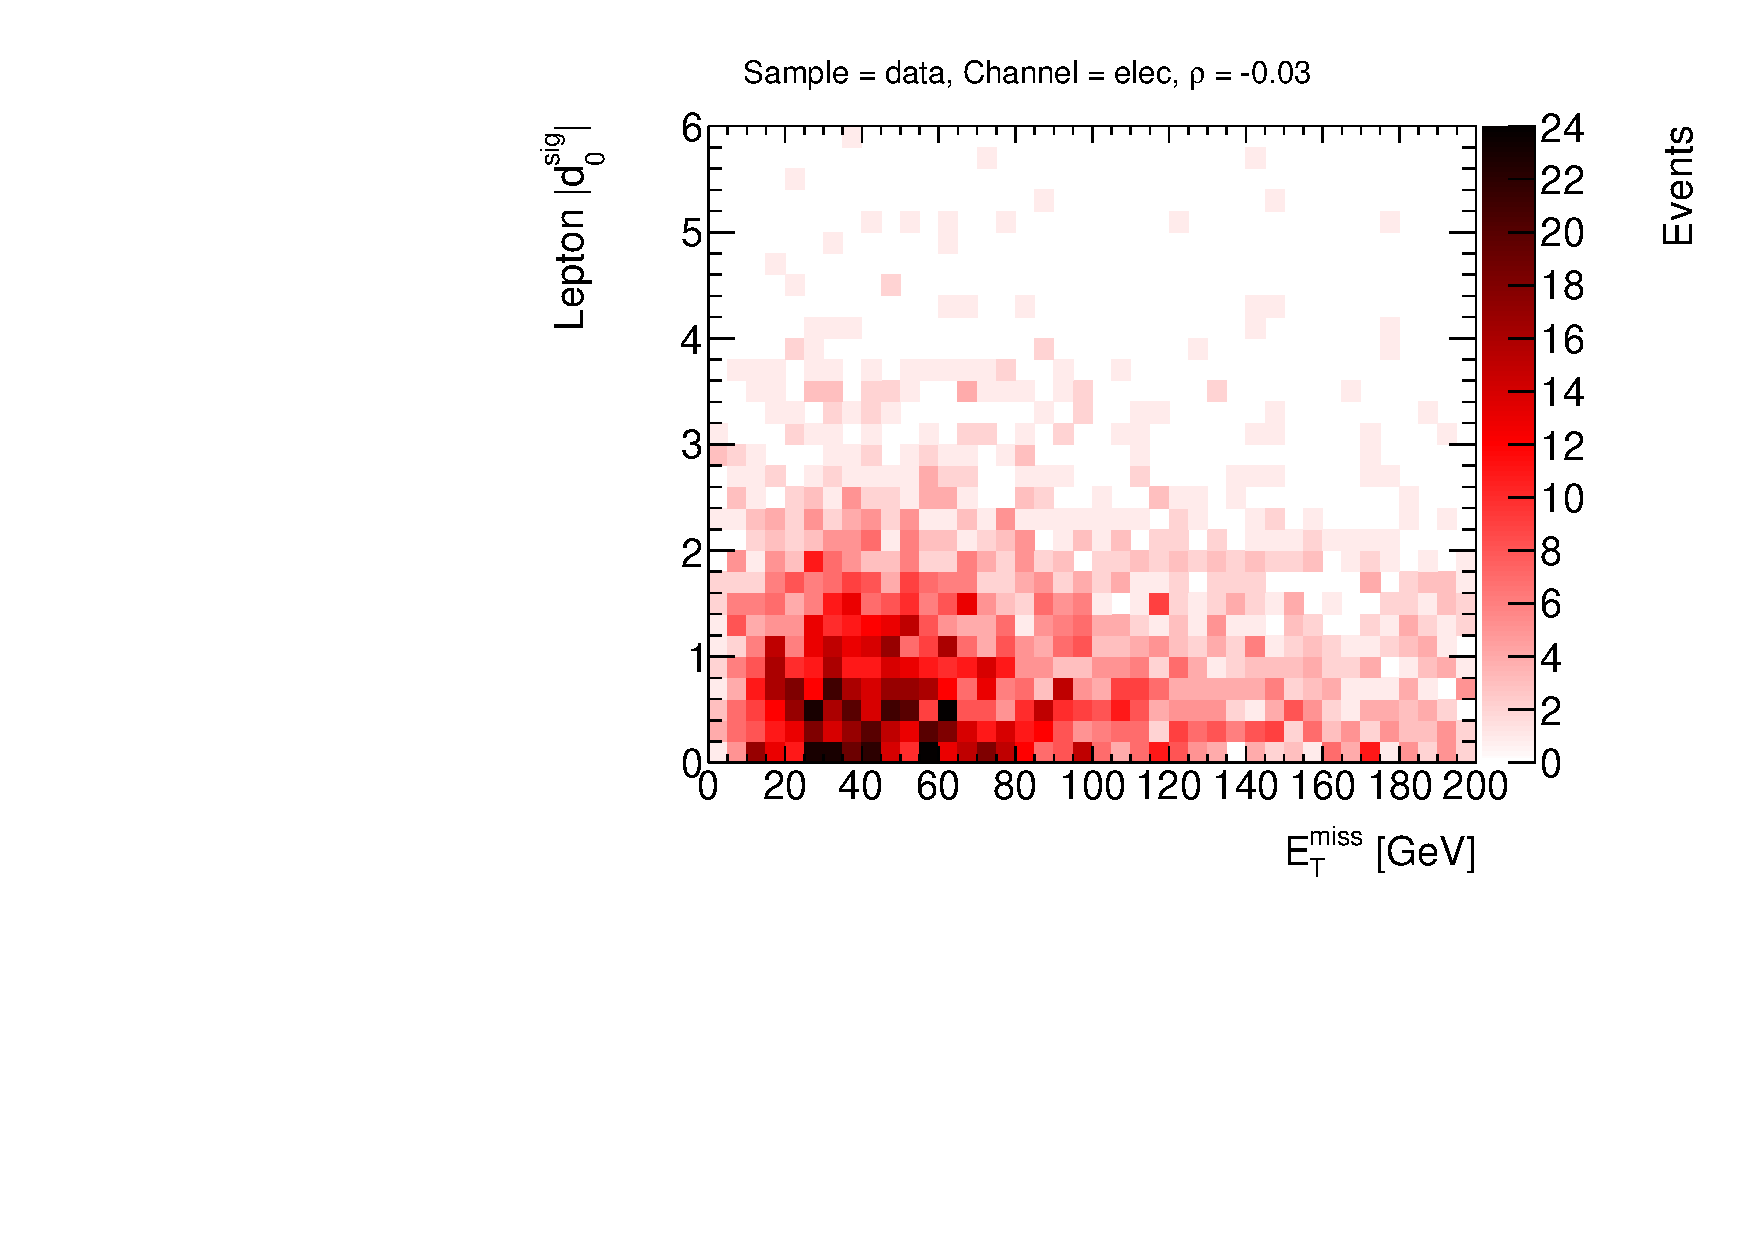
\includegraphics[scale=0.33]{./figures/boosted/ABCD/h2_d0_met_elec_data}
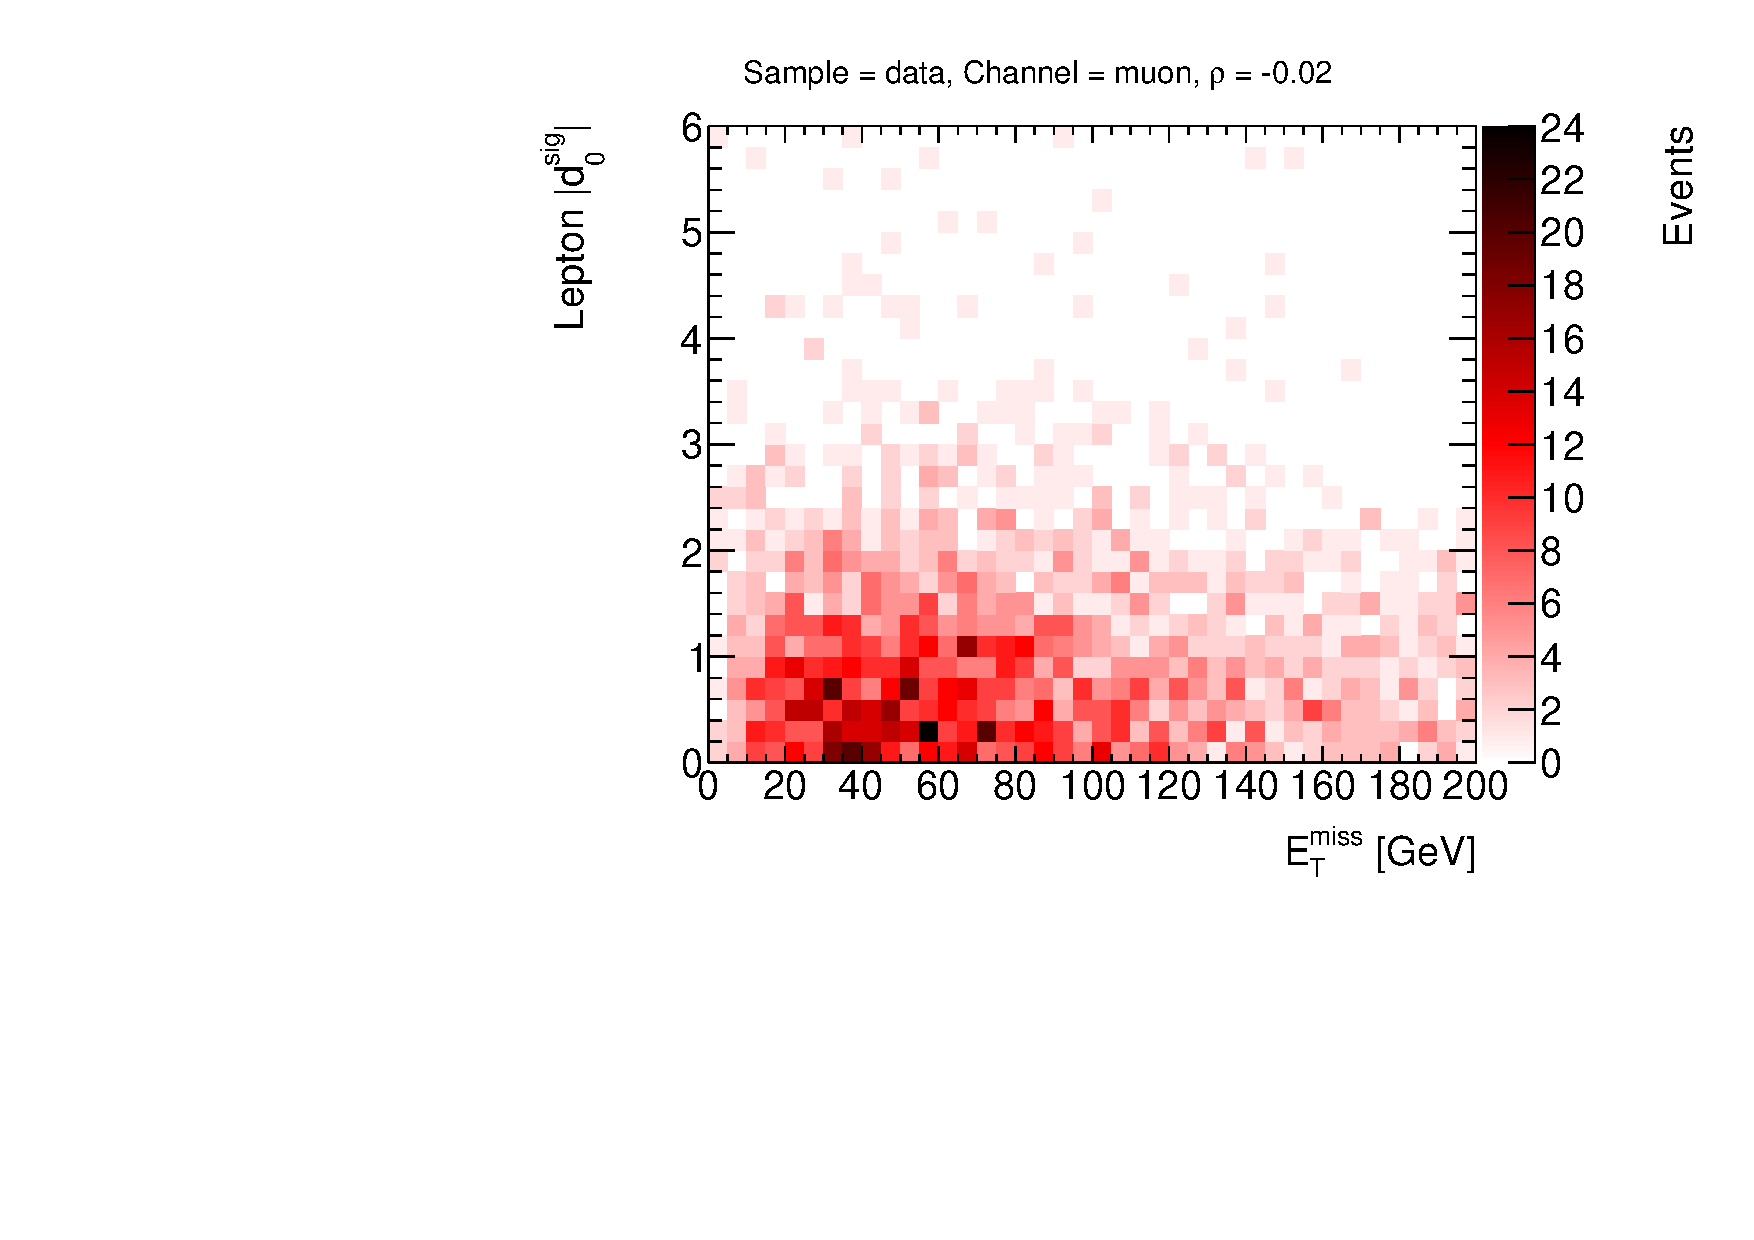
\includegraphics[scale=0.33]{./figures/boosted/ABCD/h2_d0_met_muon_data}
\caption{$|d_{0}^{\textrm{sig}}|$ vs \met distribution for data in each lepton channel. $\rho$ is the correlation factor
as computed using ROOT's TH2F::GetCorrelationFactor() method.}
\label{fig:boosted_qcd_d0met_data}
\end{center}
\end{figure}


\begin{figure}[!htbp]
\begin{center}
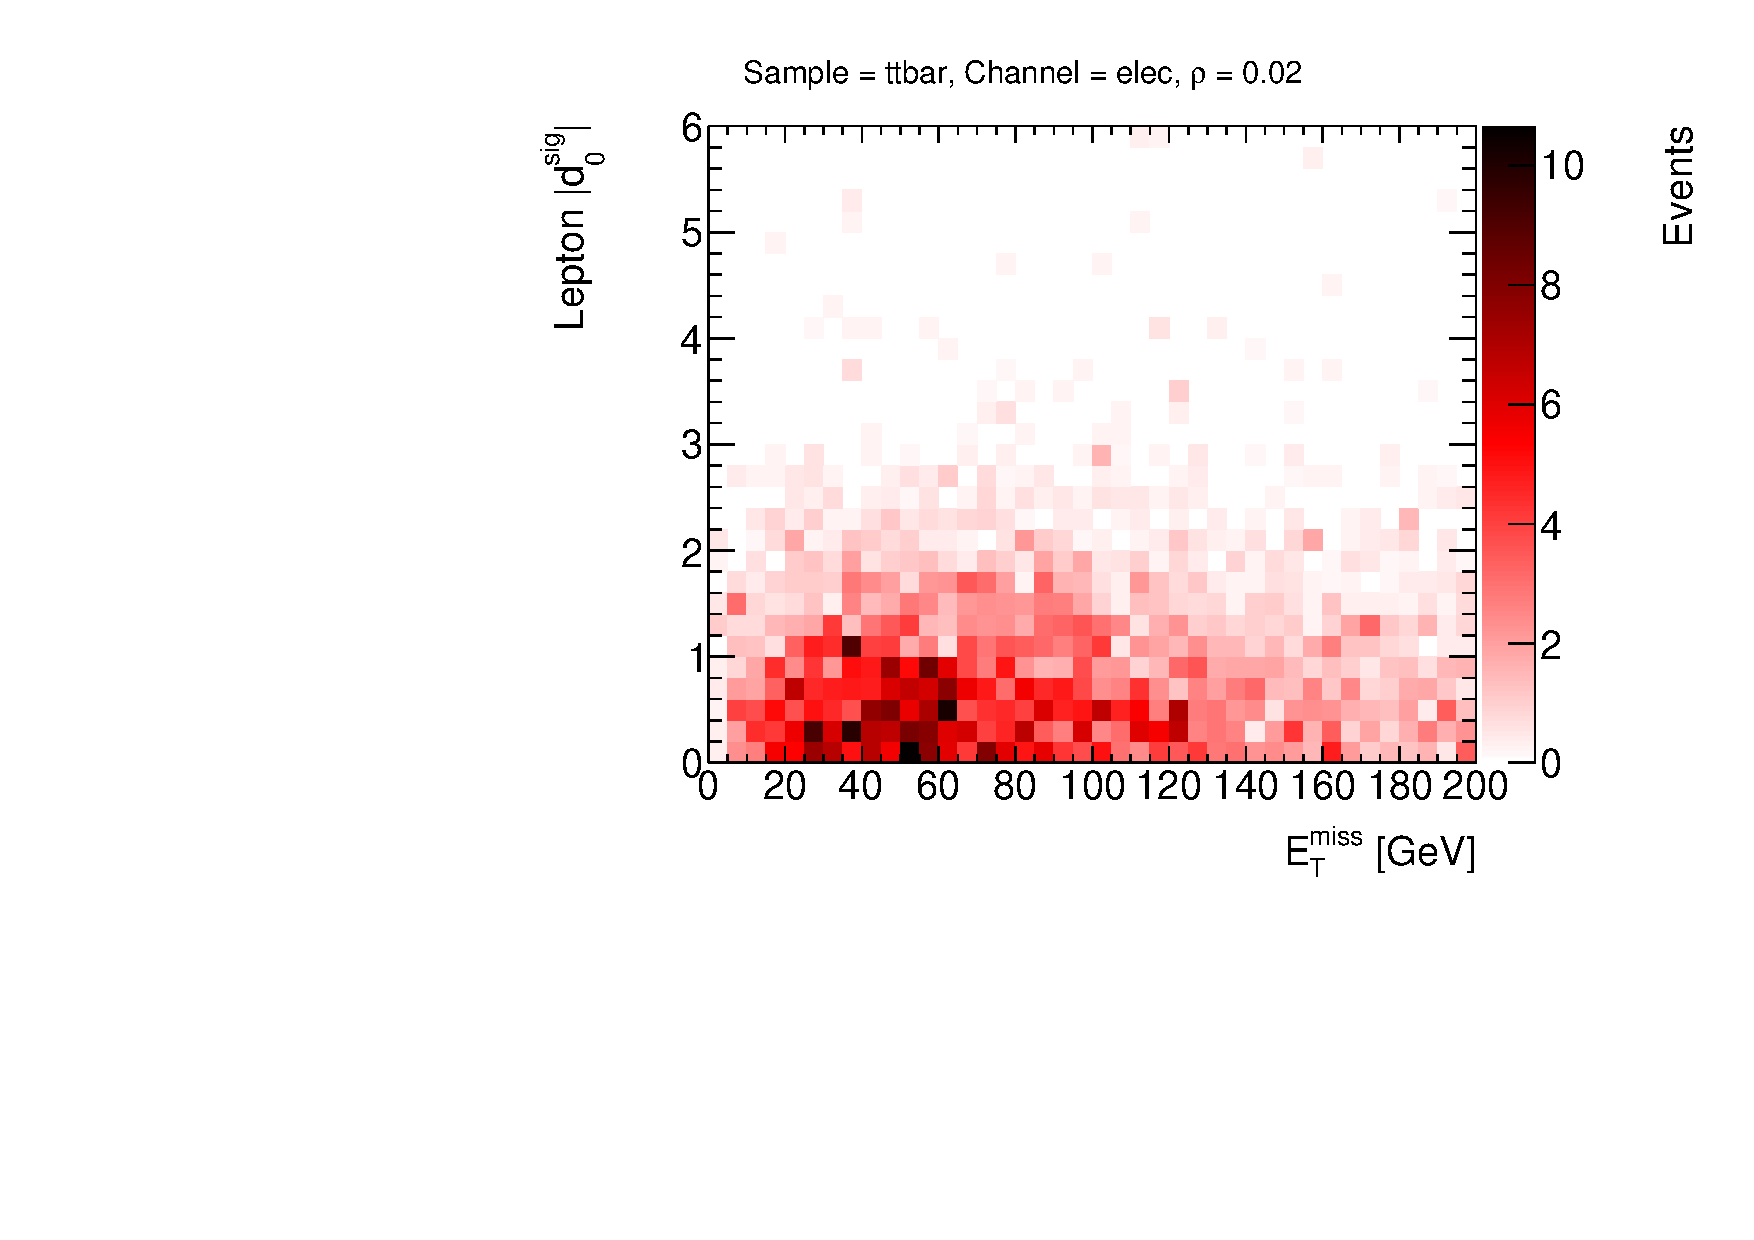
\includegraphics[scale=0.33]{./figures/boosted/ABCD/h2_d0_met_elec_ttbar}
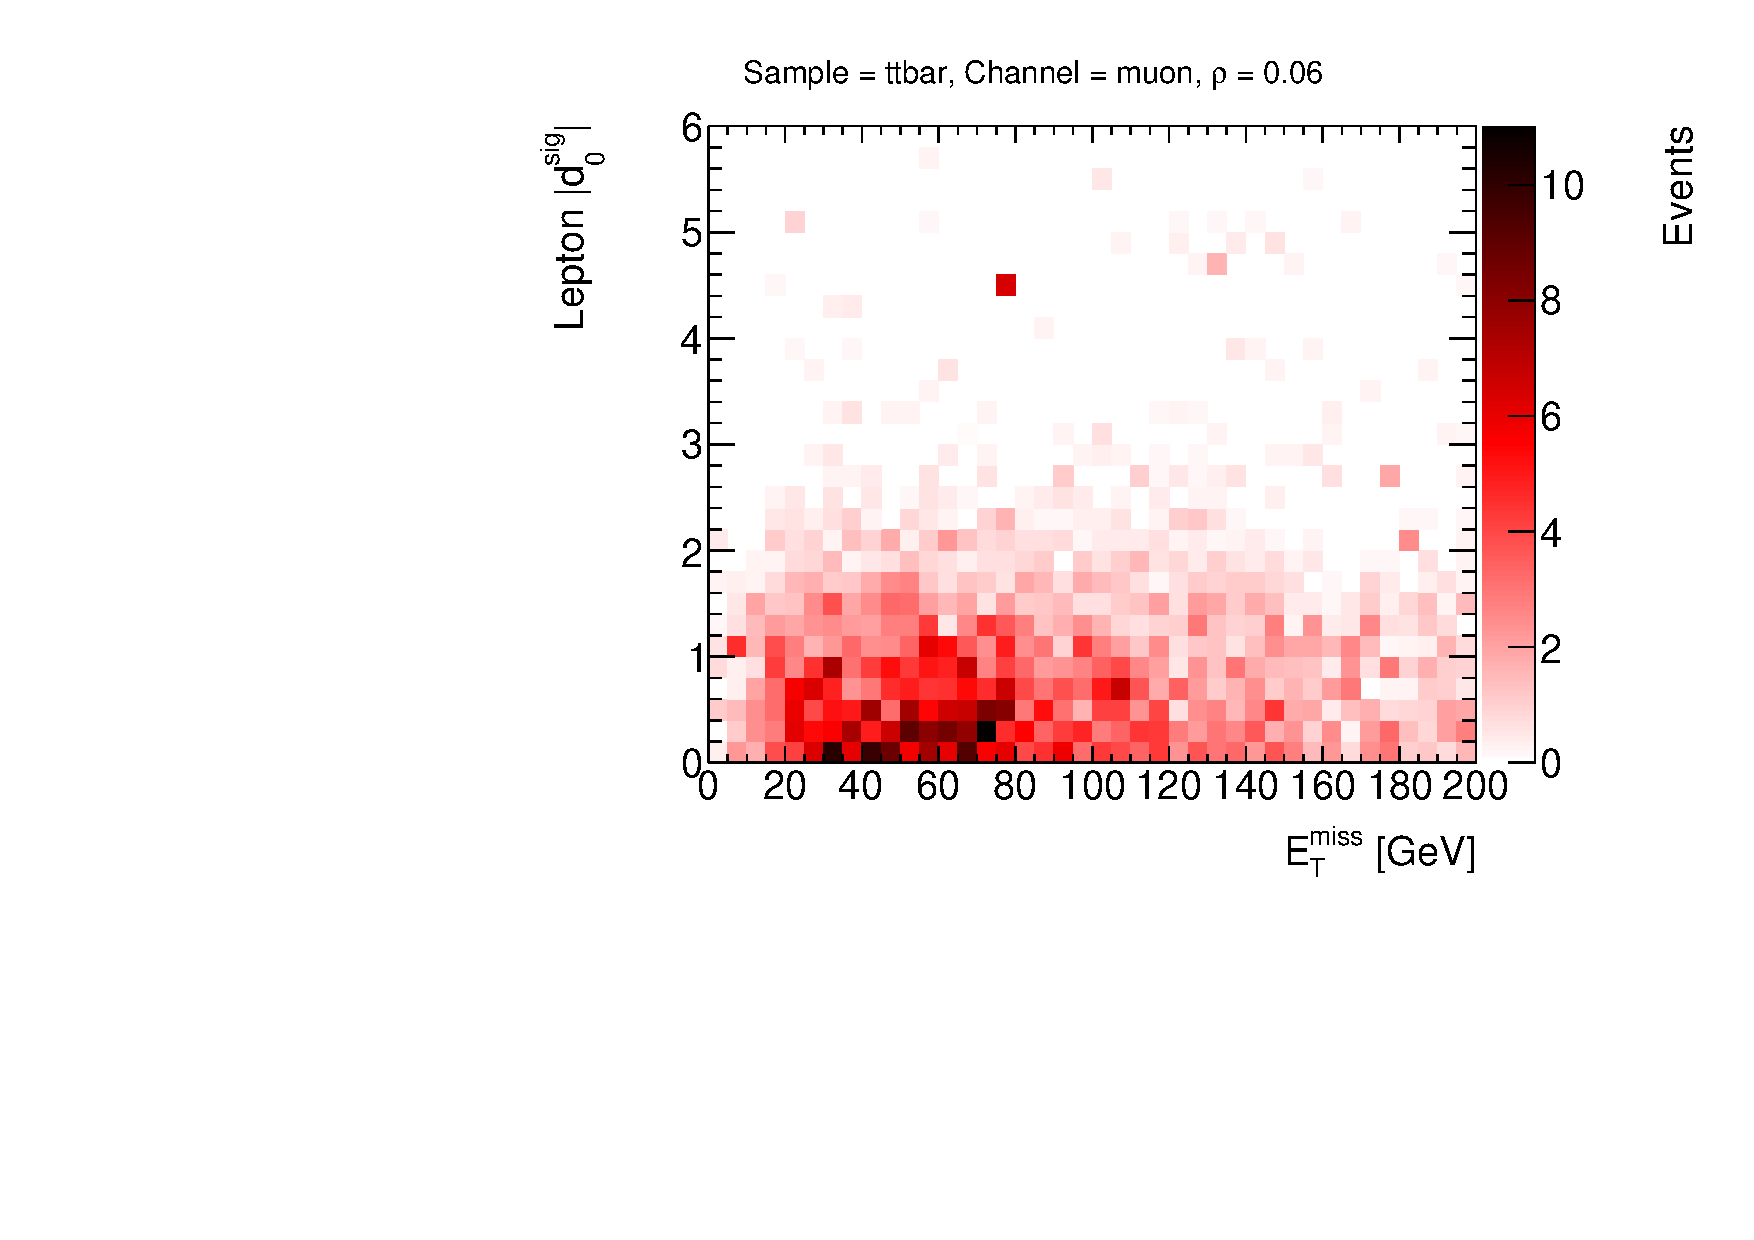
\includegraphics[scale=0.33]{./figures/boosted/ABCD/h2_d0_met_muon_ttbar}\\
\par\medskip
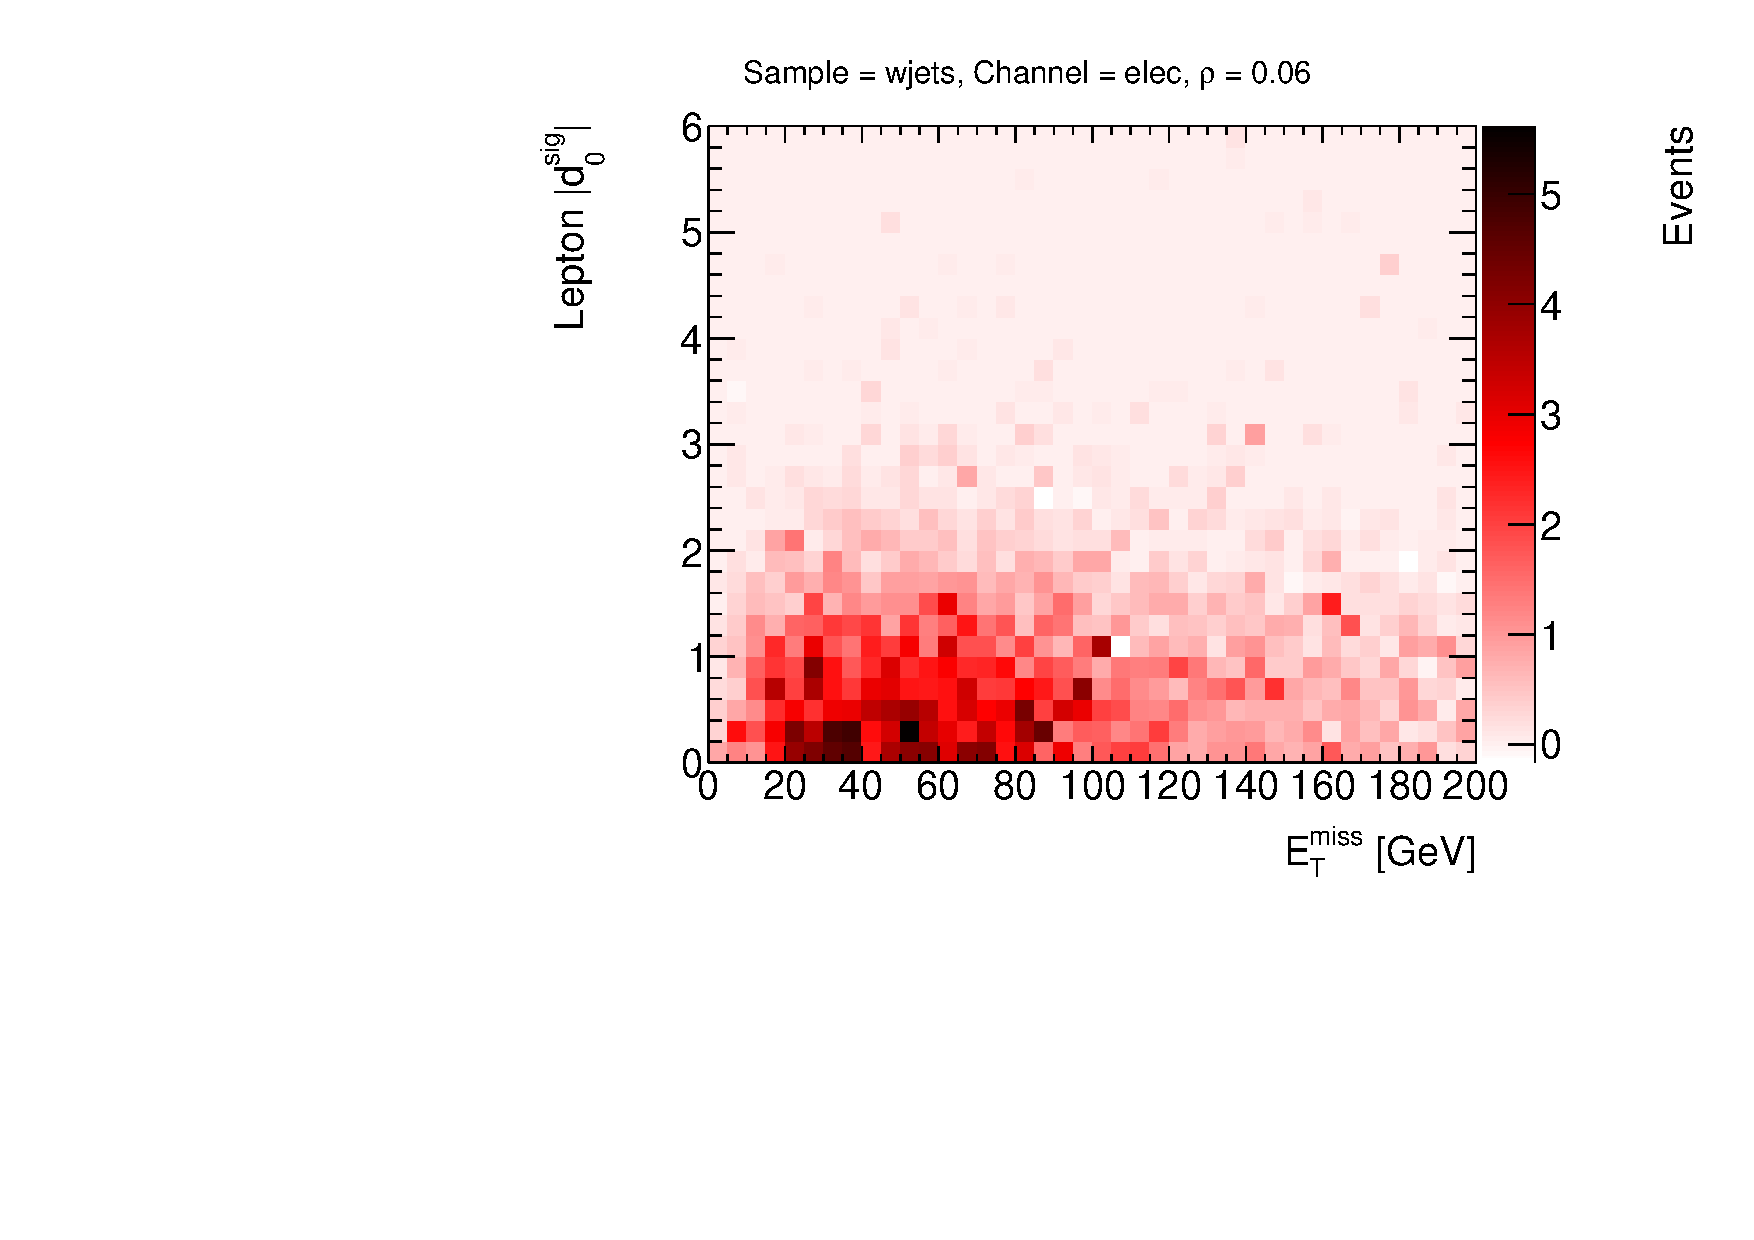
\includegraphics[scale=0.33]{./figures/boosted/ABCD/h2_d0_met_elec_wjets}
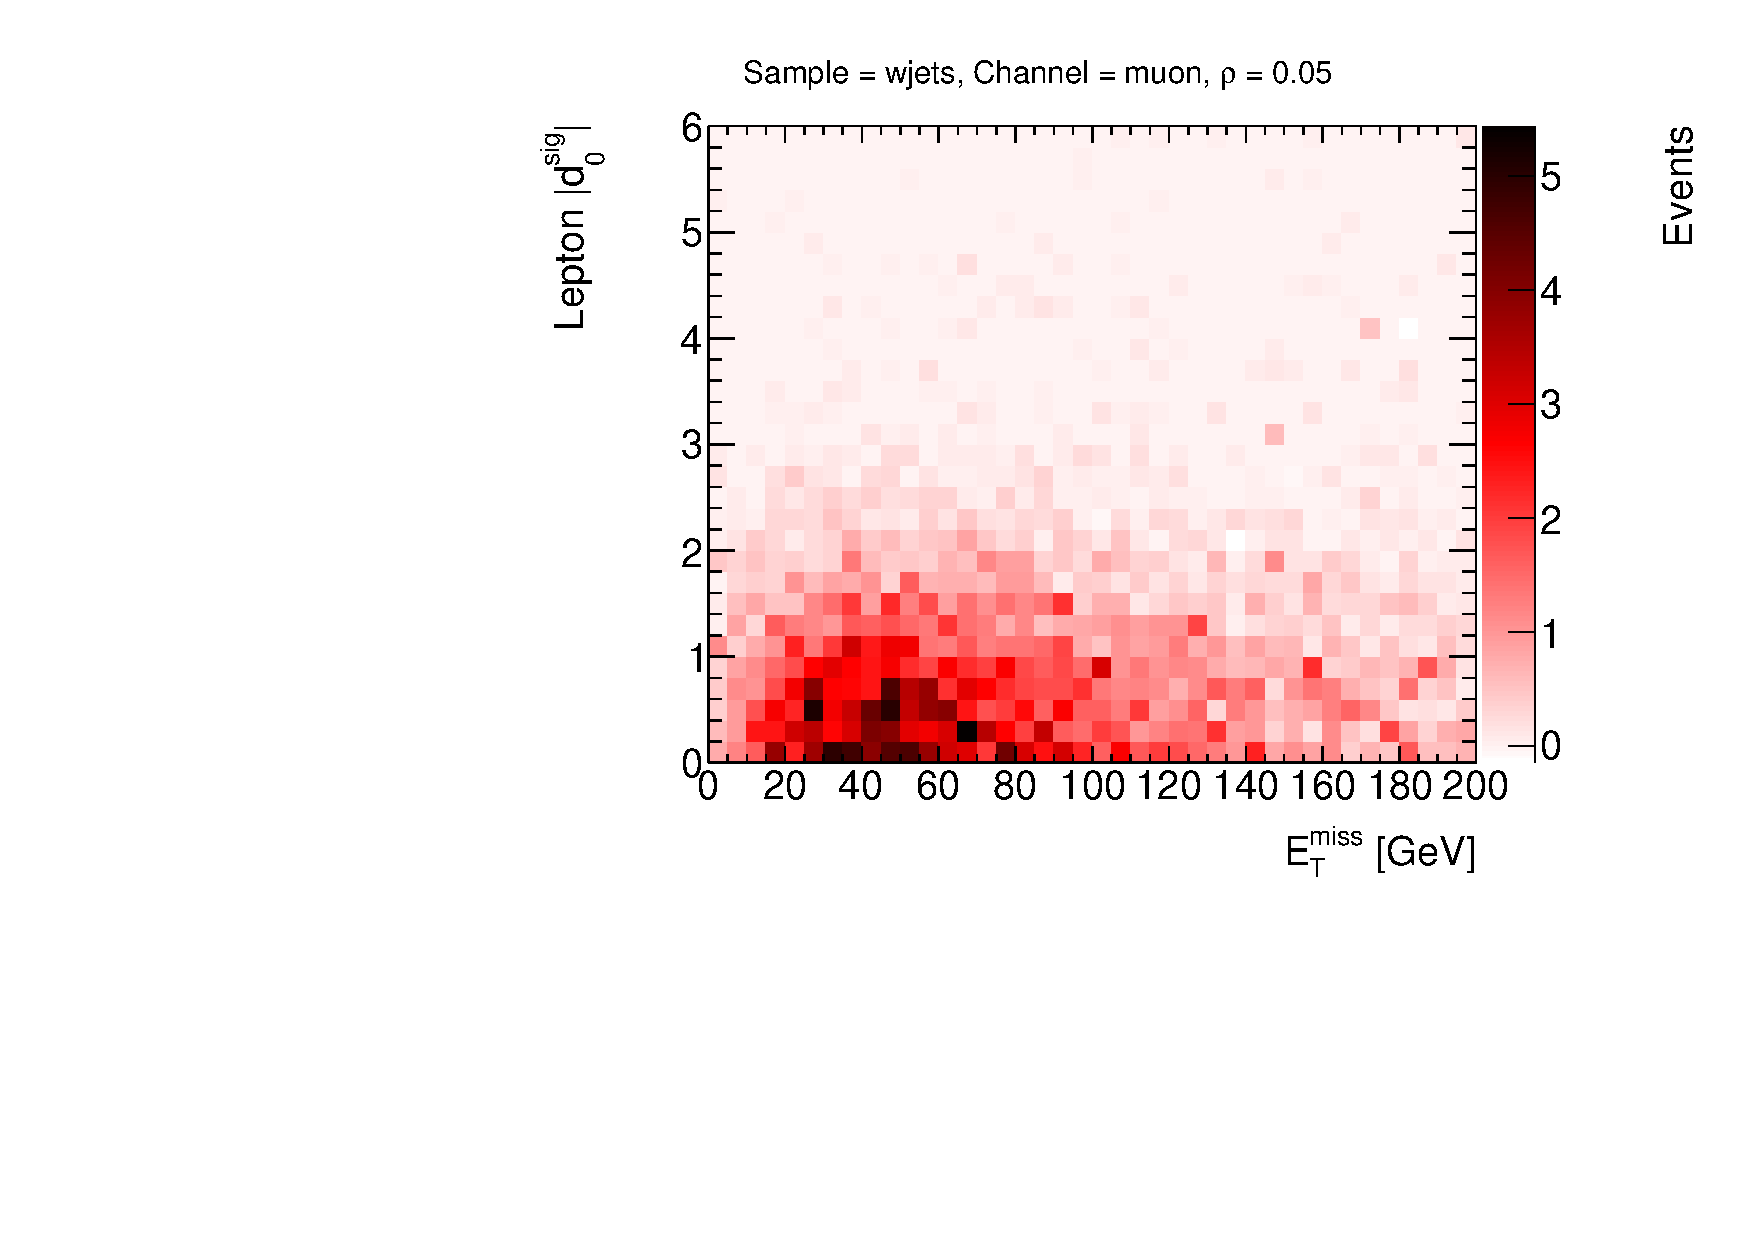
\includegraphics[scale=0.33]{./figures/boosted/ABCD/h2_d0_met_muon_wjets}\\
\par\medskip
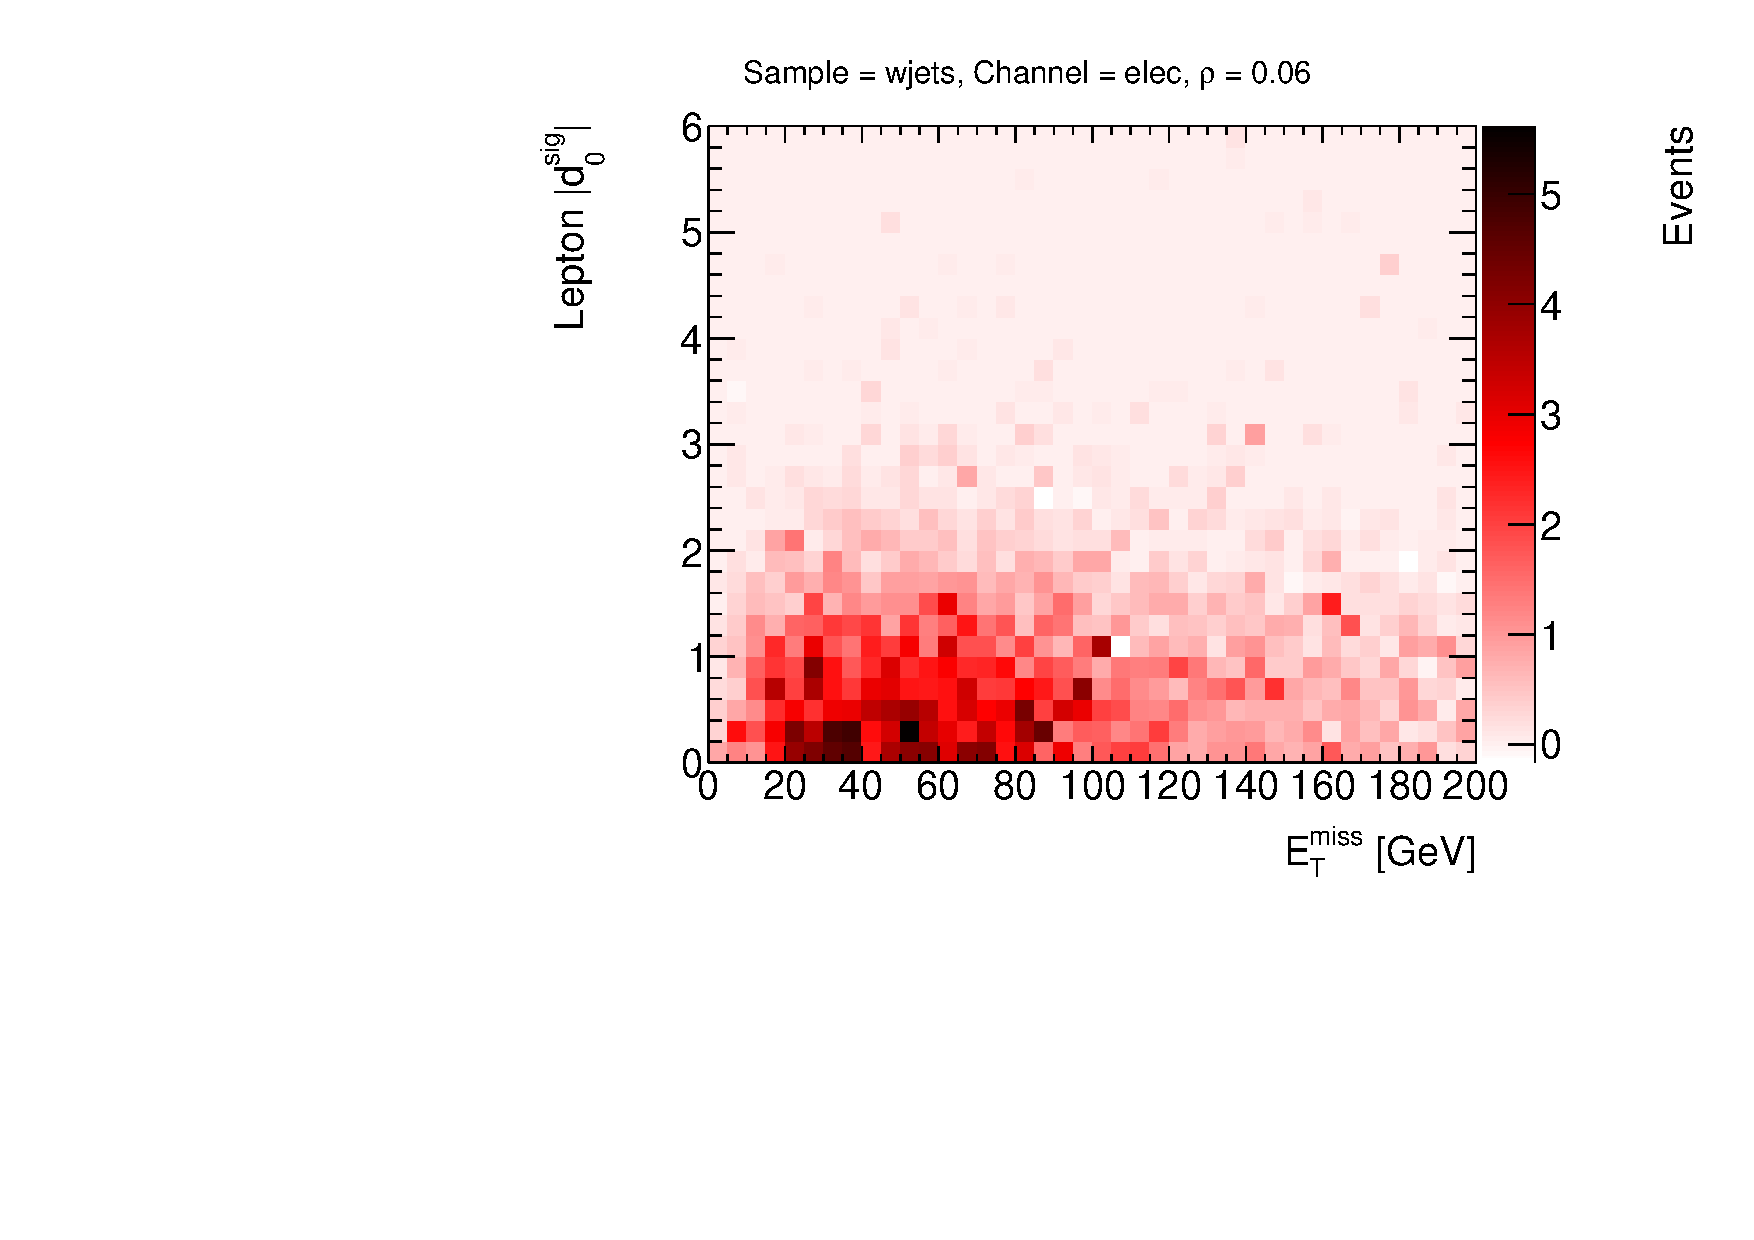
\includegraphics[scale=0.33]{./figures/boosted/ABCD/h2_d0_met_elec_wjets}
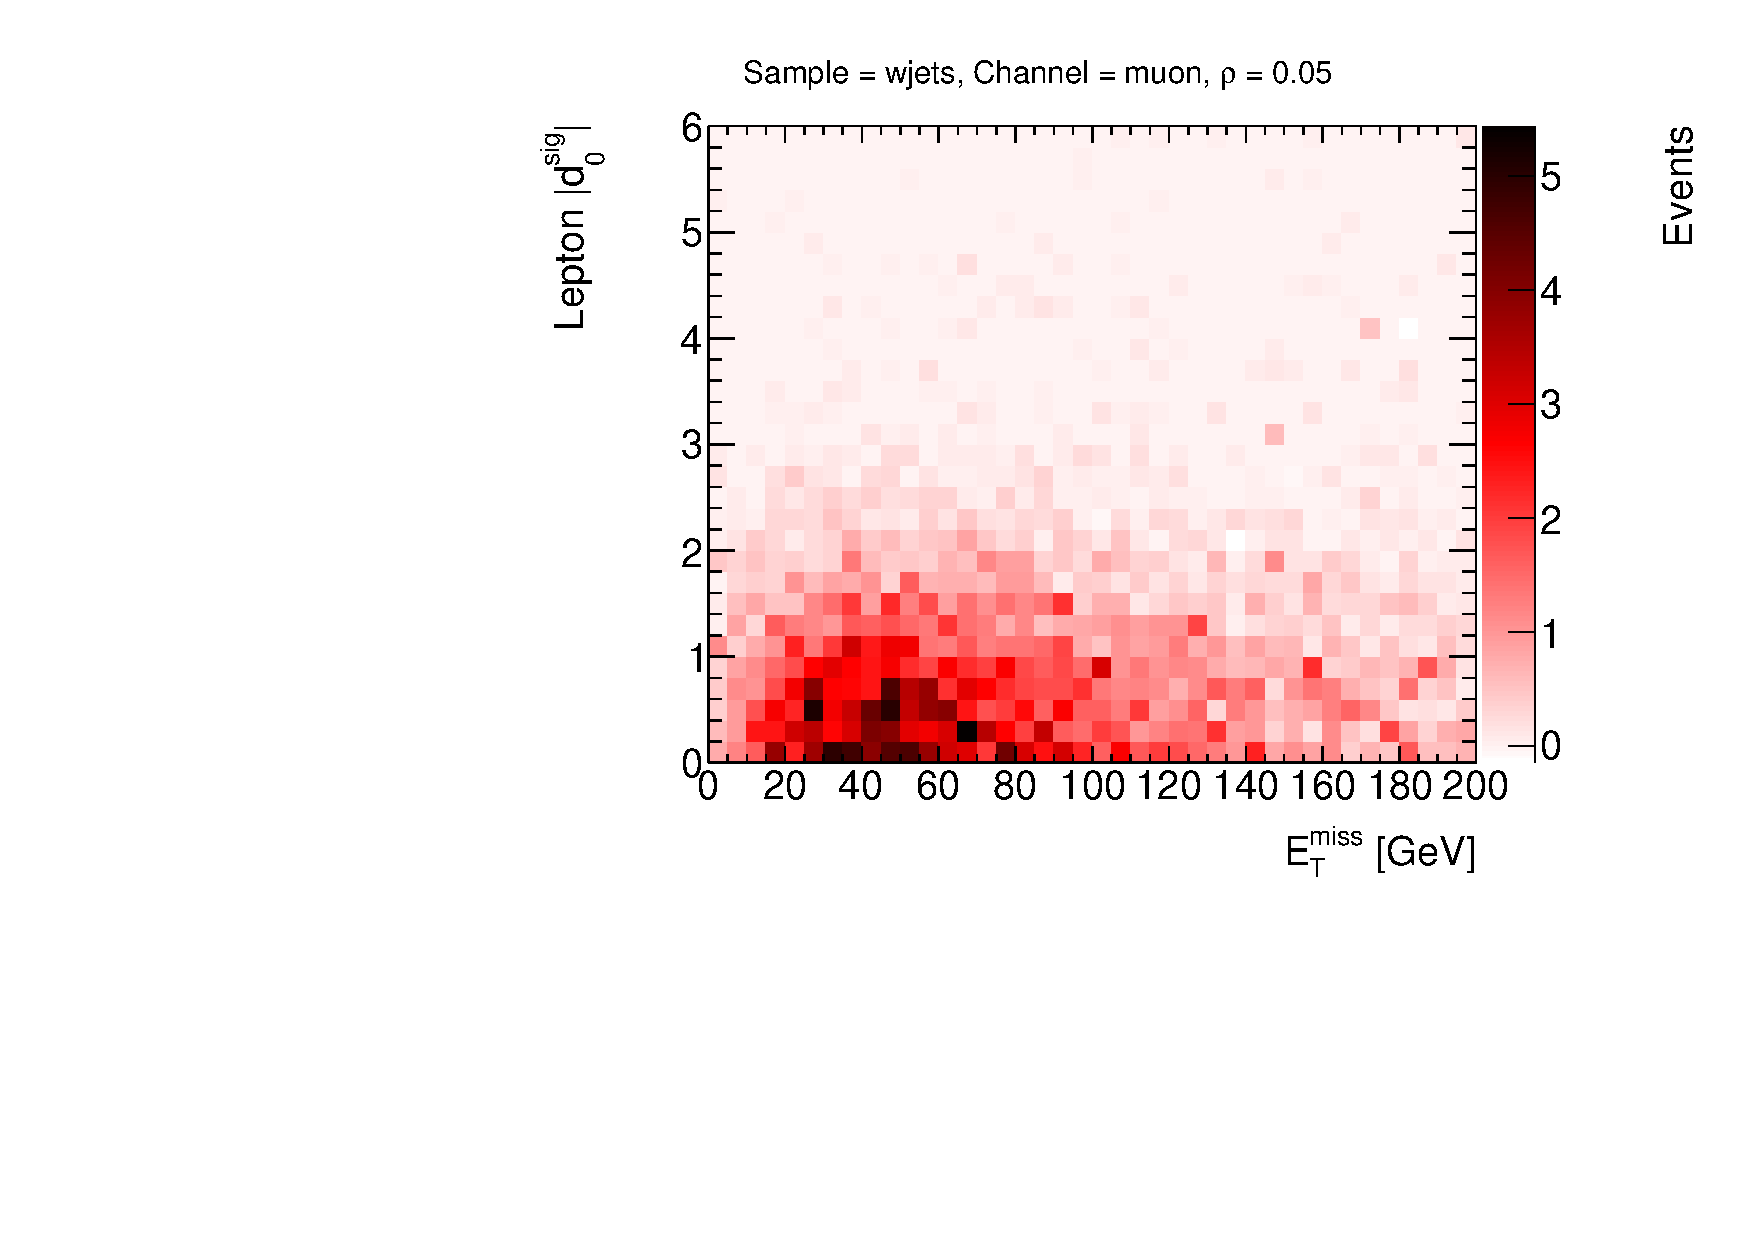
\includegraphics[scale=0.33]{./figures/boosted/ABCD/h2_d0_met_muon_wjets}\\
\caption{$|d_{0}^{\textrm{sig}}|$ vs \met distribution for different MC samples in each lepton channel. $\rho$ is the correlation factor
as computed using ROOT's TH2F::GetCorrelationFactor() method.}
\label{fig:boosted_qcd_d0met_mc}
\end{center}
\end{figure}


\FloatBarrier
%%%%%%%%%%%%%%%%%%%%%%%%%%%%%%
%
% 2-tag vs 1-tag comparisons
%
%%%%%%%%%%%%%%%%%%%%%%%%%%%%%%
\subsection{Shape template: 2-tag vs 1-tag comparison}
\label{app:boosted_qcd_2tag1tag}

Figure~\ref{fig:boosted_abcd_2tag1tag} shows comparisons between 2-tag and 1-tag multijet templates (i.e background subtracted data) 
in region C of the ABCD method for several kinematic distributions in the signal region and mBB control region. As can be seen in 
all the distributions, the statistical uncertainties of the 2-tag multijet template are large and and suffers from bin-by-bin fluctuations
which make the 2-tag templates unsuitable to provide reasonable shape prediction in region A. On the other hand, the 1-tag templates statistical
uncertainties are smaller and provide smoother distributions. 

\begin{figure}[!htbp]
\begin{center}
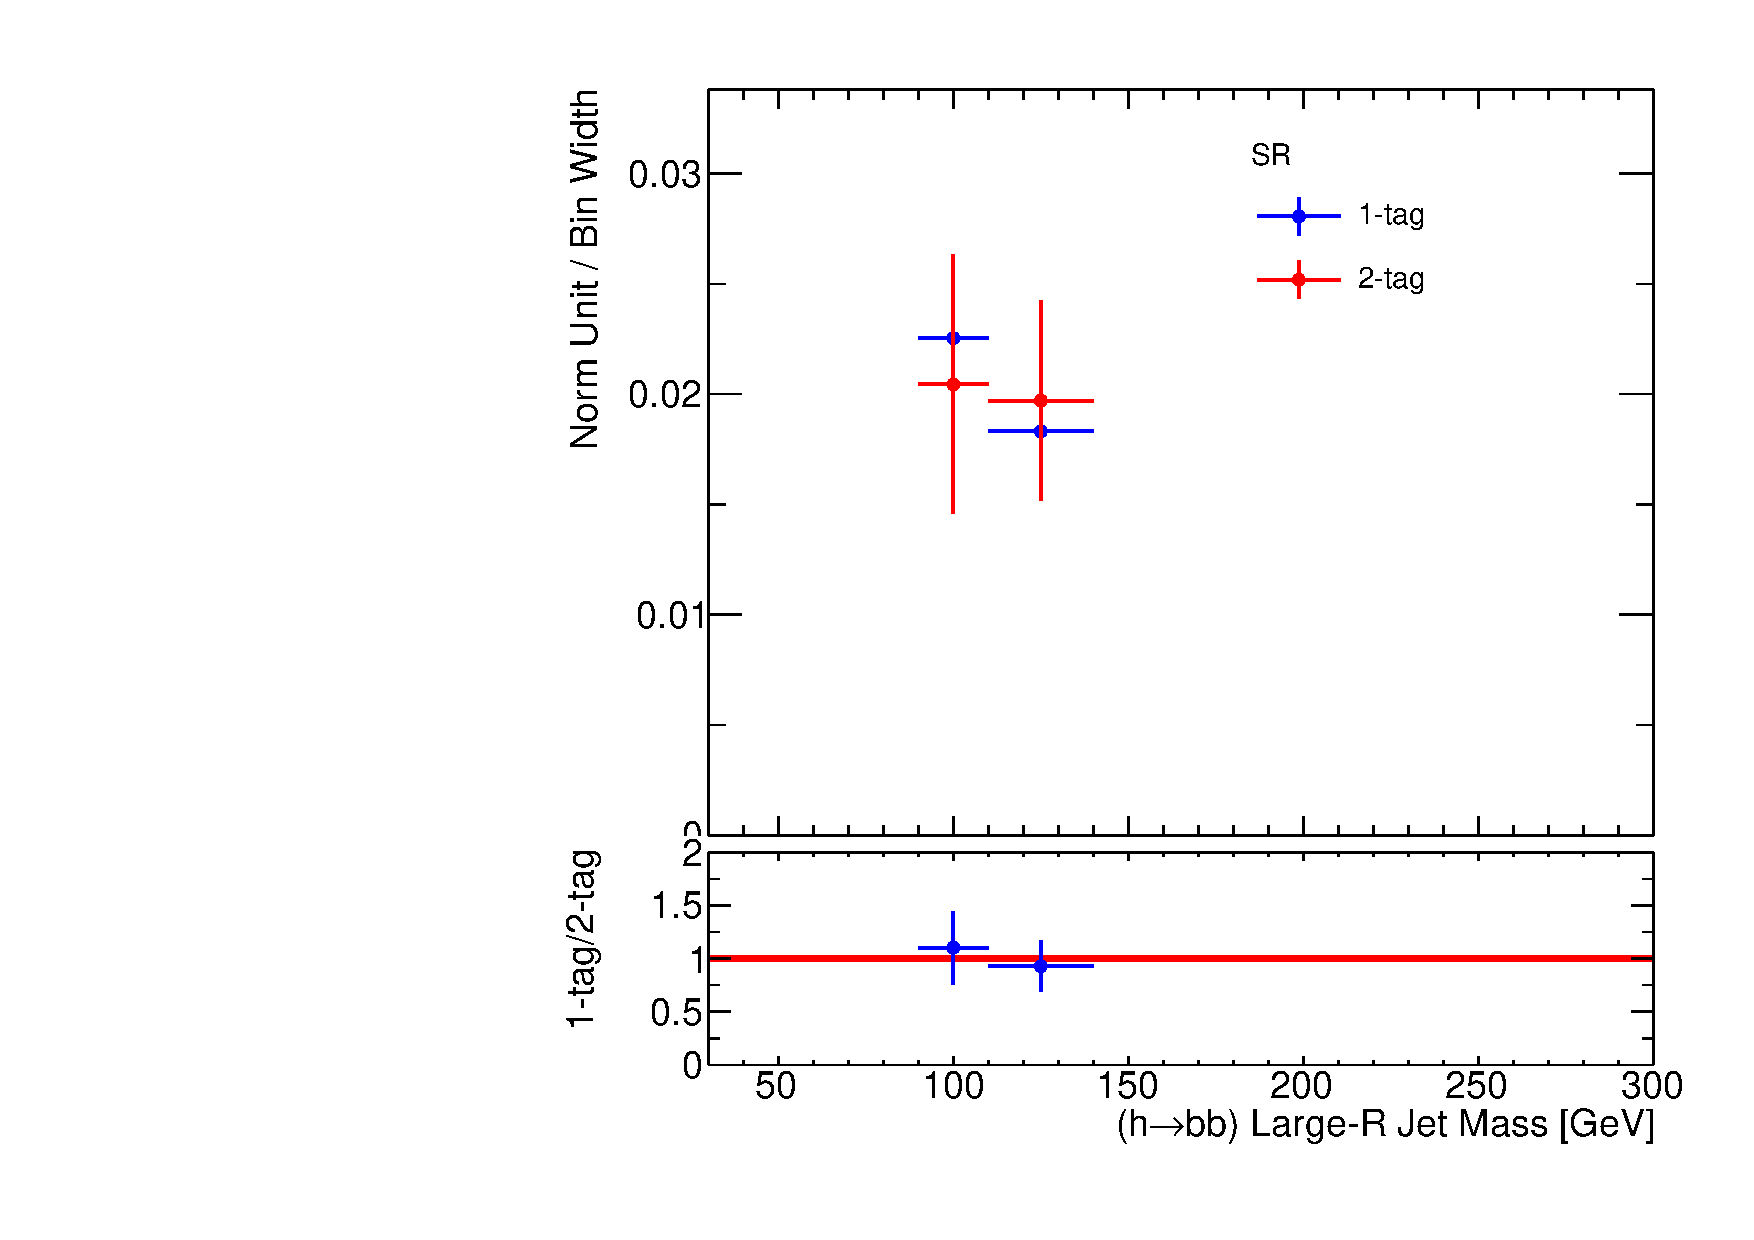
\includegraphics[scale=0.33]{./figures/boosted/ABCD/ABCD_2TagVs1Tag_SR_lepton_HbbMass}    
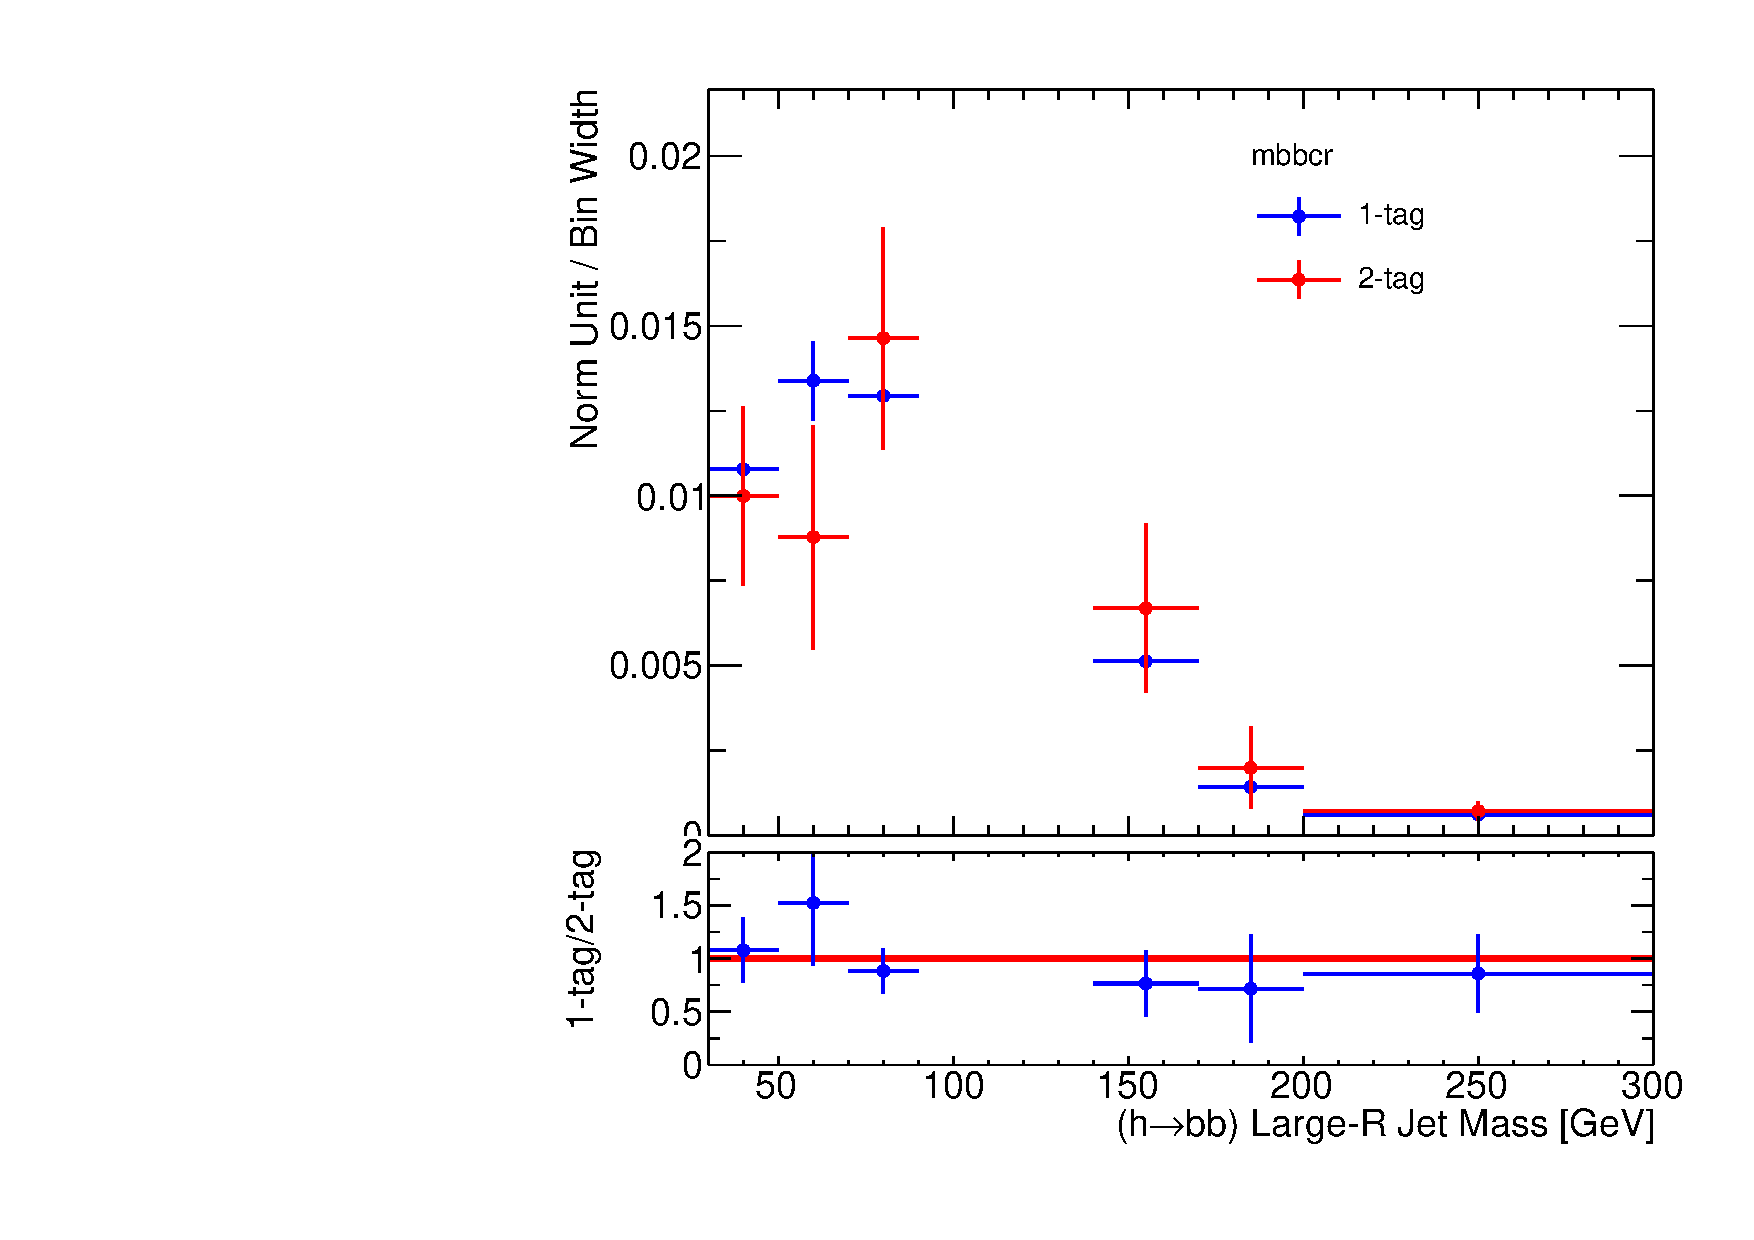
\includegraphics[scale=0.33]{./figures/boosted/ABCD/ABCD_2TagVs1Tag_mbbcr_lepton_HbbMass}\\
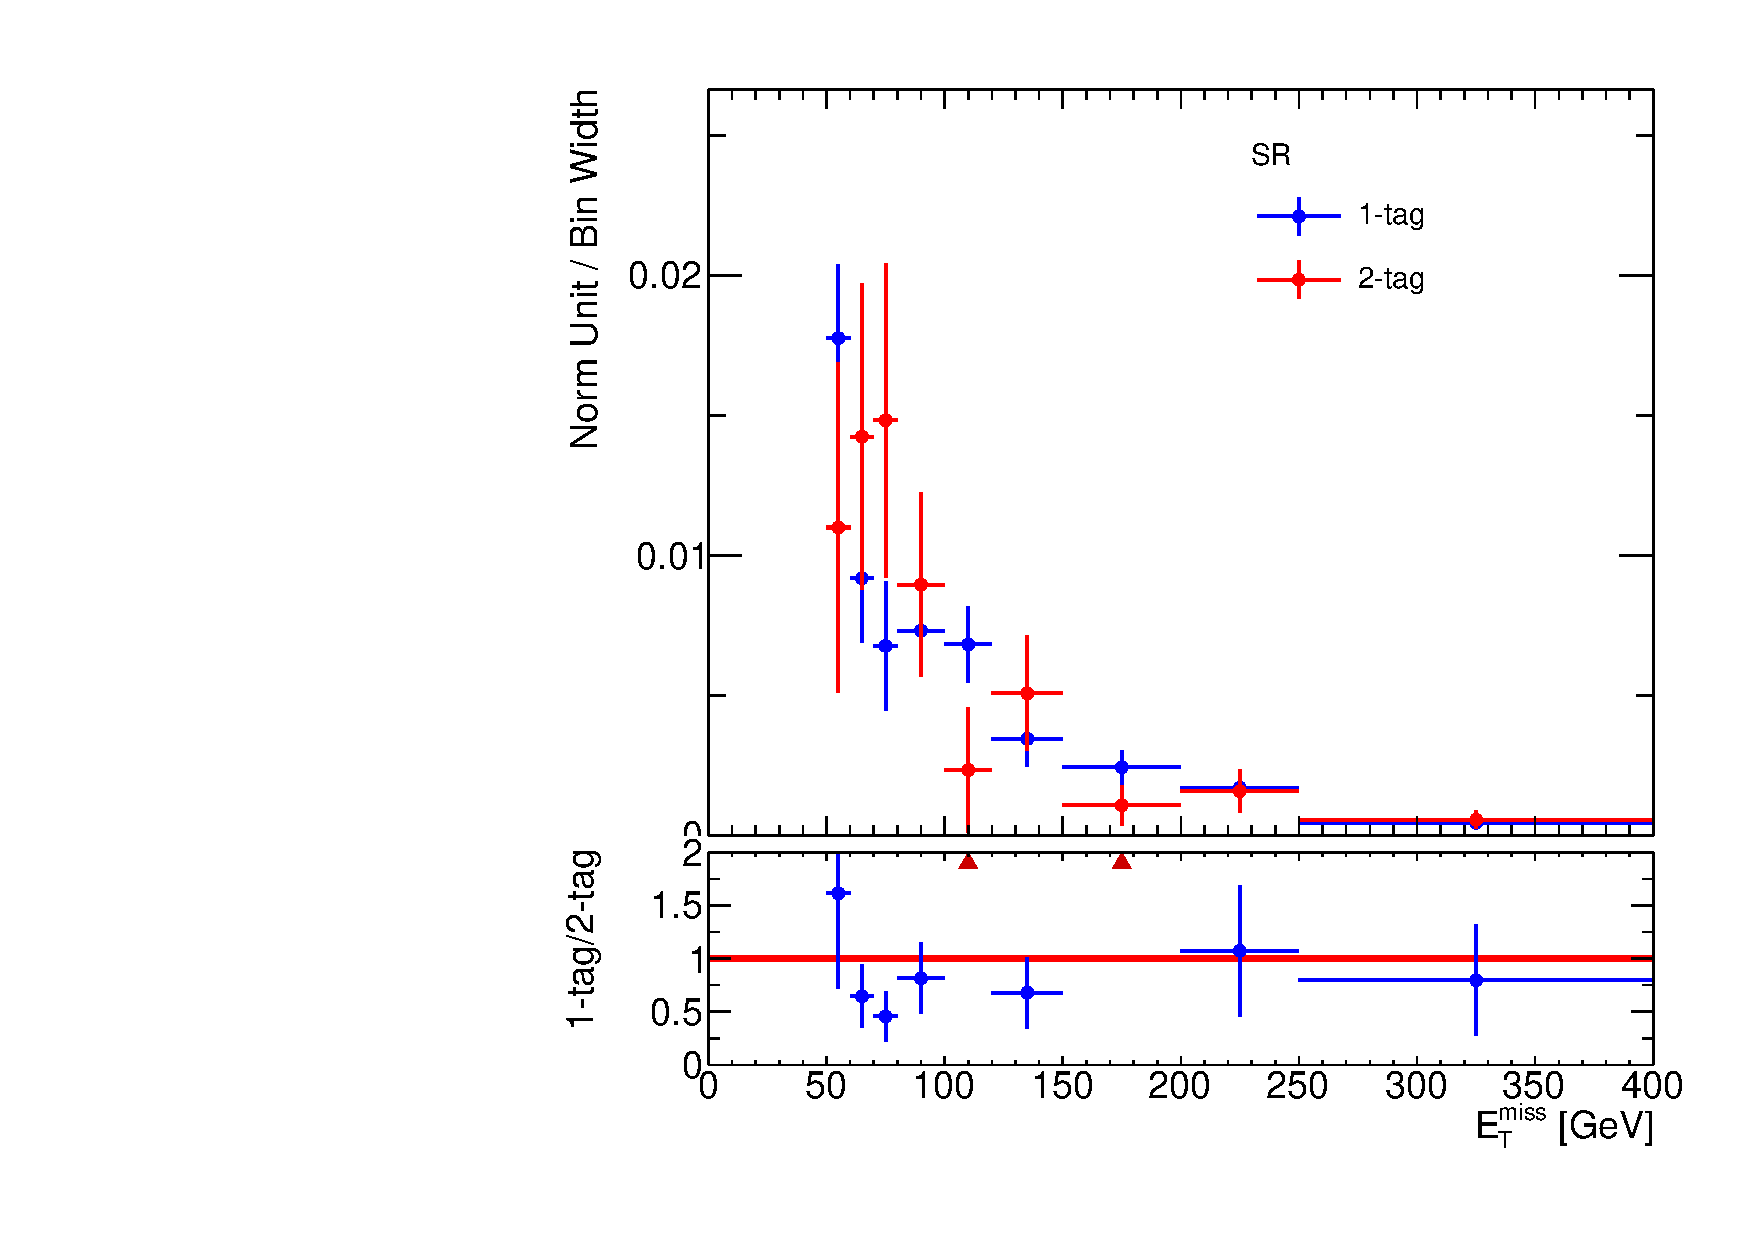
\includegraphics[scale=0.33]{./figures/boosted/ABCD/ABCD_2TagVs1Tag_SR_lepton_MET}   
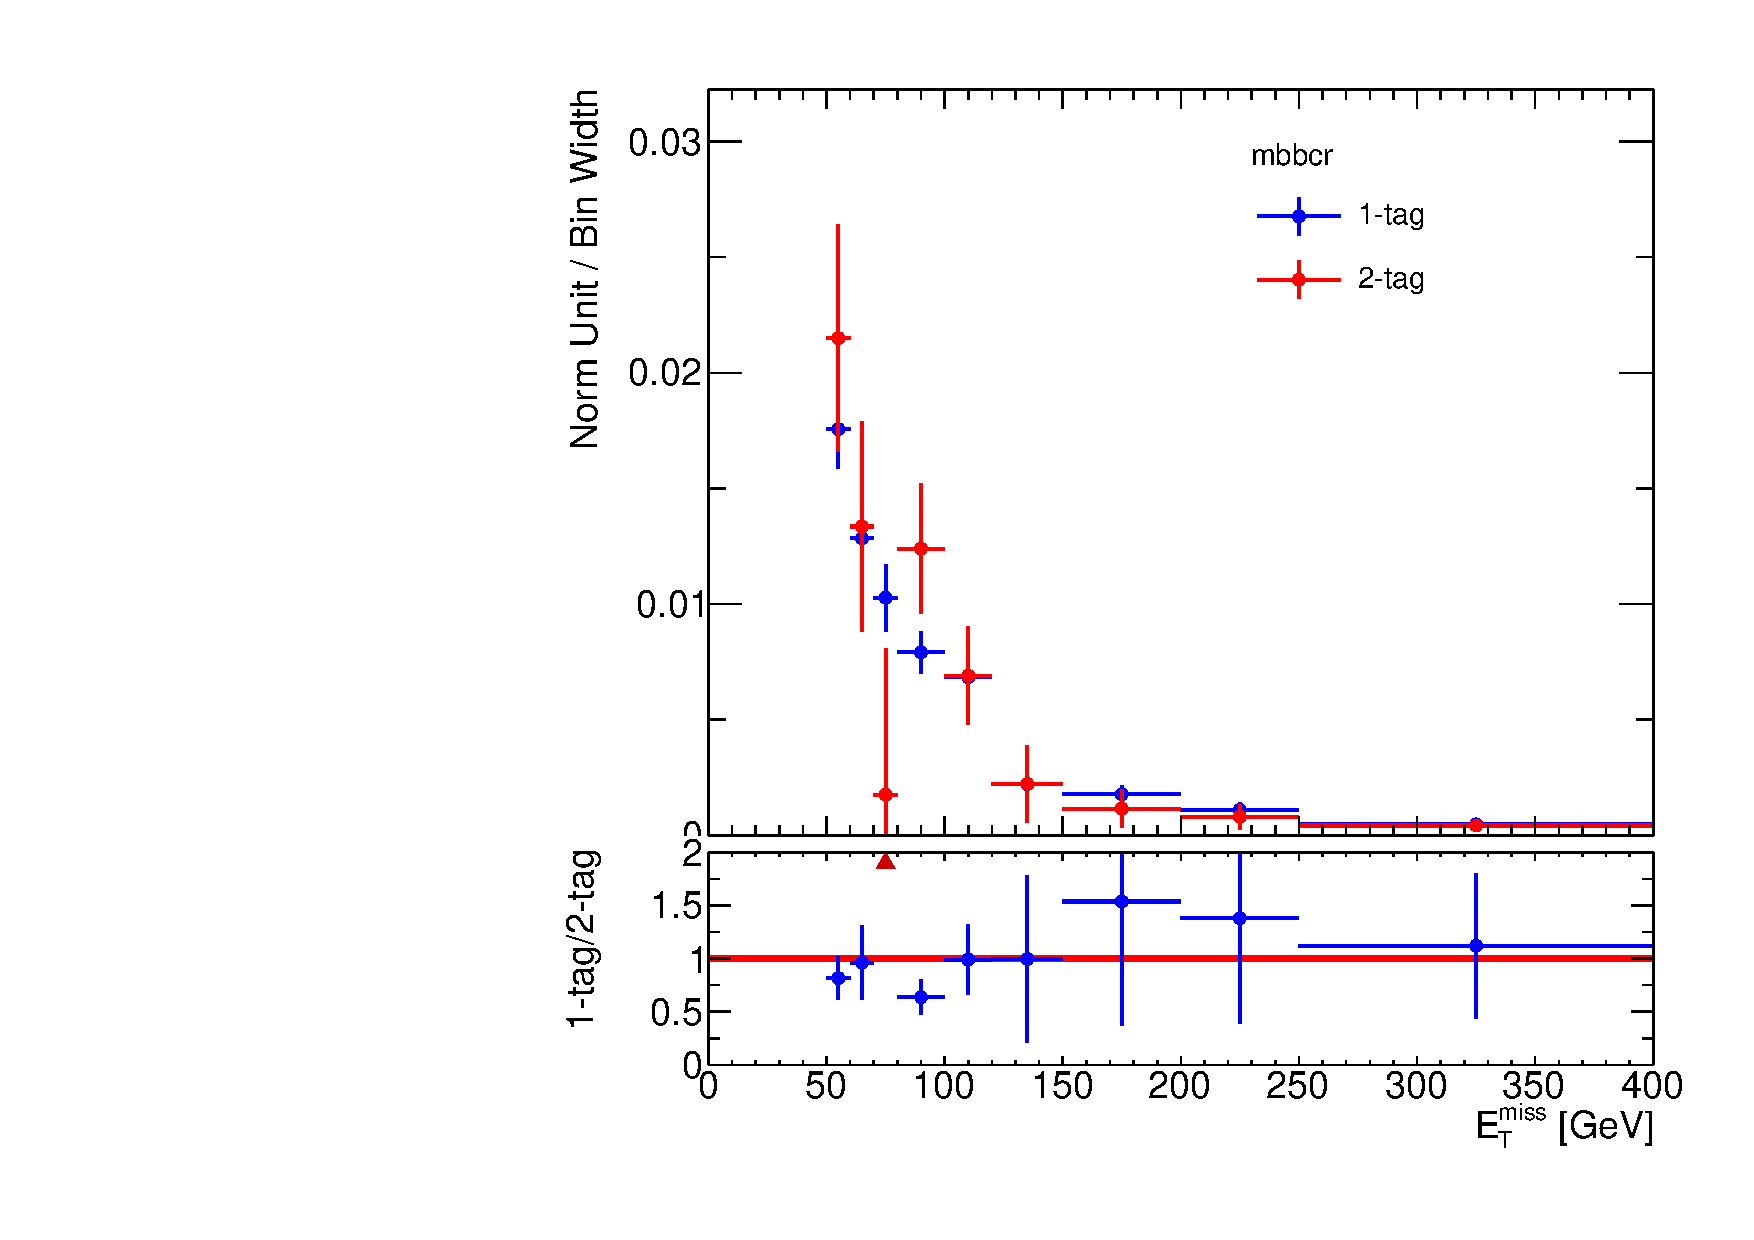
\includegraphics[scale=0.33]{./figures/boosted/ABCD/ABCD_2TagVs1Tag_mbbcr_lepton_MET}\\
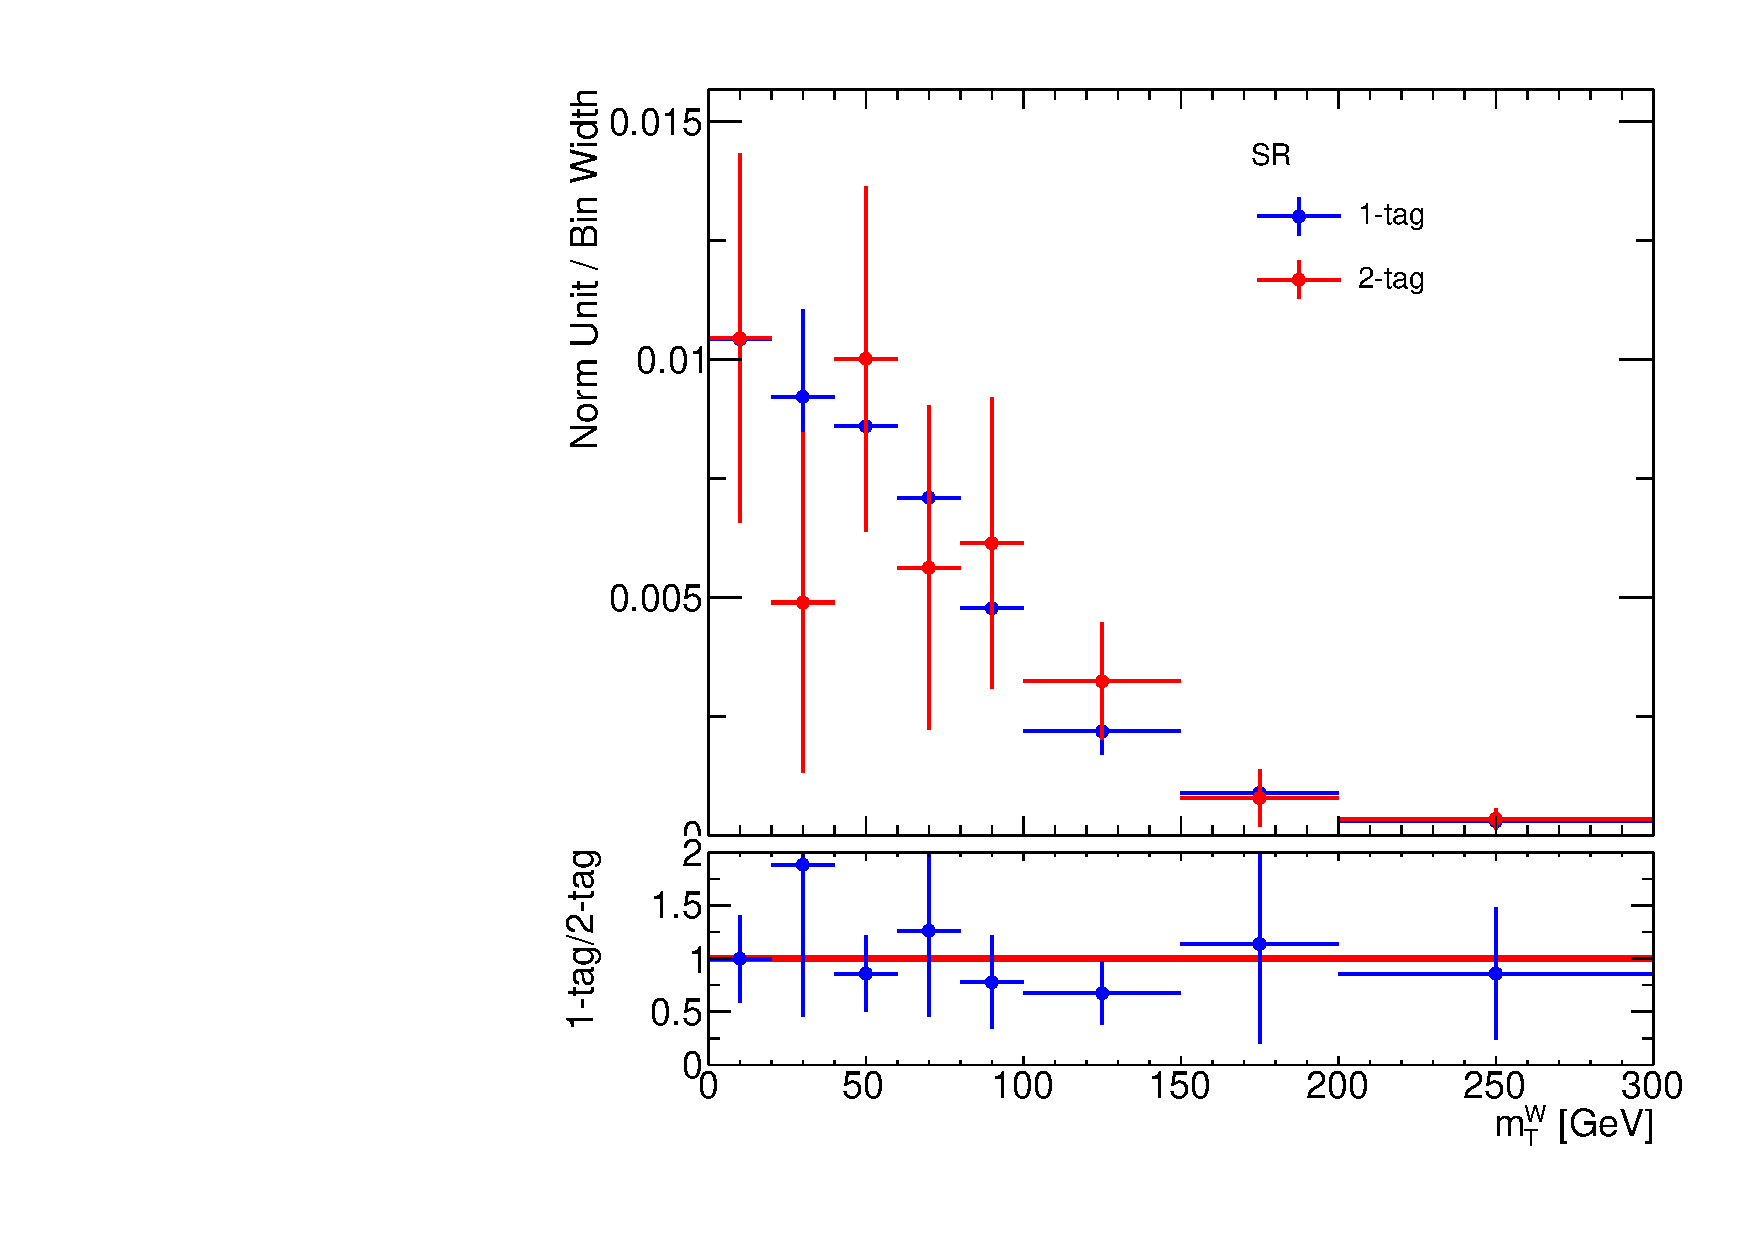
\includegraphics[scale=0.33]{./figures/boosted/ABCD/ABCD_2TagVs1Tag_SR_lepton_WlepMtATLAS} 
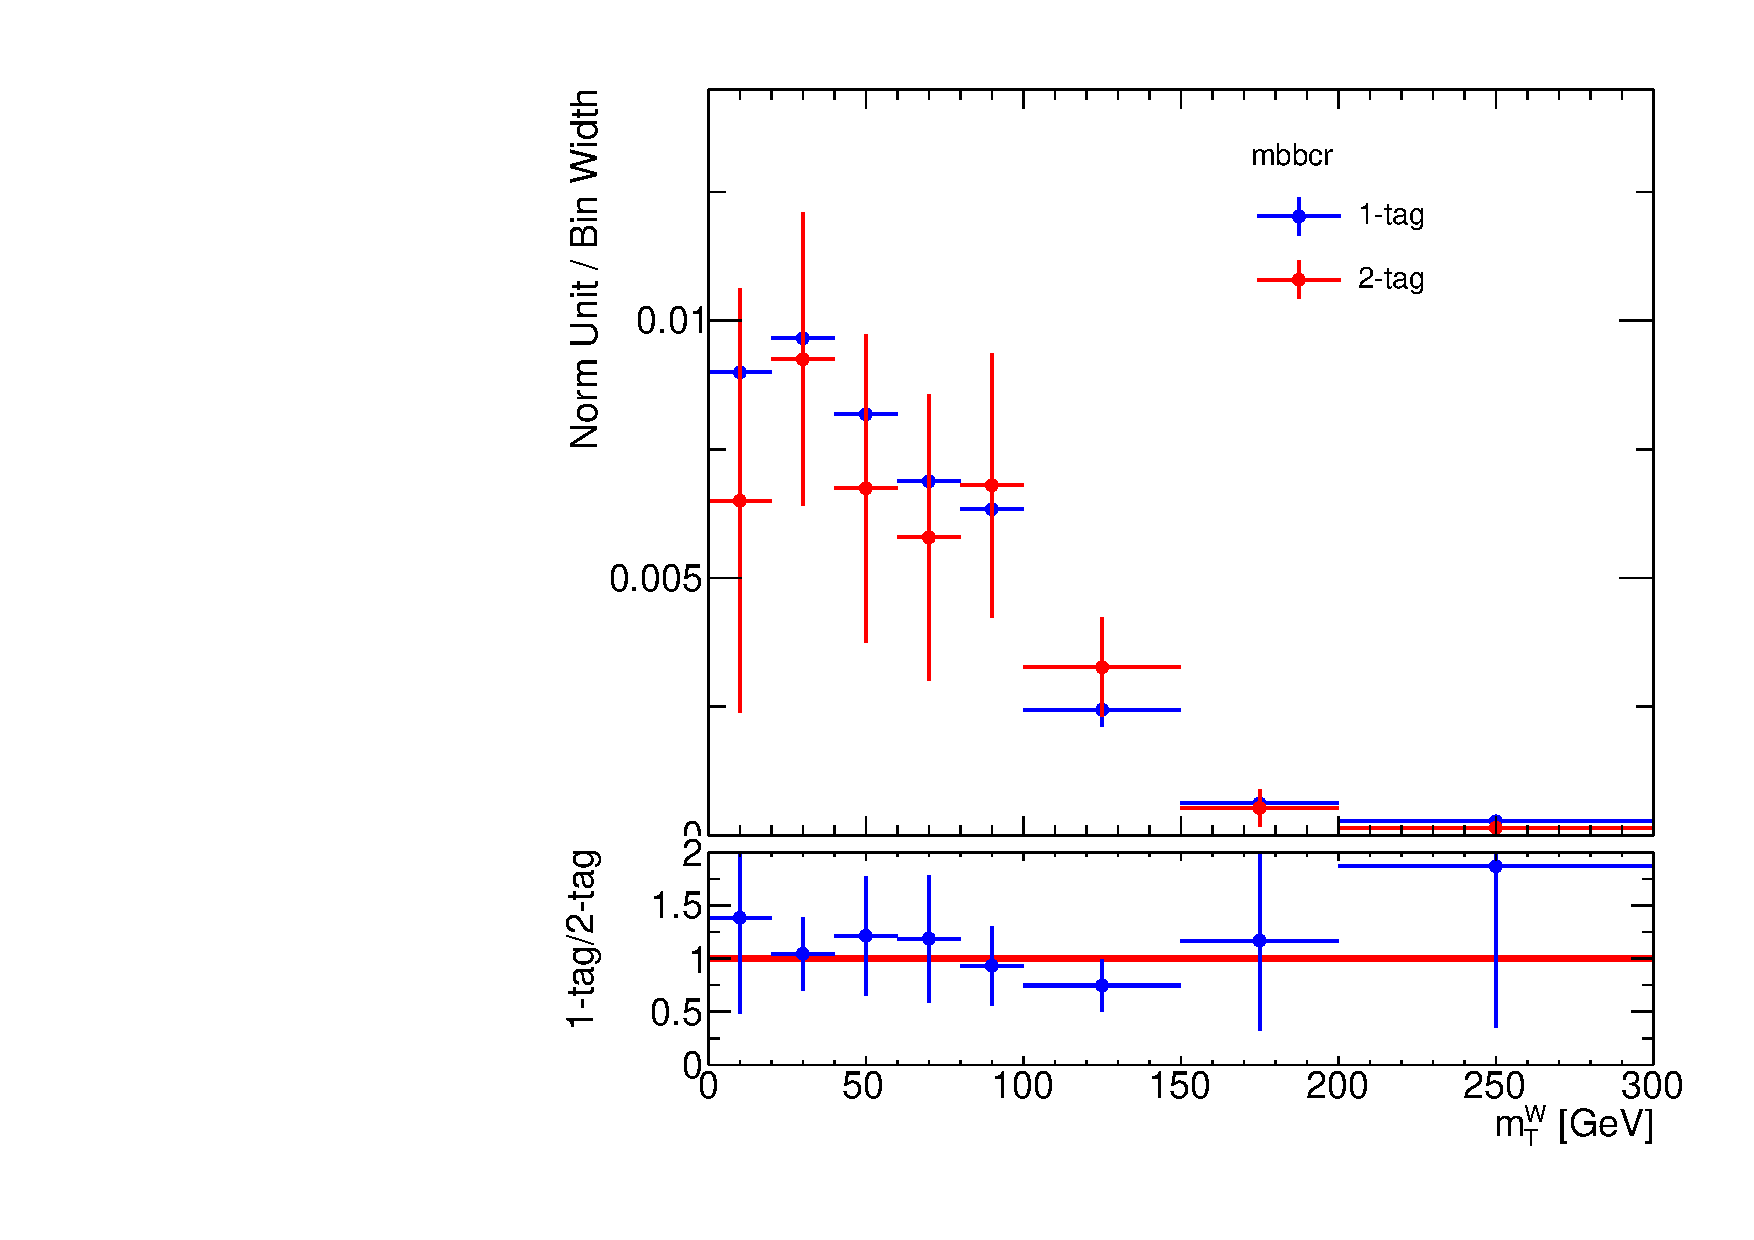
\includegraphics[scale=0.33]{./figures/boosted/ABCD/ABCD_2TagVs1Tag_mbbcr_lepton_WlepMtATLAS}\\
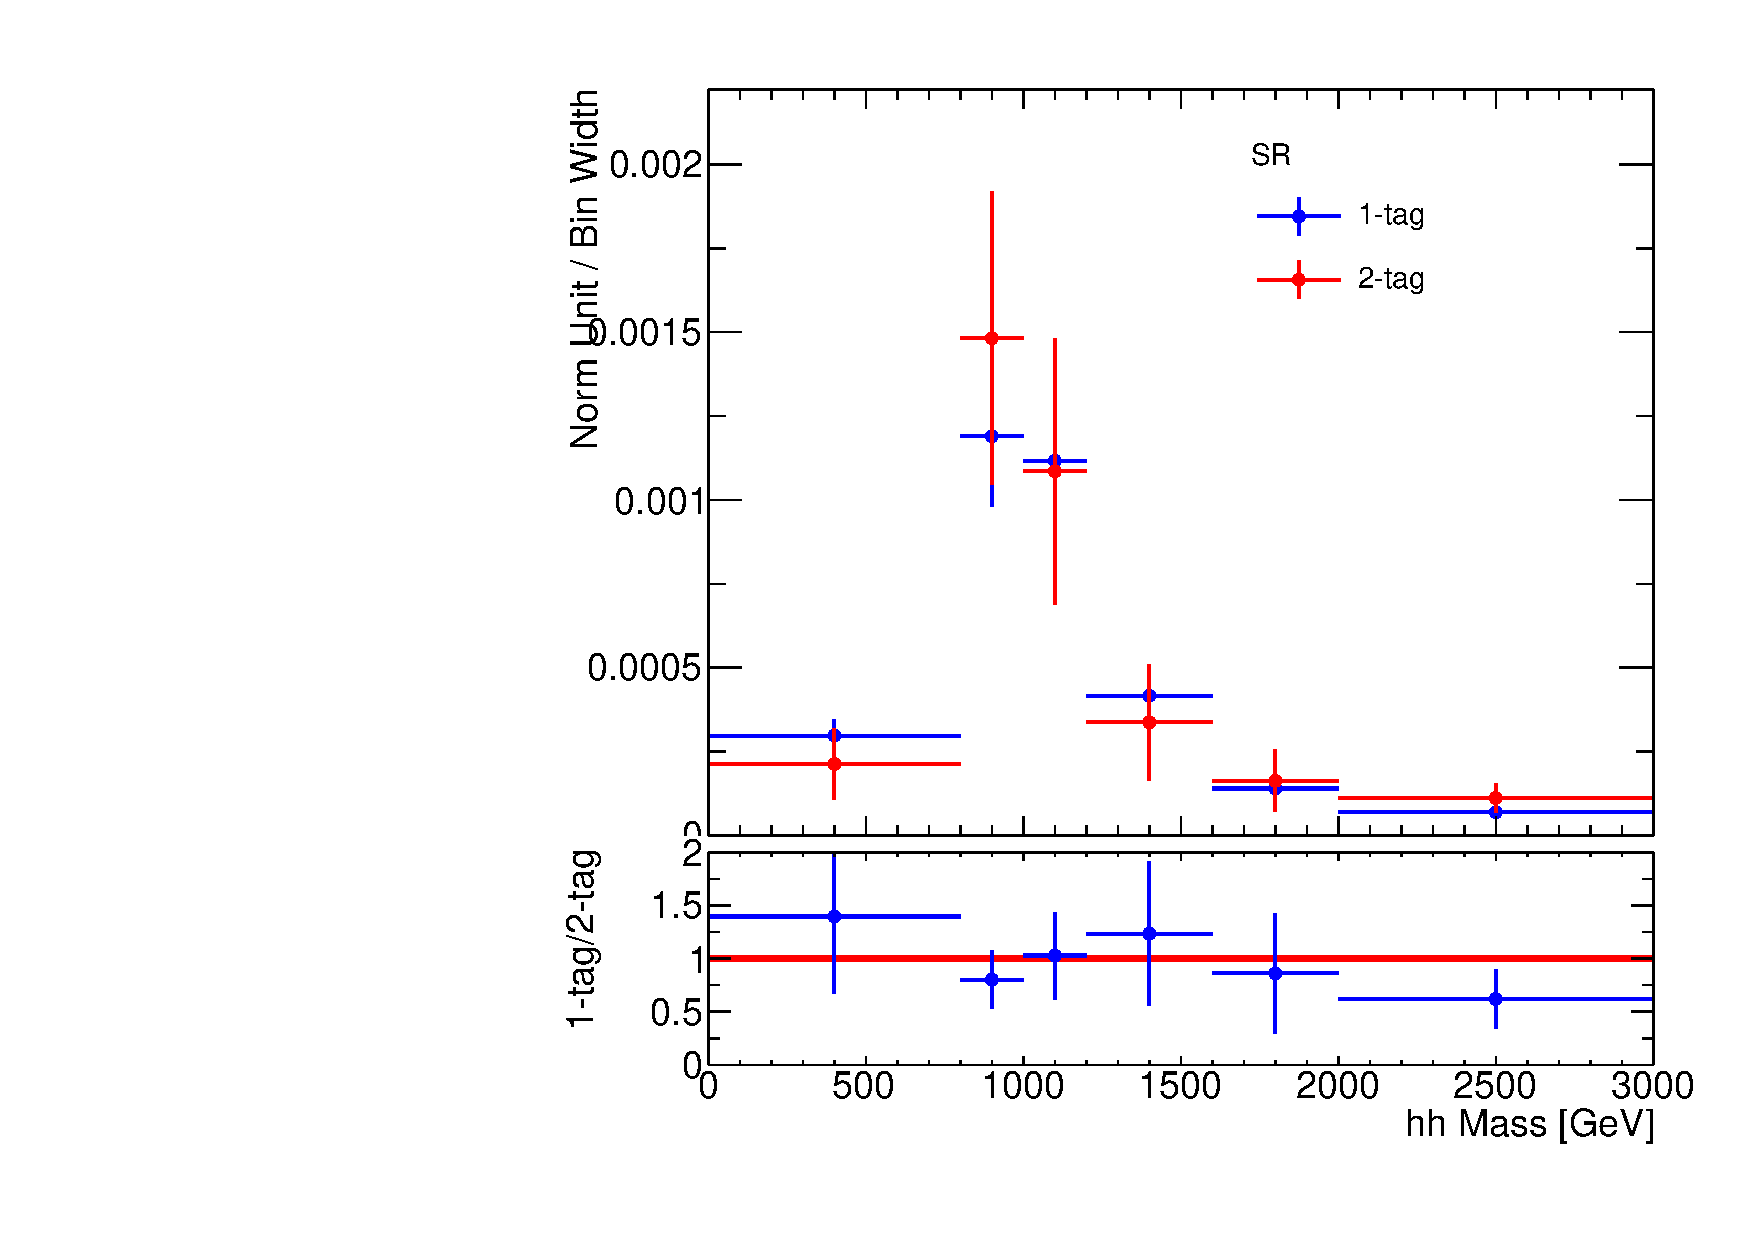
\includegraphics[scale=0.33]{./figures/boosted/ABCD/ABCD_2TagVs1Tag_SR_lepton_hhMass}    
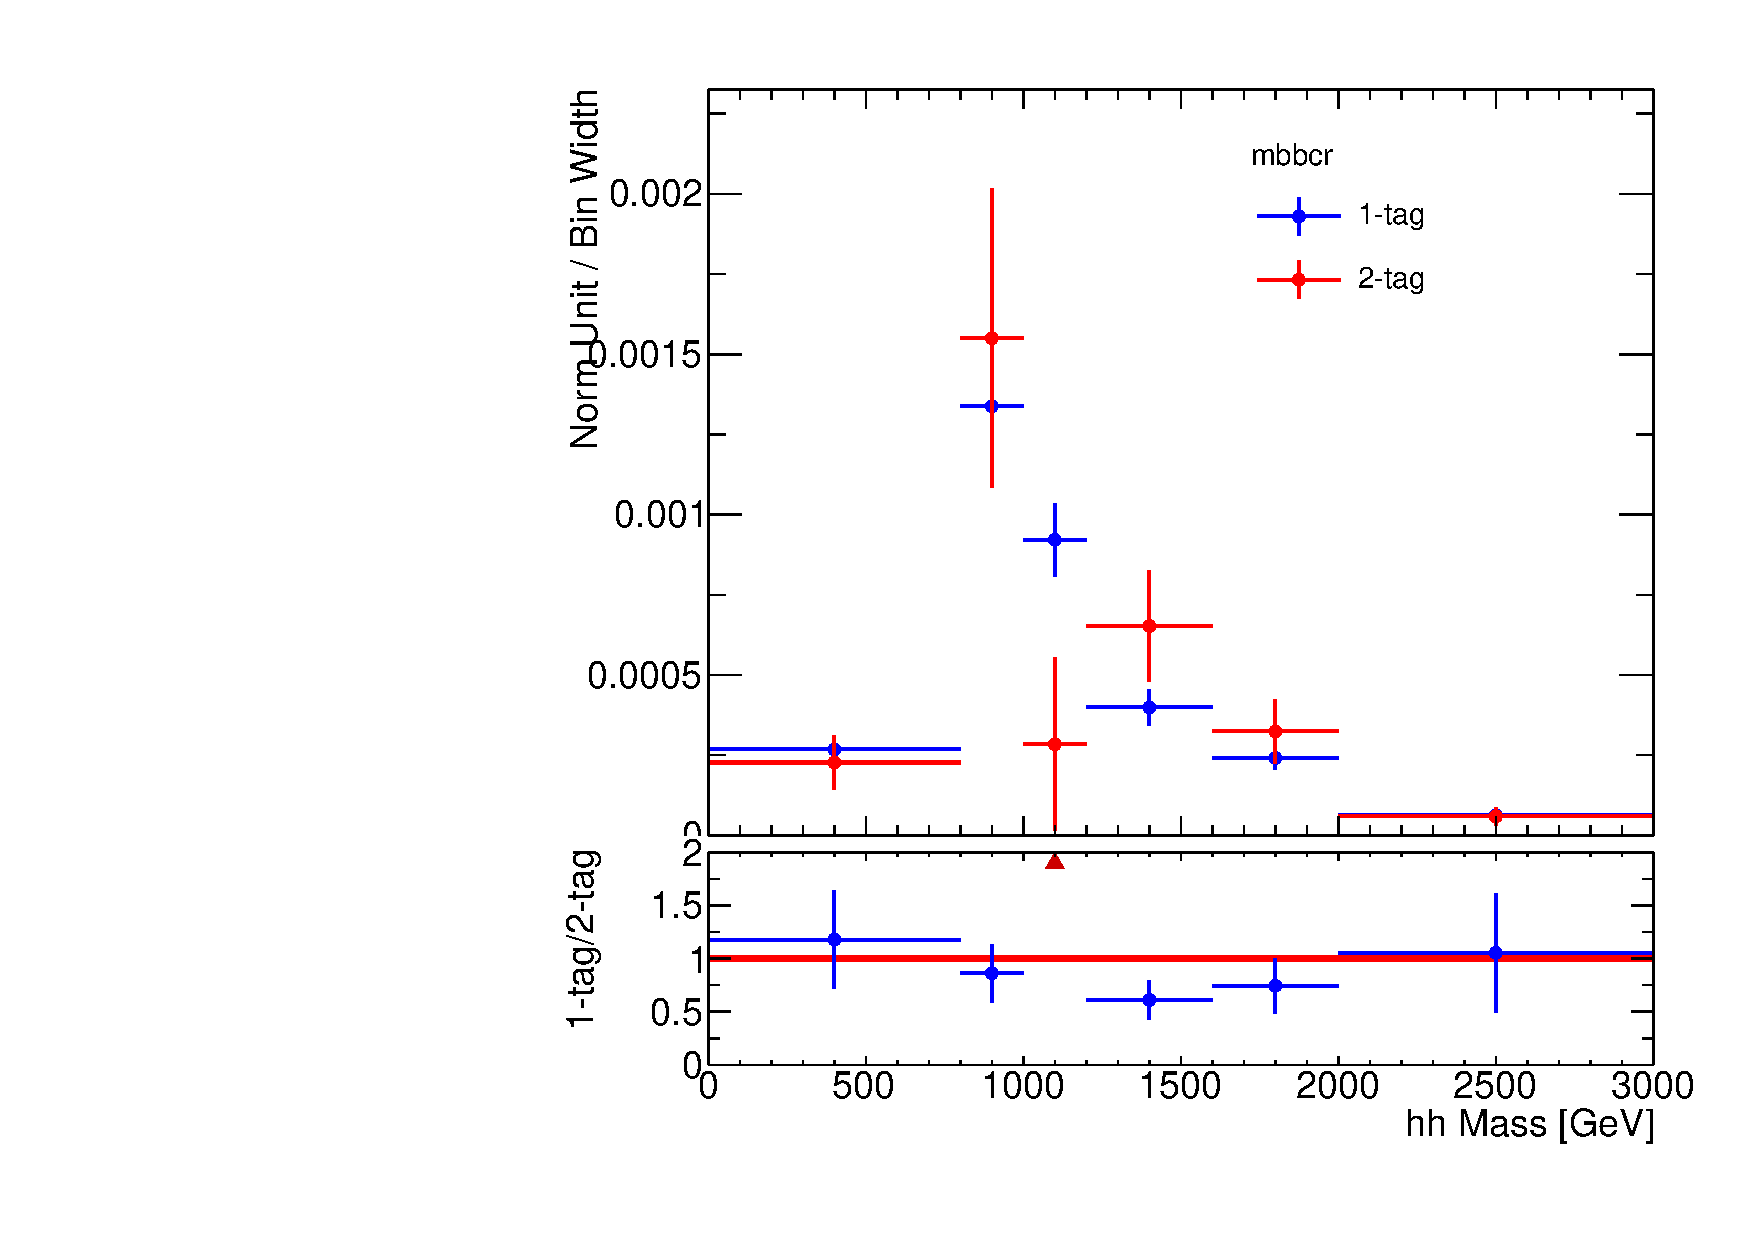
\includegraphics[scale=0.33]{./figures/boosted/ABCD/ABCD_2TagVs1Tag_mbbcr_lepton_hhMass} 
\caption{Comparisons of the qcd multijet template kinematic distributions between 1-tag (black) and 2-tag (red) events 
in region C. Plots on the left are in the signal region while on the right are in mBB control region. All distributions
are normalized to the same area. The error bars represent the statistical uncertainty of the templates.}
\label{fig:boosted_abcd_2tag1tag}
\end{center}
\end{figure}

\FloatBarrier
%%%%%%%%%%%%%%%%%%%%%%%%
%
% Region B and D distributions
%
%%%%%%%%%%%%%%%%%%%%%%%
\subsection{Region B and Region D distributions}
\label{app:boosted_qcd_region_bd}

Figure~\ref{fig:boosted_abcd_region_bd_muon} and~\ref{fig:boosted_abcd_region_bd_elec} show several kinematic distributions
in region B and region D for the muon channel and electron channel respectively.

\begin{figure}[!htbp]
\begin{center}
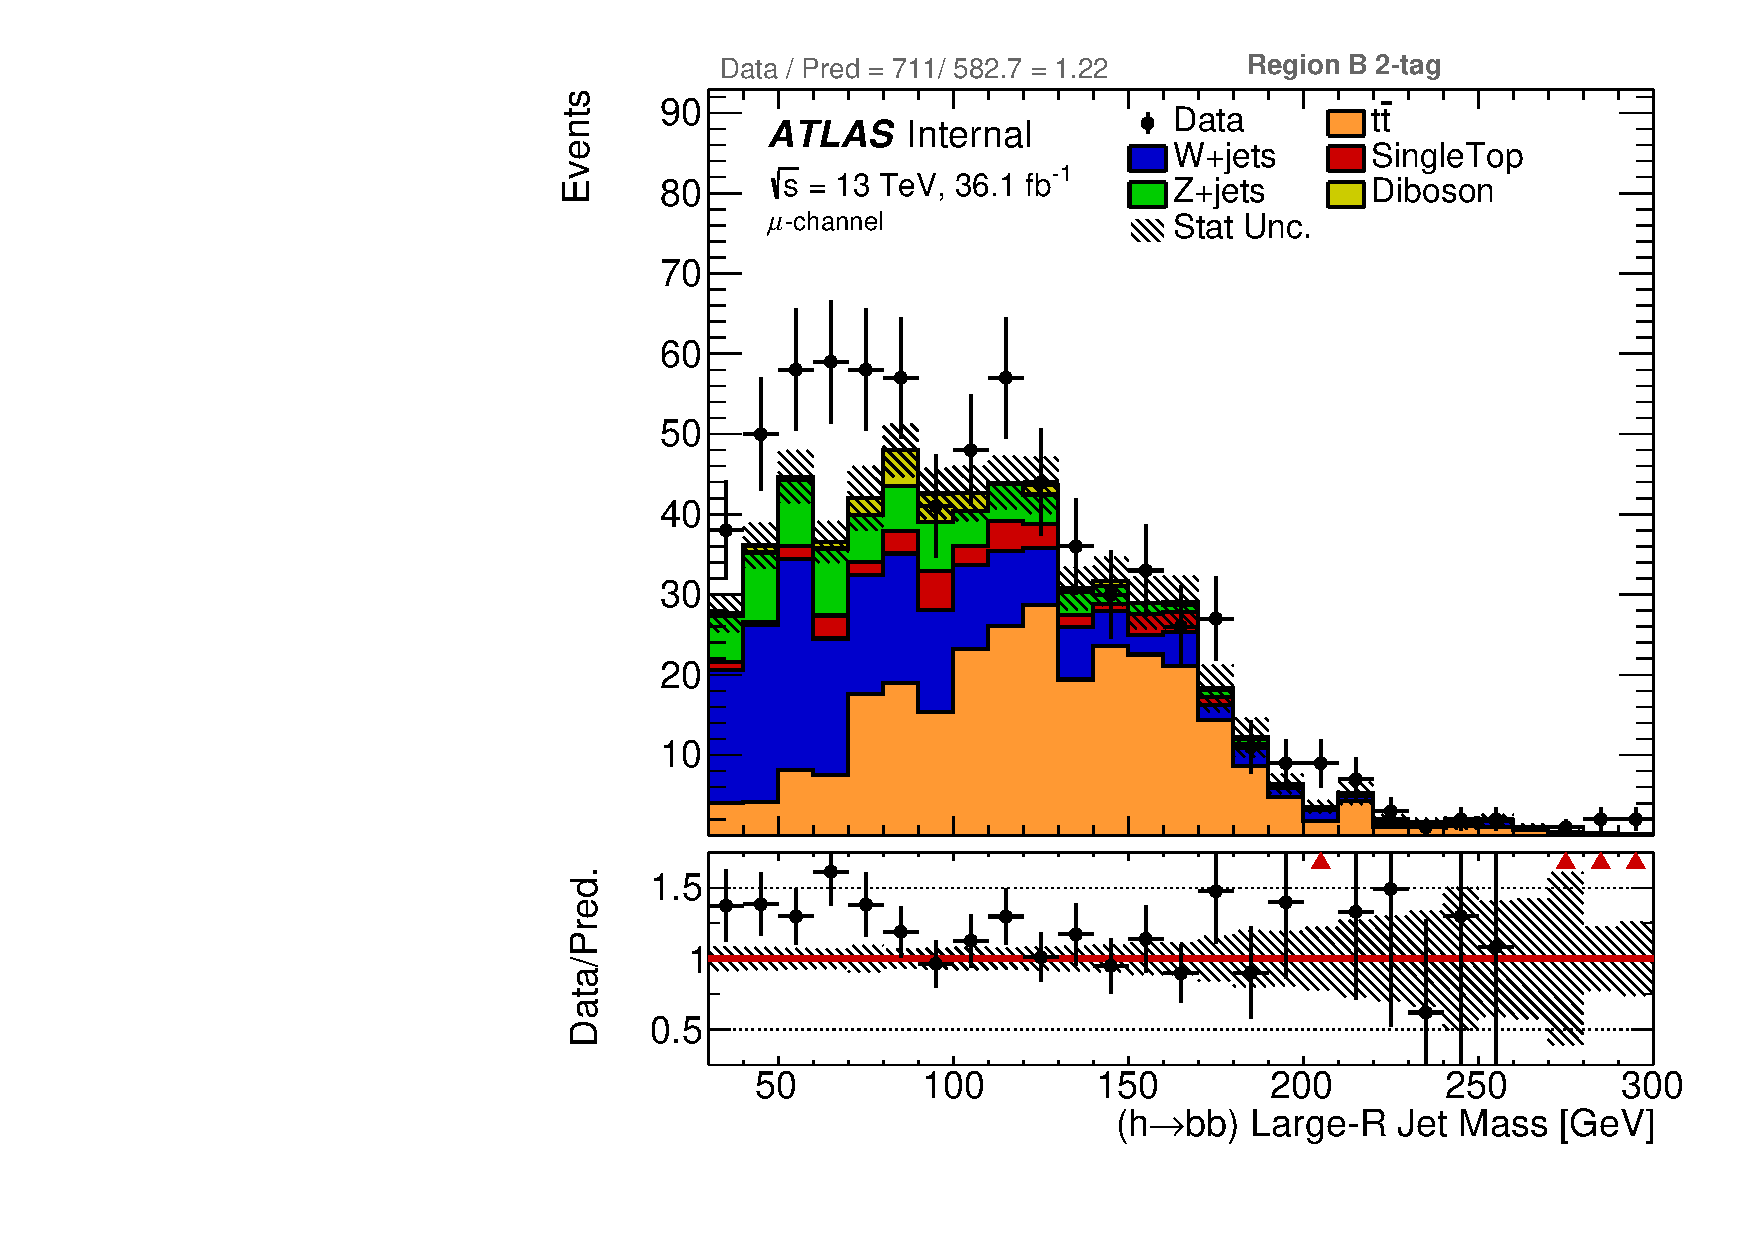
\includegraphics[scale=0.23]{./figures/boosted/ABCD/muon_Inc_RegionB_HbbMass}
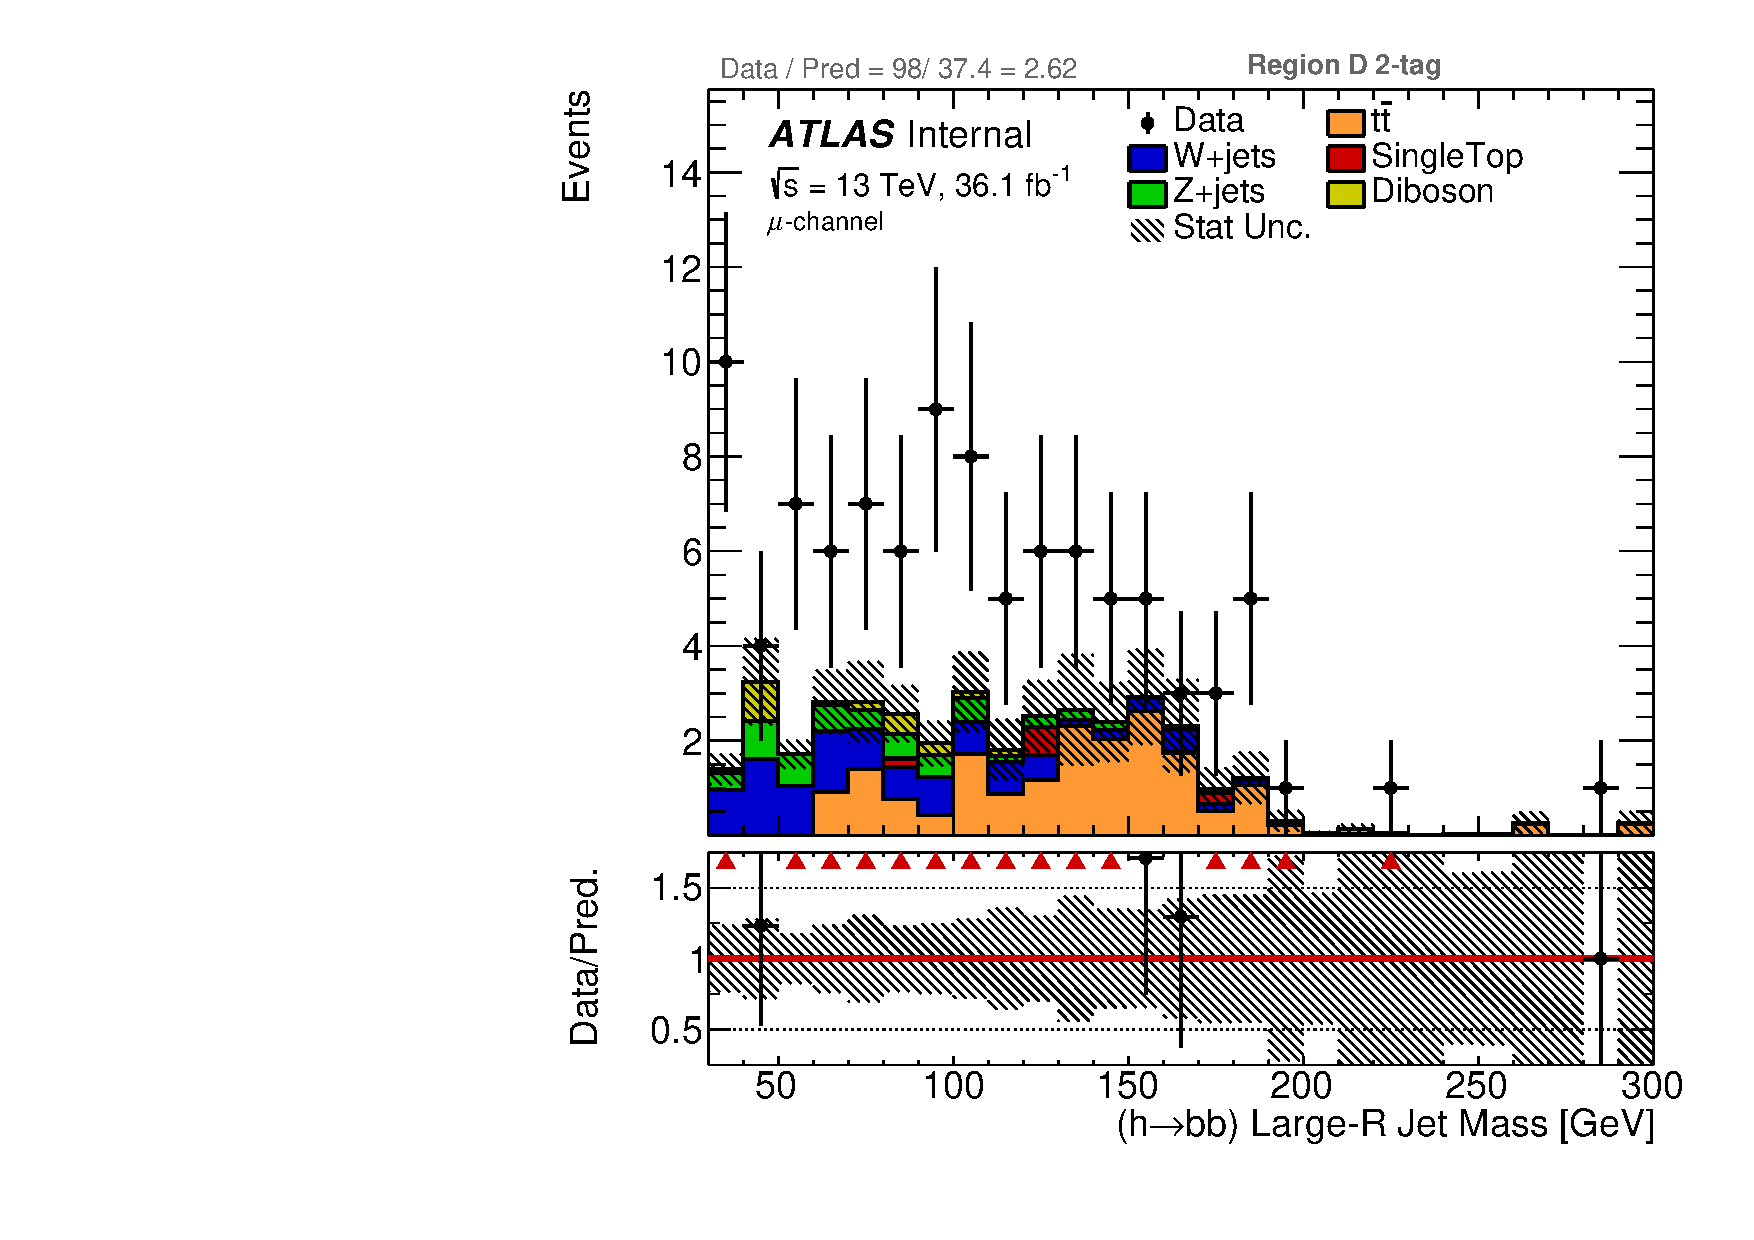
\includegraphics[scale=0.23]{./figures/boosted/ABCD/muon_Inc_RegionD_HbbMass}\\
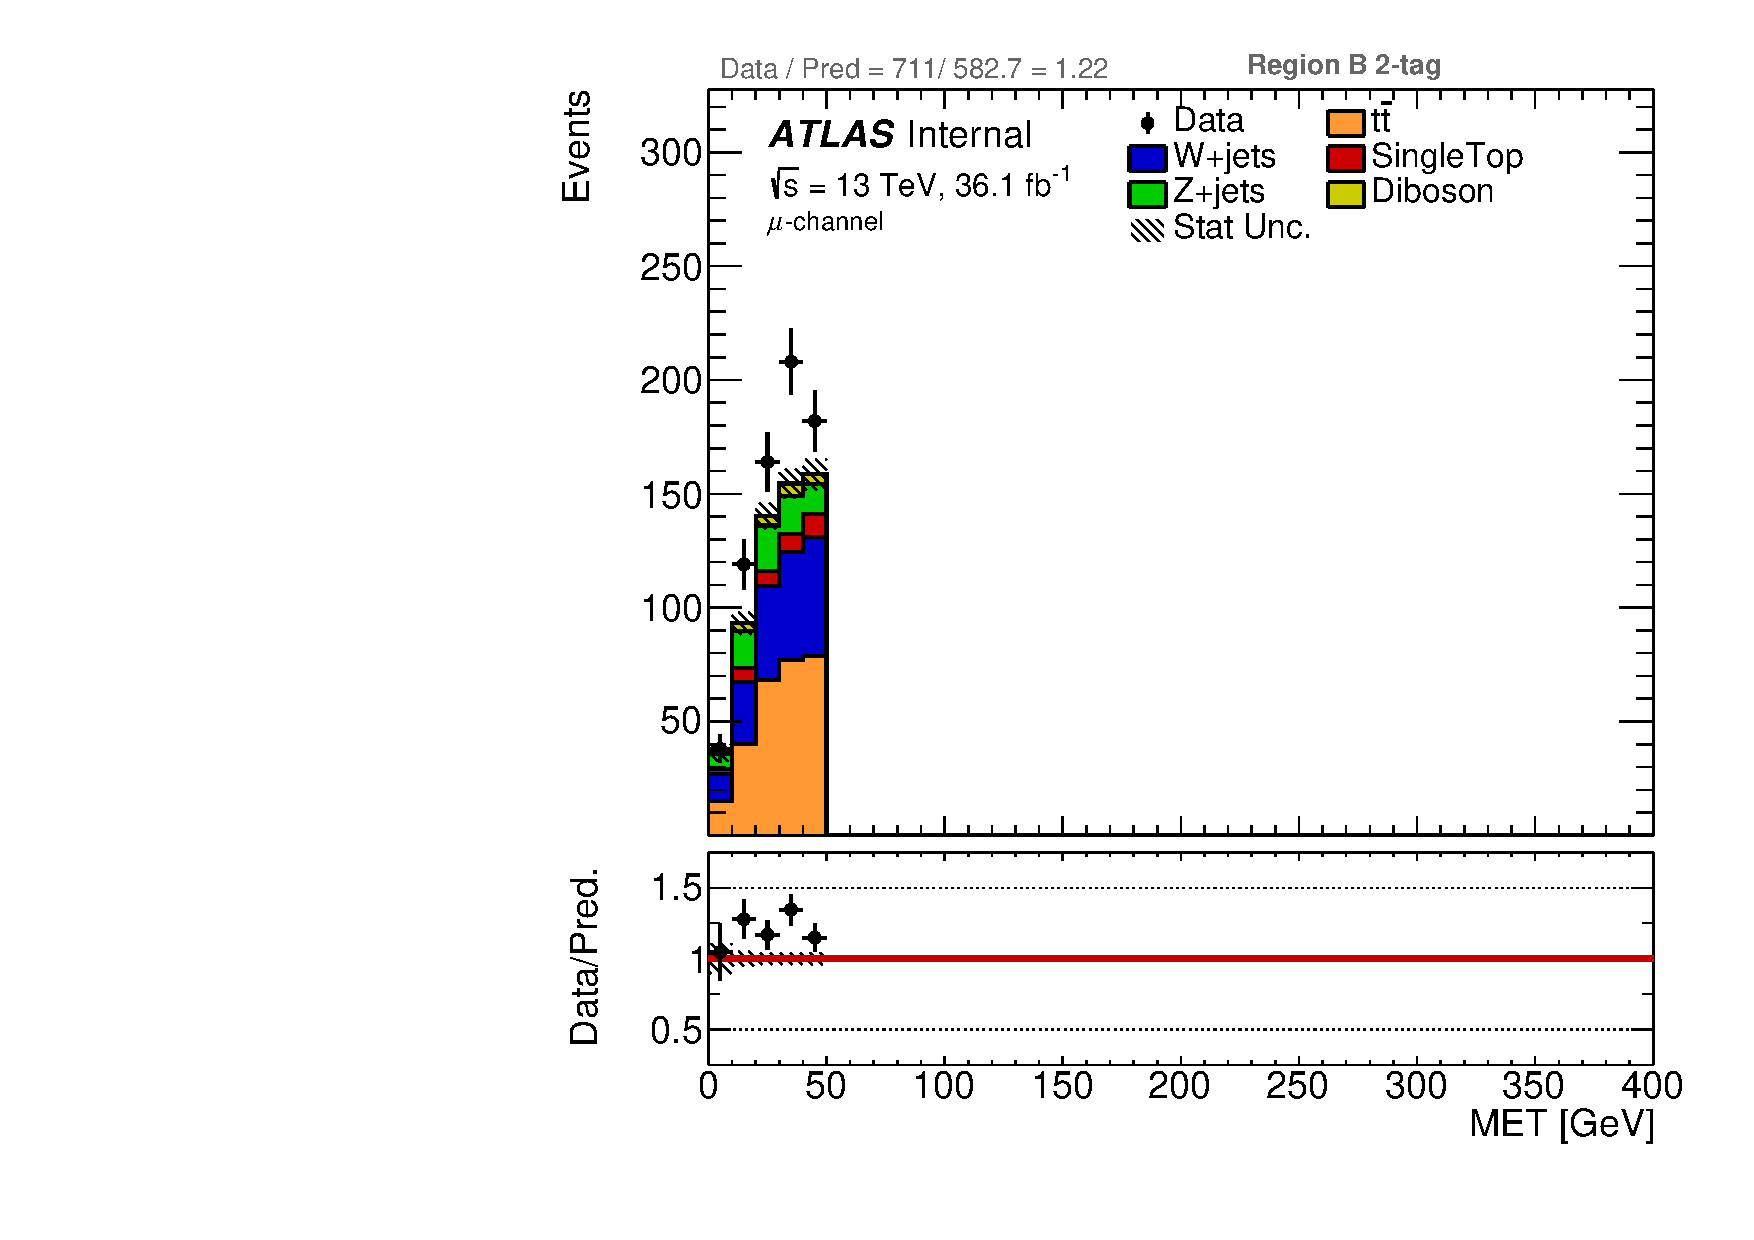
\includegraphics[scale=0.23]{./figures/boosted/ABCD/muon_Inc_RegionB_MET}
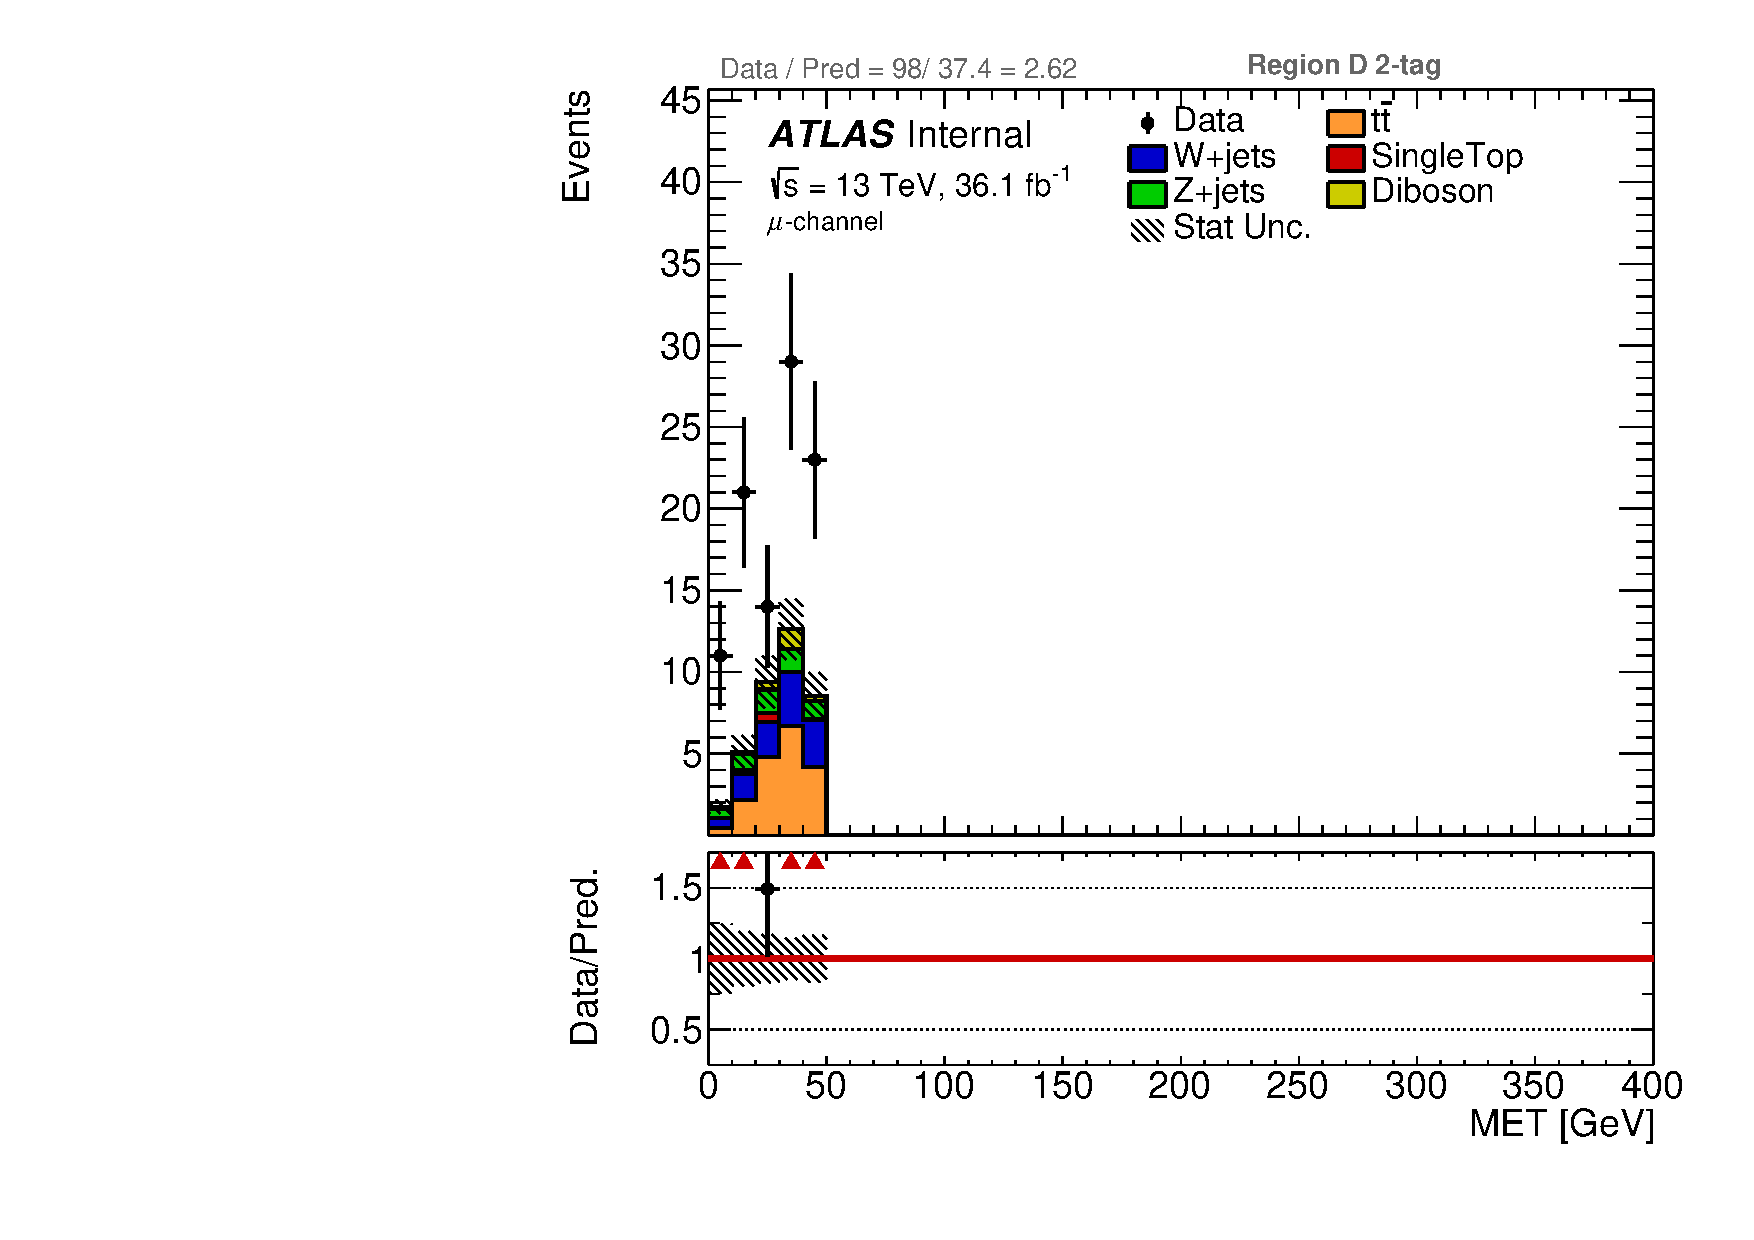
\includegraphics[scale=0.23]{./figures/boosted/ABCD/muon_Inc_RegionD_MET}\\
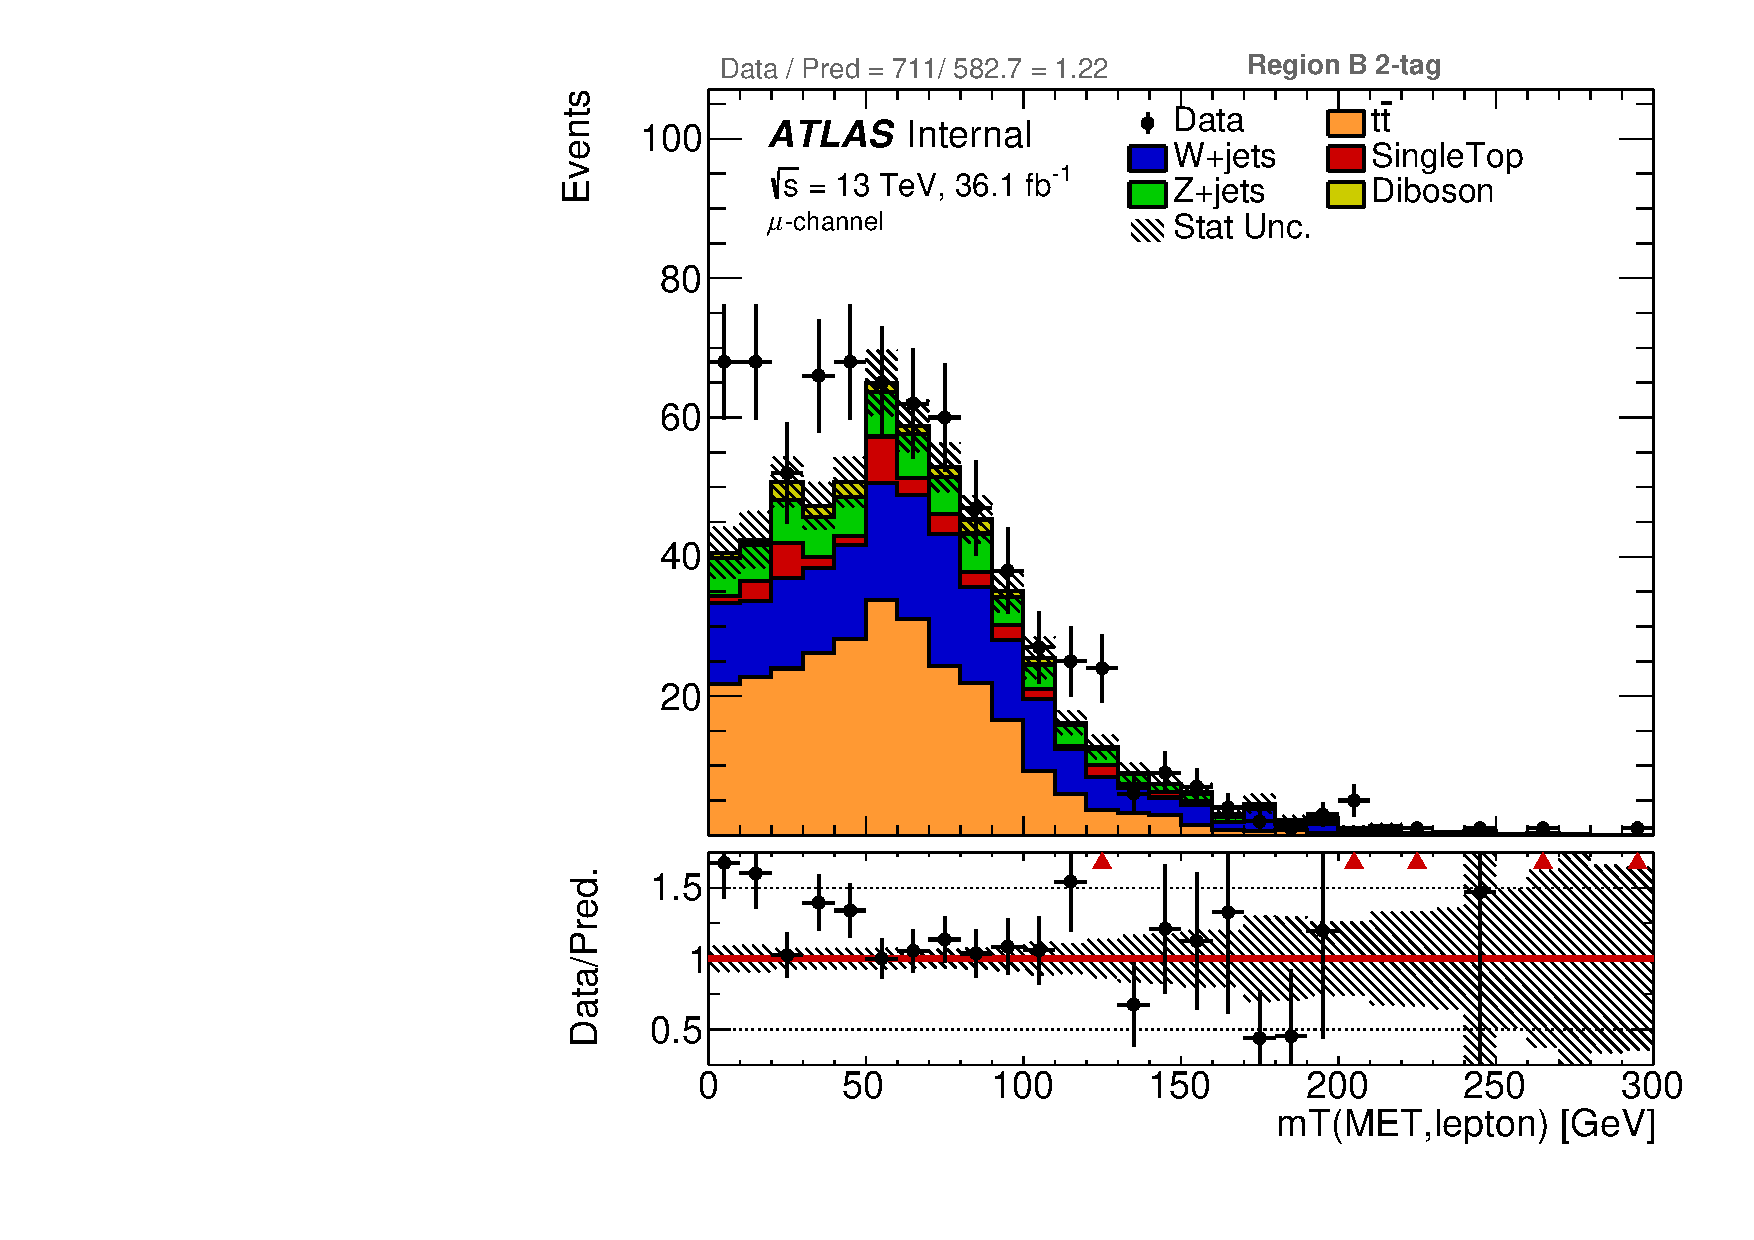
\includegraphics[scale=0.23]{./figures/boosted/ABCD/muon_Inc_RegionB_WlepMtATLAS}
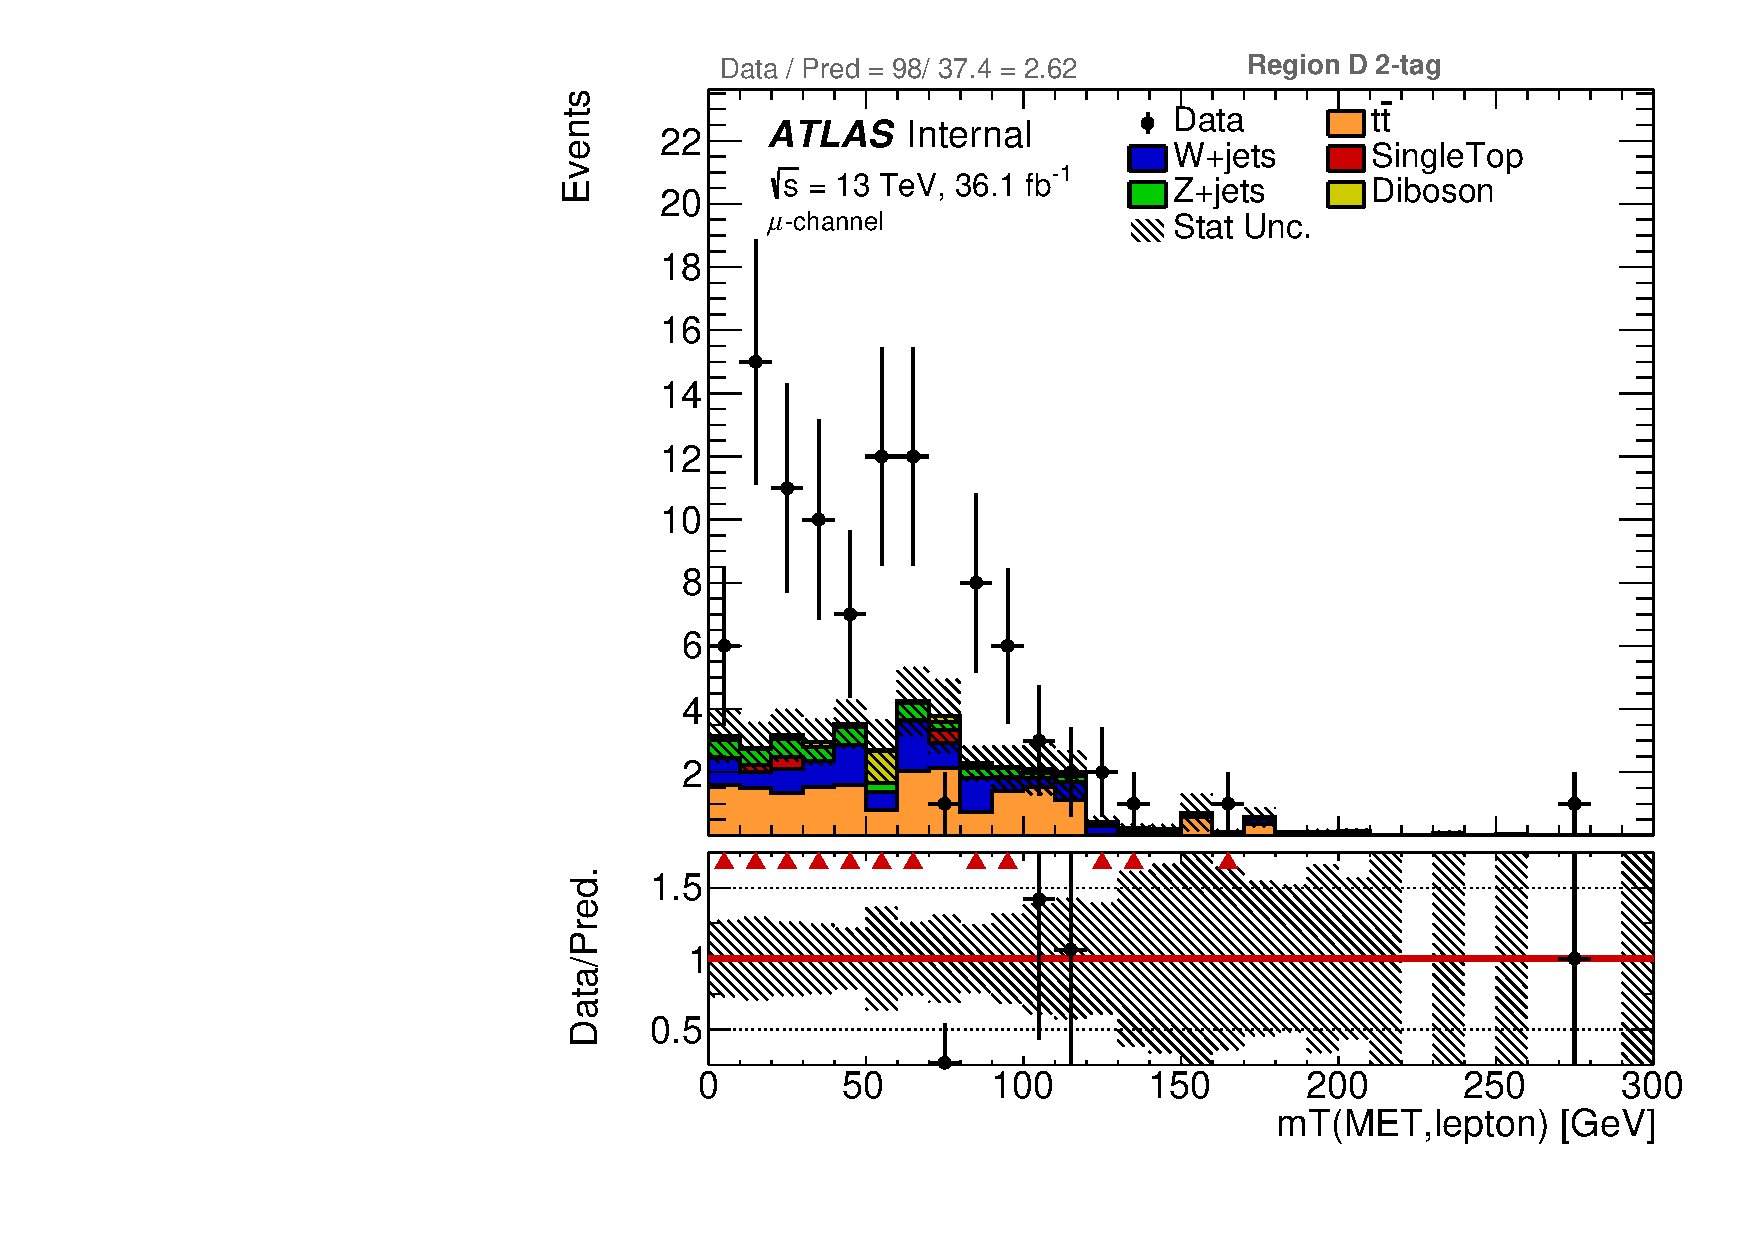
\includegraphics[scale=0.23]{./figures/boosted/ABCD/muon_Inc_RegionD_WlepMtATLAS}\\
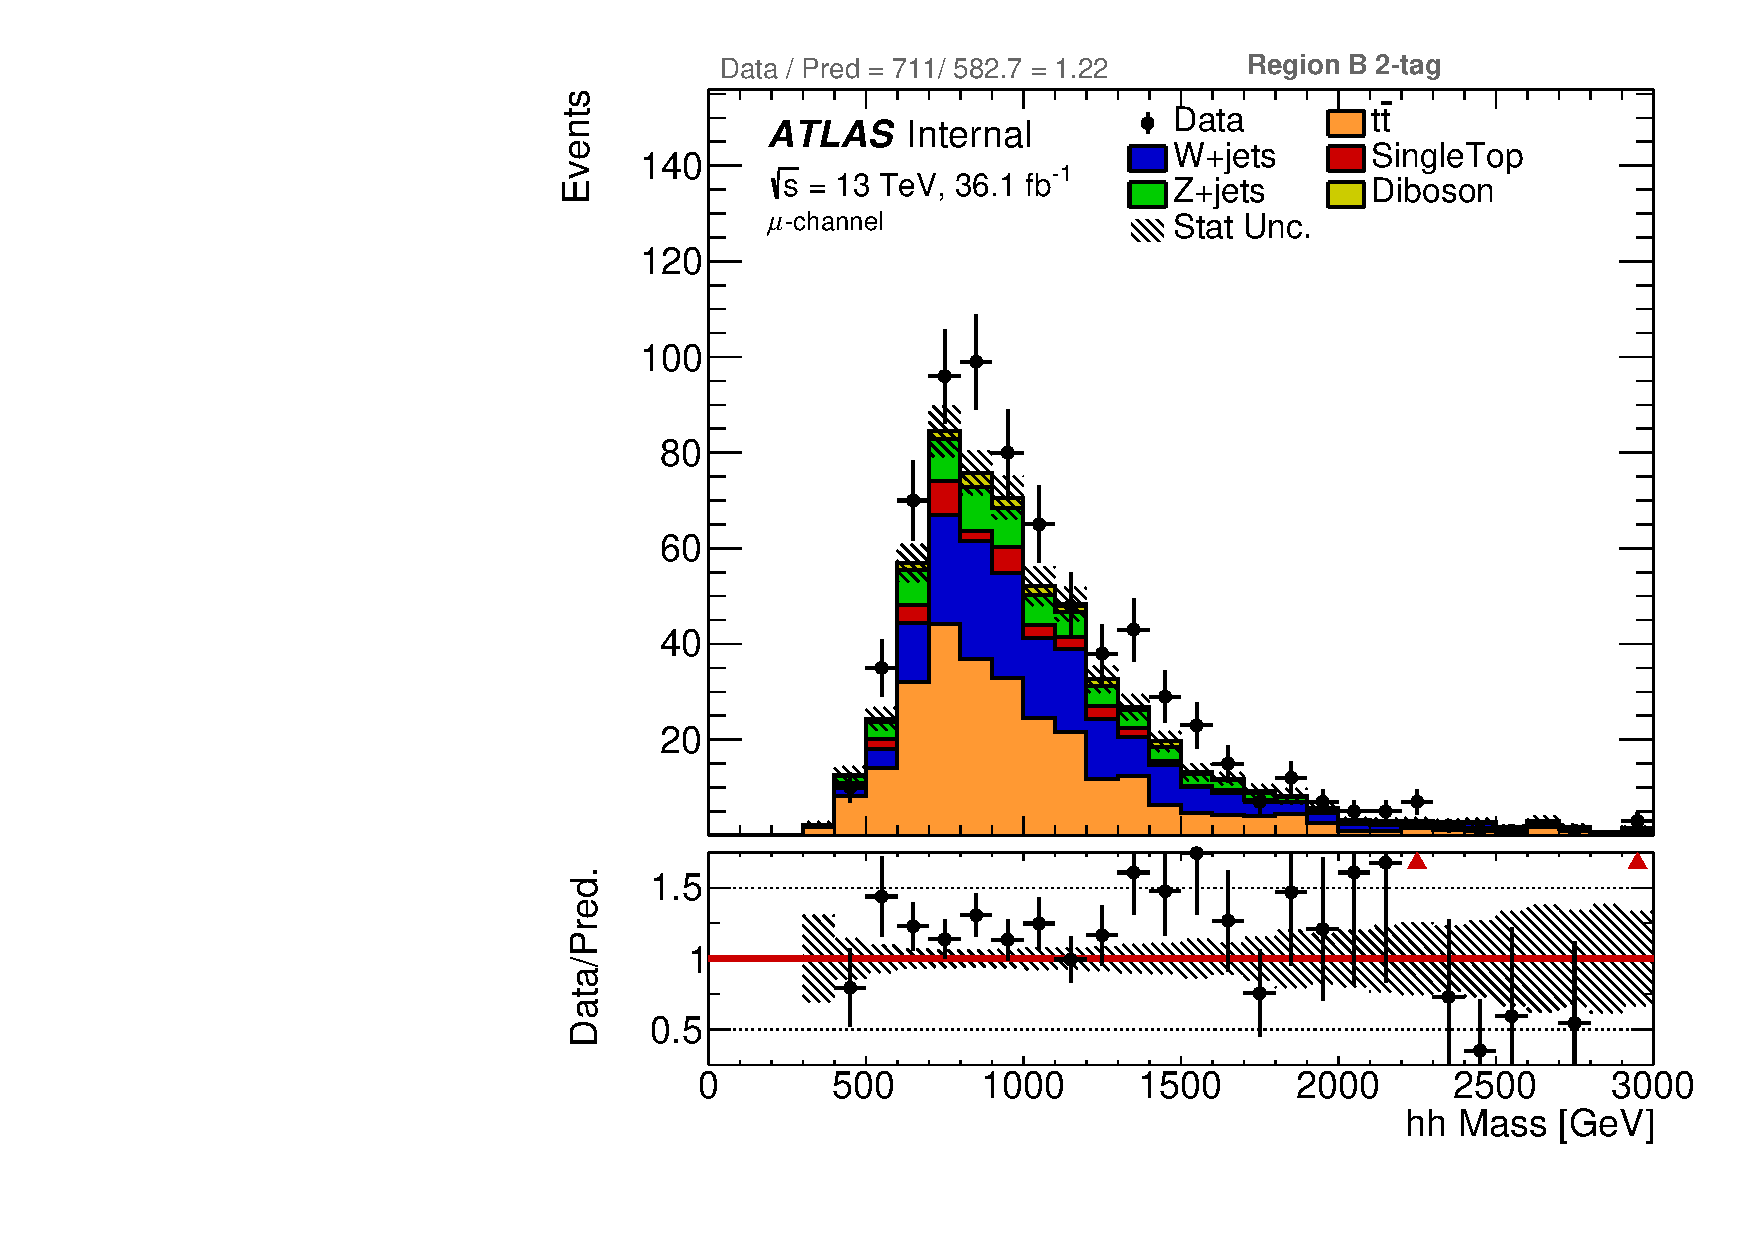
\includegraphics[scale=0.23]{./figures/boosted/ABCD/muon_Inc_RegionB_hhMass}
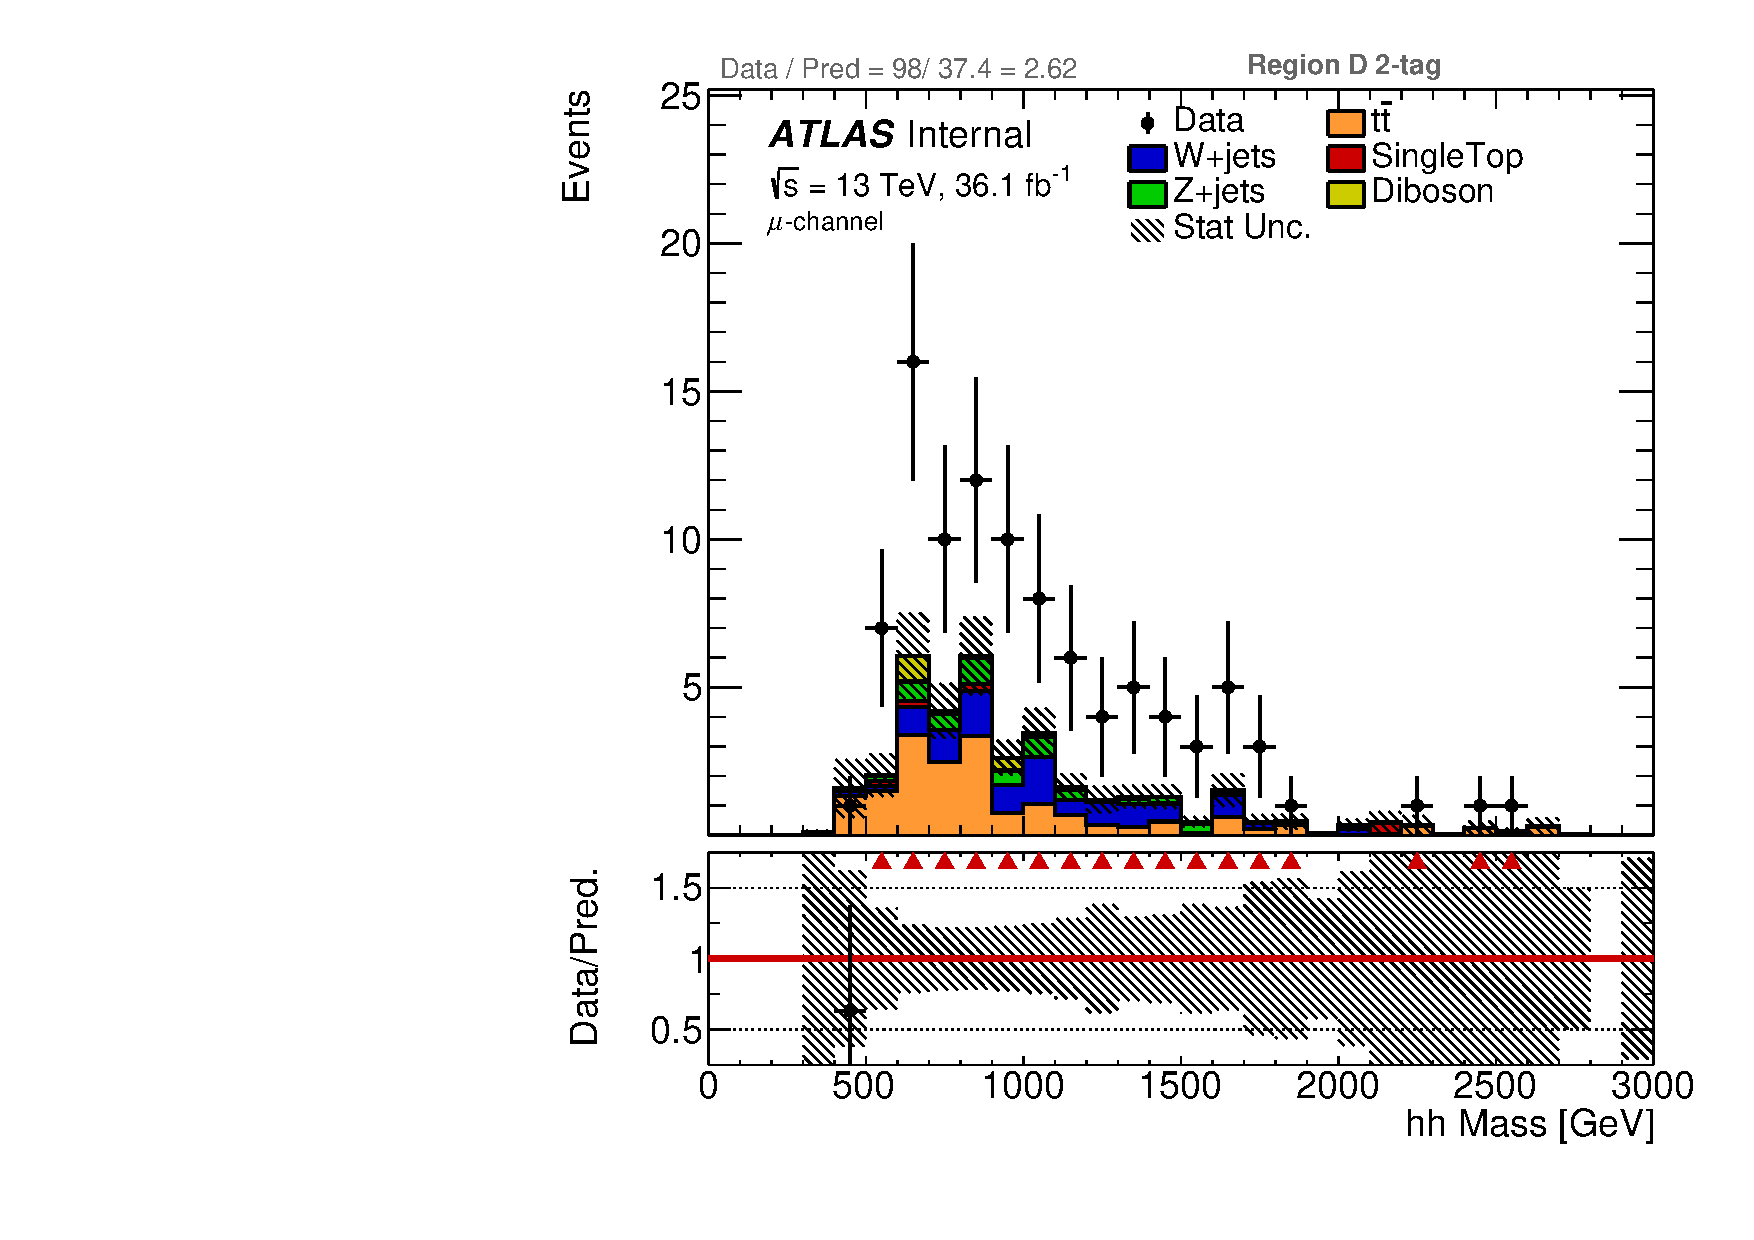
\includegraphics[scale=0.23]{./figures/boosted/ABCD/muon_Inc_RegionD_hhMass}
\caption{Kinematic distributions in ABCD method region B (left) and region D (right) in the muon channel.}
\label{fig:boosted_abcd_region_bd_muon}
\end{center}
\end{figure}


\begin{figure}[!htbp]
\begin{center}
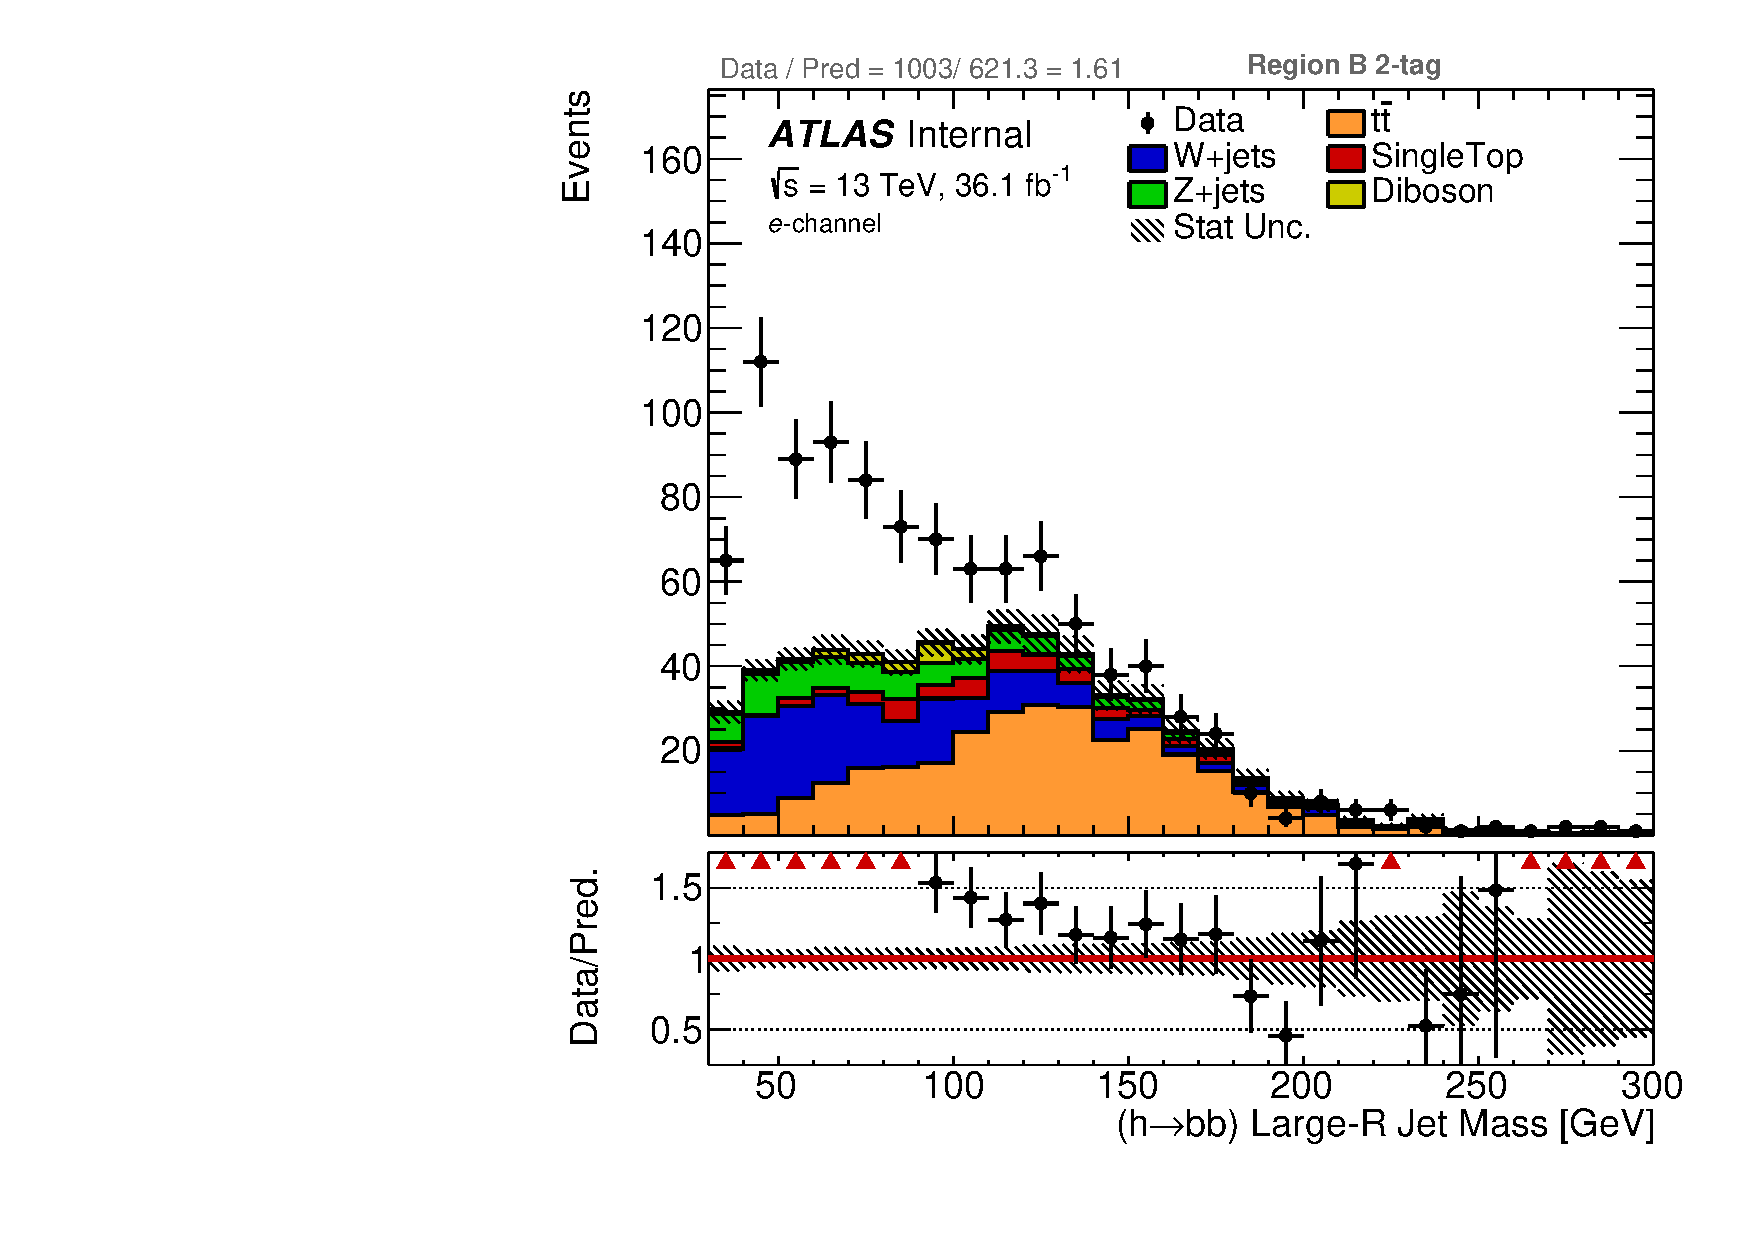
\includegraphics[scale=0.23]{./figures/boosted/ABCD/elec_Inc_RegionB_HbbMass}
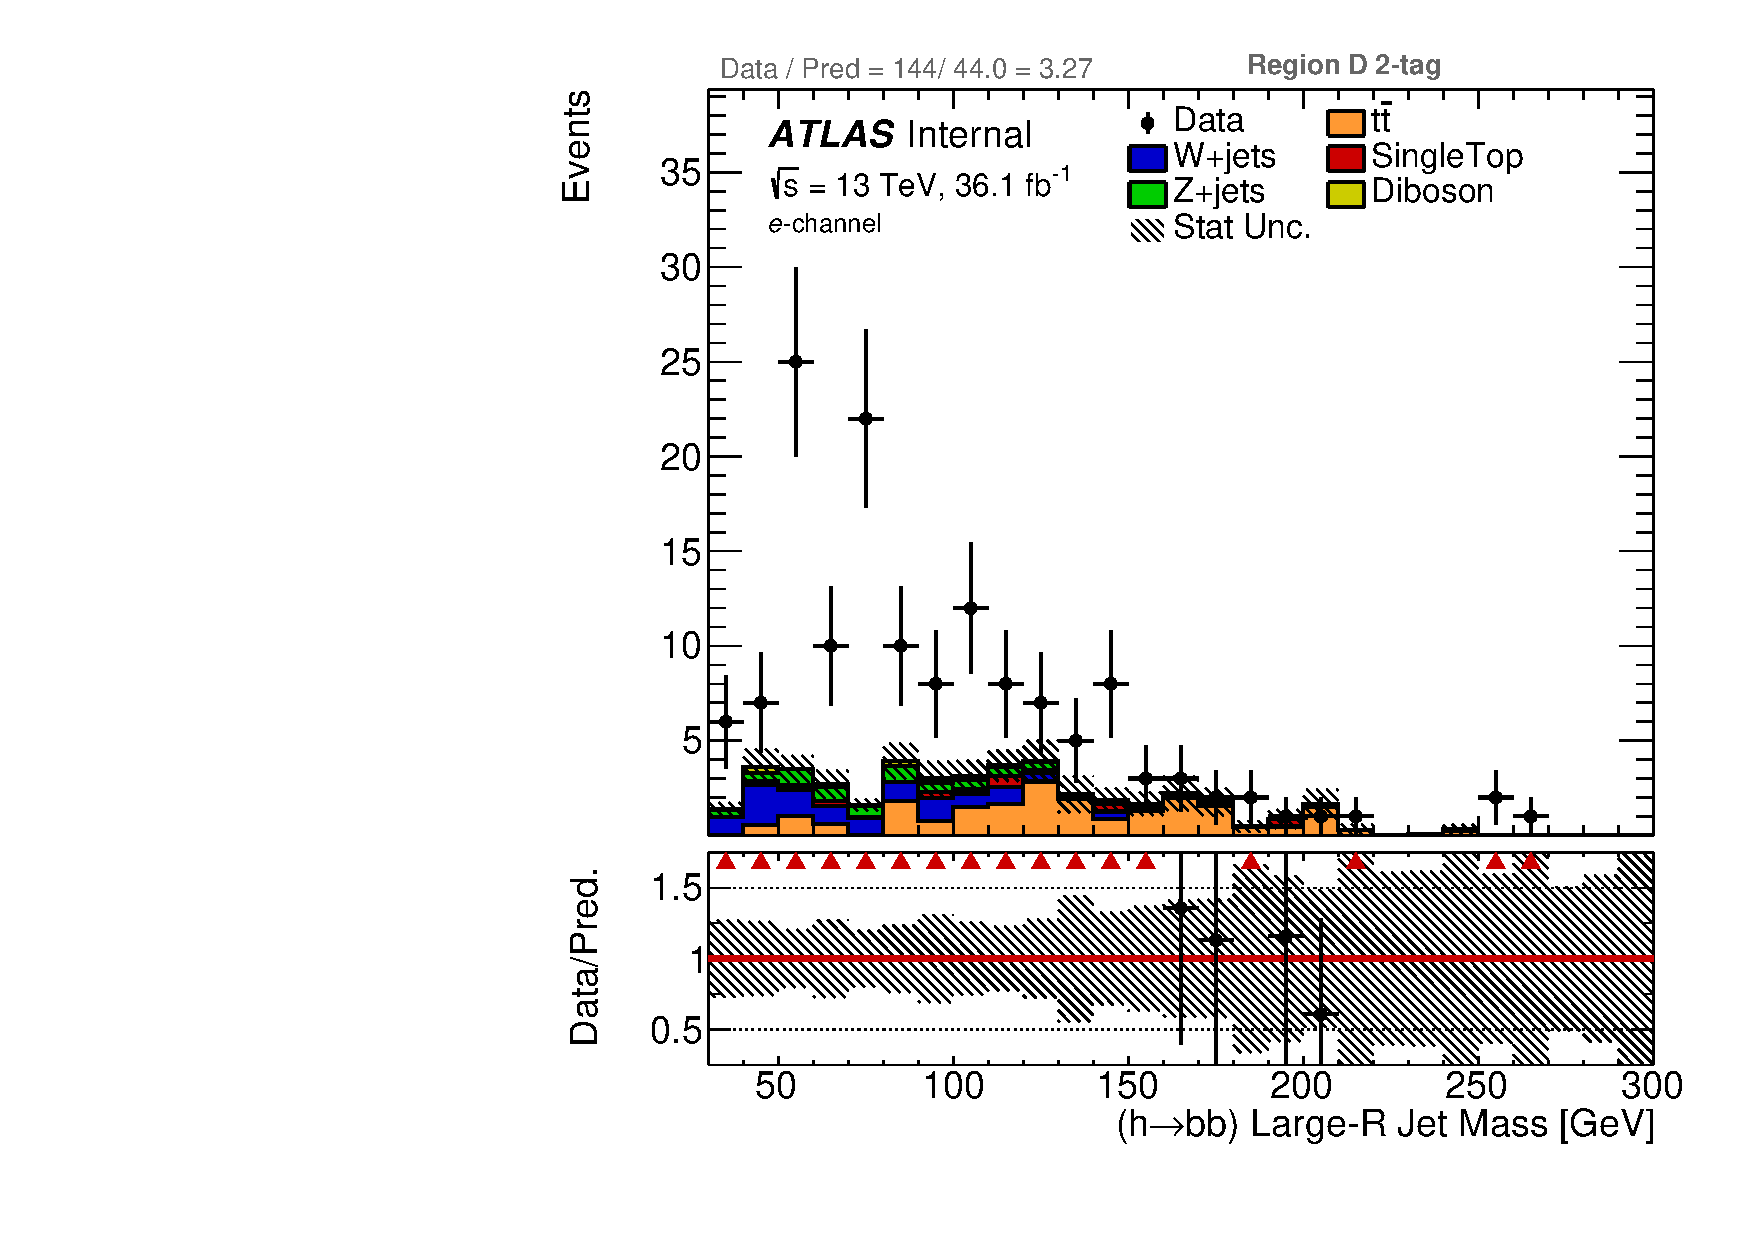
\includegraphics[scale=0.23]{./figures/boosted/ABCD/elec_Inc_RegionD_HbbMass}\\
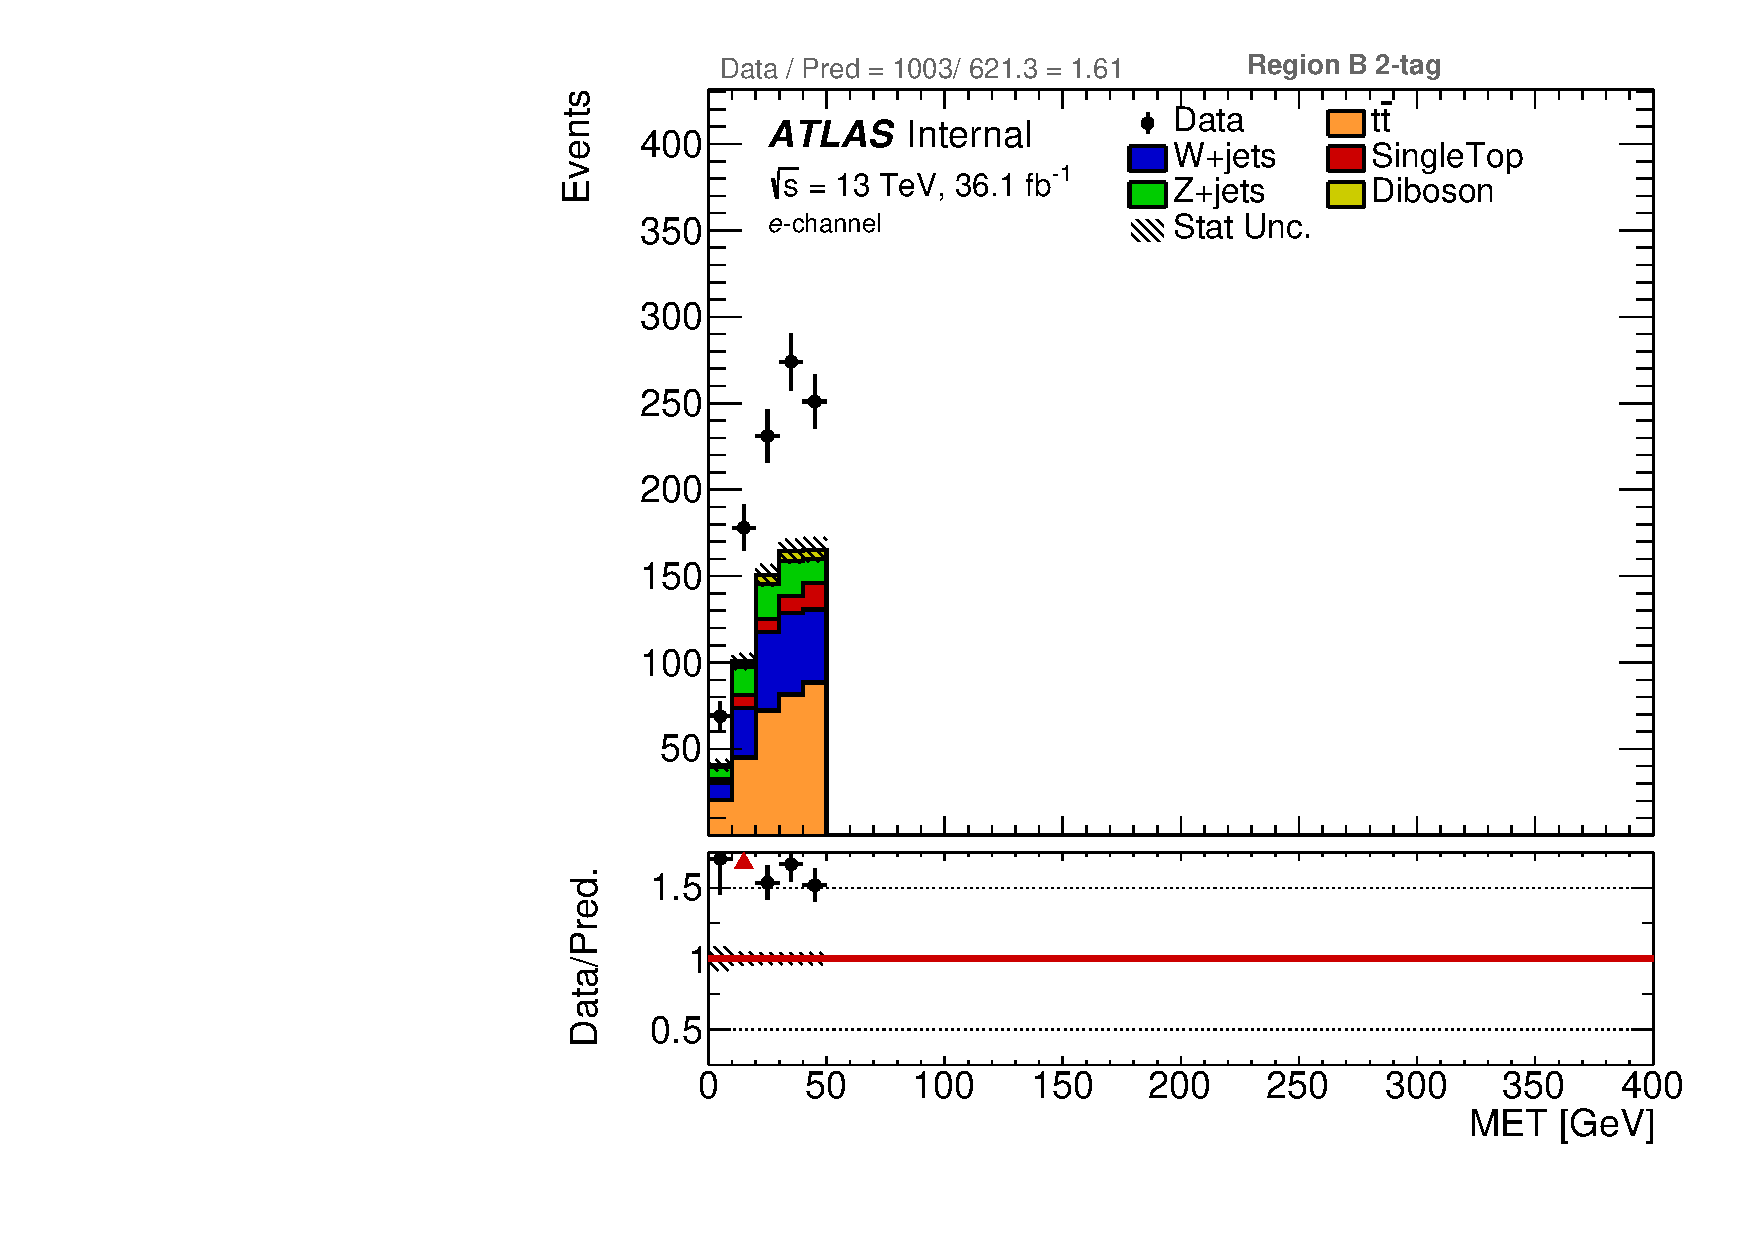
\includegraphics[scale=0.23]{./figures/boosted/ABCD/elec_Inc_RegionB_MET}
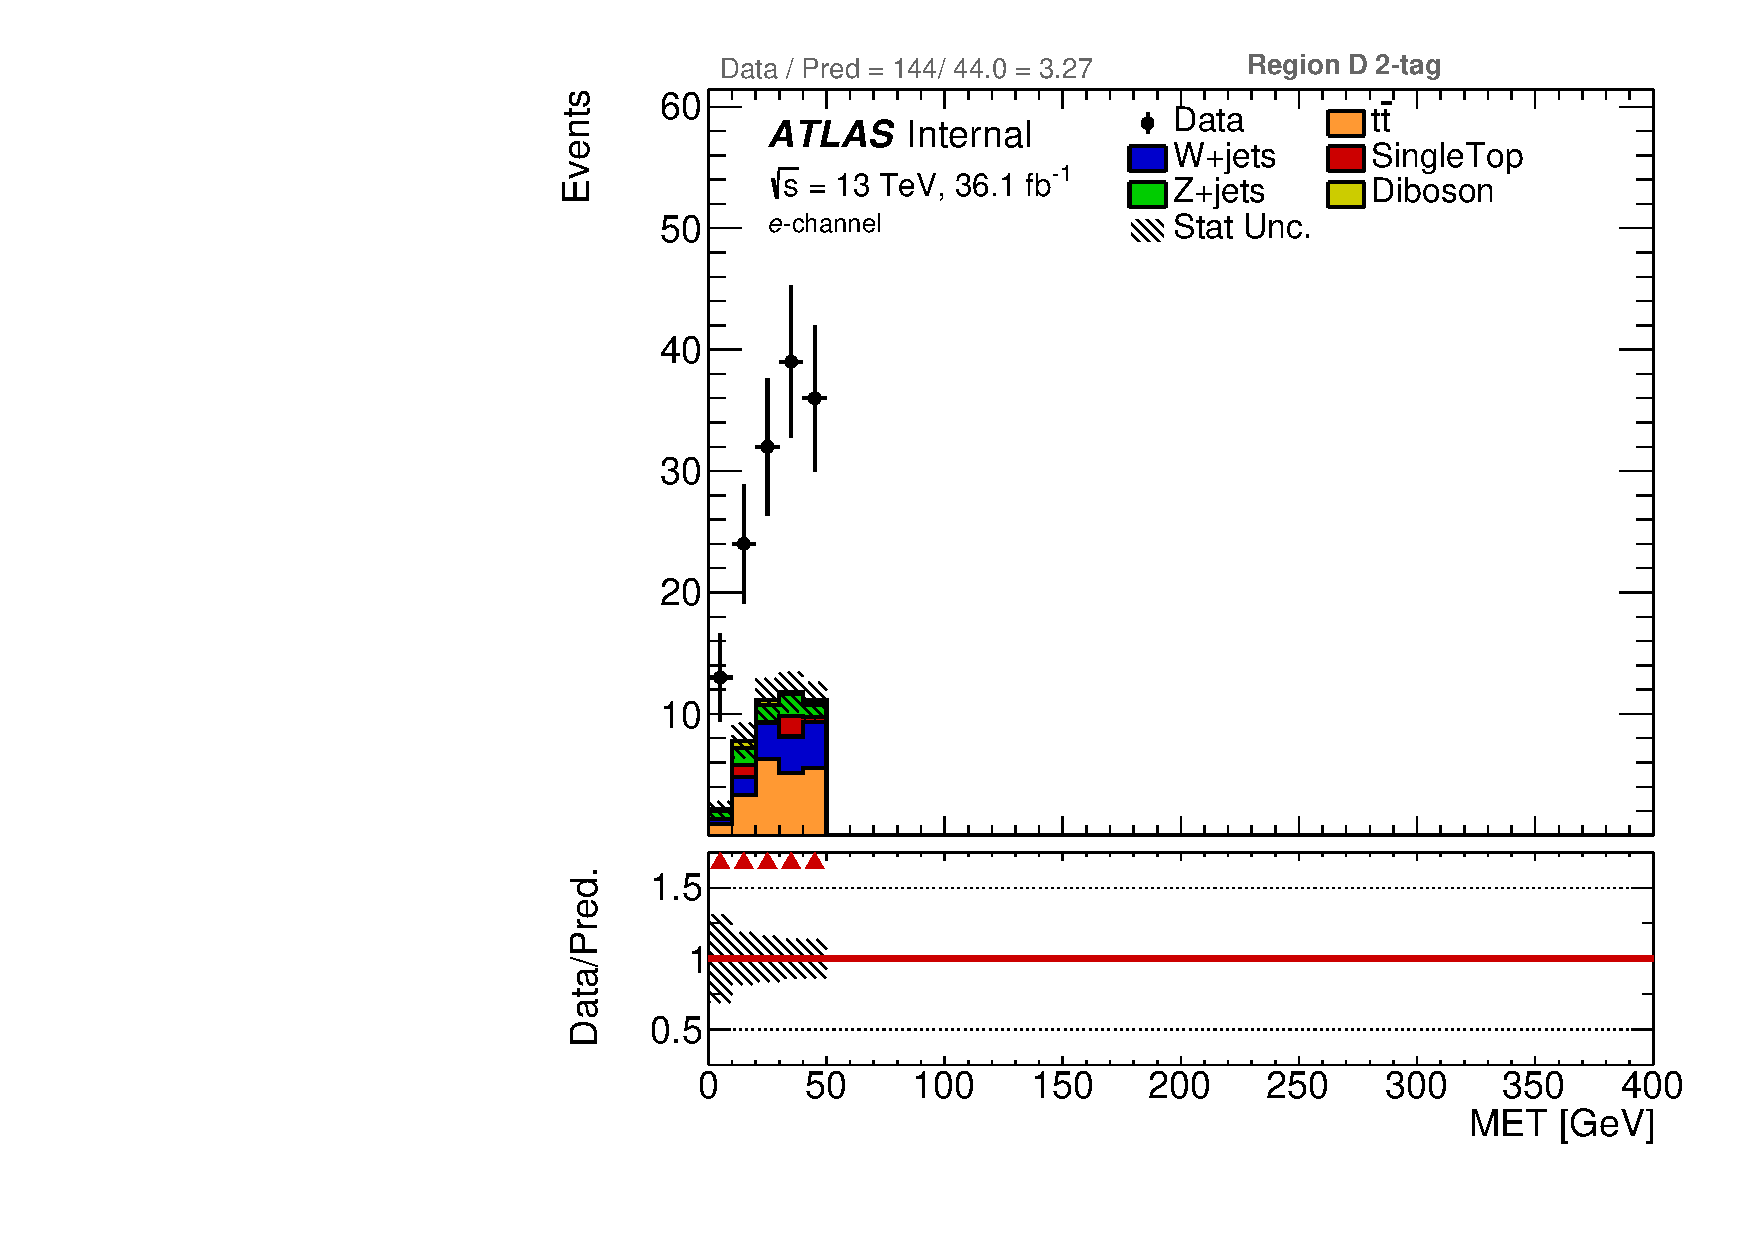
\includegraphics[scale=0.23]{./figures/boosted/ABCD/elec_Inc_RegionD_MET}\\
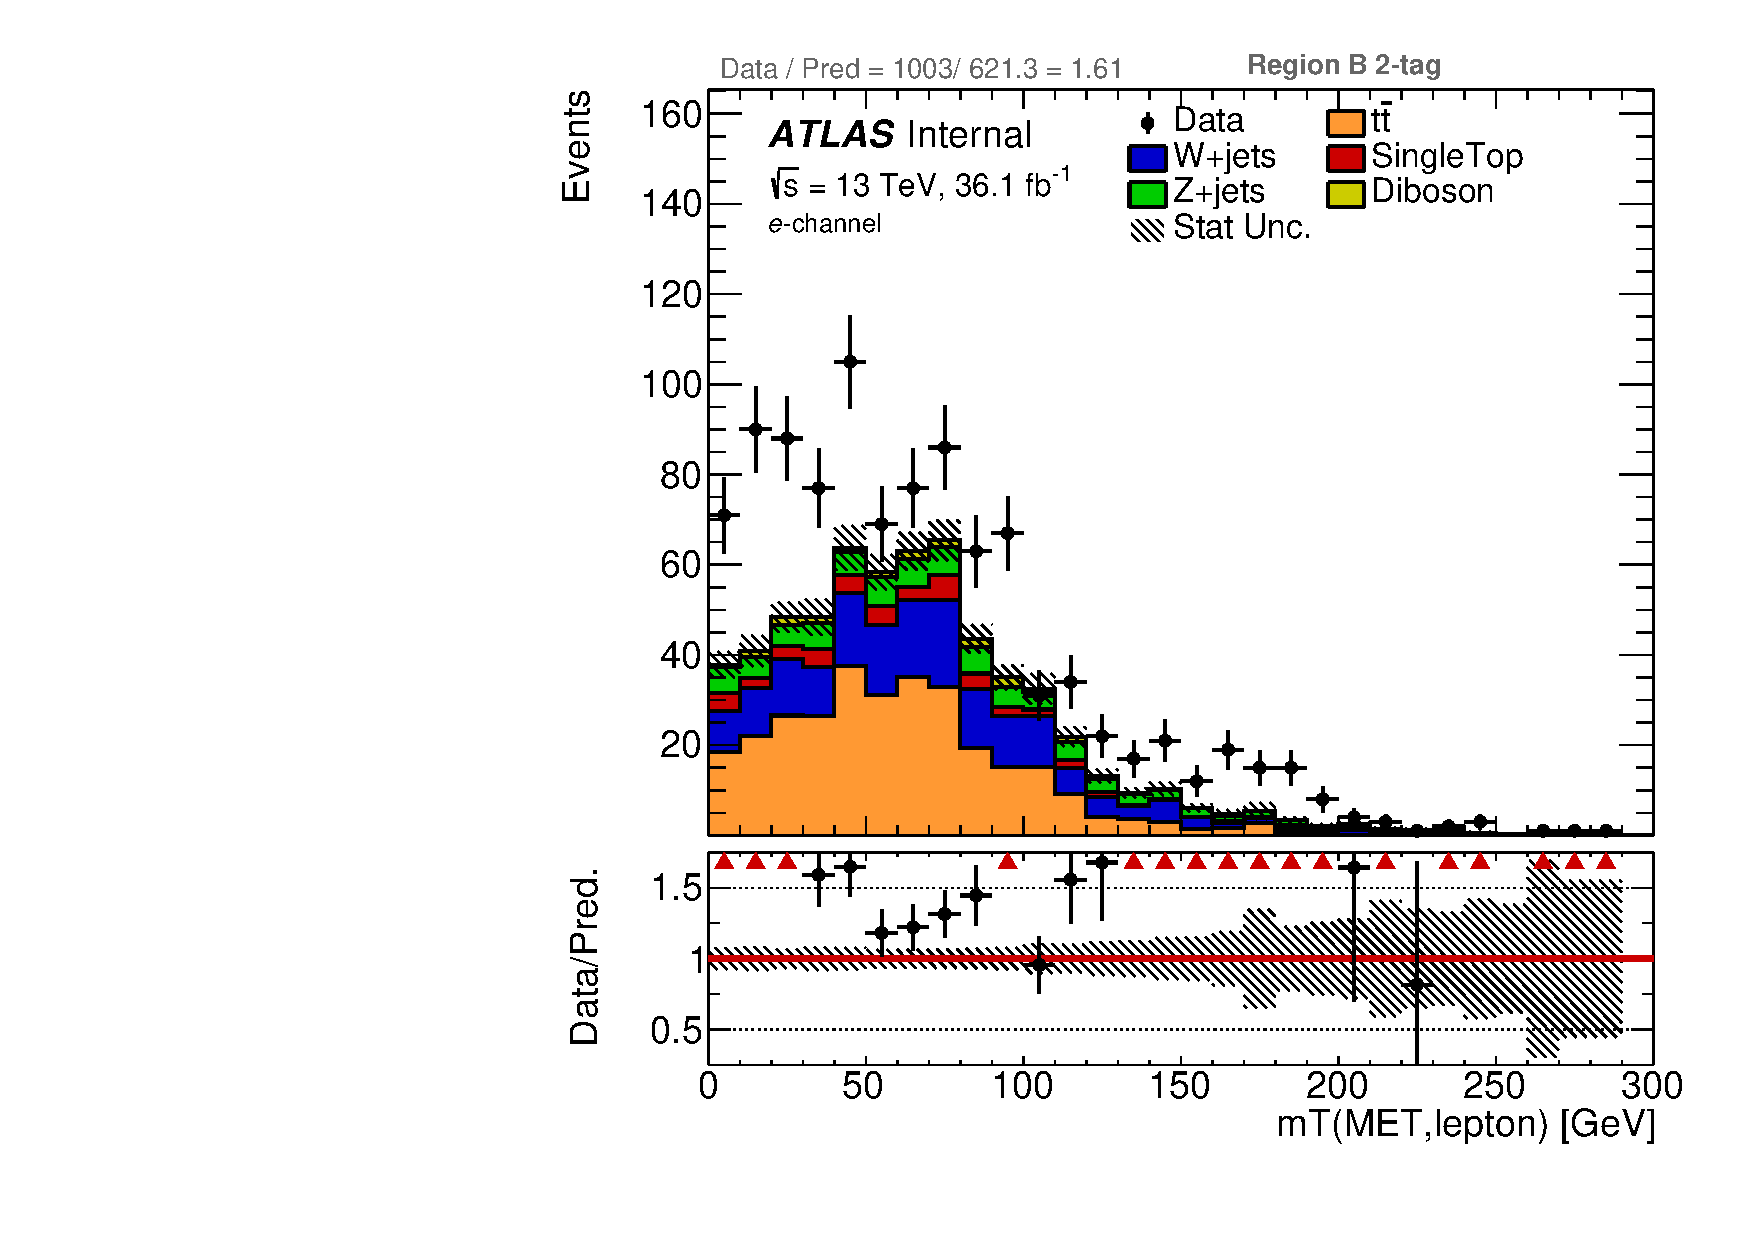
\includegraphics[scale=0.23]{./figures/boosted/ABCD/elec_Inc_RegionB_WlepMtATLAS}
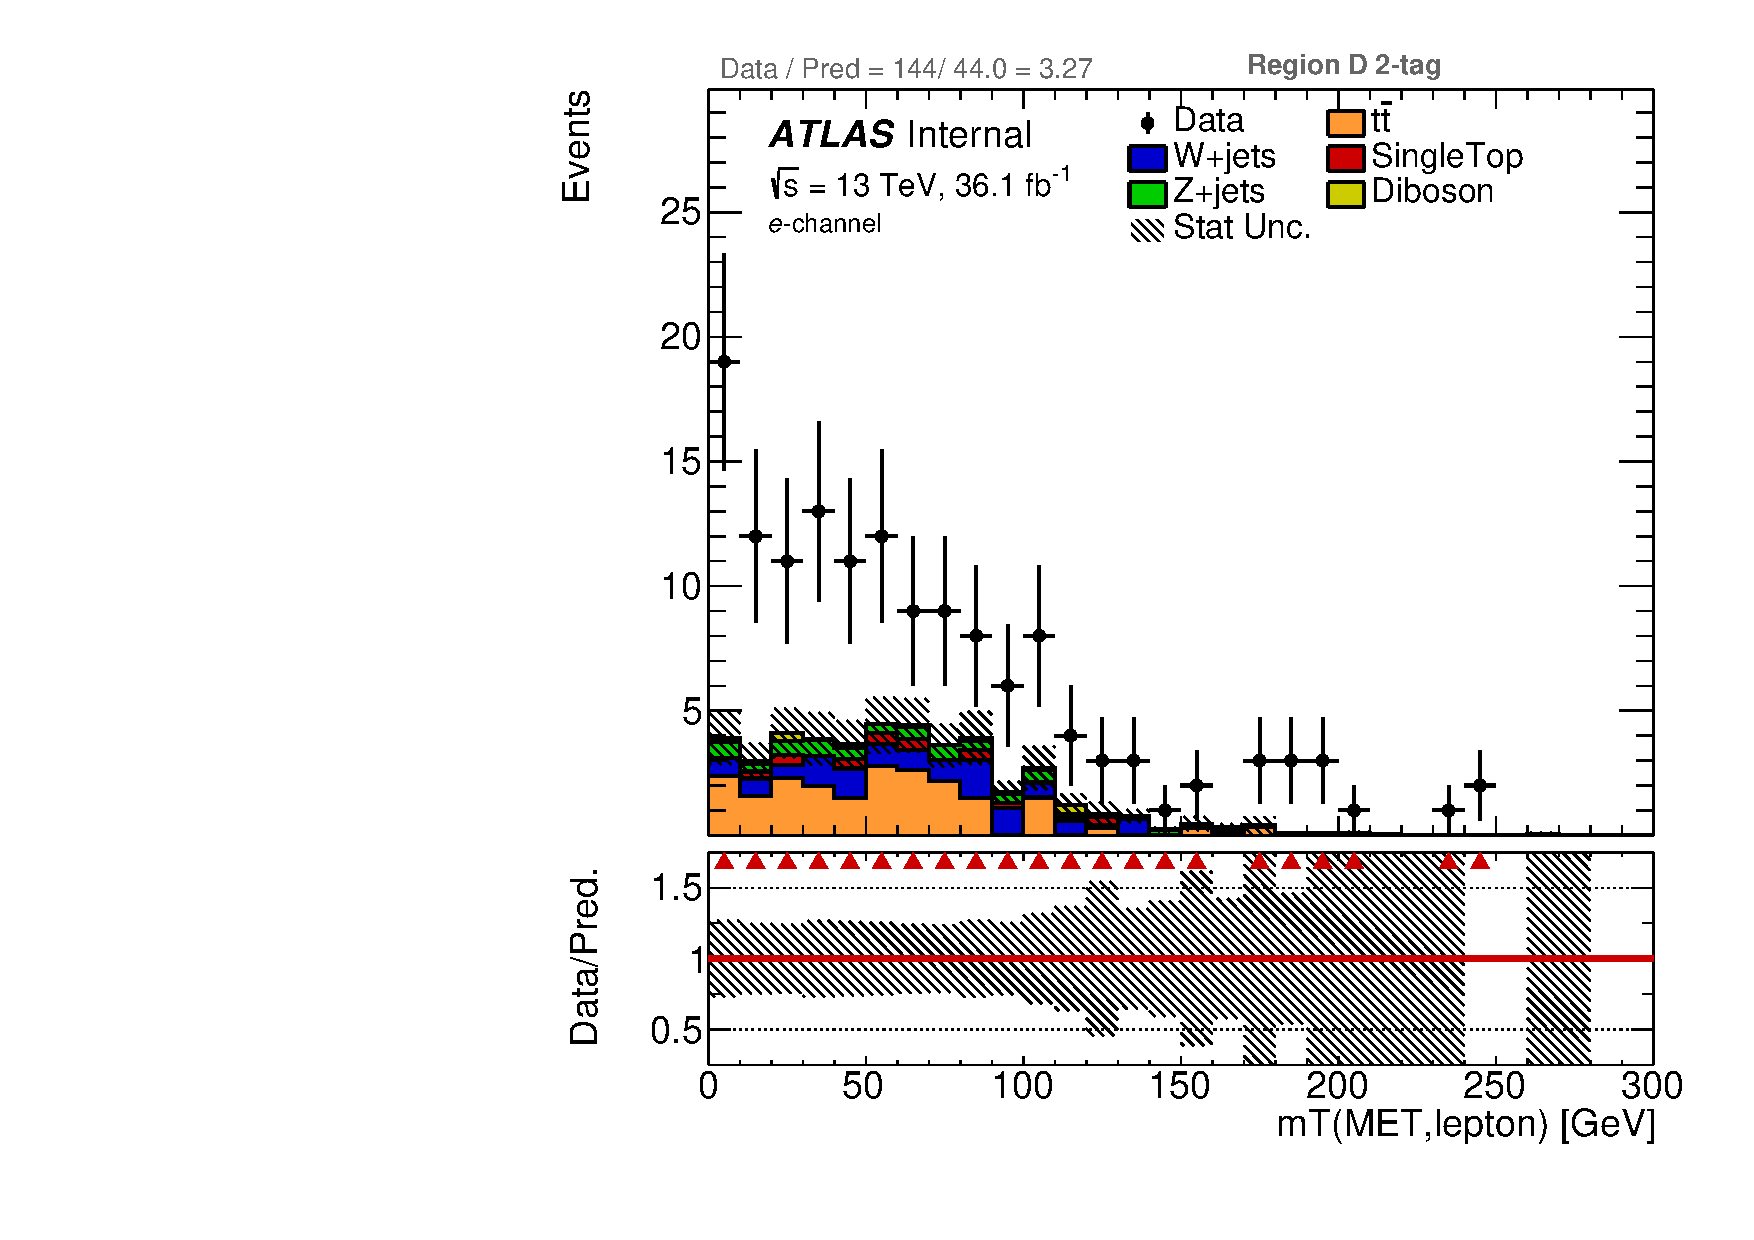
\includegraphics[scale=0.23]{./figures/boosted/ABCD/elec_Inc_RegionD_WlepMtATLAS}\\
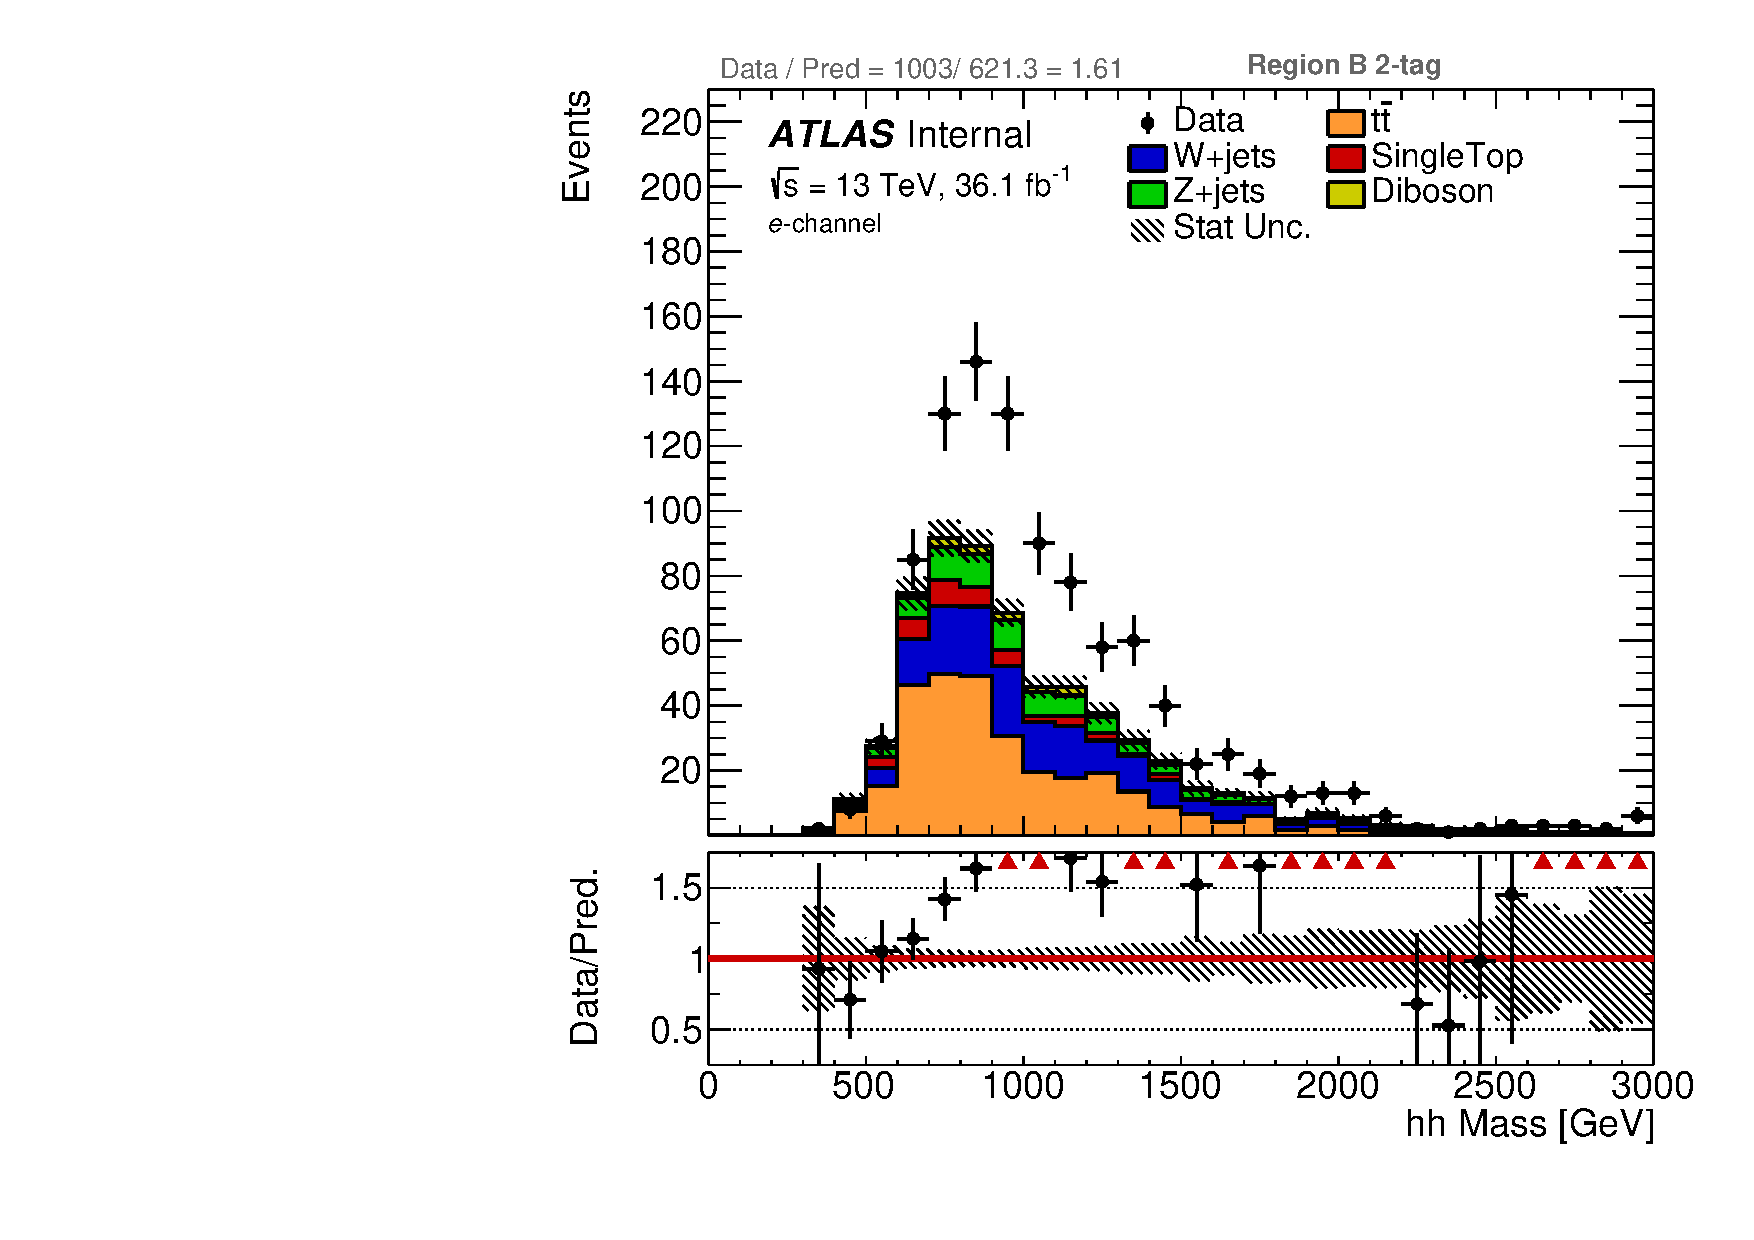
\includegraphics[scale=0.23]{./figures/boosted/ABCD/elec_Inc_RegionB_hhMass}
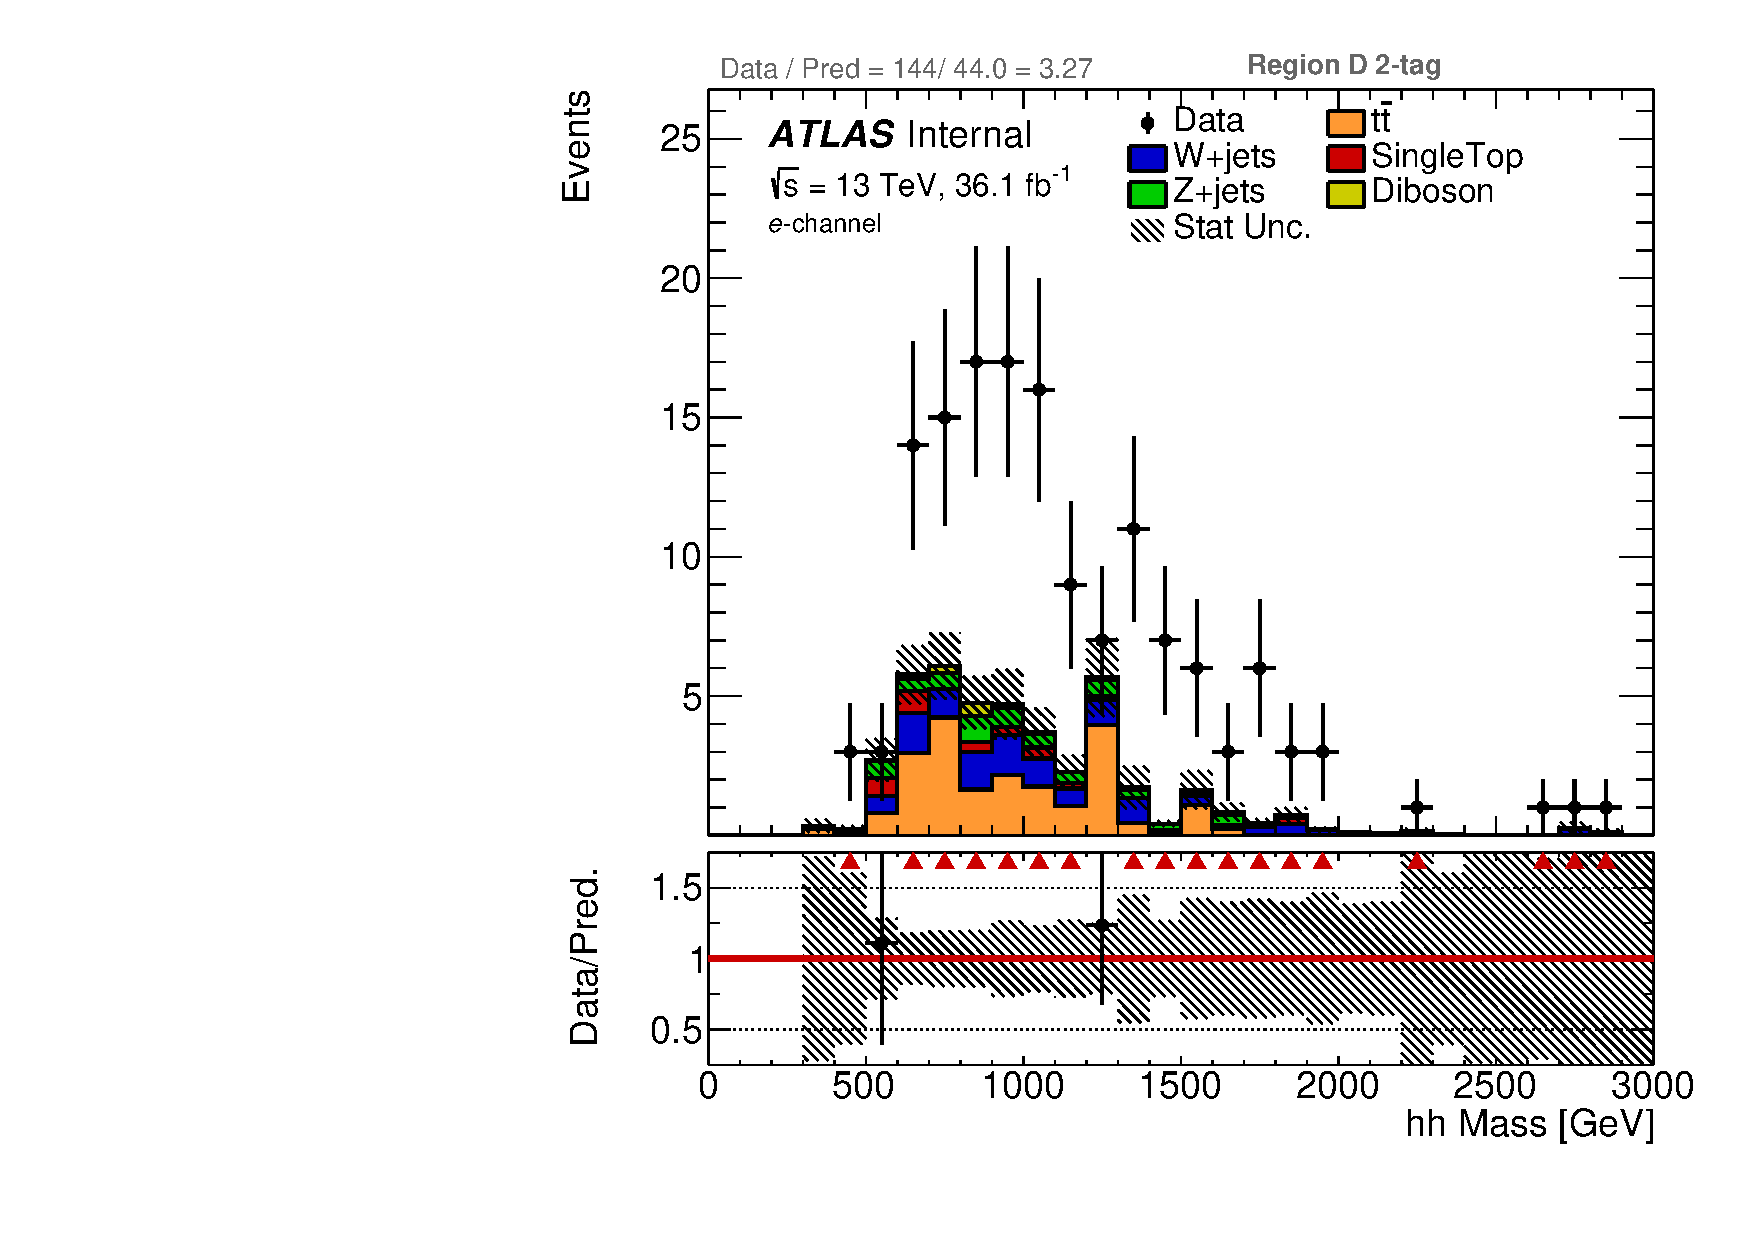
\includegraphics[scale=0.23]{./figures/boosted/ABCD/elec_Inc_RegionD_hhMass}
\caption{Kinematic distributions in ABCD method region B (left) and region D (right) in the electron channel.}
\label{fig:boosted_abcd_region_bd_elec}
\end{center}
\end{figure}

\begin{figure}[!htbp]
\begin{center}
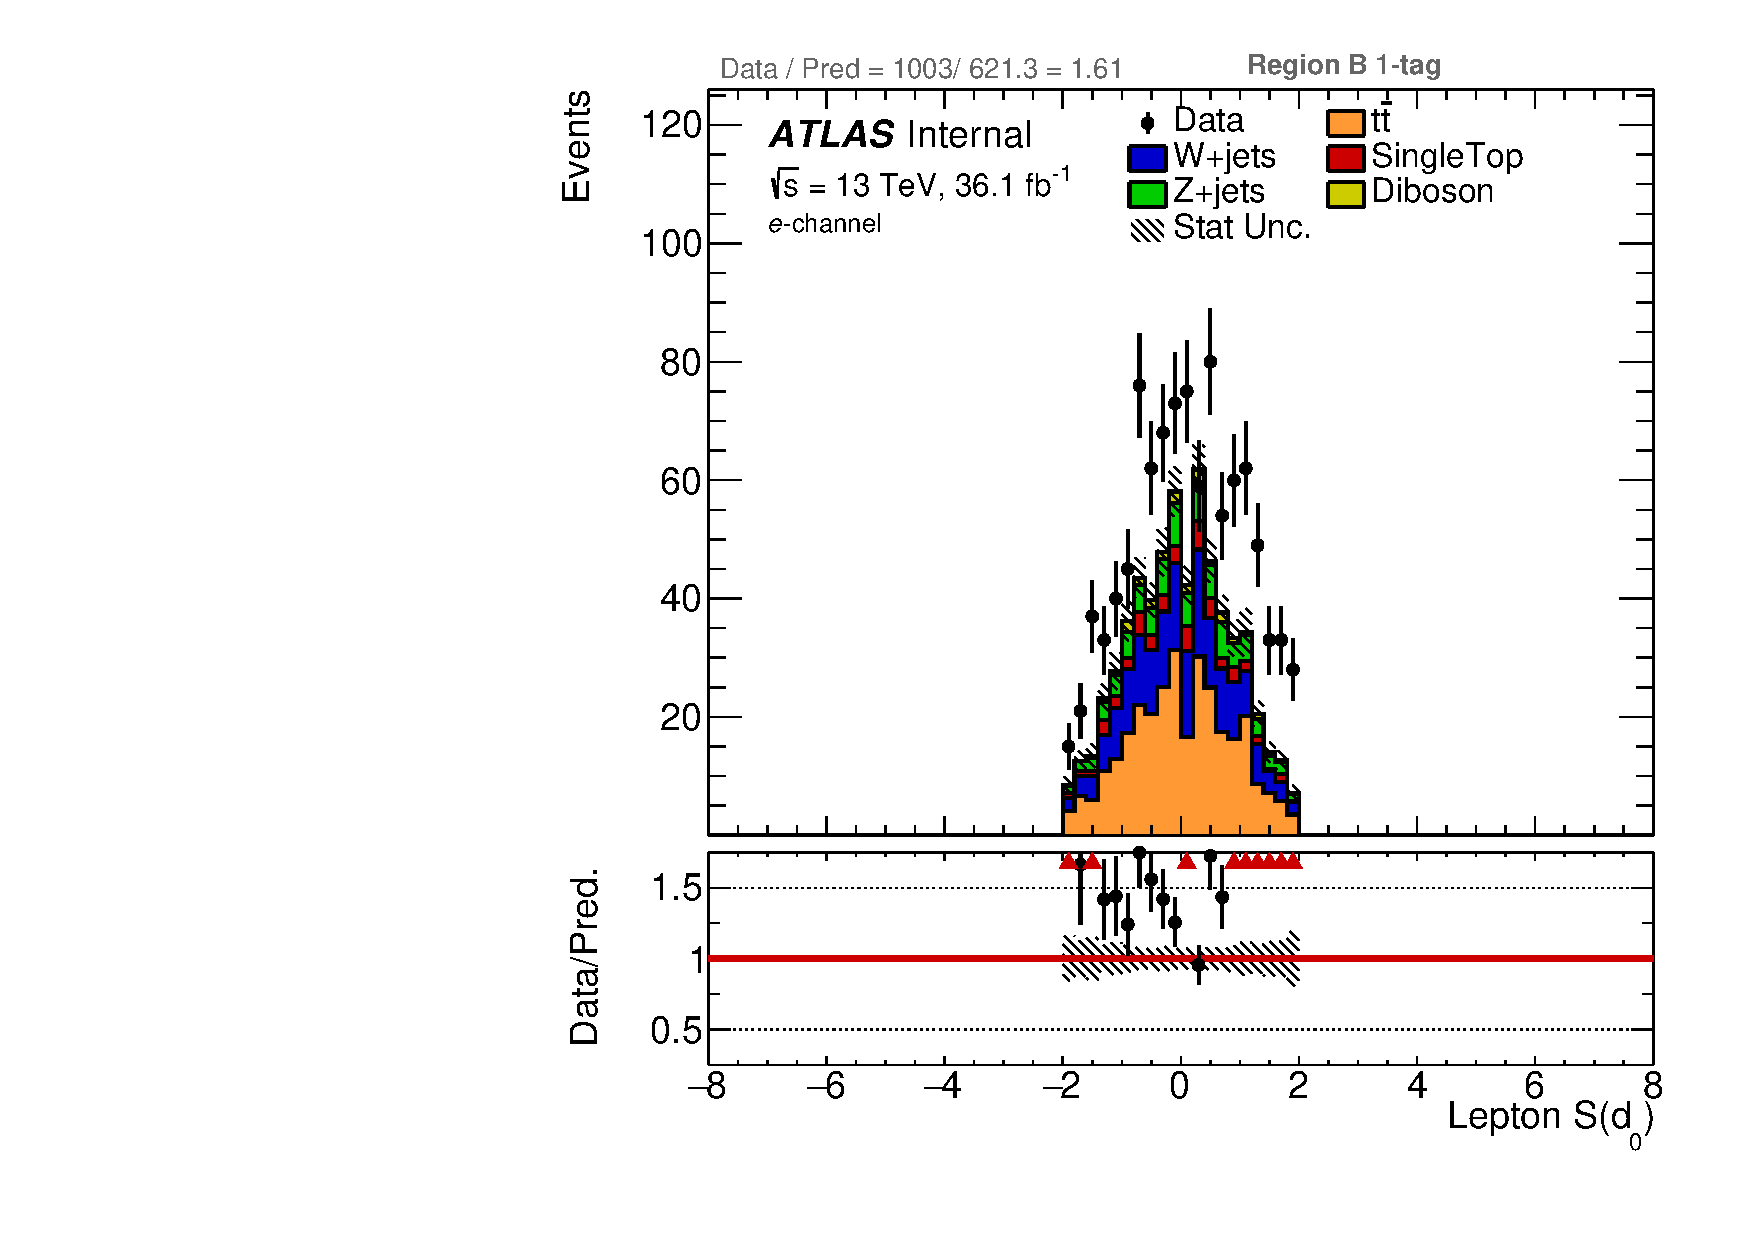
\includegraphics[scale=0.33]{./figures/boosted/ABCD/elec_Inc_RegionB_Lep_d0sigL}
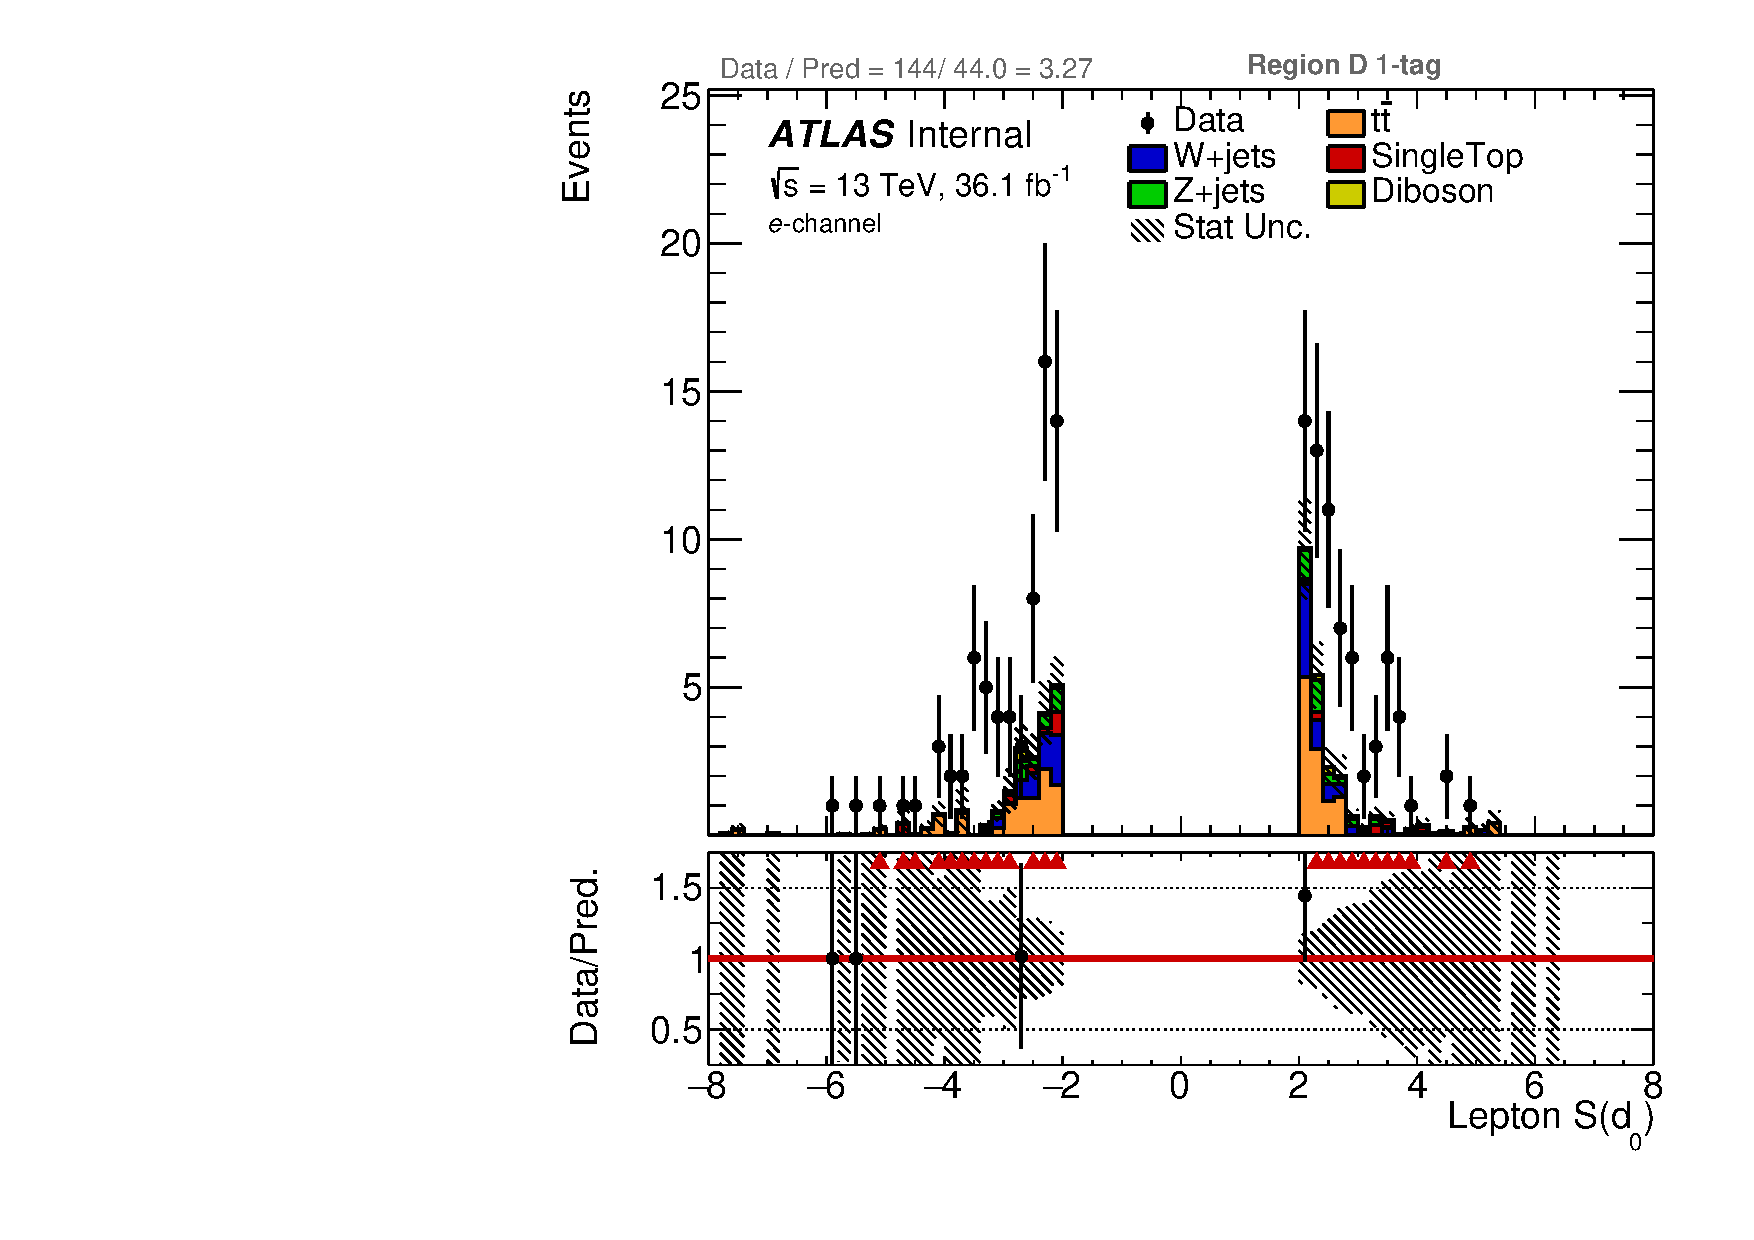
\includegraphics[scale=0.33]{./figures/boosted/ABCD/elec_Inc_RegionD_Lep_d0sigL}\\
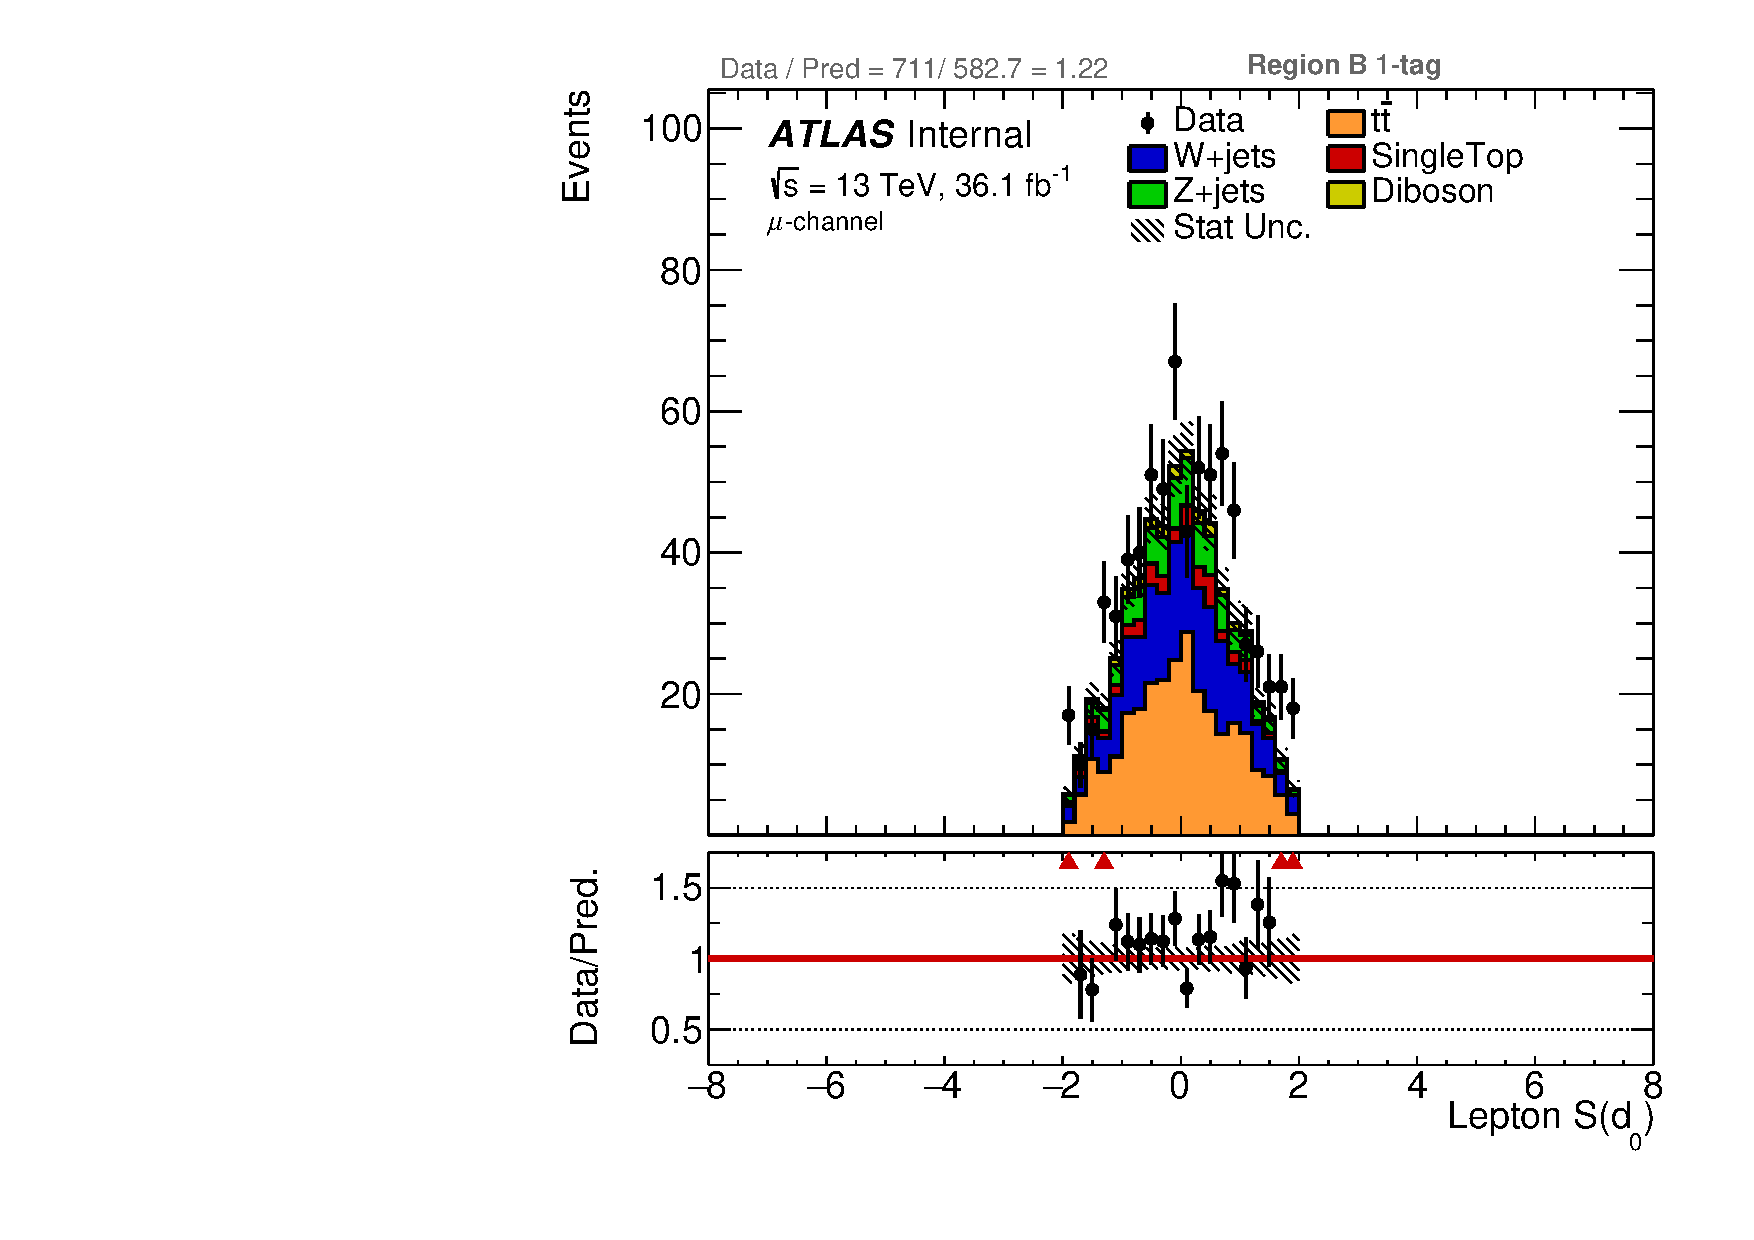
\includegraphics[scale=0.33]{./figures/boosted/ABCD/muon_Inc_RegionB_Lep_d0sigL}
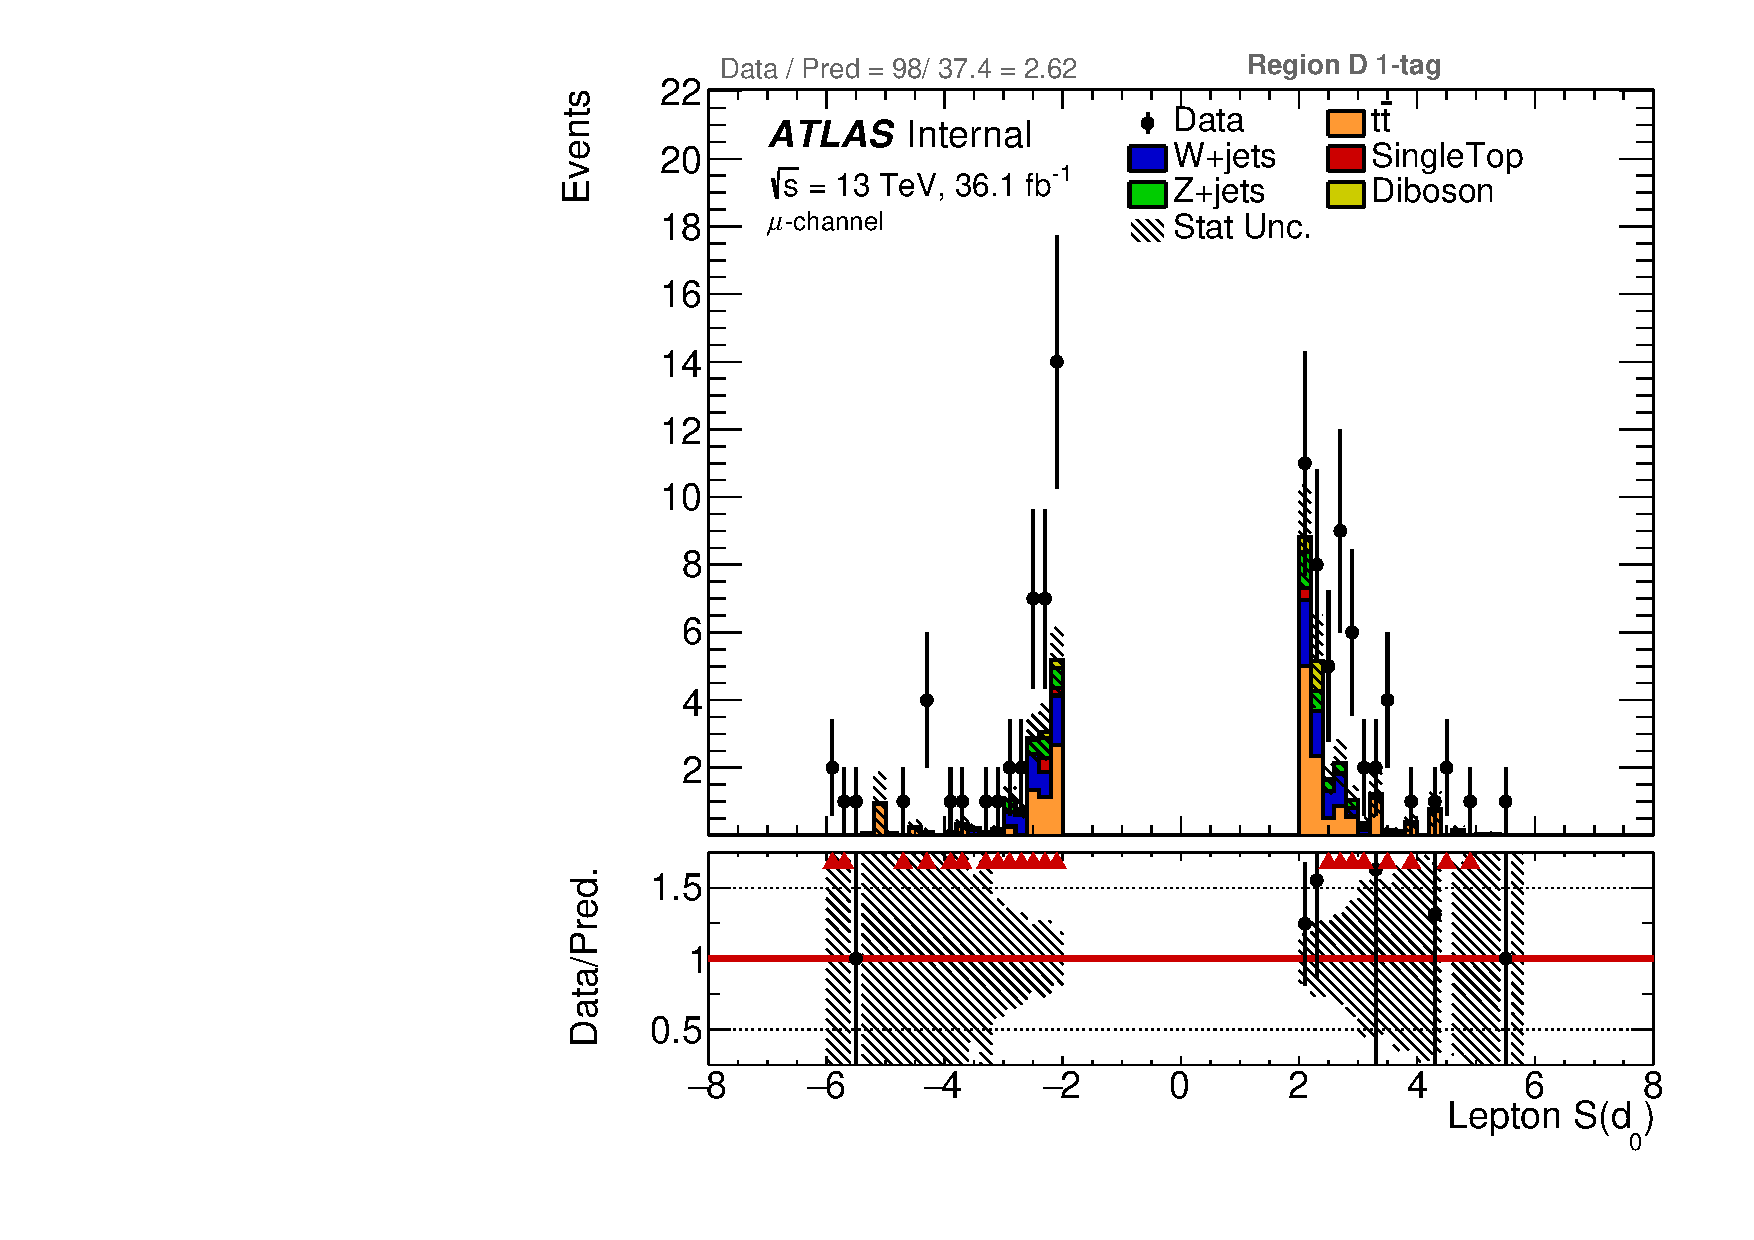
\includegraphics[scale=0.33]{./figures/boosted/ABCD/muon_Inc_RegionD_Lep_d0sigL}\\
\caption{$|d_{0}^{\textrm{sig}}|$ distributions in ABCD method region B (left) and region D (right) in the electron channel and muon channel.}
\label{fig:boosted_abcd_region_bd_d0sig}
\end{center}
\end{figure}

\FloatBarrier
%%%%%%%%%%%%%%%%%%%%%%%%
%
% Region C distributions
%
%%%%%%%%%%%%%%%%%%%%%%%
\subsection{Region C distributions}
\label{app:boosted_qcd_region_c}

Figure~\ref{fig:boosted_abcd_region_c_mbbcr_muon} and~\ref{fig:boosted_abcd_region_c_mbbcr_elec} show several kinematic distributions
region C mBB control region for the muon channel and electron channel respectively. Figure~\ref{fig:boosted_abcd_region_c_SR_muon}
and~\ref{fig:boosted_abcd_region_c_SR_elec} show several kinematic distributions region C signal region for the muon channel and 
electron channel respectively.

\begin{figure}[!htbp]
\begin{center}
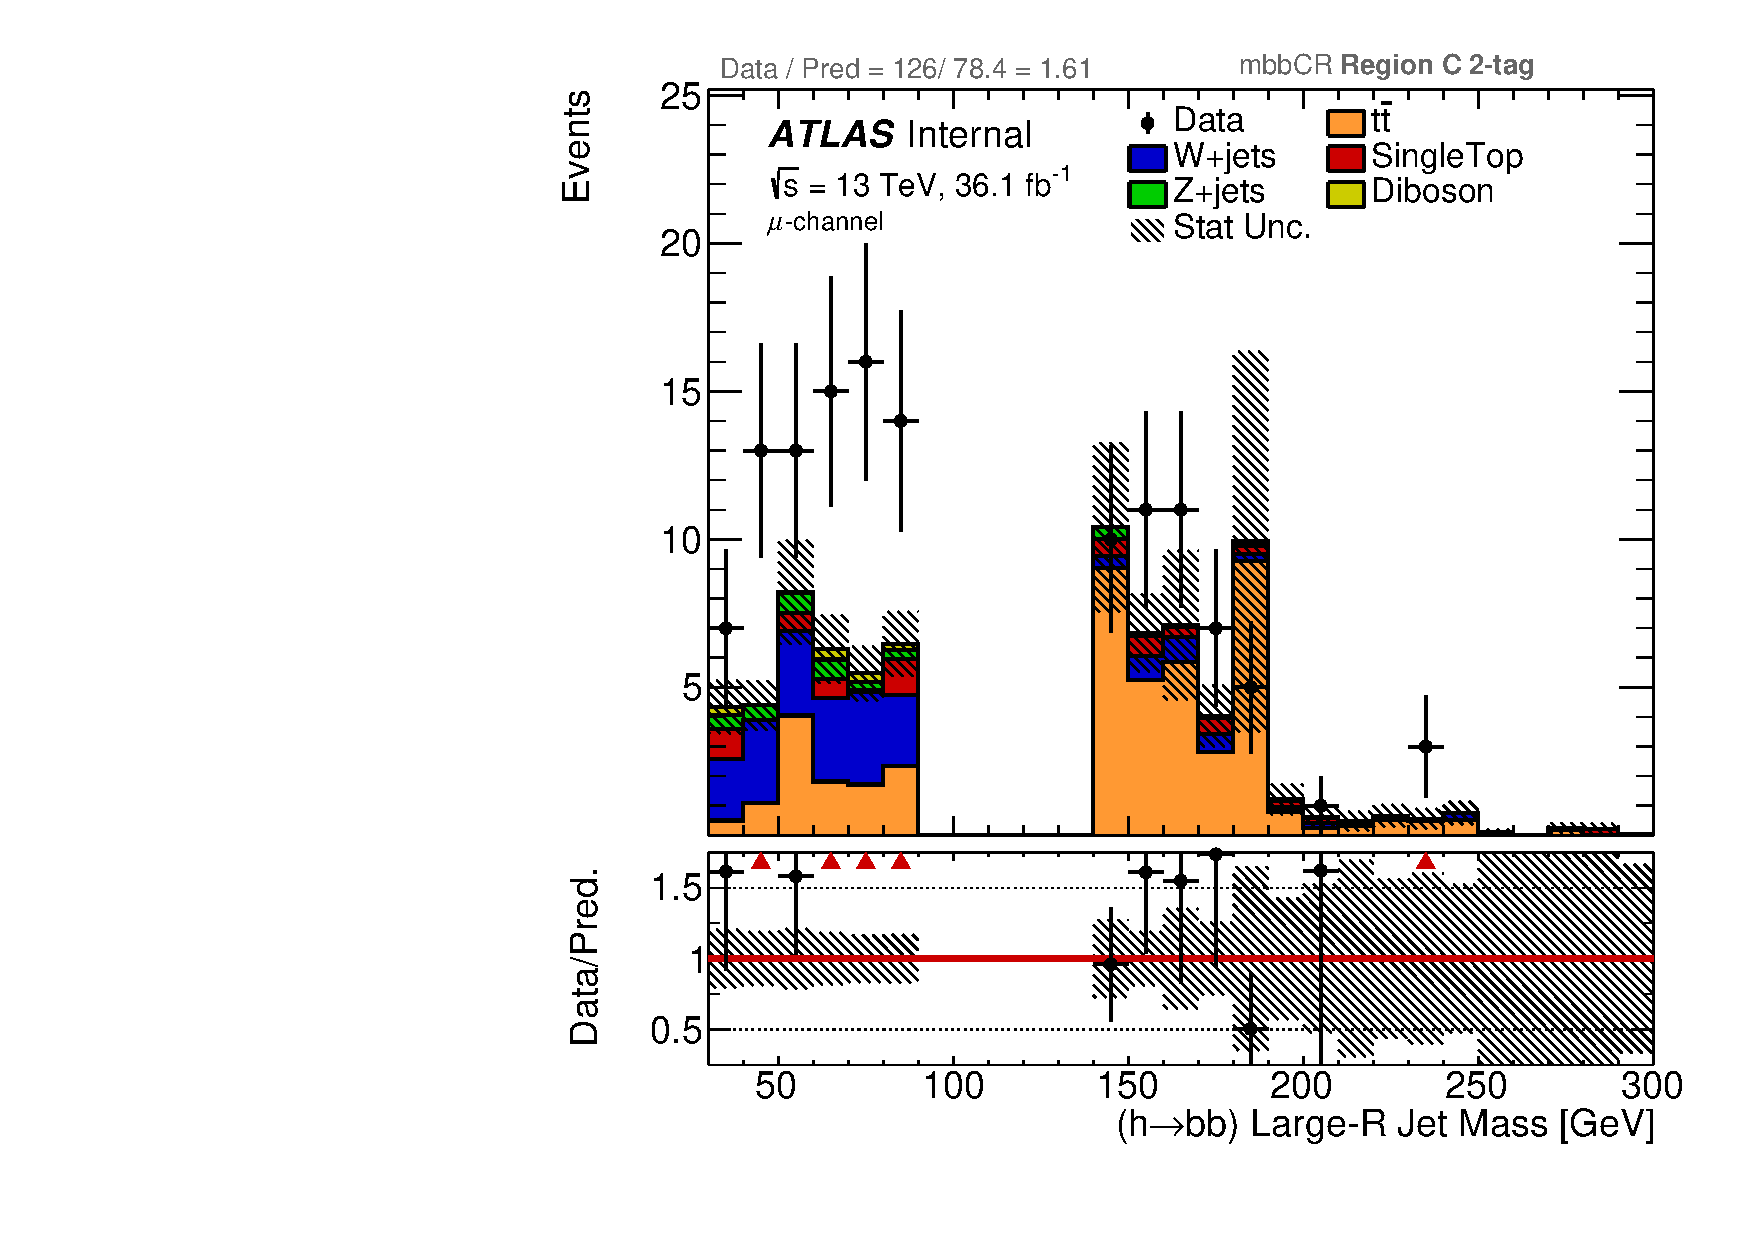
\includegraphics[scale=0.23]{./figures/boosted/ABCD/muon_mbbcr_RegionC_HbbMass}
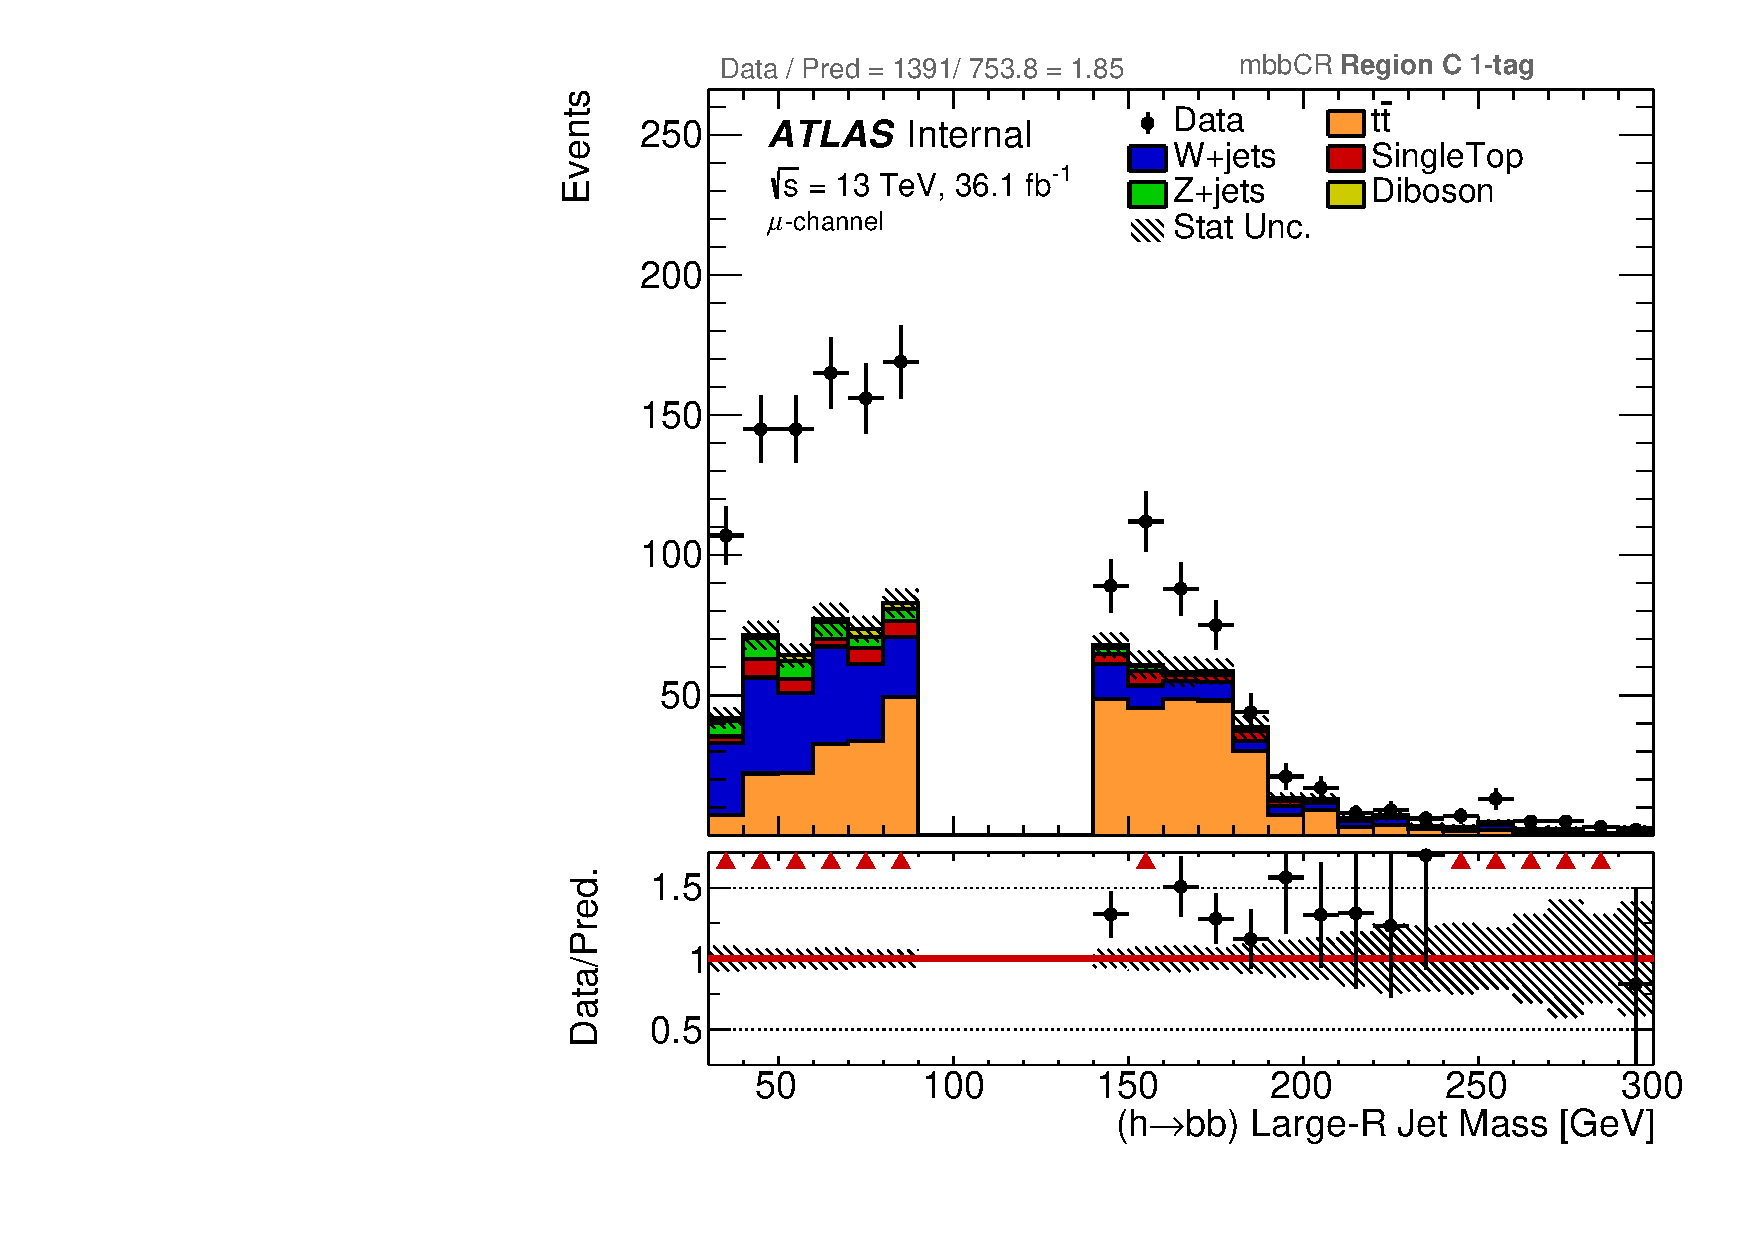
\includegraphics[scale=0.23]{./figures/boosted/ABCD/muon_mbbcr_RegionC_1tag_HbbMass}\\
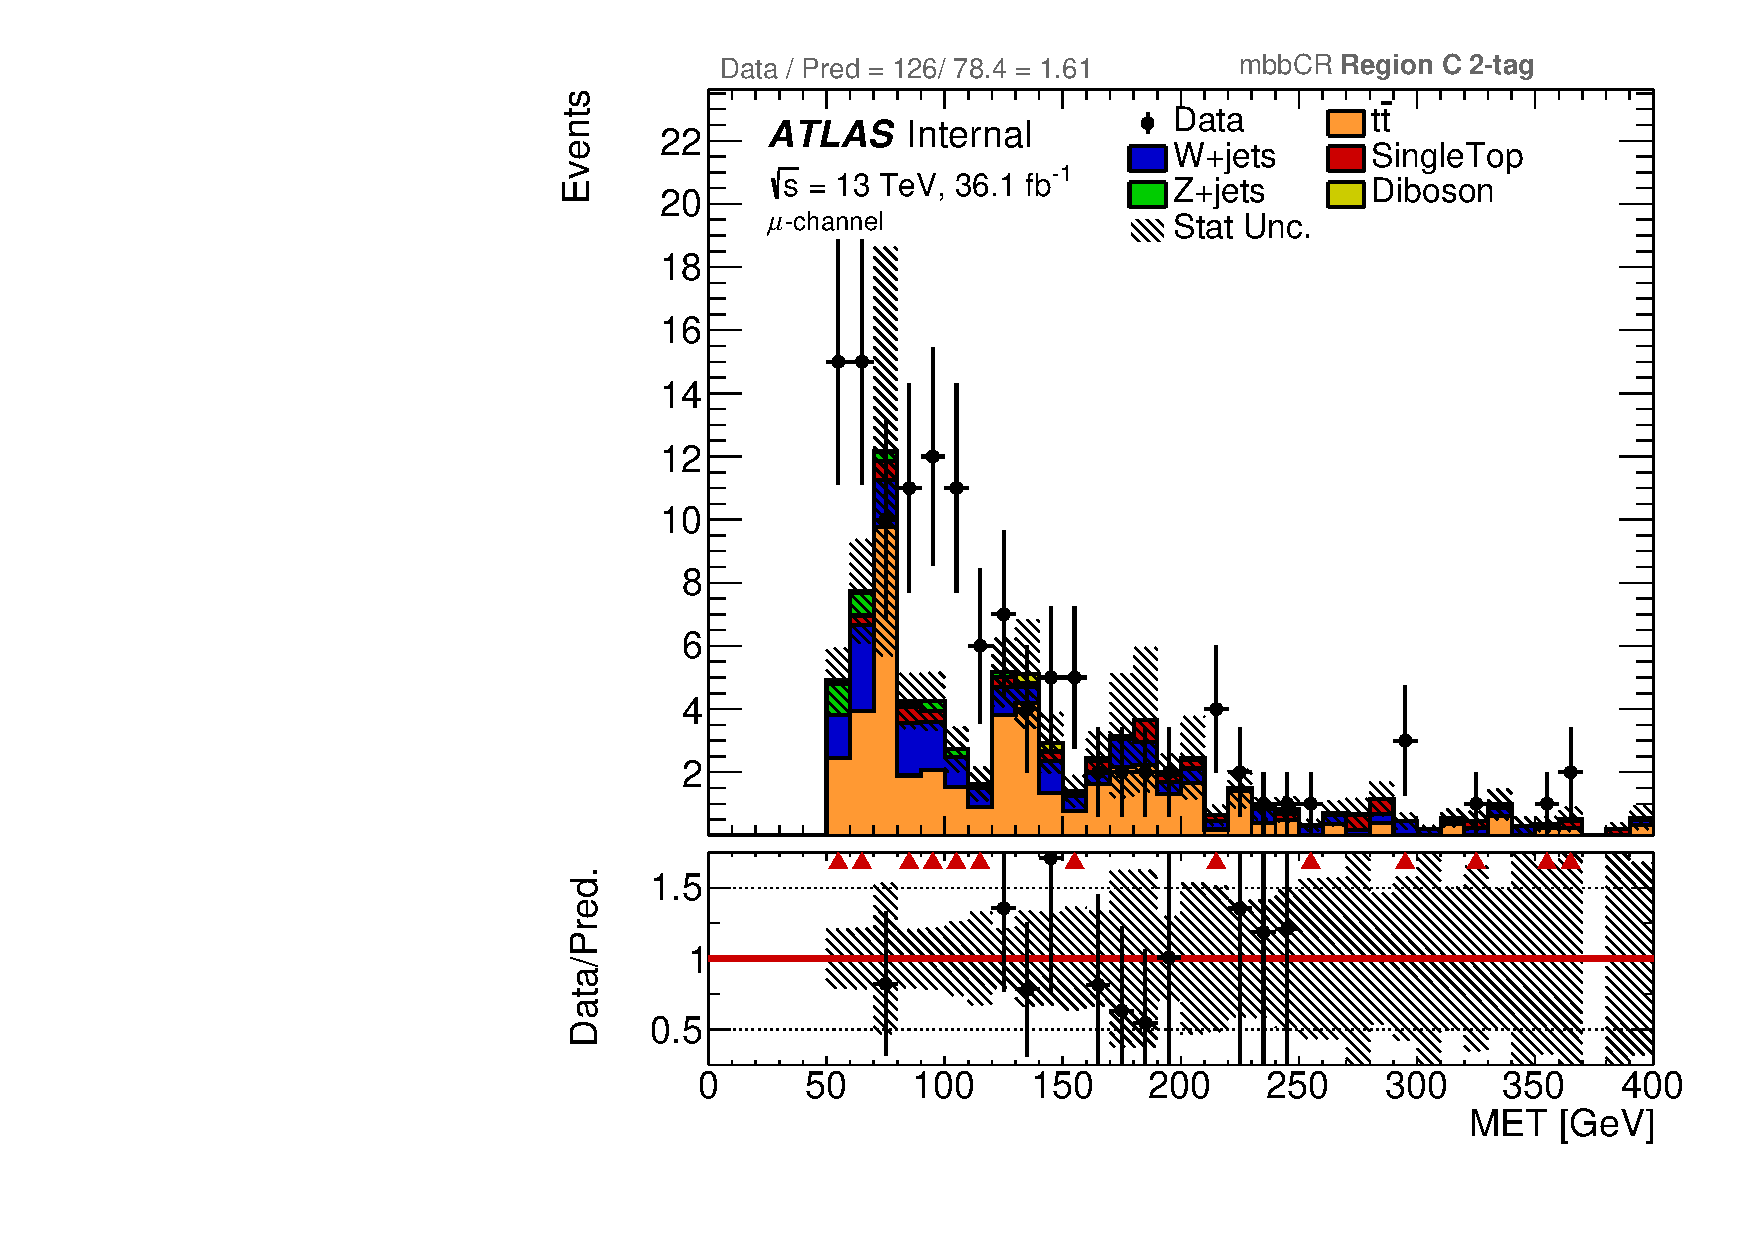
\includegraphics[scale=0.23]{./figures/boosted/ABCD/muon_mbbcr_RegionC_MET}
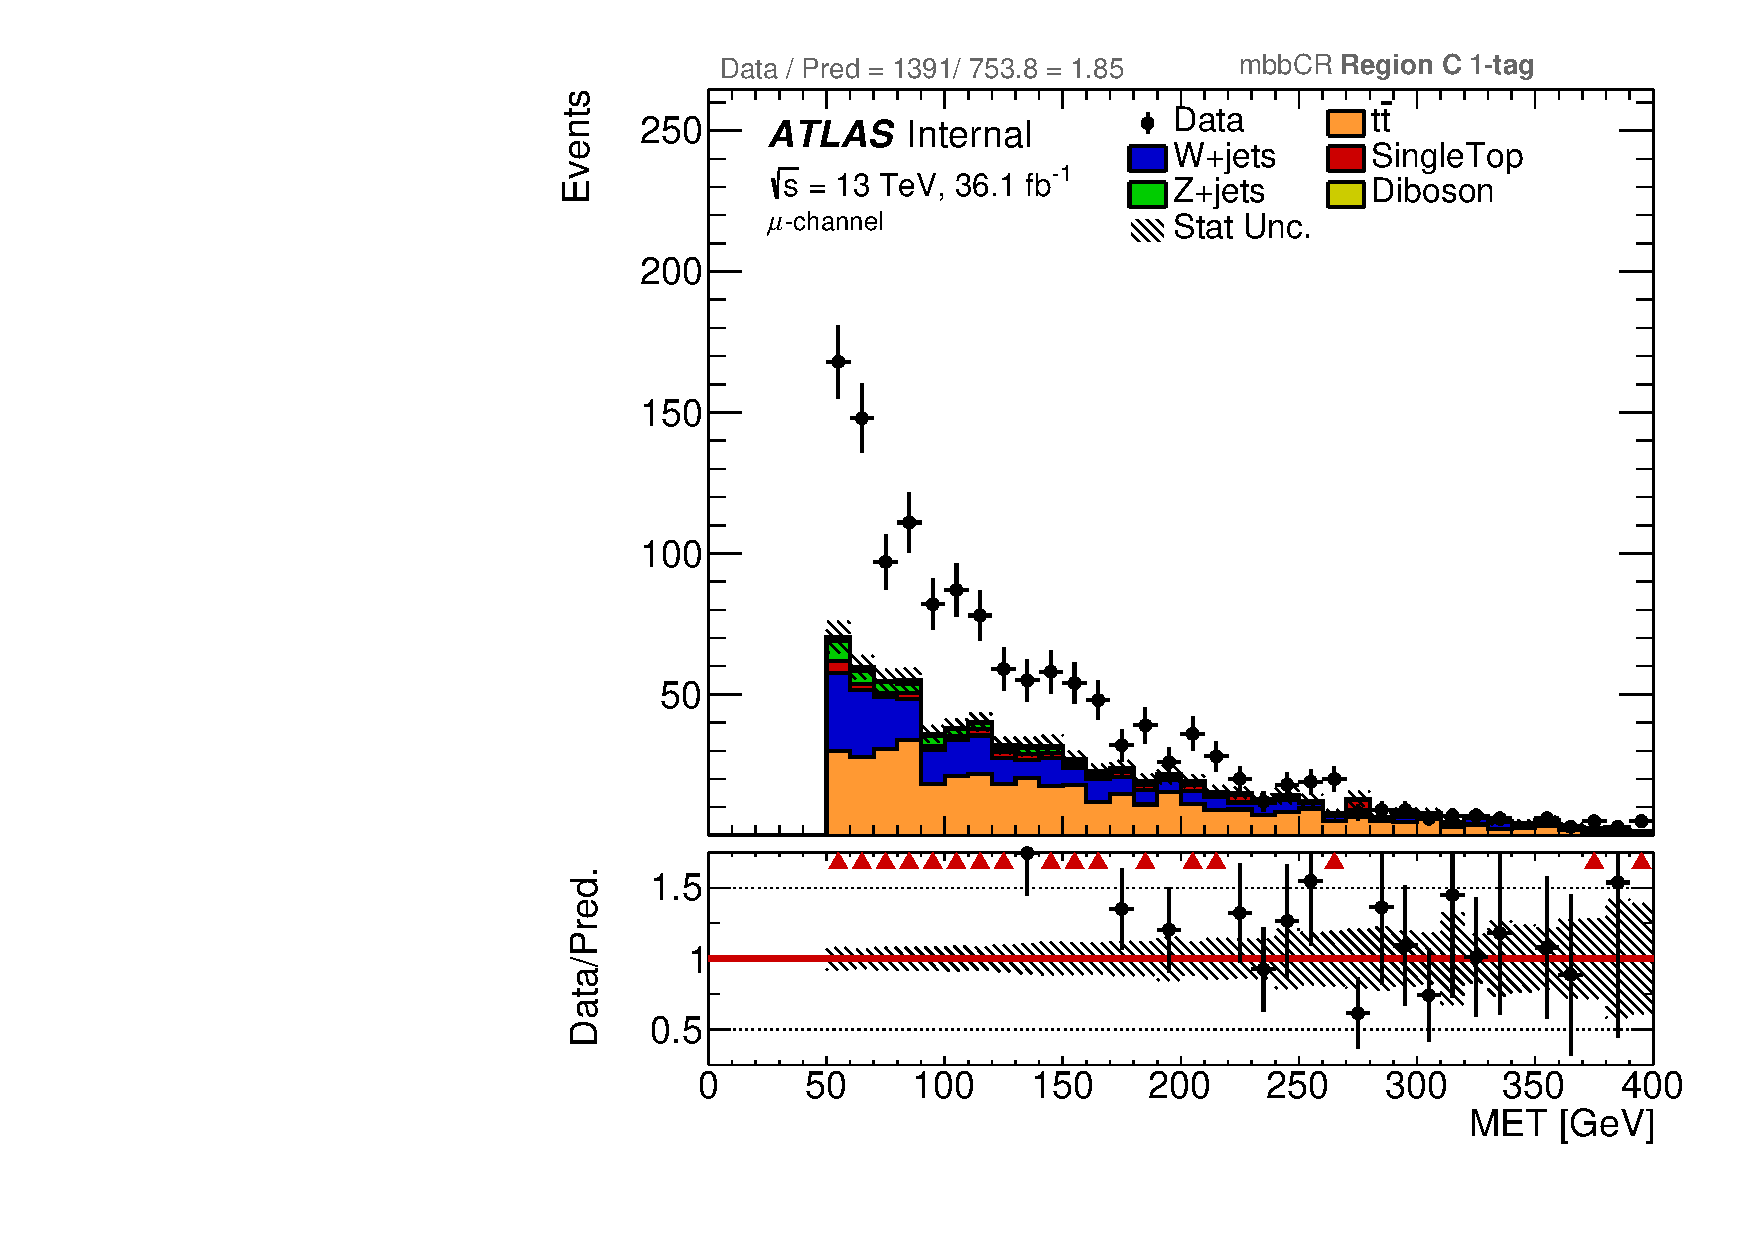
\includegraphics[scale=0.23]{./figures/boosted/ABCD/muon_mbbcr_RegionC_1tag_MET}\\
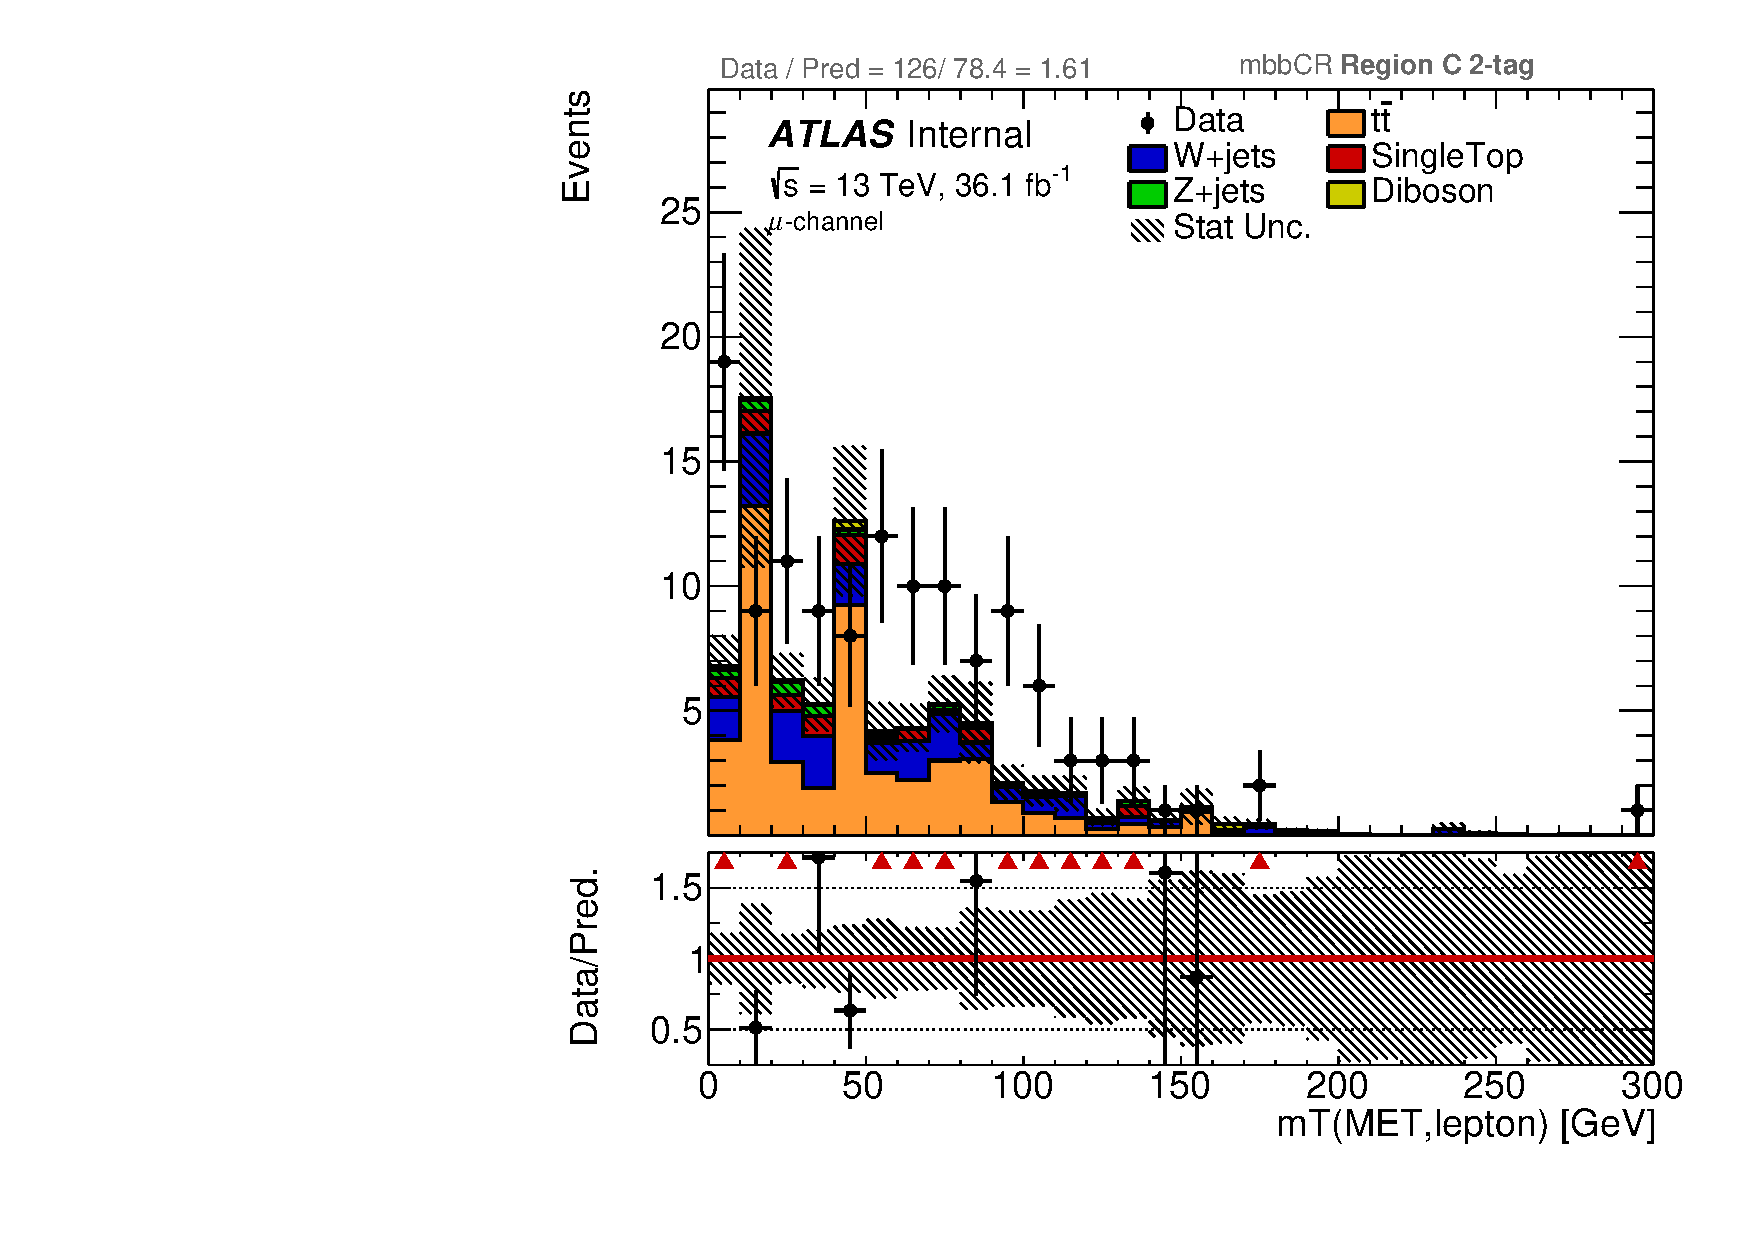
\includegraphics[scale=0.23]{./figures/boosted/ABCD/muon_mbbcr_RegionC_WlepMtATLAS}
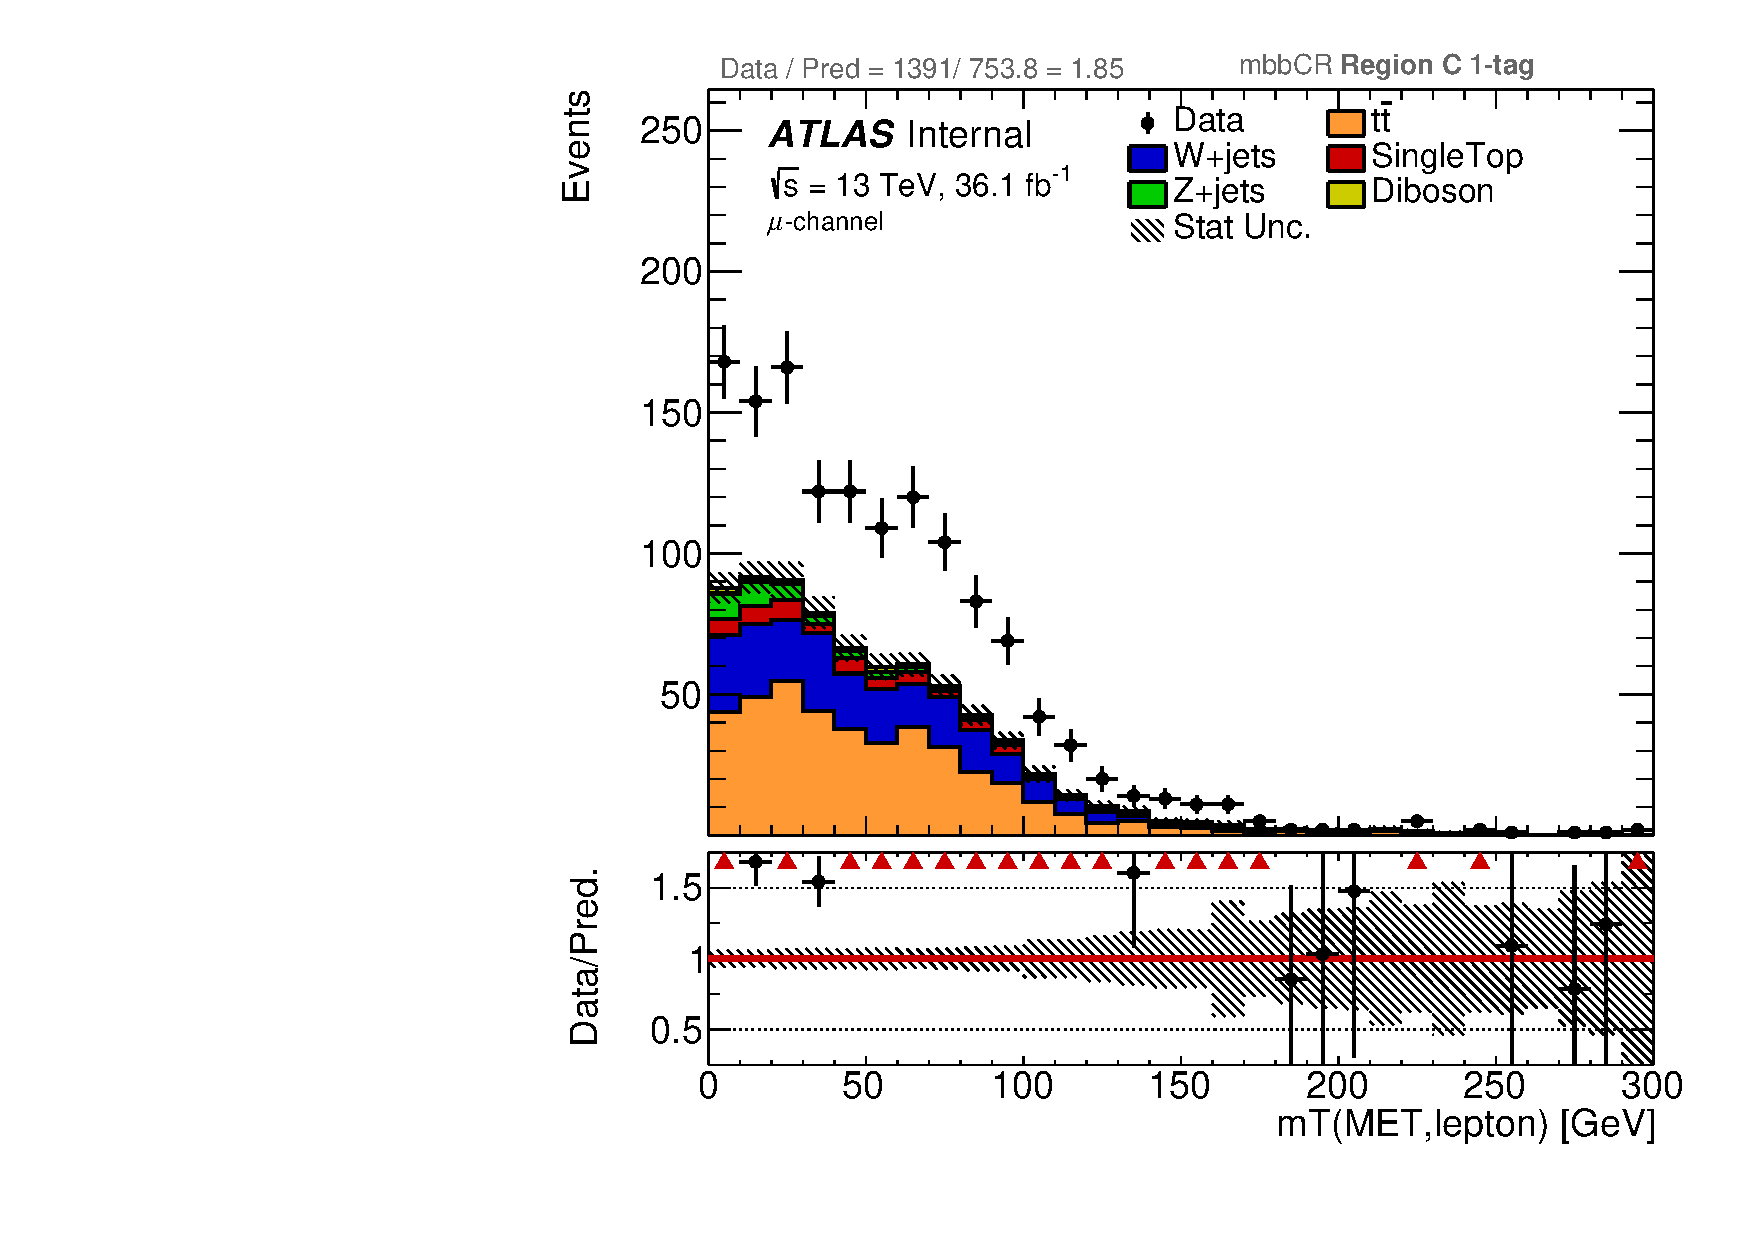
\includegraphics[scale=0.23]{./figures/boosted/ABCD/muon_mbbcr_RegionC_1tag_WlepMtATLAS}\\
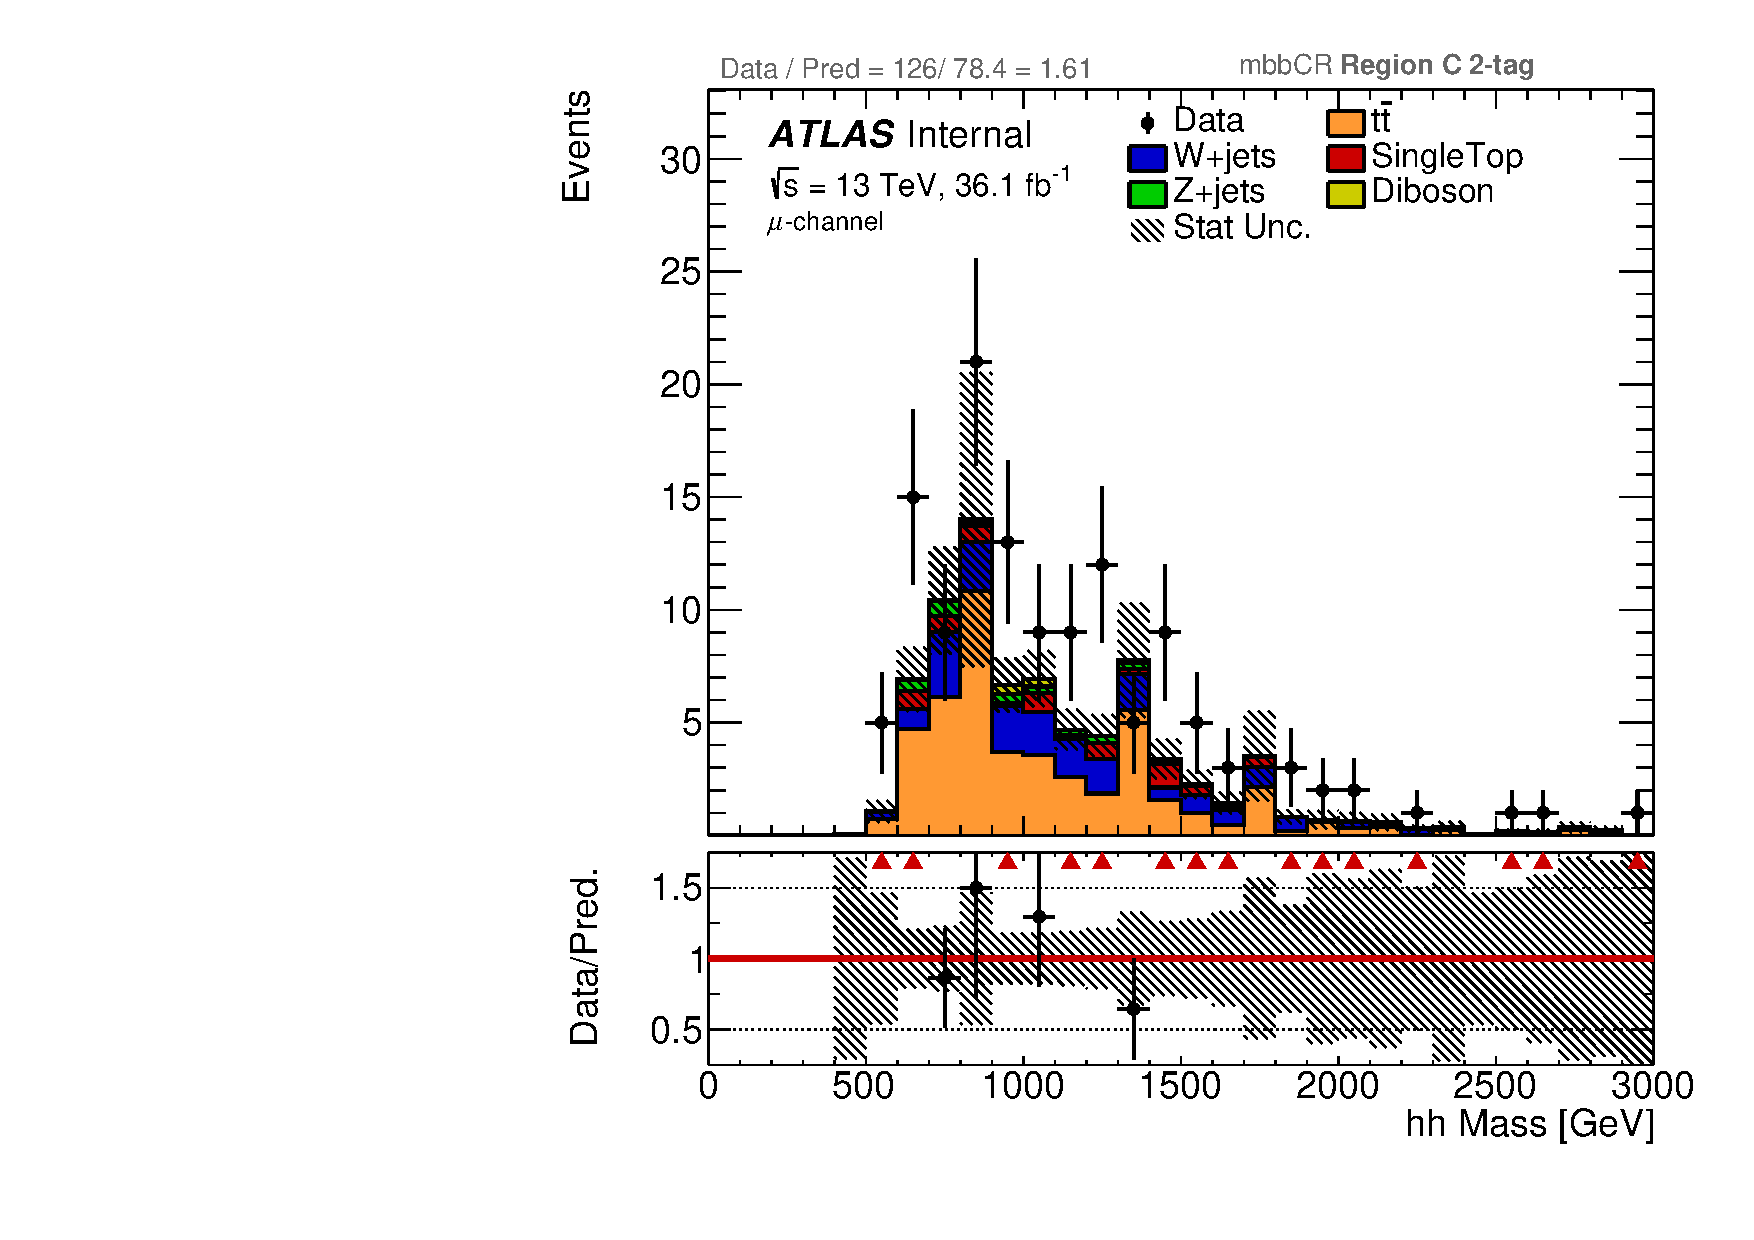
\includegraphics[scale=0.23]{./figures/boosted/ABCD/muon_mbbcr_RegionC_hhMass}
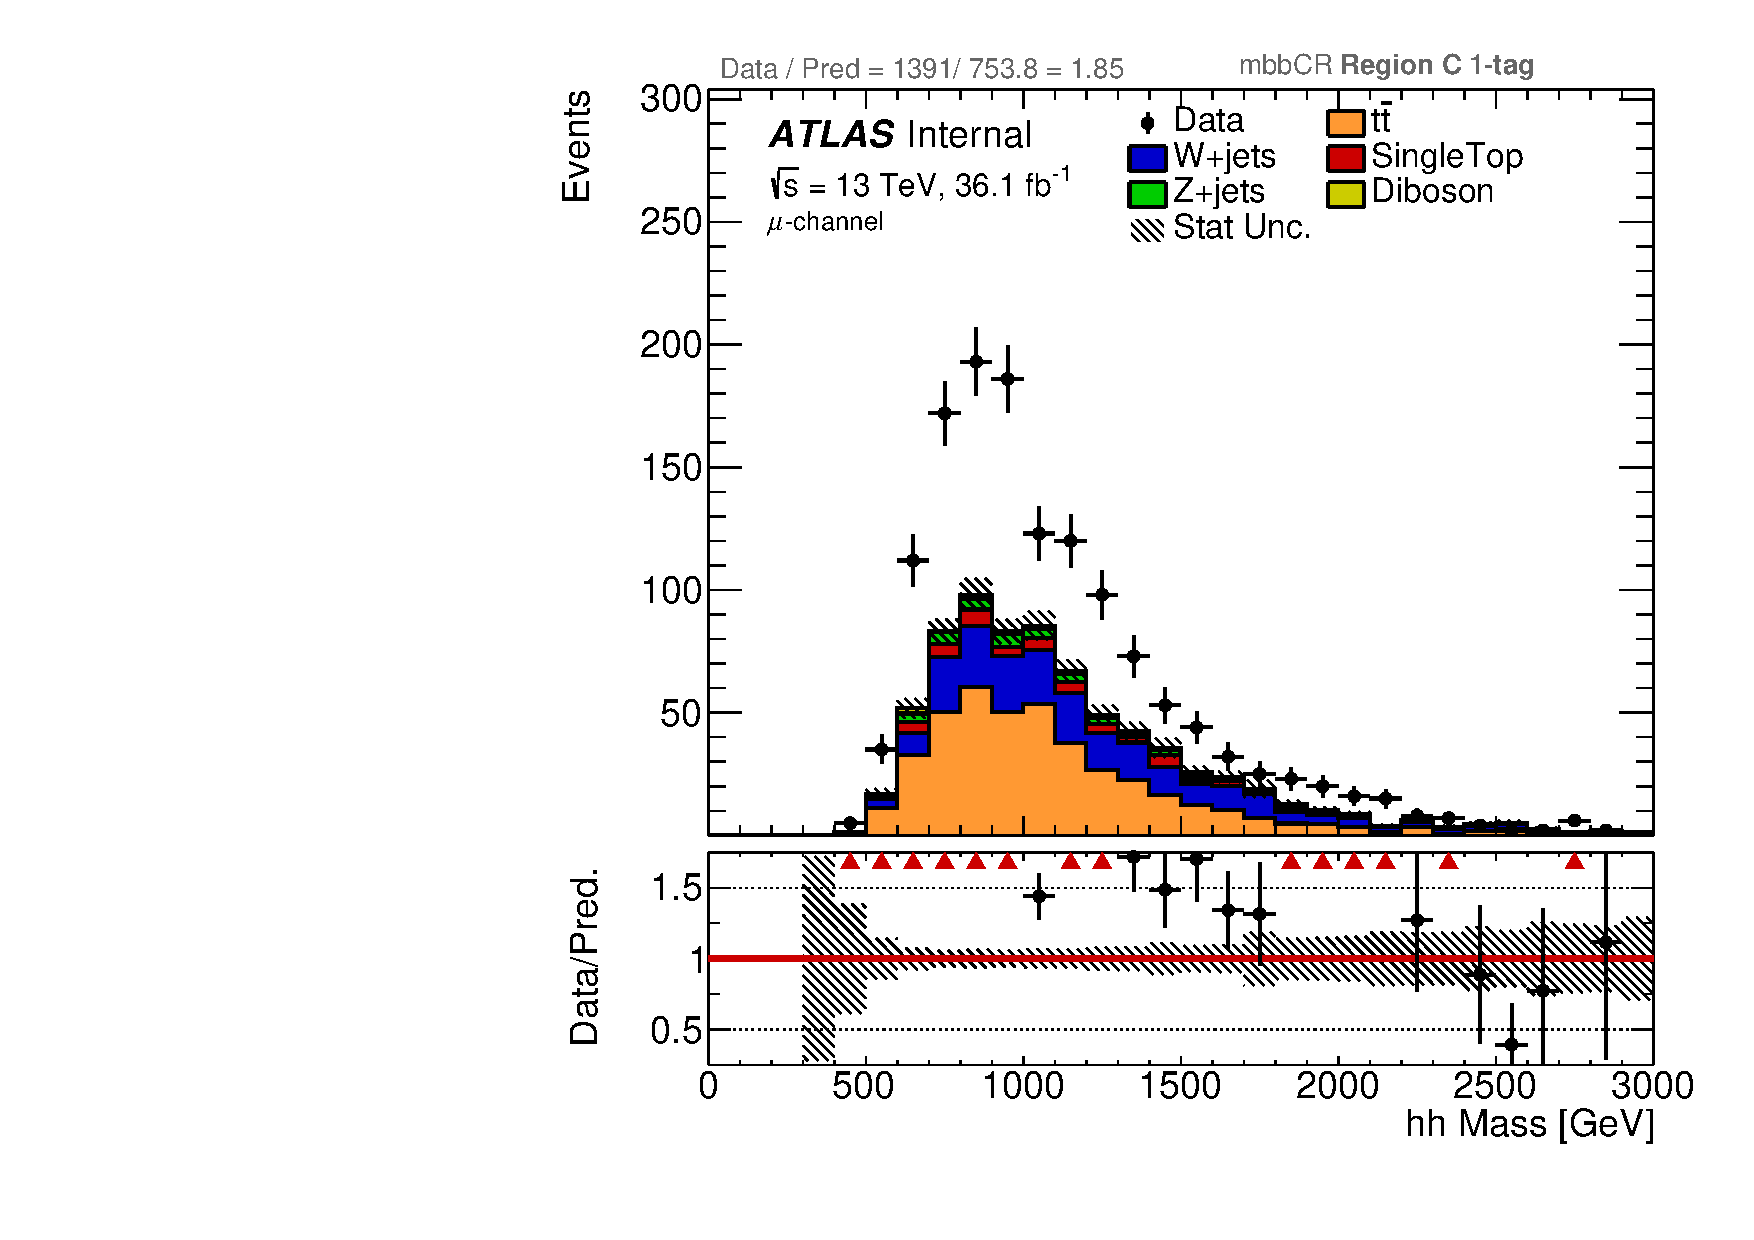
\includegraphics[scale=0.23]{./figures/boosted/ABCD/muon_mbbcr_RegionC_1tag_hhMass}
\caption{Kinematic distributions in ABCD method region C of 2-tag events (left) and 1-tag events (right) in the muon channel mBBcr.}
\label{fig:boosted_abcd_region_c_mbbcr_muon}
\end{center}
\end{figure}

\begin{figure}[!htbp]
\begin{center}
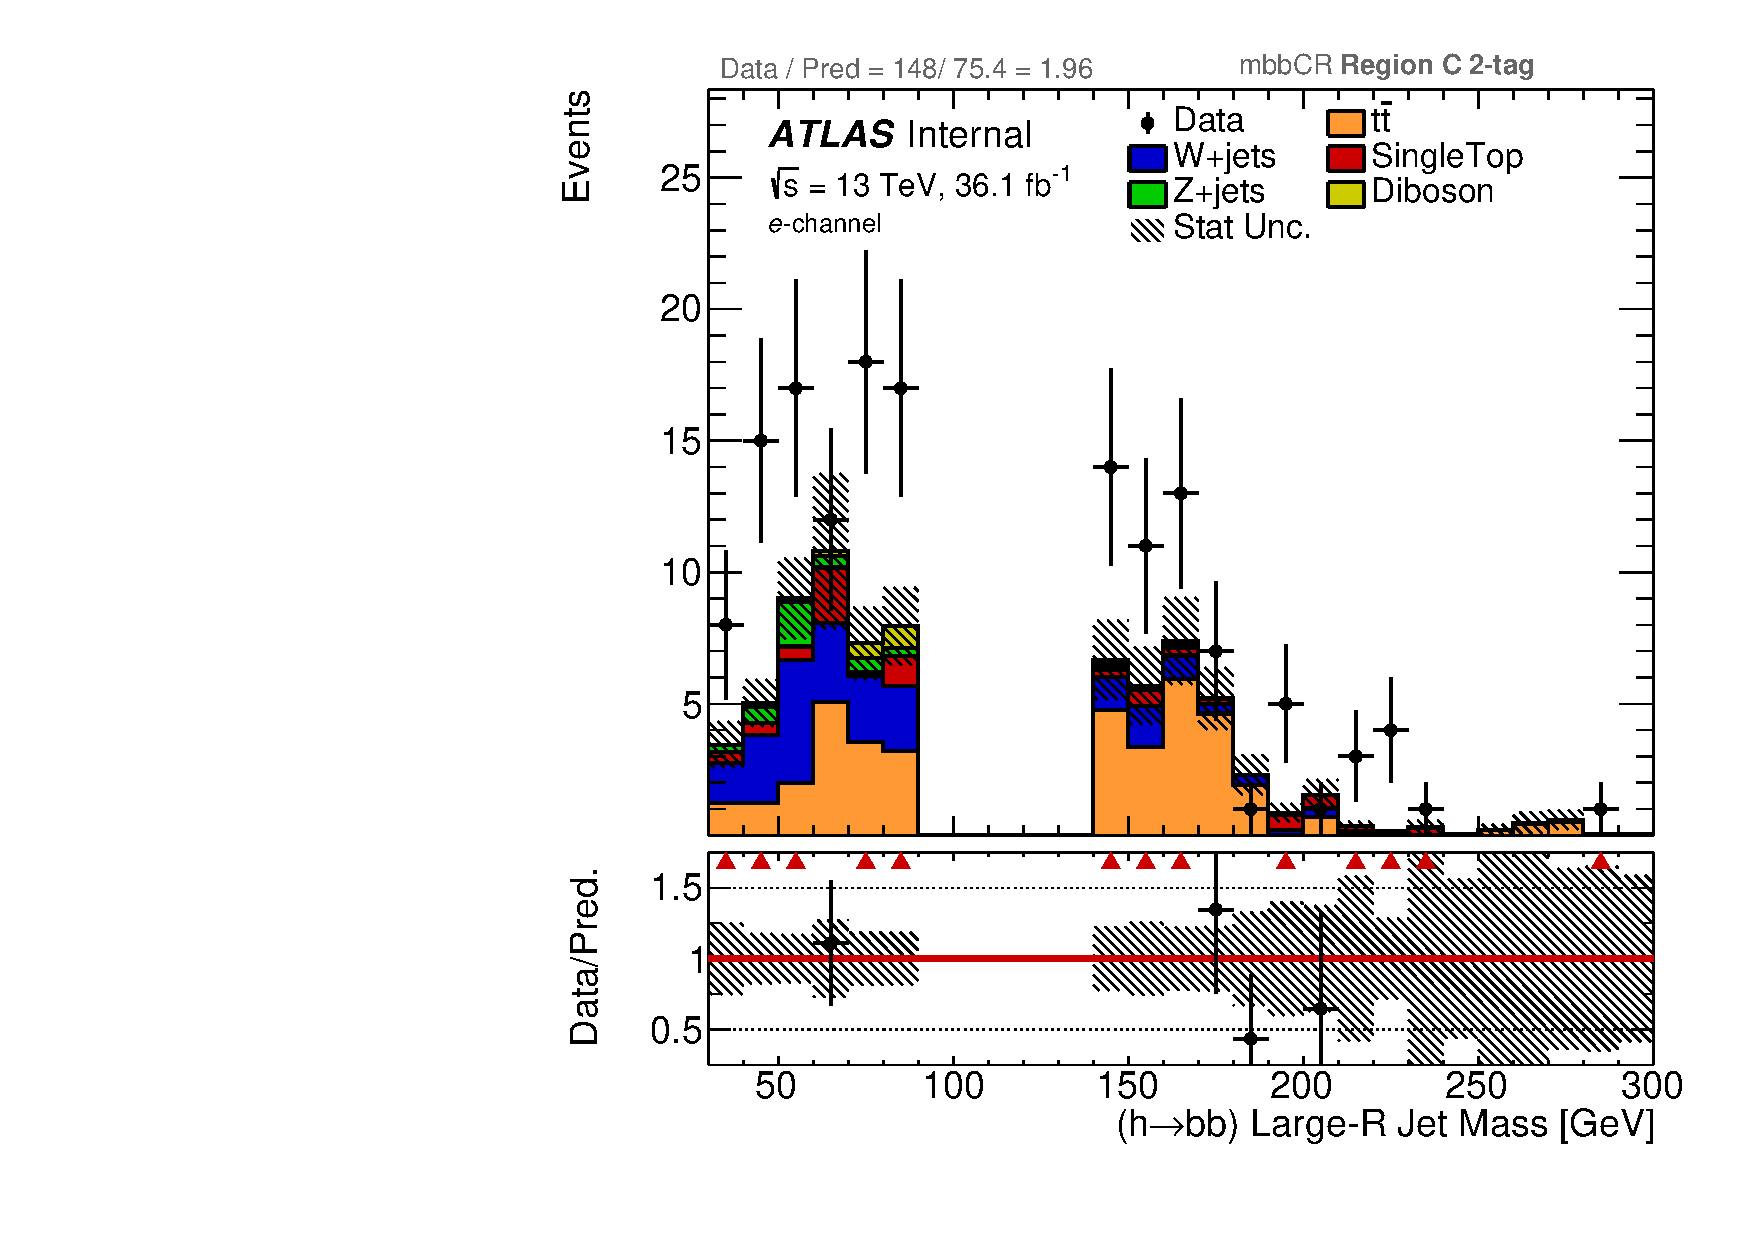
\includegraphics[scale=0.23]{./figures/boosted/ABCD/elec_mbbcr_RegionC_HbbMass} 
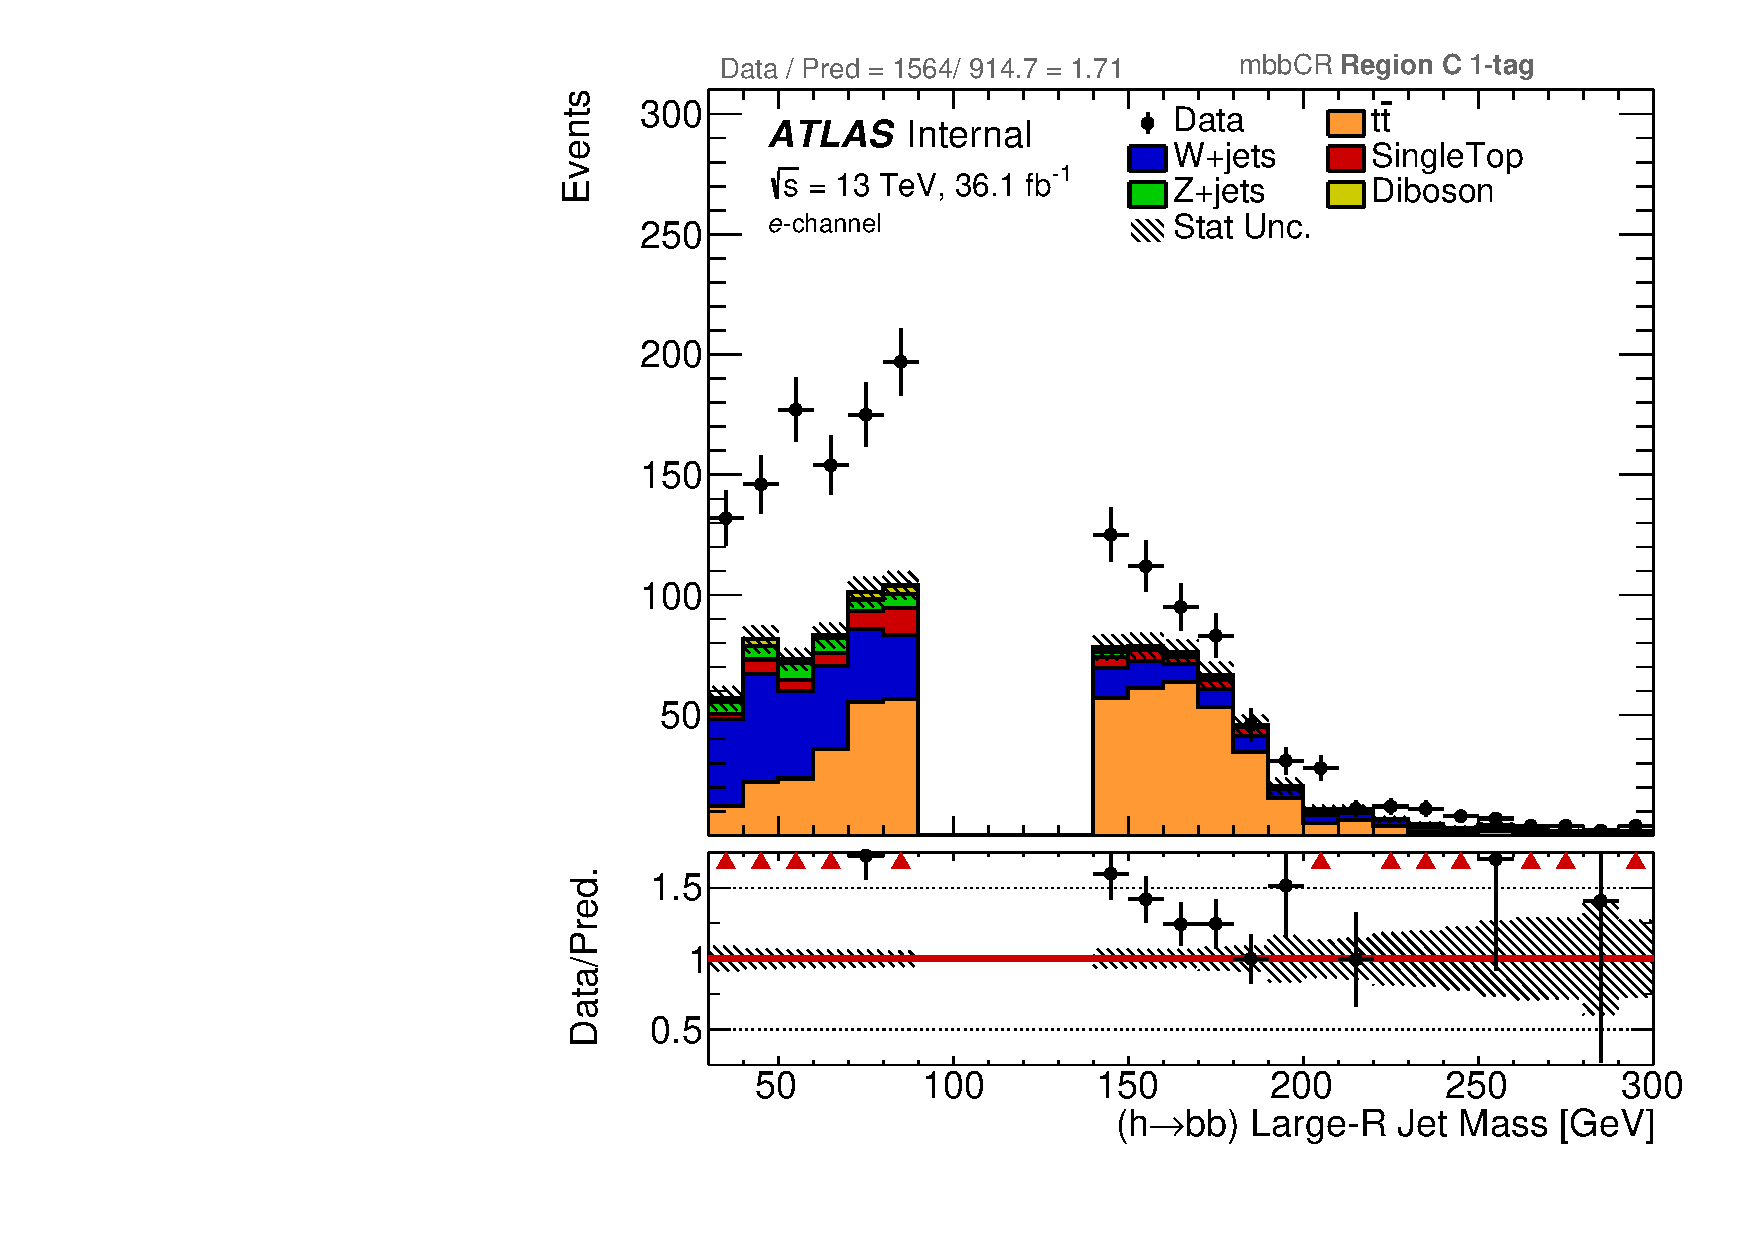
\includegraphics[scale=0.23]{./figures/boosted/ABCD/elec_mbbcr_RegionC_1tag_HbbMass}\\
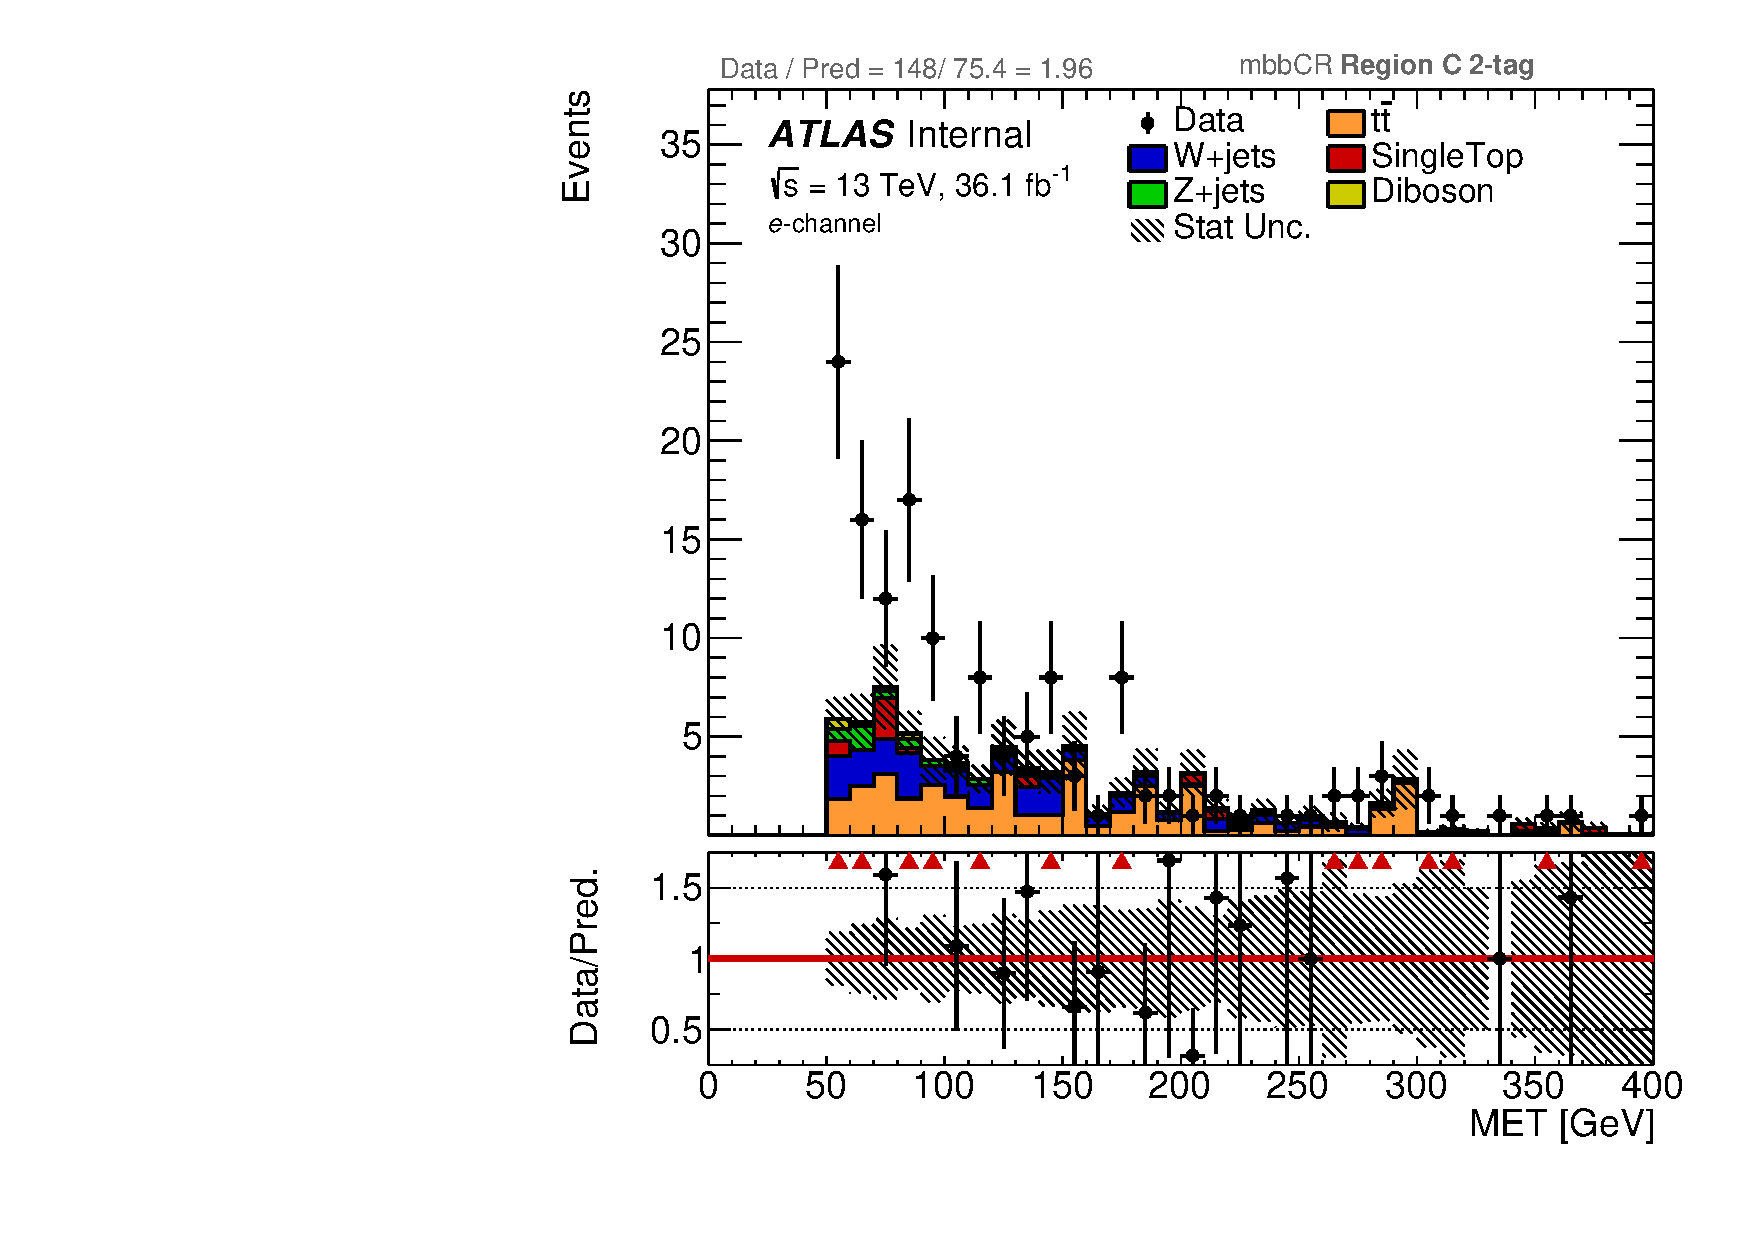
\includegraphics[scale=0.23]{./figures/boosted/ABCD/elec_mbbcr_RegionC_MET}
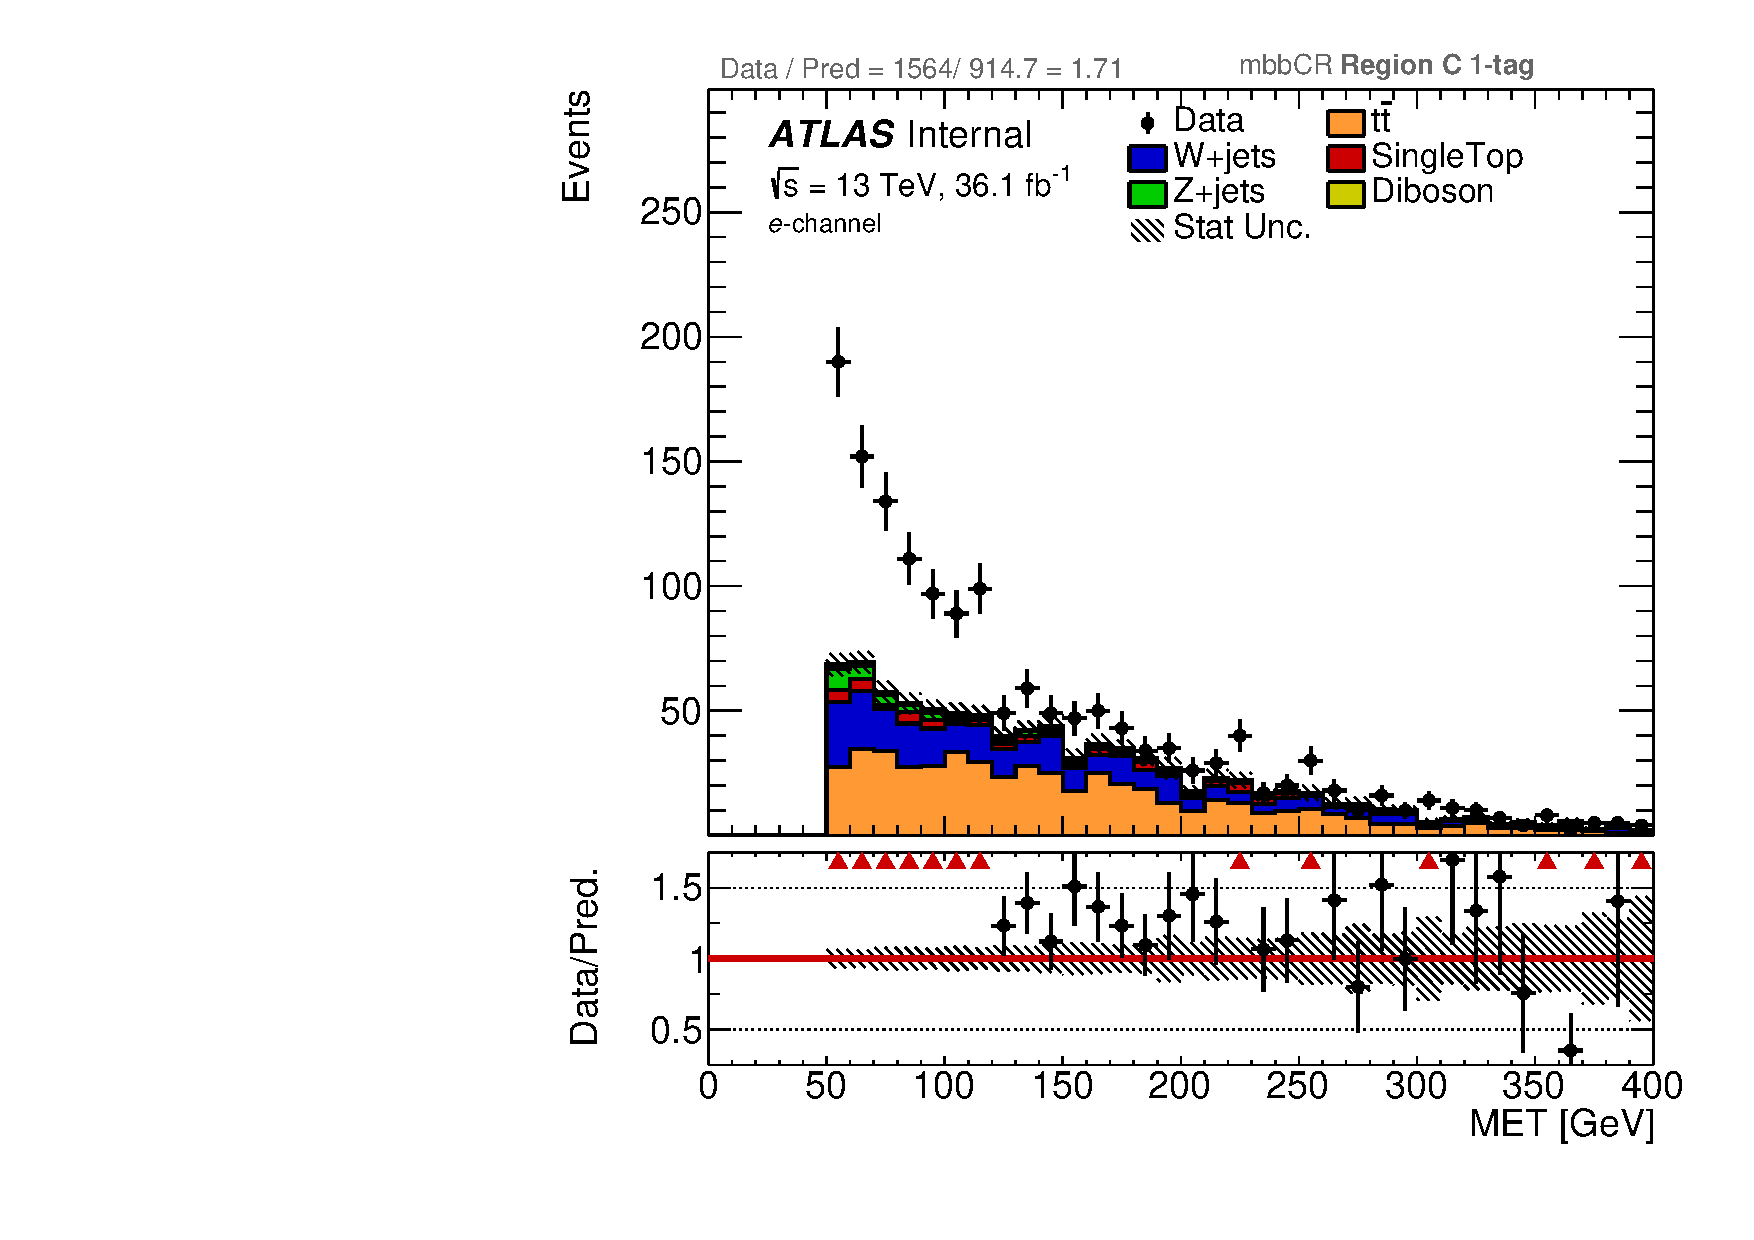
\includegraphics[scale=0.23]{./figures/boosted/ABCD/elec_mbbcr_RegionC_1tag_MET}\\
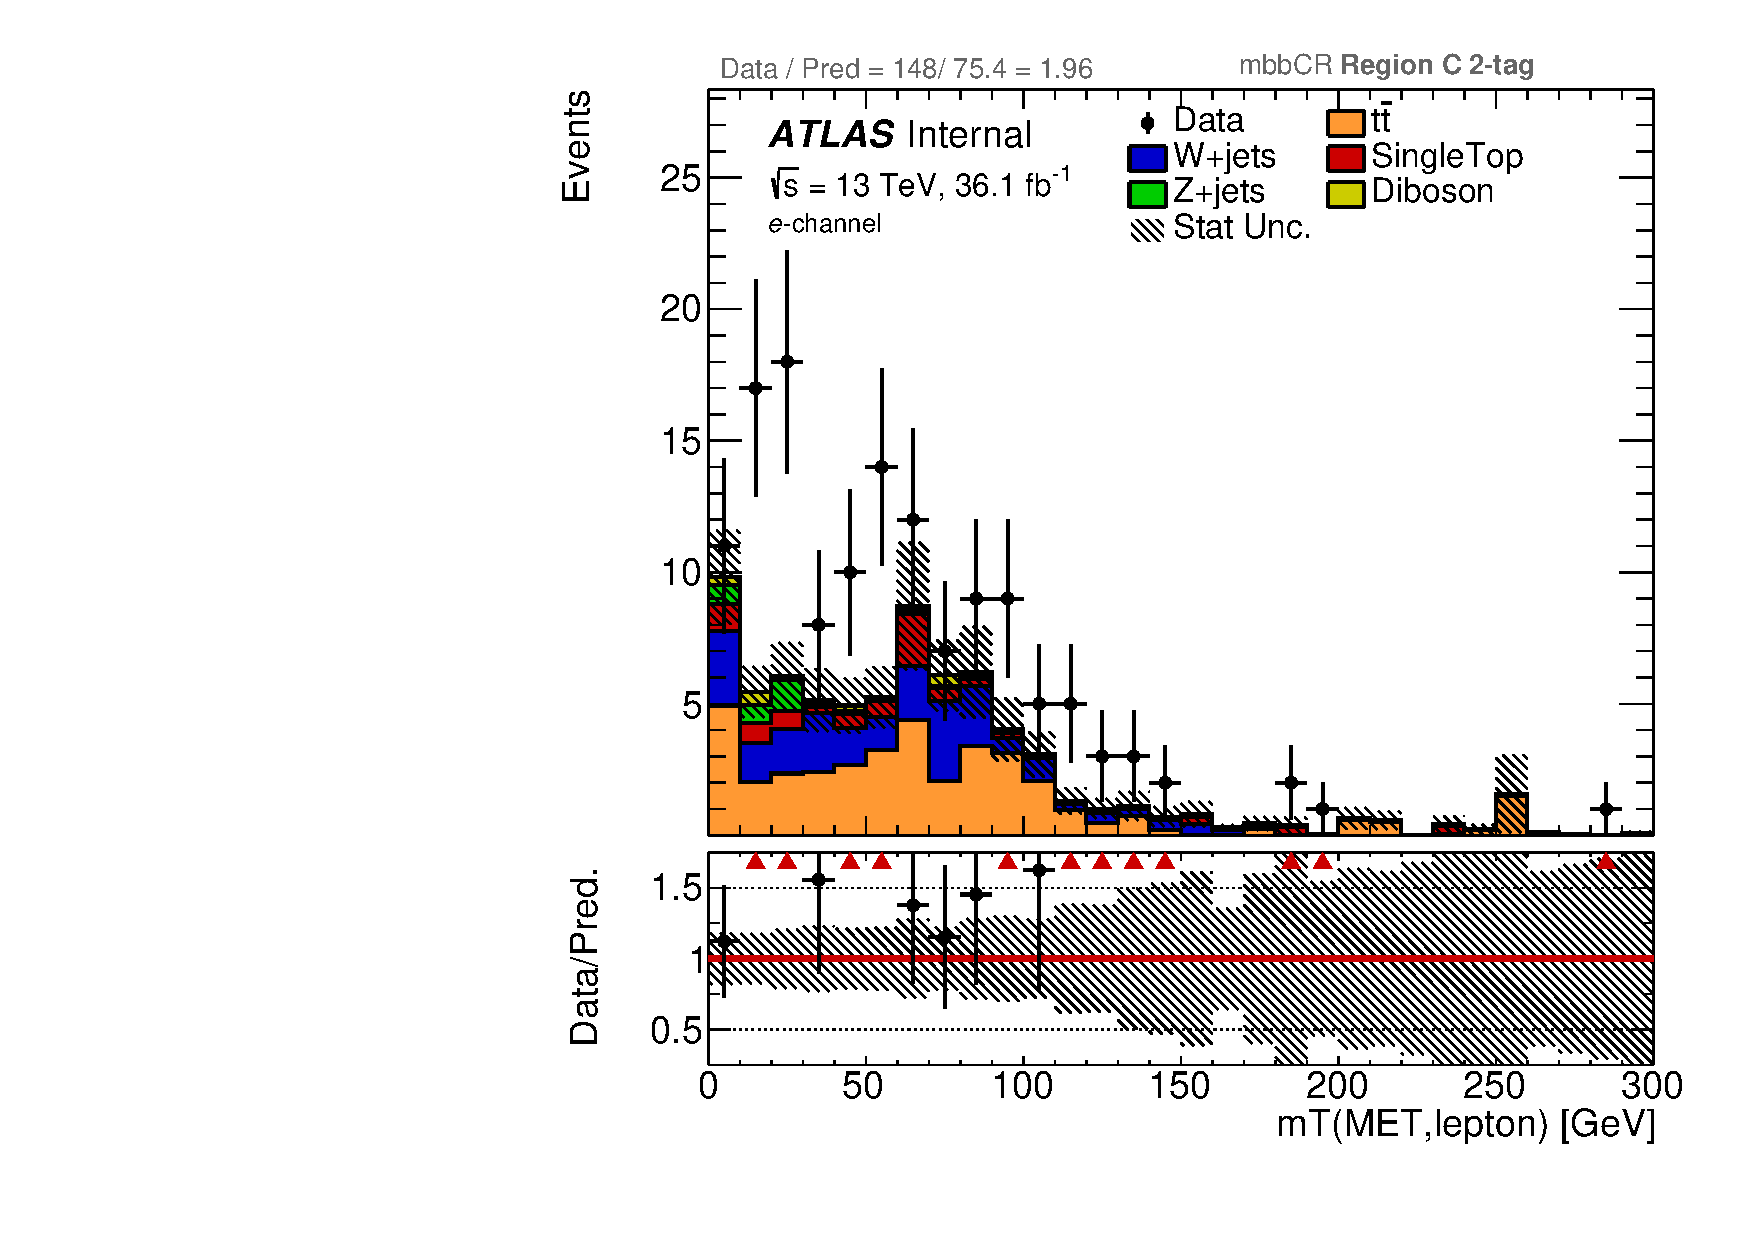
\includegraphics[scale=0.23]{./figures/boosted/ABCD/elec_mbbcr_RegionC_WlepMtATLAS}
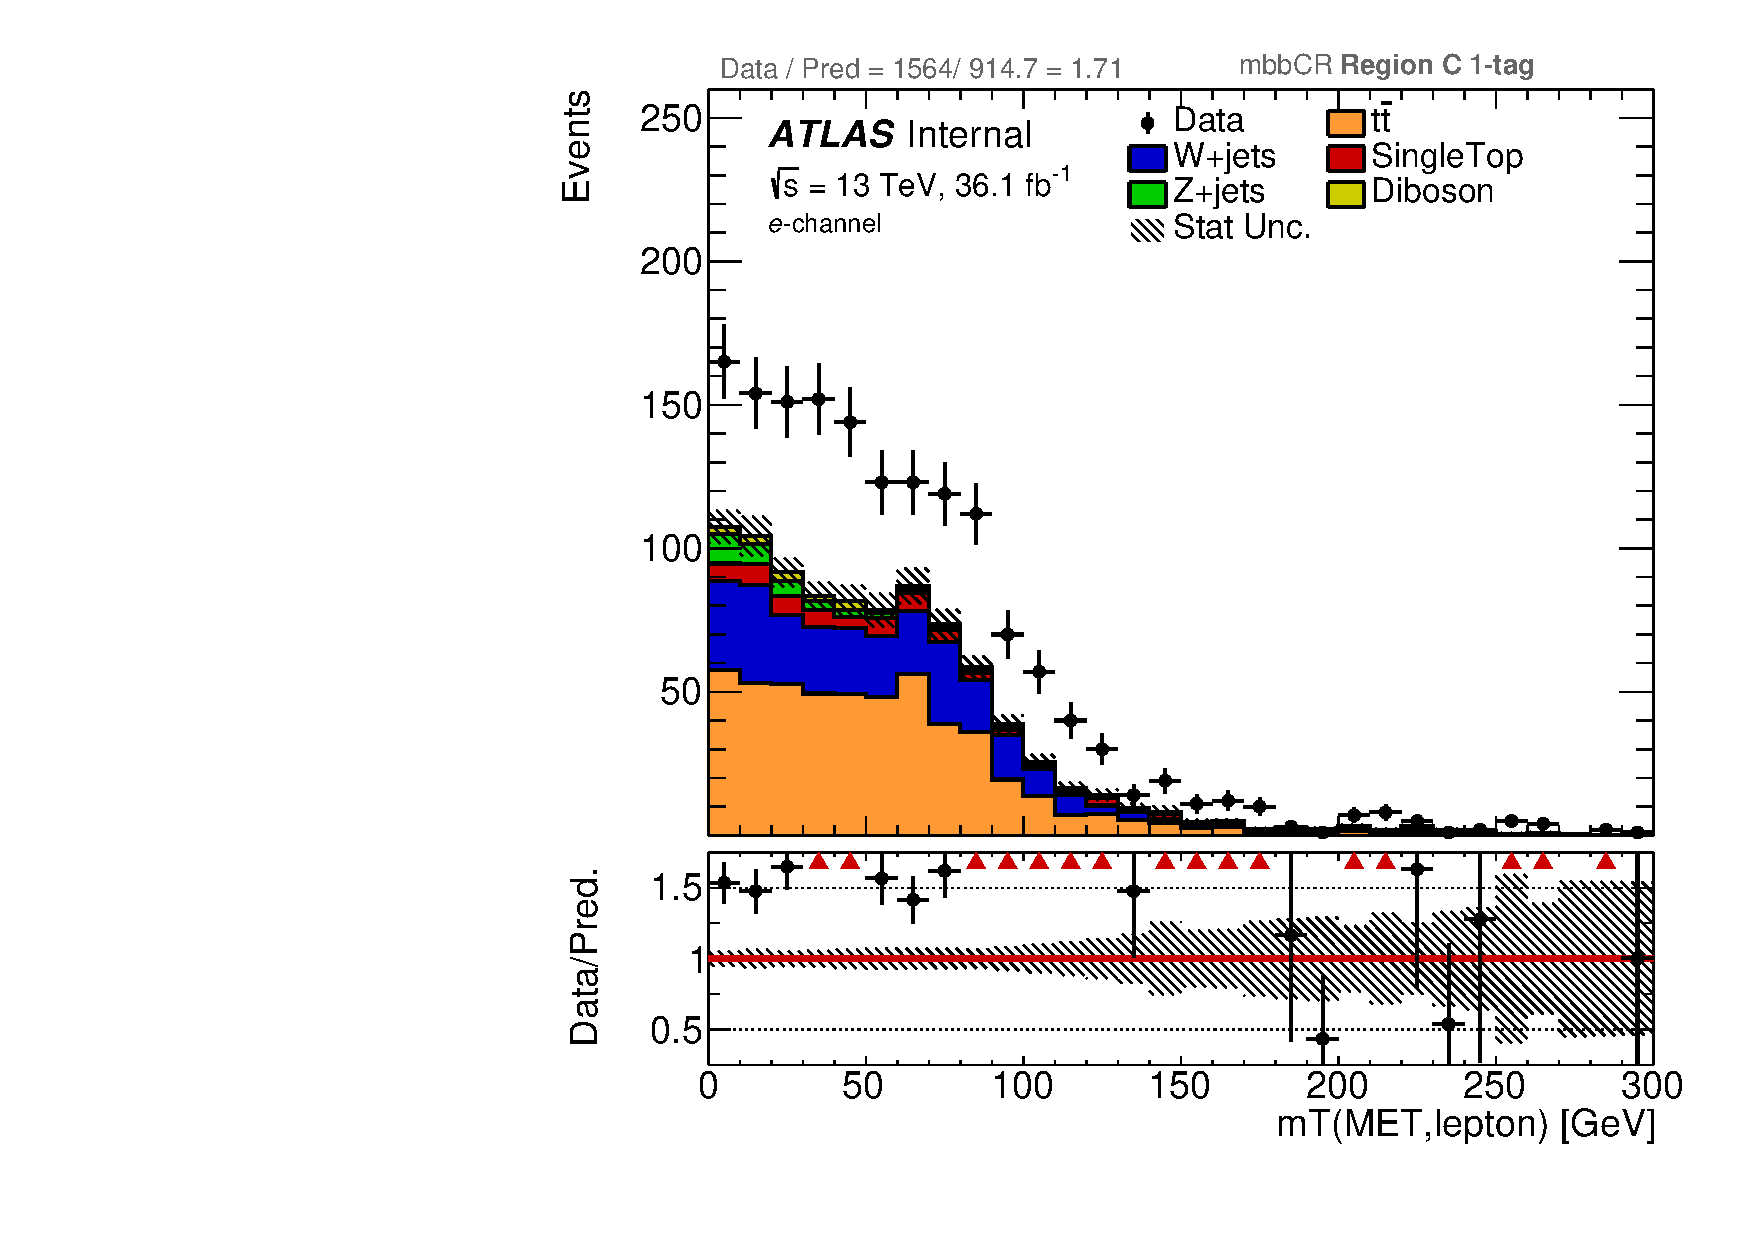
\includegraphics[scale=0.23]{./figures/boosted/ABCD/elec_mbbcr_RegionC_1tag_WlepMtATLAS}\\
\includegraphics[scale=0.23]{./figures/boosted/ABCD/elec_mbbcr_RegionC_hhMass}
\includegraphics[scale=0.23]{./figures/boosted/ABCD/elec_mbbcr_RegionC_1tag_hhMass}
\caption{Kinematic distributions in ABCD method region C of 2-tag events (left) and 1-tag events (right) in the electron channel mBBcr.}
\label{fig:boosted_abcd_region_c_mbbcr_elec}
\end{center}
\end{figure}

\begin{figure}[!htbp]
\begin{center}
\includegraphics[scale=0.23]{./figures/boosted/ABCD/muon_SR_RegionC_HbbMass}
\includegraphics[scale=0.23]{./figures/boosted/ABCD/muon_SR_RegionC_1tag_HbbMass}\\
\includegraphics[scale=0.23]{./figures/boosted/ABCD/muon_SR_RegionC_MET}
\includegraphics[scale=0.23]{./figures/boosted/ABCD/muon_SR_RegionC_1tag_MET}\\
\includegraphics[scale=0.23]{./figures/boosted/ABCD/muon_SR_RegionC_WlepMtATLAS}
\includegraphics[scale=0.23]{./figures/boosted/ABCD/muon_SR_RegionC_1tag_WlepMtATLAS}\\
\includegraphics[scale=0.23]{./figures/boosted/ABCD/muon_SR_RegionC_hhMass}
\includegraphics[scale=0.23]{./figures/boosted/ABCD/muon_SR_RegionC_1tag_hhMass}
\caption{Kinematic distributions in ABCD method region C of 2-tag events (left) and 1-tag events (right) in the muon channel SR.}
\label{fig:boosted_abcd_region_c_SR_muon}
\end{center}
\end{figure}

\begin{figure}[!htbp]
\begin{center}
\includegraphics[scale=0.23]{./figures/boosted/ABCD/elec_SR_RegionC_HbbMass}
\includegraphics[scale=0.23]{./figures/boosted/ABCD/elec_SR_RegionC_1tag_HbbMass}\\
\includegraphics[scale=0.23]{./figures/boosted/ABCD/elec_SR_RegionC_MET}
\includegraphics[scale=0.23]{./figures/boosted/ABCD/elec_SR_RegionC_1tag_MET}\\
\includegraphics[scale=0.23]{./figures/boosted/ABCD/elec_SR_RegionC_WlepMtATLAS}
\includegraphics[scale=0.23]{./figures/boosted/ABCD/elec_SR_RegionC_1tag_WlepMtATLAS}\\
\includegraphics[scale=0.23]{./figures/boosted/ABCD/elec_SR_RegionC_hhMass}
\includegraphics[scale=0.23]{./figures/boosted/ABCD/elec_SR_RegionC_1tag_hhMass}
\caption{Kinematic distributions in ABCD method region C of 2-tag events (left) and 1-tag events (right) in the electron channel SR.}
\label{fig:boosted_abcd_region_c_SR_elec}
\end{center}
\end{figure}

\begin{figure}[!htbp]
\begin{center}
\includegraphics[scale=0.33]{./figures/boosted/ABCD/muon_mbbcr_RegionC_Lep_d0sigL}     
\includegraphics[scale=0.33]{./figures/boosted/ABCD/muon_mbbcr_RegionC_1tag_Lep_d0sigL} \\
\includegraphics[scale=0.33]{./figures/boosted/ABCD/muon_SR_RegionC_Lep_d0sigL}         
\includegraphics[scale=0.33]{./figures/boosted/ABCD/muon_SR_RegionC_1tag_Lep_d0sigL}   \\
\caption{$|d_{0}^{\textrm{sig}}|$ distributions in ABCD method region C of 2-tag events (left) and 1-tag events (right) in the muon channel.}
\label{fig:boosted_abcd_region_c_SR_muon_d0}
\end{center}
\end{figure}

\begin{figure}[!htbp]
\begin{center}
\includegraphics[scale=0.33]{./figures/boosted/ABCD/elec_mbbcr_RegionC_Lep_d0sigL}        
\includegraphics[scale=0.33]{./figures/boosted/ABCD/elec_mbbcr_RegionC_1tag_Lep_d0sigL}  \\
\includegraphics[scale=0.33]{./figures/boosted/ABCD/elec_SR_RegionC_Lep_d0sigL}         
\includegraphics[scale=0.33]{./figures/boosted/ABCD/elec_SR_RegionC_1tag_Lep_d0sigL}    \\
\caption{$|d_{0}^{\textrm{sig}}|$ distributions in ABCD method region C of 2-tag events (left) and 1-tag events (right) in the electron channel.}
\label{fig:boosted_abcd_region_c_SR_elec_d0}
\end{center}
\end{figure}


\FloatBarrier
%%%%%%%%%%%%%%%%%%%%%%%%
%
% d0 variation studies
%
%%%%%%%%%%%%%%%%%%%%%%%
\subsection{Stability test: $|d_{0}^{\textrm{sig}}|$ cut variation.}
\label{app:boosted_qcd_d0variation}
The $|d_{0}^{\textrm{sig}}|$ cut value used in this analysis
is arbitrarily chosen to be 2.0 in order to use the ABCD method to estimate multijet background.
This cut value is chosen such that reasonable statistics are available in region C and region D.
As a stability test of the ABCD method to predict the multijet yield in region A,
the $|d_{0}^{\textrm{sig}}|$ cut value is varied by $\pm$ 1 from the baseline cut value of 2 
and the resulting multijet yield prediction for each $|d_{0}^{\textrm{sig}}|$ cut value variation
is compared to the baseline multijet yield prediction.Table~\ref{tab:boosted_syst_qcd_norm_d0cut} 
shows the predicted multijet yield in region A obtained by the ABCD method for different values of 
the $|d_{0}^{\textrm{sig}}|$ cut. 

\begin{table}[!htbp]
\begin{center}
\begin{tabular}{l|c|c}
$|d_{0}^{\textrm{sig}}|$ cut value     & Electron       & Muon        \\
\hline        
\multicolumn{3}{c}{SR} \\
\hline
< 2.0  (Baseline)       & 165.9 $\pm$ 46.6              & 69.3 $\pm$ 27.7 \\
< 1.0                   & 53.3  $\pm$ 16.3 [-67.9\%]    & 49.4 $\pm$ 21.9 [-28.7\%] \\  
< 3.0                   & 136.7 $\pm$ 61.6 [-17.6\%]    & 71.3 $\pm$ 40.0 [+2.9\%] \\    
\hline 
\multicolumn{3}{c}{mBBcr} \\
\hline
< 2.0 (Baseline)       & 277.1 $\pm$ 66.0             & 100.8 $\pm$ 41.3 \\
< 1.0                  & 138.9 $\pm$ 29.3  [-49.9\%]  & 82.2 $\pm$ 35.2 [-18.5\%]  \\          
< 3.0                  & 437.0 $\pm$ 123.1 [+57.7\%]  & 71.6 $\pm$ 71.9 [-29.0\%] \\     
\end{tabular}
\end{center}
\caption{The predicted multijet yield in region A for different $|d_{0}^{\textrm{sig}}|$ cut values. 
Only the statistical uncertainty on the yield is shown. The $|d_{0}^{\textrm{sig}}|$ < 2.0 cut is 
the baseline value used in the analysis. The values in the square brackets are the relative difference 
of the predicted yield with an alternative $|d_{0}^{\textrm{sig}}|$ cut value with respect to the 
baseline yield prediction.}
\label{tab:boosted_syst_qcd_norm_d0cut}
\end{table}

\FloatBarrier
%%%%%%%%%%%%%%%%%%%%
%
% mBBcr fit studies
%
%%%%%%%%%%%%%%%%%%%%
\subsection{QCD multijet normalization fit studies in mBB control region.}
\label{app:boosted_qcd_float_2tag_mbbcr_fit}

As a cross-check on the prediction of the QCD multijet yield with the ABCD method, a conditional background-only
likelihood fit of the large-$R$ jet mass distribution in the mBB control region. The normalization of the QCD multijet background,
assigned as an unconstrained nuisance parameter in the likelihood, is allowed to float in the likelihood fit. 
The bin-by-bin background statistical uncertainties are included as additional nuisance parameters but no systematic uncertainties 
on the MC predicted backgrounds are included. The fit is performed separately in the electron channel and the muon channel.

Table~\ref{tab:boosted_qcdfitstudies_mBBcr_normfact} shows the obtained normalization factor
on the QCD mulijet background in the electron and muon channels. The post-fit QCD multijet normalization factor 
for the muon channel is 1.069 $\pm$ 0.329, which is consistent with 1.0 and within the error obtained
from the fit. As for the electron channel, the normalization factor is 0.676 $\pm$ 0.130, which is a significant
deviation from 1.0. As there is a clear deviation from 1.0 for the electron channel, we assign an additional QCD multijet 
normalization uncertainty of 32.4\% for the electron channel due to the relative difference of the normalization factor from 1.0 
obtained from the likelihood fit.

\begin{table}
\begin{center}
\begin{tabular}{c|c}
Channel  & QCD Normalization Factor  \\      
\hline
Electron &  0.676 $\pm$ 0.130 \\
Muon     &  1.069 $\pm$ 0.329 \\
\end{tabular}
\end{center}
\caption{Post-fit normalization factors for QCD multijet background obtained 
from the mBB control region only fit of the large-$R$ jet mass distribution
to the observed data in the electron channeland muon channel.} 
\label{tab:boosted_qcdfitstudies_mBBcr_normfact}
\end{table}

Table~\ref{tab:boosted_elec_mbbcr_qcd_fitresults} and~\ref{tab:boosted_muon_bkgd_mbbcr_qcd_fitresults} show
the pre-fit and post-fit yields for all backgrounds and also the total yield of all backgorunds in 
the electron channel and muon channel respectively. In both channels, the post-fit total background yields 
are closer in agreement with the observed data yields. The pre-fit and post-fit large-$R$ jet mass distribution 
are shown in Figure~\ref{fig:boostedabcd_mbbcr_elec_fit} and Figure~\ref{fig:boostedabcd_mbbcr_muon_fit}.

\begin{table}
\begin{center}
\begin{tabular}{l|c|c} 
Sample        &  Pre-fit &  Post-fit \\ 
\hline 
$t\bar{t}$    &  521.93 $\pm$ 0.02  &  528.33 $\pm$ 11.22   \\ 
W+Jets        &  281.38 $\pm$ 0.01  &  282.80 $\pm$ 6.51    \\ 
QCD           &  277.08 $\pm$ 0.03  &  187.67 $\pm$ 33.95   \\ 
Single-top    &  81.58  $\pm$ 0.00  &  83.15  $\pm$ 1.73    \\ 
Z+Jets        &  27.12  $\pm$ 0.00  &  27.32  $\pm$ 0.62    \\ 
Dibosons      &  19.64  $\pm$ 0.00  &  19.84  $\pm$ 0.54    \\ 
\hline 
Prediction    &  1208.73 $\pm$ 0.04  & 1129.11 $\pm$ 31.22  \\ 
Data          &  1151                & 1151                 \\ 
\hline 
Data/Pred     &  0.952  &   1.019 \\ 
\hline 
\end{tabular} 
\end{center}
\caption{Prefit and postfit background yields and observed data yields in the mBB control region in the electron channel.}
\label{tab:boosted_elec_mbbcr_qcd_fitresults}
\end{table}

\begin{table}
\begin{center}
\begin{tabular}{l|c|c} 
Sample        &  Pre-fit &  Post-fit \\ 
\hline 
$t\bar{t}$    & 483.64 $\pm$ 0.01 &   488.67 $\pm$ 9.17     \\ 
W+Jets        & 284.25 $\pm$ 0.01 &   284.19 $\pm$ 5.55     \\ 
QCD           & 100.81 $\pm$ 0.01 &   107.75 $\pm$ 32.26    \\ 
Single-top    & 79.74  $\pm$ 0.00 &   79.97  $\pm$ 1.45     \\ 
Z+Jets        & 28.76  $\pm$ 0.00 &   28.74  $\pm$ 0.55     \\ 
Dibosons      & 20.07  $\pm$ 0.00 &   19.92  $\pm$ 0.45     \\ 
\hline 
Prediction    & 997.26 $\pm$ 0.03  &  1009.23 $\pm$ 29.89     \\ 
Data          & 1028               &  1028     \\ 
\hline 
Data/Pred     & 1.031 &   1.019   \\ 
\hline 
\end{tabular} 
\end{center}
\caption{Prefit and postfit background yields and observed data yields in the mBB control region in the muon channel.}
\label{tab:boosted_muon_bkgd_mbbcr_qcd_fitresults}
\end{table}

\begin{figure}[!htbp]
\begin{center}
\includegraphics[scale=0.33]{./figures/boosted/CR_QCDFloat_El/QCDFloat_mBBcr_El_Prefit} 
\includegraphics[scale=0.33]{./figures/boosted/CR_QCDFloat_El/QCDFloat_mBBcr_El_Postfit}\\
\caption{Prefit and postfit large-$R$ jet mass distribution in the mBB control region in the electron channel.}
\label{fig:boostedabcd_mbbcr_elec_fit}
\end{center}
\end{figure}

\begin{figure}[!htbp]
\begin{center}
\includegraphics[scale=0.33]{./figures/boosted/CR_QCDFloat_Mu/QCDFloat_mBBcr_Mu_Prefit} 
\includegraphics[scale=0.33]{./figures/boosted/CR_QCDFloat_Mu/QCDFloat_mBBcr_Mu_Postfit}\\
\caption{Prefit and postfit large-$R$ jet mass distribution in the mBB control region in the muon channel.}
\label{fig:boostedabcd_mbbcr_muon_fit}
\end{center}
\end{figure}


\FloatBarrier
%%%%%%%%%%%%%%%%%%%%
%
% ABCD 1-tag
%
%%%%%%%%%%%%%%%%%%%%
\subsection{ABCD method in 1-tag region.}
\label{app:boosted_abcd_1tag}
The ABCD method (Sec.\ref{sec:boosted_bkgd_qcdmultijet}) is repeated for events with exactly one $b$-tagged track-jet
in the large-$R$ jet. Events that fulfills this requirement is considered to be in the "1-tag" region and it is orthogonal 
to the 2-tag region. The 1-tag region can be used as a control region to assess background modelling in the signal region
($90~\GeV < m_\text{Large-R jet} < 140~\GeV$) as this region is overwhelmed with SM background processes and it is not expected to
be sensitive to signals. 

Table~\ref{tab:boosted_bkgd_1tag0bjet_abcd_ratio} shows the $\frac{N_B^\text{QCD}}{N_D^\text{QCD}}$ ratio in the electron channel and muon channel. 
The ratio in the electron channel is calculated to be 2.9 $\pm$ 0.2, which is as expected be larger than 1 as $N_B^\text{QCD}$ > $N_D^\text{QCD}$.
Interestingly, the ratio in the muon channel is less than 1. The dominant source of QCD multijet background for the muon channel is non-prompt muons 
from heavy-flavour hadron decays and the $|d_{0}^{\textrm{sig}}|$ $<$ 2.0 cut, which defines both region A (\met > 50 GeV) and region B (\met < 50 GeV), 
is effective in removing QCD multijet events which populate region D. Figure~\ref{fig:boosted_abcd_1tag0bjet_region_bd_muon} 
and~\ref{fig:boosted_abcd_1tag0bjet_region_bd_elec} show several kinematic distributions in region B and region D for the muon 
channel and electron channel respectively.

\begin{table}[!htbp]
\begin{center}
\begin{tabular}{l|c|c}
Multijet yield in region                & Electron                   & Muon \\        
\hline
$N_B^\text{QCD}$                        & 2790.1 $\pm$ 106.5 (3.8\%) & 77.8  $\pm$ 89.5 (115.1\%) \\
$N_D^\text{QCD}$                        & 947.7  $\pm$ 38.5 (4.1\%)  & 493.1 $\pm$ 30.6 (6.2\%)   \\
\hline
$N_{B}^\text{QCD}$/$N_{D}^\text{QCD}$   & 2.9   $\pm$ 0.2 (5.6\%)    & 0.2   $\pm$ 0.2 (115.2\%)  \\
\end{tabular}
\end{center}
\caption{Multijet yields in 1-tag region B and 1-tag region D and also the ratio of the yields for each lepton channel. 
The error on the $\frac{N_B^\text{QCD}}{N_D^\text{QCD}}$ ratio is propagated from the statistical uncertainties 
on the multijet yields in each region.}
\label{tab:boosted_bkgd_1tag0bjet_abcd_ratio}
\end{table}

\begin{figure}[!htbp]
\begin{center}
\includegraphics[scale=0.33]{./figures/boosted/ABCD_1tag0bjet/elec_Inc_RegionB_HbbMass}
\includegraphics[scale=0.33]{./figures/boosted/ABCD_1tag0bjet/elec_Inc_RegionD_HbbMass}\\
\includegraphics[scale=0.33]{./figures/boosted/ABCD_1tag0bjet/elec_Inc_RegionB_MET}  
\includegraphics[scale=0.33]{./figures/boosted/ABCD_1tag0bjet/elec_Inc_RegionD_MET}    \\
\includegraphics[scale=0.33]{./figures/boosted/ABCD_1tag0bjet/elec_Inc_RegionB_WlepMtATLAS}
\includegraphics[scale=0.33]{./figures/boosted/ABCD_1tag0bjet/elec_Inc_RegionD_WlepMtATLAS}\\
\includegraphics[scale=0.33]{./figures/boosted/ABCD_1tag0bjet/elec_Inc_RegionB_hhMass}    
\includegraphics[scale=0.33]{./figures/boosted/ABCD_1tag0bjet/elec_Inc_RegionD_hhMass}    
\caption{Kinematic distributions in ABCD method region B (left) and region D (right) in the electron channel.
Only statistical uncertainty on the background prediction is included.}
\label{fig:boosted_abcd_1tag0bjet_region_bd_elec}
\end{center}
\end{figure}

\begin{figure}[!htbp]
\begin{center}
\includegraphics[scale=0.33]{./figures/boosted/ABCD_1tag0bjet/muon_Inc_RegionB_HbbMass}
\includegraphics[scale=0.33]{./figures/boosted/ABCD_1tag0bjet/muon_Inc_RegionD_HbbMass}\\
\includegraphics[scale=0.33]{./figures/boosted/ABCD_1tag0bjet/muon_Inc_RegionB_MET}    
\includegraphics[scale=0.33]{./figures/boosted/ABCD_1tag0bjet/muon_Inc_RegionD_MET}   \\
\includegraphics[scale=0.33]{./figures/boosted/ABCD_1tag0bjet/muon_Inc_RegionB_WlepMtATLAS}
\includegraphics[scale=0.33]{./figures/boosted/ABCD_1tag0bjet/muon_Inc_RegionD_WlepMtATLAS}\\
\includegraphics[scale=0.33]{./figures/boosted/ABCD_1tag0bjet/muon_Inc_RegionB_hhMass}  
\includegraphics[scale=0.33]{./figures/boosted/ABCD_1tag0bjet/muon_Inc_RegionD_hhMass}   
\caption{Kinematic distributions in ABCD method region B (left) and region D (right) in the muon channel.
Only statistical uncertainty on the background prediction is included.}
\label{fig:boosted_abcd_1tag0bjet_region_bd_muon}
\end{center}
\end{figure}

Table~\ref{tab:boosted_bkgd_1tag0bjet_abcd_yield} shows the 1-tag signal region and 1-tag mBB control region QCD 
multijet yield in region C ($N_C^\text{QCD}$) and the predicted QCD multijet yield in region A ($N_A^\text{QCD}$) 
of the 1-tag mBB control region and 1-tag signal region for both lepton channels. $N_A^\text{QCD}$ is predicted by 
scaling $N_C^\text{QCD}$ with the $\frac{N_B^\text{QCD}}{N_D^\text{QCD}}$ ratio. The QCD multijet background shape 
prediction in 1-tag region A is derived from QCD background shape templates in 1-tag region C.

\begin{table}[!htbp]
\begin{center}
\begin{tabular}{c|c|c}
Multijet yield in region & Electron & Muon  \\  
\hline
\multicolumn{3}{c}{SR} \\
\hline
$N_C^\text{QCD}$         & 299.9 $\pm$ 30.9 (10.3\%)          & 246.7 $\pm$ 29.1 (11.8\%)  \\
$N_A^\text{QCD}$         & 882.9 $\pm$ 103.3 (11.7\%)         & 38.9 $\pm$ 45.1 (115.8\%)  \\
\hline
\multicolumn{3}{c}{mBBcr} \\
\hline
$N_C^\text{QCD}$       & 649.3 $\pm$ 43.5 (6.7\%)           & 637.2 $\pm$ 40.6 (6.4\%)     \\
$N_A^\text{QCD}$       & 1911.6 $\pm$ 166.5 (8.7\%)         & 100.6 $\pm$ 116.1 (115.4\%)  \\
\hline
\end{tabular}
\end{center}
\caption{Multijet yield in region C and predicted yield in region A in the signal region. The error on $N_A^\text{QCD}$
are propagated from the error on the $N_B^\text{QCD}$/$N_B^\text{QCD}$ ratio and statistical uncertainty on $N_C^\text{QCD}$ yield.
The numbers in brackets are the relative uncertainty in percentage.} 
\label{tab:boosted_bkgd_1tag0bjet_abcd_yield}
\end{table}

The predicted backgrounds and observed data yields in region A of the 1-tag signal region are shown 
in Table~\ref{tab:boosted_bkgd_1tag0bjet_abcd_a_SR}. The overestimation of the total predicted background
in the electron channel after the QCD multijet prediction is included into the total prediction suggests
that the QCD background is overestimated. The same observation can be made in the 1-tag mBB control region as 
shown in Table~\ref{tab:boosted_bkgd_1tag0bjet_abcd_a_mbbcr}.Figure~\ref{fig:boosted_abcd_1tag0bjet_region_a_withqcd_SR},
~\ref{fig:boosted_abcd_1tag0bjet_region_a_withqcd_SR} and~\ref{fig:boosted_abcd_1tag0bjet_region_a_withqcd_lepton} show 
several kinematic variables in the region A 1-tag signal region and 1-tag mBB control region for the electron, muon and 
combined lepton channel.

\renewcommand{\arraystretch}{1.5}
\begin{table}
\begin{center}
\begin{tabular}{l|c|c|c}
Sample            & Electron       & Muon      & Combined     \\ 
\hline
$t\bar{t}$        & 3940.21 $^{+517.0(+13.1\%)}_{-531.7(-13.5\%)}$  & 3784.69 $^{+522.0(+13.8\%)}_{-484.6(-12.8\%)}$ & 7724.90 $^{+1035.8(+13.4\%)}_{-1013.2(-13.1\%)}$ \\
W+jets            & 1205.12 $^{+331.8(+27.5\%)}_{-330.3(-27.4\%)}$  & 1256.88 $^{+341.0(+27.1\%)}_{-354.8(-28.2\%)}$ & 2462.00 $^{+671.3(+27.3\%)}_{-684.5(-27.8\%)}$   \\
Z+jets            & 105.13  $^{+29.5(+28.1\%)}_{-27.6(-26.2\%)}$    & 116.32  $^{+32.0(+27.5\%)}_{-32.4(-27.9\%)}$   & 221.45  $^{+60.9(+27.5\%)}_{-59.8(-27.0\%)}$     \\
SingleTop         & 322.68  $^{+43.7(+13.5\%)}_{-35.6(-11.0\%)}$    & 281.45  $^{+38.3(+13.6\%)}_{-33.5(-11.9\%)}$   & 604.13  $^{+81.2(+13.4\%)}_{-67.9(-11.2\%)}$     \\
Dibosons          & 80.18   $^{+39.2(+48.9\%)}_{-37.1(-46.3\%)}$    & 84.13   $^{+39.5(+46.9\%)}_{-39.5(-46.9\%)}$   & 164.31  $^{+77.9(+47.4\%)}_{-76.2(-46.4\%)}$     \\
QCD               & 882.92       & 38.94        & 921.86      \\
\hline
MCBkgd            & 5653.33 $^{+768.2(+13.6\%)}_{-759.3(-13.4\%)}$  & 5523.46 $^{+766.4(+13.9\%)}_{-742.3(-13.4\%)}$  & 11176.79 $^{+1531.2(+13.7\%)}_{-1497.8(-13.4\%)}$    \\
MCBkgd+QCD        & 6536.25      & 5562.40      & 12098.65    \\
Data              & 5645         & 4998         & 10643       \\
\hline
Data/MCBkgd       & 0.999        & 0.905        & 0.952       \\
Data/(MCBkgd+QCD) & 0.864        & 0.899        & 0.880       \\
\end{tabular}
\end{center}
\caption{Yields of various predicted backgrounds and observed data in the 1-tag signal region. "MCBkgd" consists
of all MC background samples with the exception of QCD which is predicted with the ABCD method. "MCBkgd+QCD" is 
the total yield of all backgrounds including QCD background. Only the detector modelling systematic uncertainties are taken
into account for the MC predicted backgrounds.}
\label{tab:boosted_bkgd_1tag0bjet_abcd_a_SR}
\end{table}
\renewcommand{\arraystretch}{1.0}

\renewcommand{\arraystretch}{1.5}
\begin{table}
\begin{center}
\begin{tabular}{l|c|c|c}
Sample           & Electron      & Muon        & Combined     \\ 
\hline
$t\bar{t}$        & 6399.98 $^{+772.8(+12.1\%)}_{-767.6(-12.0\%)}$  & 6026.35 $^{+729.4(+12.1\%)}_{-736.9(-12.2\%)}$  & 12426.32   $^{+1498.6(+12.1\%)}_{-1499.8(-12.1\%)}$  \\
W+jets            & 3138.83 $^{+903.0(+28.8\%)}_{-923.5(-29.4\%)}$  & 3203.21 $^{+926.5(+28.9\%)}_{-940.5(-29.4\%)}$  & 6342.04    $^{+1828.1(+28.8\%)}_{-1862.9(-29.4\%)}$  \\
Z+jets            & 270.43  $^{+76.6(+28.3\%)}_{-75.0(-27.7\%)}$    & 297.69  $^{+84.6(+28.4\%)}_{-81.4(-27.3\%)}$    & 568.12     $^{+160.3(+28.2\%)}_{-156.2(-27.5\%)}$  \\
SingleTop         & 636.26  $^{+60.7(+9.5\%)}_{-67.5(-10.6\%)}$     & 616.90  $^{+61.6(+10.0\%)}_{-63.1(-10.2\%)}$    & 1253.17    $^{+120.4(+9.6\%)}_{-129.5(-10.3\%)}$  \\
Dibosonsv221      & 174.97  $^{+80.9(+46.2\%)}_{-81.3(-46.5\%)}$    & 174.59  $^{+82.4(+47.2\%)}_{-82.8(-47.4\%)}$    & 349.56     $^{+163.0(+46.6\%)}_{-163.7(-46.8\%)}$  \\
QCD               & 1911.60      & 100.58       & 2012.18     \\
\hline
MCBkgd            & 10620.46 $^{+1475.7(+13.9\%)}_{-1497.0(-14.1\%)}$  & 10318.74 $^{+1472.8(+14.3\%)}_{-1485.0(-14.4\%)}$      & 20939.20 $^{+2942.8(+14.1\%)}_{-2976.1(-14.2\%)}$  \\
MCBkgd+QCD        & 12532.06     & 10419.32     & 22951.38    \\
Data              & 11225        & 9781         & 21006       \\
\hline
Data/MCBkgd       & 1.057        & 0.948        & 1.003       \\
Data/(MCBkgd+QCD) & 0.896        & 0.939        & 0.915       \\
\end{tabular}
\end{center}
\caption{Yields of various predicted backgrounds and observed data in the 1-tag mBB control region. "MCBkgd" consists
of all MC background samples with the exception of QCD which is predicted with the ABCD method. "MCBkgd+QCD" is 
the total yield of all backgrounds including QCD background.Only the detector modelling systematic uncertainties are taken
into account for the MC predicted backgrounds.}
\label{tab:boosted_bkgd_1tag0bjet_abcd_a_mbbcr}
\end{table}
\renewcommand{\arraystretch}{1.0}


\begin{figure}[!htbp]
\begin{center}
\includegraphics[scale=0.33]{./figures/boosted/ABCD_1tag0bjet/elec_SR_RegionA_HbbMass_withDD}
\includegraphics[scale=0.33]{./figures/boosted/ABCD_1tag0bjet/muon_SR_RegionA_HbbMass_withDD}\\
\includegraphics[scale=0.33]{./figures/boosted/ABCD_1tag0bjet/elec_SR_RegionA_MET_withDD}  
\includegraphics[scale=0.33]{./figures/boosted/ABCD_1tag0bjet/muon_SR_RegionA_MET_withDD}  \\
\includegraphics[scale=0.33]{./figures/boosted/ABCD_1tag0bjet/elec_SR_RegionA_WlepMtATLAS_withDD}
\includegraphics[scale=0.33]{./figures/boosted/ABCD_1tag0bjet/muon_SR_RegionA_WlepMtATLAS_withDD}\\
\includegraphics[scale=0.33]{./figures/boosted/ABCD_1tag0bjet/elec_SR_RegionA_hhMass_withDD} 
\includegraphics[scale=0.33]{./figures/boosted/ABCD_1tag0bjet/muon_SR_RegionA_hhMass_withDD}    
\caption{Kinematic distributions in 1-tag signal region (ABCD method) region A in the electron channel (left) and muon channel (right) with QCD multijet
background prediction included. Only statistical uncertainty on the background prediction is included.}
\label{fig:boosted_abcd_1tag0bjet_region_a_withqcd_SR}
\end{center}
\end{figure}

\begin{figure}[!htbp]
\begin{center}
\includegraphics[scale=0.33]{./figures/boosted/ABCD_1tag0bjet/elec_mbbcr_RegionA_HbbMass_withDD}
\includegraphics[scale=0.33]{./figures/boosted/ABCD_1tag0bjet/muon_mbbcr_RegionA_HbbMass_withDD}\\
\includegraphics[scale=0.33]{./figures/boosted/ABCD_1tag0bjet/elec_mbbcr_RegionA_MET_withDD}  
\includegraphics[scale=0.33]{./figures/boosted/ABCD_1tag0bjet/muon_mbbcr_RegionA_MET_withDD}  \\
\includegraphics[scale=0.33]{./figures/boosted/ABCD_1tag0bjet/elec_mbbcr_RegionA_WlepMtATLAS_withDD}
\includegraphics[scale=0.33]{./figures/boosted/ABCD_1tag0bjet/muon_mbbcr_RegionA_WlepMtATLAS_withDD}\\
\includegraphics[scale=0.33]{./figures/boosted/ABCD_1tag0bjet/elec_mbbcr_RegionA_hhMass_withDD}   
\includegraphics[scale=0.33]{./figures/boosted/ABCD_1tag0bjet/muon_mbbcr_RegionA_hhMass_withDD}     
\caption{Kinematic distributions in 1-tag mBB control region of (ABCD method) region A in the electron channel (left) and muon channel (right)
with QCD multijet background prediction included. Only statistical uncertainty on the background prediction is included.}
\label{fig:boosted_abcd_1tag0bjet_region_a_withqcd_mbbcr}
\end{center}
\end{figure}

\begin{figure}[!htbp]
\begin{center}
\includegraphics[scale=0.33]{./figures/boosted/ABCD_1tag0bjet/lepCombined_mbbcr_RegionA_HbbMass_withDD}  
\includegraphics[scale=0.33]{./figures/boosted/ABCD_1tag0bjet/lepCombined_SR_RegionA_HbbMass_withDD}       \\
\includegraphics[scale=0.33]{./figures/boosted/ABCD_1tag0bjet/lepCombined_mbbcr_RegionA_MET_withDD}  
\includegraphics[scale=0.33]{./figures/boosted/ABCD_1tag0bjet/lepCombined_SR_RegionA_MET_withDD}        \\
\includegraphics[scale=0.33]{./figures/boosted/ABCD_1tag0bjet/lepCombined_mbbcr_RegionA_WlepMtATLAS_withDD}
\includegraphics[scale=0.33]{./figures/boosted/ABCD_1tag0bjet/lepCombined_SR_RegionA_WlepMtATLAS_withDD} \\
\includegraphics[scale=0.33]{./figures/boosted/ABCD_1tag0bjet/lepCombined_mbbcr_RegionA_hhMass_withDD}   
\includegraphics[scale=0.33]{./figures/boosted/ABCD_1tag0bjet/lepCombined_SR_RegionA_hhMass_withDD}      
\caption{Kinematic distributions in 1-tag combined lepton channel (ABCD method) region A in the mBB control region (left) and signal region (right)
with QCD multijet background prediction included. Only statistical uncertainty on the background prediction is included.}
\label{fig:boosted_abcd_1tag0bjet_region_a_withqcd_lepton}
\end{center}
\end{figure}


\FloatBarrier
\subsubsection{QCD multijet normalization fit studies in signal and mBB control region.}
\label{app:boosted_qcd_float_1tag_SRmbbcr_fit}

A likelihood fit study, similar to what was presented in Appendix~\ref{app:boosted_qcd_float_2tag_mbbcr_fit}, is done for the 
1-tag region. The QCD multijet background is allowed to float in the likelihood fit and several likelihood fit scenarios are 
studied.

Table~\ref{tab:boosted_qcdfitstudies_1tag_normfact}list the post-fit multijet background normalization factor obtained 
from the likelihood fit with the signal region only fit, mBB control region only fit and the simultaneous fit of both regions
in each of the lepton channel. As in the previous appendix, the QCD normalization factors in all three fit scenarios suggests 
that the multijet background predicted with ABCD method is overestimated.

The pre-fit and post-fit (signal region only and mBB control region only) large-$R$ jet mass distributions 
for the electron channel and the muon channel are shown in Figure~\ref{fig:boostedabcd_mbbcrSRsepa_elec_fit} and~\ref{fig:boostedabcd_mbbcrSRsepa_muon_fit}
respectively. The pre-fit and post-fit large-$R$ jet mass distributions for the simultaneous fit in the signal and mBB control region are shown in 
in Figure~\ref{fig:boostedabcd_mbbcrSRsimul_elec_fit} and~\ref{fig:boostedabcd_mbbcrSRsimul_muon_fit}.


\begin{table}
\begin{center}
\begin{tabular}{c|c}
Channel  & QCD Normalization Factor  \\
\hline    
\multicolumn{2}{c}{SR only fit} \\
\hline
Electron &  0.02 $\pm$ 0.11 \\
Muon     &  3.02652$\times$10$^{-11}$  $\pm$  0.13438 \\
\hline    
\multicolumn{2}{c}{mBBcr only fit} \\
\hline
Electron &  0.46      $\pm$ 0.05 \\
Muon     &  3.31106$\times$10$^{-9}$  $\pm$  0.285013 \\
\hline    
\multicolumn{2}{c}{SR+mBBcr simultaneous fit} \\
\hline
Electron &  0.35  $\pm$ 0.04 \\
Muon     &  1.56074$\times$10$^{-6}$  $\pm$  0.0915855 \\
\end{tabular}
\end{center}
\caption{Post-fit normalization factors for QCD multijet background obtained 
from the 1-tag signalregion only fit, mBB control region only fit and simultaneous
fit of both regions of the large-$R$ jet mass distribution to the observed data 
in the electron channel and muon channel.} 
\label{tab:boosted_qcdfitstudies_1tag_normfact}
\end{table}

\begin{figure}[!htbp]
\begin{center}
\includegraphics[scale=0.33]{./figures/boosted/ABCD_1tag0bjet/QCDFloat_1tag_SRFit_SR_El_Prefit} 
\includegraphics[scale=0.33]{./figures/boosted/ABCD_1tag0bjet/QCDFloat_1tag_SRFit_SR_El_Postfit}\\
\includegraphics[scale=0.33]{./figures/boosted/ABCD_1tag0bjet/QCDFloat_1tag_mBBcrFit_mBBcr_El_Prefit} 
\includegraphics[scale=0.33]{./figures/boosted/ABCD_1tag0bjet/QCDFloat_1tag_mBBcrFit_mBBcr_El_Postfit}\\
\caption{Prefit and postfit large-$R$ jet mass distribution in the 1-tag signal and mBB control region in the electron channel. The fit is done separately
in the signal region (top) and mBB control region (bottom).}
\label{fig:boostedabcd_mbbcrSRsepa_elec_fit}
\end{center}
\end{figure}

\begin{figure}[!htbp]
\begin{center}
\includegraphics[scale=0.33]{./figures/boosted/ABCD_1tag0bjet/QCDFloat_1tag_SRFit_SR_Mu_Prefit}
\includegraphics[scale=0.33]{./figures/boosted/ABCD_1tag0bjet/QCDFloat_1tag_SRFit_SR_Mu_Postfit}\\
\includegraphics[scale=0.33]{./figures/boosted/ABCD_1tag0bjet/QCDFloat_1tag_mBBcrFit_mBBcr_Mu_Prefit}  
\includegraphics[scale=0.33]{./figures/boosted/ABCD_1tag0bjet/QCDFloat_1tag_mBBcrFit_mBBcr_Mu_Postfit}\\
\caption{Prefit and postfit large-$R$ jet mass distribution in the 1-tag signal and mBB control region in the muon channel. The fit is done separately
in the signal region (top) and mBB control region (bottom).}
\label{fig:boostedabcd_mbbcrSRsepa_muon_fit}
\end{center}
\end{figure}


\begin{figure}[!htbp]
\begin{center}
\includegraphics[scale=0.33]{./figures/boosted/ABCD_1tag0bjet/QCDFloat_1tag_SRmBBcrFit_SR_El_Prefit} 
\includegraphics[scale=0.33]{./figures/boosted/ABCD_1tag0bjet/QCDFloat_1tag_SRmBBcrFit_SR_El_Postfit}\\
\includegraphics[scale=0.33]{./figures/boosted/ABCD_1tag0bjet/QCDFloat_1tag_SRmBBcrFit_mBBcr_El_Prefit}  
\includegraphics[scale=0.33]{./figures/boosted/ABCD_1tag0bjet/QCDFloat_1tag_SRmBBcrFit_mBBcr_El_Postfit}\\
\caption{Prefit and postfit large-$R$ jet mass distribution in the 1-tag signal and mBB control region in the electron channel. The fit includes
both the signal and mBB control region simultaneously.}
\label{fig:boostedabcd_mbbcrSRsimul_elec_fit}
\end{center}
\end{figure}

\begin{figure}[!htbp]
\begin{center}
\includegraphics[scale=0.33]{./figures/boosted/ABCD_1tag0bjet/QCDFloat_1tag_SRmBBcrFit_SR_Mu_Prefit} 
\includegraphics[scale=0.33]{./figures/boosted/ABCD_1tag0bjet/QCDFloat_1tag_SRmBBcrFit_SR_Mu_Postfit}
\includegraphics[scale=0.33]{./figures/boosted/ABCD_1tag0bjet/QCDFloat_1tag_SRmBBcrFit_mBBcr_Mu_Prefit} 
\includegraphics[scale=0.33]{./figures/boosted/ABCD_1tag0bjet/QCDFloat_1tag_SRmBBcrFit_mBBcr_Mu_Postfit}\\
\caption{Prefit and postfit large-$R$ jet mass distribution in the 1-tag signal and mBB control region in the muon channel. The fit includes
both the signal and mBB control region simultaneously.}
\label{fig:boostedabcd_mbbcrSRsimul_muon_fit}
\end{center}
\end{figure}

\FloatBarrier

%%%%%%%%%%%%%%%%%%%%%%%%
%
% Systematics uncertainties on ttbar and wjets modelling in region B,D and C
%
%%%%%%%%%%%%%%%%%%%%%%%
\subsection{Prompt background modelling uncertainties in region B,D and C}
\label{app:boosted_qcd_region_mcmodelling_unc}
%%%%%%%%%%%%%%%%%%%%%%%
%
% ttbar
%
%%%%%%%%%%%%%%%%%%%%%%%
Table~\ref{tab:boosted_qcd_region_b_systematics_ttbar_yields} and Table~\ref{tab:boosted_qcd_region_d_systematics_ttbar_yields} 
show the yield comparison, in the region B and D, between the nominal $t\bar{t}$ MC prediction
and alternative $t\bar{t}$ MC samples. Table~\ref{tab:boosted_qcd_region_c_SR_systematics_ttbar_yields}
and ~\ref{tab:boosted_qcd_region_c_mbbcr_systematics_ttbar_yields} show the yield comparison, in the signal region and mBB control 
region of region C.
%  Region B Inc
%  Total (Sum in Quardrature)  = 27.4 %
%  RadHi chosen 
%
\begin{table}[htbp!]
\begin{center}
\begin{tabular}{c|c|c||c}
Sample     & Event Yield       & Ratio  & MC Events \\ 
\hline
Nominal    & 587.5 $\pm$ 15.6  & -      & 1944 \\
RadHi      & 626.6 $\pm$ 27.5  & 1.067  & 836  \\
RadLo      & 560.6 $\pm$ 25.9  & 0.954  & 707  \\
aMC@NLO    & 492.9 $\pm$ 18.6  & 0.839  & 979  \\
Herwig++   & 597.0 $\pm$ 36.1  & 1.211  & 1060 \\
\end{tabular}
\end{center}
\caption{The event yields and ratio of yields of the $t\bar{t}$ variation samples
with respect to the nominal $t\bar{t}$ sample in ABCD method region B.
Only MC statistical uncertainties are shown. For aMC@NLO ratio, it is 
computed by comparing aMC@NLO yields and Herwig++ yields.} 
\label{tab:boosted_qcd_region_b_systematics_ttbar_yields}
\end{table}
%  Region D Inc
%  Total (Sum in Quardrature)  = 44.7% (GEN ignored. If included 92.1%)
%  RadHi chosen 
%
\begin{table}[htbp!]
\begin{center}
\begin{tabular}{c|c|c||c}
Sample     & Event Yield       & Ratio  & MC Events \\ 
\hline
Nominal    & 39.6 $\pm$ 3.8   & -      &  131 \\
RadHi      & 27.6 $\pm$ 5.8   & 0.697  &  35  \\
RadLo      & 29.5 $\pm$ 4.9   & 0.745  &  41  \\
aMC@NLO    & 26.6 $\pm$ 3.7   & 0.671  &  56  \\
Herwig++   & 48.0 $\pm$ 10.0  & 1.805  &  67  \\
\end{tabular}
\end{center}
\caption{The event yields and ratio of yields of the $t\bar{t}$ variation samples
with respect to the nominal $t\bar{t}$ sample in ABCD method region D.
Only MC statistical uncertainties are shown. For aMC@NLO ratio, it is 
computed by comparing aMC@NLO yields and Herwig++ yields.} 
\label{tab:boosted_qcd_region_d_systematics_ttbar_yields}
\end{table}
%
%  Region C SR
%  Total (Sum in Quardrature)  = 20.5 %
%  RadLo chosen 
%
\begin{table}[htbp!]
\begin{center}
\begin{tabular}{c|c|c||c}
Sample     & Event Yield       & Ratio  & MC Events \\ 
\hline
Nominal    & 50.5 $\pm$ 4.1     & -     & 180 \\
RadHi      & 48.7 $\pm$ 6.4     & 0.964 & 69   \\
RadLo      & 43.1 $\pm$ 6.2     & 0.855 & 59   \\
aMC@NLO    & 44.3 $\pm$ 10.5    & 0.857 & 98   \\
Herwig++   & 51.7 $\pm$ 7.9     & 1.026 & 111  \\
\end{tabular}
\end{center}
\caption{The event yields and ratio of yields of the $t\bar{t}$ variation samples
with respect to the nominal $t\bar{t}$ sample in ABCD method region C signal region.
Only MC statistical uncertainties are shown. For aMC@NLO ratio, it is computed by comparing 
aMC@NLO yields and Herwig++ yields.} 
\label{tab:boosted_qcd_region_c_SR_systematics_ttbar_yields}
\end{table}
%
%  Region C mBBcr
%  Total (Sum in Quardrature)  = 43.7 %
%   RadLo chosen 
%
\begin{table}[htbp!]
\begin{center}
\begin{tabular}{c|c|c||c}
Sample     & Event Yield       & Ratio  & MC Events \\ 
\hline
Nominal    & 85.5 $\pm$ 9.0    & -      & 249  \\
RadHi      & 80.7 $\pm$ 9.2    & 0.944  & 111  \\
RadLo      & 77.6 $\pm$ 10.0   & 0.907  &  93  \\
aMC@NLO    & 85.3 $\pm$ 14.7   & 1.341  & 162  \\
Herwig++   & 63.6 $\pm$ 6.3    & 0.744  & 127  \\
\end{tabular}
\end{center}
\caption{The event yields and ratio of yields of the $t\bar{t}$ variation samples
with respect to the nominal $t\bar{t}$ sample in ABCD method region C mBB control region.
Only MC statistical uncertainties are shown. For aMC@NLO ratio, it is computed by comparing 
aMC@NLO yields and Herwig++ yields.} 
\label{tab:boosted_qcd_region_c_mbbcr_systematics_ttbar_yields}
\end{table}

%%%%%%%%%%%%%%%%%%%%%%%
%
% WJETS 
%
%%%%%%%%%%%%%%%%%%%%%%%
Table~\ref{tab:boosted_qcd_region_b_systematics_wjets_yields} and Table~\ref{tab:boosted_qcd_region_d_systematics_wjets_yields} 
show the yield comparison, in the region B and D, between the nominal W+jets MC prediction
and alternative W+jets MC samples. Table~\ref{tab:boosted_qcd_region_c_SR_systematics_wjets_yields}
and ~\ref{tab:boosted_qcd_region_c_mbbcr_systematics_wjets_yields} show the yield comparison, in the signal region and mBB control 
region of region C.
%
% Region B Inc 46.0% uncertainty
%
\begin{table}[htbp!]
\begin{center}
\begin{tabular}{c|c|c||c}
Sample     & Event Yield & Ratio & MC Events \\ 
\hline
Nominal                              &  352.4 $\pm$ 7.6  & -      &  6401 \\
Scale ($\mu_{R}$=0.5, $\mu_{F}$=1.0) &  512.5 $\pm$ 11.1 & 1.454  &  6401 \\
Scale ($\mu_{R}$=2.0, $\mu_{F}$=1.0) &  252.5 $\pm$ 5.5  & 0.716  &  6401 \\
Scale ($\mu_{R}$=1.0, $\mu_{F}$=0.5) &  354.9 $\pm$ 7.7  & 1.007  &  6401 \\
Scale ($\mu_{R}$=1.0, $\mu_{F}$=2.0) &  349.8 $\pm$ 7.5  & 0.993  &  6401 \\
Scale ($\mu_{R}$=0.5, $\mu_{F}$=0.5) &  514.1 $\pm$ 11.1 & 1.459  &  6401 \\
Scale ($\mu_{R}$=2.0, $\mu_{F}$=2.0) &  250.5 $\pm$ 5.5  & 0.711  &  6401 \\
$\alpha_{S}$(PDF)                    &  342.4 $\pm$ 7.4  & 0.972  &  6401 \\
$\alpha_{S}$(PDF)                    &  364.1 $\pm$ 7.8  & 1.033  &  6401 \\
PDF set (MMHT2014NNLO)               &  358.9 $\pm$ 7.7  & 1.018  &  6401 \\
PDF set (CT14NNLO)                   &  356.3 $\pm$ 7.7  & 1.011  &  6401 \\
NNPDF replicas                       &  372.6 $\pm$ 8.5  & 1.057  &  6401 \\
\end{tabular}
\end{center}
\caption{The event yields and ratio of yields of the W+jets variation samples
with respect to the nominal W+jets sample in ABCD method region B signal region. 
Only MC statistical uncertainties are shown.} 
\label{tab:boosted_qcd_region_b_systematics_wjets_yields}
\end{table}
%
% Region D Inc 49.0% uncertainty
%
\begin{table}[htbp!]
\begin{center}
\begin{tabular}{c|c|c||c}
Sample     & Event Yield & Ratio & MC Events \\ 
\hline
Nominal                              &  22.2 $\pm$ 1.7 & -      & 383 \\
Scale ($\mu_{R}$=0.5, $\mu_{F}$=1.0) &  32.9 $\pm$ 2.6 & 1.480  & 383 \\
Scale ($\mu_{R}$=2.0, $\mu_{F}$=1.0) &  15.8 $\pm$ 1.2 & 0.710  & 383 \\
Scale ($\mu_{R}$=1.0, $\mu_{F}$=0.5) &  22.3 $\pm$ 1.8 & 1.006  & 383 \\
Scale ($\mu_{R}$=1.0, $\mu_{F}$=2.0) &  22.1 $\pm$ 1.7 & 0.995  & 383 \\
Scale ($\mu_{R}$=0.5, $\mu_{F}$=0.5) &  33.0 $\pm$ 2.7 & 1.485  & 383 \\
Scale ($\mu_{R}$=2.0, $\mu_{F}$=2.0) &  15.6 $\pm$ 1.2 & 0.705  & 383 \\
$\alpha_{S}$(PDF)                    &  21.5 $\pm$ 1.7 & 0.970  & 383 \\
$\alpha_{S}$(PDF)                    &  22.9 $\pm$ 1.8 & 1.030  & 383 \\
PDF set (MMHT2014NNLO)               &  22.5 $\pm$ 1.8 & 1.014  & 383 \\
PDF set (CT14NNLO)                   &  22.4 $\pm$ 1.8 & 1.007  & 383 \\
NNPDF replicas                       &  23.3 $\pm$ 1.9 & 1.048  & 383 \\
\end{tabular}
\end{center}
\caption{The event yields and ratio of yields of the W+jets variation samples
with respect to the nominal W+jets sample in ABCD method region D signal region. 
Only MC statistical uncertainties are shown.} 
\label{tab:boosted_qcd_region_d_systematics_wjets_yields}
\end{table}
%
% Region C SR 41% uncertainty
%
\begin{table}[htbp!]
\begin{center}
\begin{tabular}{c|c|c||c}
Sample     & Event Yield & Ratio & MC Events \\ 
\hline
Nominal                              & 19.6 $\pm$ 2.2  & -      &  357 \\
Scale ($\mu_{R}$=0.5, $\mu_{F}$=1.0) & 27.4 $\pm$ 3.1  & 1.399  &  357 \\
Scale ($\mu_{R}$=2.0, $\mu_{F}$=1.0) & 14.2 $\pm$ 1.6  & 0.725  &  357 \\
Scale ($\mu_{R}$=1.0, $\mu_{F}$=0.5) & 19.7 $\pm$ 2.2  & 1.003  &  357 \\
Scale ($\mu_{R}$=1.0, $\mu_{F}$=2.0) & 19.6 $\pm$ 2.2  & 0.999  &  357 \\
Scale ($\mu_{R}$=0.5, $\mu_{F}$=0.5) & 27.6 $\pm$ 3.1  & 1.407  &  357 \\
Scale ($\mu_{R}$=2.0, $\mu_{F}$=2.0) & 14.2 $\pm$ 1.6  & 0.722  &  357 \\
$\alpha_{S}$(PDF)                    & 19.0 $\pm$ 2.1  & 0.970  &  357 \\
$\alpha_{S}$(PDF)                    & 20.2 $\pm$ 2.3  & 1.031  &  357 \\
PDF set (MMHT2014NNLO)               & 19.9 $\pm$ 2.3  & 1.016  &  357 \\
PDF set (CT14NNLO)                   & 19.9 $\pm$ 2.3  & 1.016  &  357 \\
NNPDF replicas                       & 20.6 $\pm$ 2.3  & 1.049  &  357 \\
\end{tabular}
\end{center}
\caption{The event yields and ratio of yields of the W+jets variation samples
with respect to the nominal W+jets sample in ABCD method region C signal region. 
Only MC statistical uncertainties are shown.} 
\label{tab:boosted_qcd_region_c_sr_systematics_wjets_yields}
\end{table}
%
% Region C mBBcr 44% uncertainty
%
\begin{table}[htbp!]
\begin{center}
\begin{tabular}{c|c|c||c}
Sample     & Event Yield & Ratio & MC Events \\ 
\hline
Nominal                              & 42.3 $\pm$ 2.6  & -      &  840 \\
Scale ($\mu_{R}$=0.5, $\mu_{F}$=1.0) & 60.5 $\pm$ 3.6  & 1.430  &  840 \\
Scale ($\mu_{R}$=2.0, $\mu_{F}$=1.0) & 31.1 $\pm$ 1.9  & 0.735  &  840 \\
Scale ($\mu_{R}$=1.0, $\mu_{F}$=0.5) & 42.6 $\pm$ 2.6  & 1.008  &  840 \\
Scale ($\mu_{R}$=1.0, $\mu_{F}$=2.0) & 42.0 $\pm$ 2.5  & 0.994  &  840 \\
Scale ($\mu_{R}$=0.5, $\mu_{F}$=0.5) & 60.7 $\pm$ 3.7  & 1.436  &  840 \\
Scale ($\mu_{R}$=2.0, $\mu_{F}$=2.0) & 30.8 $\pm$ 1.9  & 0.728  &  840 \\
$\alpha_{S}$(PDF)                    & 41.1 $\pm$ 2.5  & 0.971  &  840 \\
$\alpha_{S}$(PDF)                    & 43.6 $\pm$ 2.6  & 1.030  &  840 \\
PDF set (MMHT2014NNLO)               & 43.0 $\pm$ 2.6  & 1.017  &  840 \\
PDF set (CT14NNLO)                   & 42.8 $\pm$ 2.6  & 1.013  &  840 \\
NNPDF replicas                       & 44.4 $\pm$ 2.7  & 1.050  &  840 \\
\end{tabular}
\end{center}
\caption{The event yields and ratio of yields of the W+jets variation samples
with respect to the nominal W+jets sample in ABCD method region C mBB control region. 
Only MC statistical uncertainties are shown.} 
\label{tab:boosted_qcd_region_c_mbbcr_systematics_wjets_yields}
\end{table}

The total MC acceptance modelling uncertainties for $t\bar{t}$ and W+jets in each region
of the ABCD method are listed in Table~\ref{tab:boosted_qcd_mcmodel_totaluncertainty}.
The uncertainties on $t\bar{t}$ and W+Jets MC acceptance modelling are then propagated
through the ABCD method.

\begin{table}
\begin{center}
\begin{tabular}{l|c|c|c|c}
\hline
Samples       & Region B & Region D & Region C SR & Region C mBBcr   \\      
\hline
$t\bar{t}$    &  27.4\%   & 44.7 \%  & 20.5 \%  & 43.7 \% \\
W+Jets        &  46.0\%   & 49.0 \%  & 41.0 \%  & 44.0 \% \\         
\end{tabular}
\end{center}
\caption{The MC acceptance modelling uncertainty for $t\bar{t}$ and W+jets in each region of the ABCD method.} 
\label{tab:boosted_qcd_mcmodel_totaluncertainty}
\end{table}

Table~\ref{tab:boosted_qcd_mcmodel_muon_sr},\ref{tab:boosted_qcd_mcmodel_muon_mbbcr},~\ref{tab:boosted_qcd_mcmodel_elec_sr},
\ref{tab:boosted_qcd_mcmodel_elec_mbbcr} shows the 
propagation of the uncertainties in Table~\ref{tab:boosted_qcd_mcmodel_totaluncertainty}
through the ABCD method to calculate the uncertainty on the QCD multijet yield due
to the modelling of $t\bar{t}$ and W+Jets MC acceptance in regions B, D and C.

%
% muon SR
%
\begin{table}[htbp!]
\begin{tiny}
\begin{center}
\begin{tabular}{c|c|c|c||c|c|c|c}
Sample        &\multicolumn{3}{c||}{Total Prompt Lepton Background}      &\multicolumn{4}{c}{QCD}                                                  \\
\hline  
Variation     & Region B            & Region D        & Region C       & Region B        & Region D       & Region C       & Region A         \\ 
\hline  
Nominal       & 582.7     (+0.0\%)  & 37.4  (+0.0\%)  & 38.3 (+0.0\%)  & 128.3 (+0.0\%)  & 60.6 (+0.0\%)  & 32.7 (+0.0\%)  & 69.3 (+0.0\%) \\ 
\hline
$t\bar{t}$ Up   & 659.4     (+13.2\%) & 45.6  (+21.8\%) & 42.8 (+11.8\%) & 51.6  (-59.8\%) & 52.4 (-13.5\%) & 28.2 (-13.8\%) & 27.8 (-59.9\%) \\
$t\bar{t}$ Down & 506.1     (-13.2\%) & 29.3  (-21.8\%) & 33.8 (-11.8\%) & 204.9 (+59.8\%) & 68.7 (+13.5\%) & 37.2 (+13.8\%) & 111.0(+60.1\%) \\ 
W+jets     Up   & 665.2     (+14.2\%) & 42.6  (+13.8\%) & 42.4 (+10.7\%) & 45.8  (-64.3\%) & 55.4 (-8.5\%)  & 28.6 (-12.5\%) & 23.7 (-65.9\%) \\ 
W+jets     Down & 500.3     (-14.2\%) & 32.3  (-13.8\%) & 34.2 (-10.7\%) & 210.7 (+64.3\%) & 65.7 (+8.5\%)  & 36.8 (+12.5\%) & 118.1(+70.4\%) \\ 
\hline 
\hline 
Data          & 711  & 98   & 71  &\multicolumn{4}{c}{-} \\  
\hline  
\end{tabular}
\end{center}
\caption{QCD multijet yield in the different regions of the ABCD method for the muon channel for 
different MC modelling systematic variation on $t\bar{t}$ and W+jets. Region B and Region D are calculated 
before the large-R jet mass cut and Region C and Region A are calculated in the signal region. The relative 
differences (in percent) with respect to the nominal yield are shown in the brackets.} 
\label{tab:boosted_qcd_mcmodel_muon_sr}
\end{tiny}
\end{table} 
%
% muon mBBcr
%
\begin{table}[htbp!]
\begin{tiny}
\begin{center}
\begin{tabular}{c|c|c|c||c|c|c|c}
Sample         &\multicolumn{3}{c||}{Total Prompt Lepton Background}      &\multicolumn{4}{c}{QCD}                                          \\
\hline  
Variation      & Region B            & Region D       & Region C       & Region B        & Region D      & Region C       & Region A         \\ 
\hline  
Nominal        & 582.7     (+0.0\%)  & 37.4 (+0.0\%)  & 78.4 (+0.0\%)  & 128.3 (+0.0\%)  & 60.6(+0.0\%)  & 47.6 (+0.0\%)  & 100.8 (+0.0\%) \\
\hline
$t\bar{t}$ Up   & 659.4     (+13.2\%) & 45.6 (+21.8\%) & 98.9 (+26.1\%) & 51.6  (-59.8\%) & 52.4 (-13.5\%) & 27.1 (-43.0\%) & 26.7  (-73.5\%)  \\
$t\bar{t}$ Down & 506.1     (-13.2\%) & 29.3 (-21.8\%) & 57.9 (-26.1\%) & 204.9 (+59.8\%) & 68.7 (+13.5\%) & 68.1 (+43.0\%) & 202.9 (+101.3\%) \\ 
W+jets     Up   & 665.2     (+14.2\%) & 42.6 (+13.8\%) & 87.6 (+11.7\%) & 45.8  (-64.3\%) & 55.4 (-8.5\%)  & 38.4 (-19.3\%) & 31.7  (-68.5\%)  \\
W+jets     Down & 500.3     (-14.2\%) & 32.3 (-13.8\%) & 69.2 (-11.7\%) & 210.7 (+64.3\%) & 65.7 (+8.5\%)  & 56.8 (+19.3\%) & 182.1 (+80.6\%)  \\ 
\hline 
\hline 
Data           & 711  & 98   & 126 &\multicolumn{4}{c}{-} \\ 
\hline  
\end{tabular}
\end{center}
\caption{QCD multijet yield in the different regions of the ABCD method for the muon channel for 
different MC modelling systematic variation on $t\bar{t}$ and W+jets. Region B and Region D are calculated 
before the large-R jet mass cut and Region C and Region A are calculated in the mBB control region. The relative 
differences (in percent) with respect to the nominal yield are shown in the brackets.} 
\label{tab:boosted_qcd_mcmodel_muon_mbbcr}
\end{tiny}
\end{table} 
%
% electron SR
%
\begin{table}[htbp!]
\begin{tiny}
\begin{center}
\begin{tabular}{c|c|c|c||c|c|c|c}
Sample        &\multicolumn{3}{c||}{Total Prompt Lepton Background}      &\multicolumn{4}{c}{QCD}                                                  \\
\hline  
Variation     & Region B          & Region D        & Region C       & Region B          & Region D       & Region C       & Region A         \\ 
\hline  
Nominal       &621.3     (+0.0\%)  & 44.0 (+0.0\%)  & 47.5  (+0.0\%) & 381.7   (+0.0\%)  & 100.0 (+0.0\%) & 43.5 (+0.0\%)  & 165.9 (+0.0\%) \\ 
\hline
$t\bar{t}$ Up   &705.6     (+13.6\%) & 53.5 (+21.6\%) & 53.4  (+12.3\%) & 297.4  (-22.1\%) & 90.5  (-9.5\%) & 37.6 (-13.4\%) & 123.7 (-25.5\%) \\
$t\bar{t}$ Down &537.0     (-13.6\%) & 34.5 (-21.6\%) & 41.7  (-12.3\%) & 466.0  (+22.1\%) & 109.5 (+9.5\%) & 49.3 (+13.4\%) & 209.8 (+26.5\%) \\  
W+jets     Up   &700.9     (+12.8\%) & 49.7 (+13.0\%) & 51.5  (+8.3\%)  & 302.1  (-20.9\%) & 94.3  (-5.7\%) & 39.5 (-9.1\%)  & 126.6 (-23.7\%) \\
W+jets     Down &541.7     (-12.8\%) & 38.3 (-13.0\%) & 43.6  (-8.3\%)  & 461.3  (+20.9\%) & 105.7 (+5.7\%) & 47.4 (+9.1\%)  & 206.9 (+24.7\%) \\ 
\hline 
\hline 
Data          & 1003  & 144   & 91  &\multicolumn{4}{c}{-} \\ 
\hline  
\end{tabular}
\end{center}
\caption{QCD multijet yield in the different regions of the ABCD method for the electron channel for 
different MC modelling systematic variation on $t\bar{t}$ and W+jets. Region B and Region D are calculated 
before the large-R jet mass cut and Region C and Region A are calculated in the signal region. The relative 
differences (in percent) with respect to the nominal yield are shown in the brackets.} 
\label{tab:boosted_qcd_mcmodel_elec_sr}
\end{tiny}
\end{table} 
%
% elec mBBcr
%
\begin{table}[htbp!]
\begin{tiny}
\begin{center}
\begin{tabular}{c|c|c|c||c|c|c|c}
Sample         &\multicolumn{3}{c||}{Total Prompt Lepton Background}      &\multicolumn{4}{c}{QCD}                                                  \\
\hline  
Variation      & Region B            & Region D        & Region C       & Region B        & Region D            & Region C          & Region A         \\ 
\hline  
Nominal        & 621.3 (+0.0\%)  & 44.0  (+0.0\%)  & 75.4 (+0.0\%)  & 381.7 (+0.0\%)  & 100.0  (+0.0\%)  & 72.6  (+0.0\%)  & 277.1     (+0.0\%) \\
\hline
$t\bar{t}$  Up     705.6   (+13.6\%) & 53.5  (+21.6\%) & 92.3 (+22.4\%) & 297.4 (-22.1\%) & 90.5   (-9.5\%)  & 55.7  (-23.3\%) & 183.0     (-33.9\%) \\  
$t\bar{t}$  Down   & 537.0 (-13.6\%) & 34.5  (-21.6\%) & 58.5 (-22.4\%) & 466.0 (+22.1\%) & 109.5  (+9.5\%)  & 89.5  (+23.3\%) & 380.8     (+37.4\%) \\  
W+jets      Up     & 700.9 (+12.8\%) & 49.7  (+13.0\%) & 85.6 (+13.6\%) & 302.1 (-20.9\%) & 94.3   (-5.7\%)  & 62.4  (-14.1\%) & 199.7     (-27.9\%) \\ 
W+jets      Down   & 541.7 (-12.8\%) & 38.3  (-13.0\%) & 65.2 (-13.6\%) & 461.3 (+20.9\%) & 105.7  (+5.7\%)  & 82.8  (+14.1\%) & 361.5     (+30.5\%) \\ 
\hline 
\hline 
Data           & 1003  & 144   & 148  &\multicolumn{4}{c}{-} \\
\hline  
\end{tabular}
\end{center}
\caption{QCD multijet yield in the different regions of the ABCD method for the electron channel for 
different MC modelling systematic variation on $t\bar{t}$ and W+jets. Region B and Region D are calculated 
before the large-R jet mass cut and Region C and Region A are calculated in the mBB control region. The relative 
differences (in percent) with respect to the nominal yield are shown in the brackets.} 
\label{tab:boosted_qcd_mcmodel_elec_mbbcr}
\end{tiny}
\end{table} 


%%%%%%%%%%%%%%%%%%%%%%%%%%%%%%%%%%%%%%%%%%%%%%%%%%%%%%%%%%%%%%%%%%%%%%%%%%%%%%%%%%%%%%%%%%%%%%%%
%
% Systematics uncertainties on QCD multijet prompt lepton background detector modelling
%
%%%%%%%%%%%%%%%%%%%%%%%%%%%%%%%%%%%%%%%%%%%%%%%%%%%%%%%%%%%%%%%%%%%%%%%%%%%%%%%%%%%%%%%%%%%%%%%
\subsection{Prompt background detector modelling uncertainties}
\label{app:boosted_qcd_prompt_detector_modelling_unc}
In this appendix, the variation of the total prompt lepton background yields, which are estimated by MC,
and the corresponding multijet yields in regions B,D,C and A in the ABCD method are listed. The variations
shown are due to detector modelling systematic uncertainties of the prompt lepton backgrounds.
%
% Muon SR Set 1
%
\begin{table}[htbp!]
\begin{tiny}
\begin{center}
\begin{tabular}{c|c|c|c||c|c|c|c}
Sample                                                       &\multicolumn{3}{c||}{Total Prompt Lepton Background}      &\multicolumn{4}{c}{QCD}                                                  \\
\hline  
Variation                                                    & Region B       & Region D         & Region C           & Region B        & Region D         & Region C          & Region A         \\ 
\hline  
Nominal                                                      & 582.7     (+0.0\%) & 37.4      (+0.0\%) & 38.3      (+0.0\%) & 128.3     (+0.0\%) & 60.6      (+0.0\%) & 32.7      (+0.0\%) & 69.3      (+0.0\%) \\ 
\hline
EG\_SCALE\_ALL\_\_1down                                      & 582.7     (-0.0\%) & 37.4      (+0.0\%) & 38.3      (+0.0\%) & 128.3     (+0.0\%) & 60.6      (+0.0\%) & 32.7      (+0.0\%) & 69.3      (+0.0\%) \\ 
EG\_SCALE\_ALL\_\_1up                                        & 582.7     (+0.0\%) & 37.4      (+0.0\%) & 38.3      (+0.0\%) & 128.3     (-0.0\%) & 60.6      (+0.0\%) & 32.7      (+0.0\%) & 69.3      (-0.0\%) \\ 
EL\_EFF\_ID\_TOTAL\_1NPCOR\_PLUS\_UNCOR\_\_1down             & 582.7     (+0.0\%) & 37.4      (+0.0\%) & 38.3      (+0.0\%) & 128.3     (+0.0\%) & 60.6      (+0.0\%) & 32.7      (+0.0\%) & 69.3      (+0.0\%) \\ 
EL\_EFF\_ID\_TOTAL\_1NPCOR\_PLUS\_UNCOR\_\_1up               & 582.7     (+0.0\%) & 37.4      (+0.0\%) & 38.3      (+0.0\%) & 128.3     (+0.0\%) & 60.6      (+0.0\%) & 32.7      (+0.0\%) & 69.3      (+0.0\%) \\ 
EL\_EFF\_Iso\_TOTAL\_1NPCOR\_PLUS\_UNCOR\_\_1down            & 582.7     (+0.0\%) & 37.4      (+0.0\%) & 38.3      (+0.0\%) & 128.3     (+0.0\%) & 60.6      (+0.0\%) & 32.7      (+0.0\%) & 69.3      (+0.0\%) \\ 
EL\_EFF\_Iso\_TOTAL\_1NPCOR\_PLUS\_UNCOR\_\_1up              & 582.7     (+0.0\%) & 37.4      (+0.0\%) & 38.3      (+0.0\%) & 128.3     (+0.0\%) & 60.6      (+0.0\%) & 32.7      (+0.0\%) & 69.3      (+0.0\%) \\ 
EL\_EFF\_Reco\_TOTAL\_1NPCOR\_PLUS\_UNCOR\_\_1down           & 582.7     (+0.0\%) & 37.4      (+0.0\%) & 38.3      (+0.0\%) & 128.3     (+0.0\%) & 60.6      (+0.0\%) & 32.7      (+0.0\%) & 69.3      (+0.0\%) \\ 
EL\_EFF\_Reco\_TOTAL\_1NPCOR\_PLUS\_UNCOR\_\_1up             & 582.7     (+0.0\%) & 37.4      (+0.0\%) & 38.3      (+0.0\%) & 128.3     (+0.0\%) & 60.6      (+0.0\%) & 32.7      (+0.0\%) & 69.3      (+0.0\%) \\ 
EL\_EFF\_Trigger\_TOTAL\_1NPCOR\_PLUS\_UNCOR\_\_1down        & 582.7     (-0.0\%) & 37.4      (-0.0\%) & 38.3      (+0.0\%) & 128.3     (+0.0\%) & 60.6      (+0.0\%) & 32.7      (+0.0\%) & 69.3      (+0.0\%) \\ 
EL\_EFF\_Trigger\_TOTAL\_1NPCOR\_PLUS\_UNCOR\_\_1up          & 582.8     (+0.0\%) & 37.4      (+0.0\%) & 38.3      (+0.0\%) & 128.2     (-0.0\%) & 60.6      (-0.0\%) & 32.7      (+0.0\%) & 69.3      (-0.0\%) \\ 
FATJET\_JER\_\_1up                                           & 587.8     (+0.9\%) & 37.9      (+1.1\%) & 36.6      (-4.5\%) & 123.2     (-4.0\%) & 60.1      (-0.7\%) & 34.4      (+5.3\%) & 70.5      (+1.8\%) \\ 
FATJET\_JMR\_\_1up                                           & 580.5     (-0.4\%) & 37.4      (+0.0\%) & 39.1      (+2.3\%) & 130.5     (+1.8\%) & 60.6      (-0.0\%) & 31.9      (-2.6\%) & 68.7      (-0.9\%) \\ 
FATJET\_Medium\_JET\_Comb\_Baseline\_Kin\_\_1down            & 527.1     (-9.5\%) & 34.5      (-7.8\%) & 34.1      (-10.9\%) & 183.9     (+43.4\%) & 63.5      (+4.8\%) & 36.9      (+12.7\%) & 106.9     (+54.2\%) \\ 
FATJET\_Medium\_JET\_Comb\_Baseline\_Kin\_\_1up              & 637.2     (+9.4\%) & 40.2      (+7.3\%) & 42.1      (+9.9\%) & 73.8      (-42.5\%) & 57.8      (-4.5\%) & 28.9      (-11.6\%) & 36.9      (-46.7\%) \\ 
FATJET\_Medium\_JET\_Comb\_Modelling\_Kin\_\_1down           & 565.5     (-3.0\%) & 36.1      (-3.7\%) & 35.4      (-7.4\%) & 145.5     (+13.5\%) & 61.9      (+2.3\%) & 35.6      (+8.7\%) & 83.6      (+20.6\%) \\ 
FATJET\_Medium\_JET\_Comb\_Modelling\_Kin\_\_1up             & 597.2     (+2.5\%) & 39.0      (+4.3\%) & 39.9      (+4.3\%) & 113.8     (-11.3\%) & 59.0      (-2.7\%) & 31.1      (-5.0\%) & 60.0      (-13.4\%) \\ 
FATJET\_Medium\_JET\_Comb\_TotalStat\_Kin\_\_1down           & 580.1     (-0.5\%) & 37.3      (-0.5\%) & 37.2      (-2.9\%) & 130.9     (+2.0\%) & 60.7      (+0.3\%) & 33.8      (+3.3\%) & 72.9      (+5.2\%) \\ 
FATJET\_Medium\_JET\_Comb\_TotalStat\_Kin\_\_1up             & 584.8     (+0.4\%) & 37.5      (+0.2\%) & 38.3      (+0.0\%) & 126.2     (-1.6\%) & 60.5      (-0.1\%) & 32.7      (+0.0\%) & 68.2      (-1.5\%) \\ 
FATJET\_Medium\_JET\_Comb\_Tracking\_Kin\_\_1down            & 566.3     (-2.8\%) & 36.5      (-2.6\%) & 35.6      (-6.9\%) & 144.7     (+12.8\%) & 61.5      (+1.6\%) & 35.4      (+8.0\%) & 83.1      (+20.0\%) \\ 
FATJET\_Medium\_JET\_Comb\_Tracking\_Kin\_\_1up              & 597.3     (+2.5\%) & 38.9      (+4.0\%) & 39.4      (+3.0\%) & 113.7     (-11.4\%) & 59.1      (-2.5\%) & 31.6      (-3.5\%) & 60.8      (-12.2\%) \\ 
JET\_JER\_SINGLE\_NP\_\_1up                                  & 558.3     (-4.2\%) & 43.3      (+15.7\%) & 38.7      (+1.2\%) & 152.7     (+19.0\%) & 54.7      (-9.7\%) & 32.3      (-1.4\%) & 90.1      (+30.0\%) \\ 
JET\_JvtEfficiency\_\_1down                                  & 581.5     (-0.2\%) & 37.3      (-0.4\%) & 38.3      (+0.1\%) & 129.5     (+1.0\%) & 60.7      (+0.2\%) & 32.7      (-0.1\%) & 69.8      (+0.7\%) \\ 
JET\_JvtEfficiency\_\_1up                                    & 583.7     (+0.2\%) & 37.5      (+0.3\%) & 38.2      (-0.2\%) & 127.3     (-0.7\%) & 60.5      (-0.2\%) & 32.8      (+0.3\%) & 69.1      (-0.3\%) \\ 
JET\_SR1\_JET\_EtaIntercalibration\_NonClosure\_\_1down      & 580.6     (-0.4\%) & 37.1      (-0.8\%) & 38.3      (+0.2\%) & 130.4     (+1.7\%) & 60.9      (+0.5\%) & 32.7      (-0.2\%) & 70.0      (+1.0\%) \\ 
JET\_SR1\_JET\_EtaIntercalibration\_NonClosure\_\_1up        & 584.6     (+0.3\%) & 38.2      (+2.0\%) & 38.1      (-0.4\%) & 126.4     (-1.5\%) & 59.8      (-1.2\%) & 32.9      (+0.5\%) & 69.4      (+0.2\%) \\ 
JET\_SR1\_JET\_GroupedNP\_1\_\_1down                         & 584.9     (+0.4\%) & 37.4      (-0.1\%) & 37.7      (-1.5\%) & 126.1     (-1.7\%) & 60.6      (+0.1\%) & 33.3      (+1.7\%) & 69.2      (-0.1\%) \\ 
JET\_SR1\_JET\_GroupedNP\_1\_\_1up                           & 581.2     (-0.3\%) & 37.0      (-1.2\%) & 39.3      (+2.6\%) & 129.8     (+1.2\%) & 61.0      (+0.7\%) & 31.7      (-3.1\%) & 67.5      (-2.6\%) \\ 
JET\_SR1\_JET\_GroupedNP\_2\_\_1down                         & 586.6     (+0.7\%) & 37.4      (-0.1\%) & 37.9      (-1.0\%) & 124.4     (-3.0\%) & 60.6      (+0.0\%) & 33.1      (+1.2\%) & 68.0      (-1.9\%) \\ 
JET\_SR1\_JET\_GroupedNP\_2\_\_1up                           & 578.8     (-0.7\%) & 38.3      (+2.3\%) & 38.0      (-0.6\%) & 132.2     (+3.1\%) & 59.7      (-1.4\%) & 33.0      (+0.8\%) & 73.0      (+5.3\%) \\ 
JET\_SR1\_JET\_GroupedNP\_3\_\_1down                         & 583.9     (+0.2\%) & 37.4      (-0.1\%) & 38.3      (+0.0\%) & 127.1     (-0.9\%) & 60.6      (+0.1\%) & 32.7      (-0.0\%) & 68.6      (-1.0\%) \\ 
JET\_SR1\_JET\_GroupedNP\_3\_\_1up                           & 585.1     (+0.4\%) & 38.7      (+3.4\%) & 38.0      (-0.8\%) & 125.9     (-1.9\%) & 59.3      (-2.1\%) & 33.0      (+0.9\%) & 70.1      (+1.2\%) \\ 
MET\_SoftTrk\_ResoPara\_\_1up                                & 592.4     (+1.7\%) & 38.6      (+3.2\%) & 37.5      (-2.1\%) & 118.6     (-7.6\%) & 59.4      (-2.0\%) & 33.5      (+2.5\%) & 67.0      (-3.3\%) \\ 
MET\_SoftTrk\_ResoPerp\_\_1up                                & 592.5     (+1.7\%) & 37.9      (+1.3\%) & 38.1      (-0.5\%) & 118.5     (-7.6\%) & 60.1      (-0.8\%) & 32.9      (+0.6\%) & 64.9      (-6.3\%) \\ 
MET\_SoftTrk\_Scale\_\_1down                                 & 572.3     (-1.8\%) & 37.2      (-0.6\%) & 38.4      (+0.4\%) & 138.7     (+8.1\%) & 60.8      (+0.4\%) & 32.6      (-0.5\%) & 74.3      (+7.2\%) \\ 
MET\_SoftTrk\_Scale\_\_1up                                   & 594.1     (+1.9\%) & 38.1      (+1.8\%) & 38.1      (-0.4\%) & 116.9     (-8.9\%) & 59.9      (-1.1\%) & 32.9      (+0.5\%) & 64.2      (-7.3\%) \\ 
MUON\_EFF\_STAT\_\_1down                                     & 581.7     (-0.2\%) & 37.4      (-0.2\%) & 38.2      (-0.2\%) & 129.3     (+0.8\%) & 60.6      (+0.1\%) & 32.8      (+0.2\%) & 69.9      (+0.9\%) \\ 
MUON\_EFF\_STAT\_\_1up                                       & 583.8     (+0.2\%) & 37.5      (+0.2\%) & 38.3      (+0.2\%) & 127.2     (-0.8\%) & 60.5      (-0.1\%) & 32.7      (-0.2\%) & 68.7      (-0.9\%) \\ 
MUON\_EFF\_SYS\_\_1down                                      & 577.2     (-1.0\%) & 37.1      (-0.9\%) & 38.0      (-0.8\%) & 133.8     (+4.4\%) & 60.9      (+0.5\%) & 33.0      (+1.0\%) & 72.6      (+4.8\%) \\ 
MUON\_EFF\_SYS\_\_1up                                        & 588.3     (+1.0\%) & 37.8      (+0.9\%) & 38.6      (+0.8\%) & 122.7     (-4.4\%) & 60.2      (-0.6\%) & 32.4      (-1.0\%) & 66.0      (-4.8\%) \\ 
MUON\_ID\_\_1down                                            & 582.9     (+0.0\%) & 37.5      (+0.2\%) & 38.4      (+0.2\%) & 128.1     (-0.2\%) & 60.5      (-0.2\%) & 32.6      (-0.3\%) & 69.1      (-0.3\%) \\ 
MUON\_ID\_\_1up                                              & 583.2     (+0.1\%) & 37.9      (+1.3\%) & 38.2      (-0.3\%) & 127.8     (-0.4\%) & 60.1      (-0.8\%) & 32.8      (+0.4\%) & 69.9      (+0.8\%) \\ 
MUON\_ISO\_STAT\_\_1down                                     & 582.5     (-0.0\%) & 37.4      (-0.0\%) & 38.3      (-0.0\%) & 128.5     (+0.2\%) & 60.6      (+0.0\%) & 32.7      (+0.0\%) & 69.4      (+0.2\%) \\ 
MUON\_ISO\_STAT\_\_1up                                       & 582.9     (+0.0\%) & 37.4      (+0.0\%) & 38.3      (+0.0\%) & 128.1     (-0.2\%) & 60.6      (-0.0\%) & 32.7      (-0.0\%) & 69.2      (-0.2\%) \\ 
MUON\_ISO\_SYS\_\_1down                                      & 582.0     (-0.1\%) & 37.4      (-0.1\%) & 38.2      (-0.1\%) & 129.0     (+0.5\%) & 60.6      (+0.1\%) & 32.8      (+0.1\%) & 69.7      (+0.6\%) \\ 
MUON\_ISO\_SYS\_\_1up                                        & 583.4     (+0.1\%) & 37.5      (+0.1\%) & 38.3      (+0.1\%) & 127.6     (-0.5\%) & 60.5      (-0.1\%) & 32.7      (-0.1\%) & 68.9      (-0.6\%) \\ 
MUON\_MS\_\_1down                                            & 583.5     (+0.1\%) & 37.4      (-0.2\%) & 37.7      (-1.6\%) & 127.5     (-0.6\%) & 60.6      (+0.1\%) & 33.3      (+1.9\%) & 70.1      (+1.1\%) \\ 
MUON\_MS\_\_1up                                              & 584.7     (+0.3\%) & 37.8      (+1.0\%) & 38.3      (-0.1\%) & 126.3     (-1.5\%) & 60.2      (-0.6\%) & 32.7      (+0.1\%) & 68.7      (-0.9\%) \\ 
MUON\_SAGITTA\_RESBIAS\_\_1down                              & 581.2     (-0.3\%) & 37.3      (-0.2\%) & 38.6      (+1.0\%) & 129.8     (+1.2\%) & 60.7      (+0.2\%) & 32.4      (-1.1\%) & 69.2      (-0.1\%) \\ 
MUON\_SAGITTA\_RESBIAS\_\_1up                                & 584.7     (+0.3\%) & 38.0      (+1.4\%) & 38.2      (-0.3\%) & 126.3     (-1.6\%) & 60.0      (-0.9\%) & 32.8      (+0.3\%) & 69.1      (-0.3\%) \\ 
MUON\_SAGITTA\_RHO\_\_1down                                  & 578.9     (-0.7\%) & 37.4      (-0.2\%) & 38.6      (+1.0\%) & 132.1     (+3.0\%) & 60.6      (+0.1\%) & 32.4      (-1.1\%) & 70.5      (+1.7\%) \\ 
MUON\_SAGITTA\_RHO\_\_1up                                    & 578.9     (-0.7\%) & 37.4      (-0.2\%) & 38.6      (+1.0\%) & 132.1     (+3.0\%) & 60.6      (+0.1\%) & 32.4      (-1.1\%) & 70.5      (+1.7\%) \\ 
MUON\_SCALE\_\_1down                                         & 582.7     (-0.0\%) & 37.4      (+0.0\%) & 38.3      (+0.0\%) & 128.3     (+0.0\%) & 60.6      (+0.0\%) & 32.7      (+0.0\%) & 69.3      (+0.0\%) \\ 
MUON\_SCALE\_\_1up                                           & 582.7     (-0.0\%) & 37.8      (+0.9\%) & 38.3      (+0.0\%) & 128.3     (+0.0\%) & 60.2      (-0.5\%) & 32.7      (+0.0\%) & 69.7      (+0.6\%) \\ 
\hline 
\hline 
Data                                                        & 711  & 98   & 71  &\multicolumn{4}{c}{-} \\  
\hline  
\end{tabular}
\end{center}
\caption{QCD multijet yield in the different regions of the ABCD method for the muon channel for 
different lepton, jets and \met detector modelling systematic uncertainties. Region B and Region D are calculated before the large-R jet mass cut 
and Region C and Region A are calculated in the signal region. The relative differences (in percent) with respect to the nominal yield are shown in the 
brackets.} 
\label{tab:boosted_qcd_detsyst_muon_sr_1}
\end{tiny}
\end{table} 
%
% Muon SR Set 2
%
\begin{table}[htbp!]
\begin{tiny}
\begin{center}
\begin{tabular}{c|c|c|c||c|c|c|c}
Sample                                                          &\multicolumn{3}{c||}{Total Prompt Lepton Background}      &\multicolumn{4}{c}{QCD}                                                  \\
\hline  
Variation                                                       & Region B       & Region D         & Region C           & Region B        & Region D         & Region C          & Region A         \\ 
\hline  
Nominal                                                      & 582.7     (+0.0\%) & 37.4      (+0.0\%) & 38.3      (+0.0\%) & 128.3     (+0.0\%) & 60.6      (+0.0\%) & 32.7      (+0.0\%) & 69.3      (+0.0\%) \\ 
\hline
FT\_EFF\_Eigen\_B\_0\_AntiKt2PV0TrackJets\_\_1down           & 605.0     (+3.8\%) & 38.7      (+3.5\%) & 39.6      (+3.5\%) & 106.0     (-17.3\%) & 59.3      (-2.2\%) & 31.4      (-4.1\%) & 56.2      (-18.9\%) \\ 
FT\_EFF\_Eigen\_B\_0\_AntiKt2PV0TrackJets\_\_1up             & 561.0     (-3.7\%) & 36.1      (-3.4\%) & 37.0      (-3.4\%) & 150.0     (+17.0\%) & 61.9      (+2.1\%) & 34.0      (+4.0\%) & 82.6      (+19.1\%) \\ 
FT\_EFF\_Eigen\_B\_0\_AntiKt4EMTopoJets\_\_1down             & 569.8     (-2.2\%) & 36.6      (-2.3\%) & 37.0      (-3.2\%) & 141.2     (+10.1\%) & 61.4      (+1.4\%) & 34.0      (+3.8\%) & 78.1      (+12.6\%) \\ 
FT\_EFF\_Eigen\_B\_0\_AntiKt4EMTopoJets\_\_1up               & 595.8     (+2.2\%) & 38.3      (+2.4\%) & 39.5      (+3.2\%) & 115.2     (-10.2\%) & 59.7      (-1.5\%) & 31.5      (-3.8\%) & 60.8      (-12.3\%) \\ 
FT\_EFF\_Eigen\_B\_1\_AntiKt2PV0TrackJets\_\_1down           & 597.6     (+2.5\%) & 38.3      (+2.4\%) & 39.3      (+2.6\%) & 113.4     (-11.6\%) & 59.7      (-1.5\%) & 31.7      (-3.1\%) & 60.3      (-13.0\%) \\ 
FT\_EFF\_Eigen\_B\_1\_AntiKt2PV0TrackJets\_\_1up             & 568.0     (-2.5\%) & 36.5      (-2.4\%) & 37.3      (-2.6\%) & 143.0     (+11.5\%) & 61.5      (+1.5\%) & 33.7      (+3.1\%) & 78.5      (+13.3\%) \\ 
FT\_EFF\_Eigen\_B\_1\_AntiKt4EMTopoJets\_\_1down             & 577.0     (-1.0\%) & 37.1      (-0.9\%) & 37.8      (-1.2\%) & 134.0     (+4.5\%) & 60.9      (+0.5\%) & 33.2      (+1.4\%) & 73.0      (+5.3\%) \\ 
FT\_EFF\_Eigen\_B\_1\_AntiKt4EMTopoJets\_\_1up               & 588.5     (+1.0\%) & 37.8      (+0.9\%) & 38.7      (+1.2\%) & 122.5     (-4.5\%) & 60.2      (-0.5\%) & 32.3      (-1.4\%) & 65.6      (-5.3\%) \\ 
FT\_EFF\_Eigen\_B\_2\_AntiKt2PV0TrackJets\_\_1down           & 579.3     (-0.6\%) & 37.2      (-0.6\%) & 38.1      (-0.5\%) & 131.7     (+2.7\%) & 60.8      (+0.4\%) & 32.9      (+0.6\%) & 71.3      (+2.9\%) \\ 
FT\_EFF\_Eigen\_B\_2\_AntiKt2PV0TrackJets\_\_1up             & 586.2     (+0.6\%) & 37.7      (+0.6\%) & 38.5      (+0.5\%) & 124.8     (-2.7\%) & 60.3      (-0.4\%) & 32.5      (-0.6\%) & 67.3      (-2.9\%) \\ 
FT\_EFF\_Eigen\_B\_2\_AntiKt4EMTopoJets\_\_1down             & 582.7     (-0.0\%) & 37.4      (-0.2\%) & 38.3      (+0.0\%) & 128.3     (+0.0\%) & 60.6      (+0.1\%) & 32.7      (-0.0\%) & 69.2      (-0.1\%) \\ 
FT\_EFF\_Eigen\_B\_2\_AntiKt4EMTopoJets\_\_1up               & 582.8     (+0.0\%) & 37.5      (+0.2\%) & 38.3      (-0.0\%) & 128.2     (-0.0\%) & 60.5      (-0.1\%) & 32.7      (+0.0\%) & 69.4      (+0.1\%) \\ 
FT\_EFF\_Eigen\_C\_0\_AntiKt2PV0TrackJets\_\_1down           & 633.1     (+8.6\%) & 41.1      (+9.9\%) & 42.5      (+11.1\%) & 77.9      (-39.3\%) & 56.9      (-6.1\%) & 28.5      (-13.0\%) & 39.0      (-43.7\%) \\ 
FT\_EFF\_Eigen\_C\_0\_AntiKt2PV0TrackJets\_\_1up             & 534.3     (-8.3\%) & 34.0      (-9.1\%) & 34.2      (-10.7\%) & 176.7     (+37.8\%) & 64.0      (+5.6\%) & 36.8      (+12.6\%) & 101.7     (+46.8\%) \\ 
FT\_EFF\_Eigen\_C\_0\_AntiKt4EMTopoJets\_\_1down             & 580.2     (-0.4\%) & 37.3      (-0.4\%) & 38.1      (-0.4\%) & 130.8     (+2.0\%) & 60.7      (+0.2\%) & 32.9      (+0.5\%) & 70.9      (+2.3\%) \\ 
FT\_EFF\_Eigen\_C\_0\_AntiKt4EMTopoJets\_\_1up               & 585.3     (+0.4\%) & 37.6      (+0.4\%) & 38.4      (+0.4\%) & 125.7     (-2.0\%) & 60.4      (-0.2\%) & 32.6      (-0.5\%) & 67.7      (-2.3\%) \\ 
FT\_EFF\_Eigen\_C\_1\_AntiKt2PV0TrackJets\_\_1down           & 590.4     (+1.3\%) & 38.0      (+1.5\%) & 39.0      (+1.8\%) & 120.6     (-5.9\%) & 60.0      (-0.9\%) & 32.0      (-2.1\%) & 64.4      (-7.0\%) \\ 
FT\_EFF\_Eigen\_C\_1\_AntiKt2PV0TrackJets\_\_1up             & 575.1     (-1.3\%) & 36.9      (-1.5\%) & 37.6      (-1.7\%) & 135.9     (+5.9\%) & 61.1      (+0.9\%) & 33.4      (+2.0\%) & 74.2      (+7.1\%) \\ 
FT\_EFF\_Eigen\_C\_1\_AntiKt4EMTopoJets\_\_1down             & 582.6     (-0.0\%) & 37.4      (+0.0\%) & 38.3      (+0.0\%) & 128.4     (+0.1\%) & 60.6      (-0.0\%) & 32.7      (-0.0\%) & 69.4      (+0.1\%) \\ 
FT\_EFF\_Eigen\_C\_1\_AntiKt4EMTopoJets\_\_1up               & 582.8     (+0.0\%) & 37.4      (-0.0\%) & 38.3      (-0.0\%) & 128.2     (-0.1\%) & 60.6      (+0.0\%) & 32.7      (+0.0\%) & 69.2      (-0.1\%) \\ 
FT\_EFF\_Eigen\_C\_2\_AntiKt2PV0TrackJets\_\_1down           & 581.6     (-0.2\%) & 37.4      (-0.1\%) & 38.2      (-0.2\%) & 129.4     (+0.9\%) & 60.6      (+0.1\%) & 32.8      (+0.2\%) & 70.1      (+1.1\%) \\ 
FT\_EFF\_Eigen\_C\_2\_AntiKt2PV0TrackJets\_\_1up             & 583.9     (+0.2\%) & 37.5      (+0.1\%) & 38.4      (+0.2\%) & 127.1     (-0.9\%) & 60.5      (-0.1\%) & 32.6      (-0.2\%) & 68.5      (-1.1\%) \\ 
FT\_EFF\_Eigen\_C\_2\_AntiKt4EMTopoJets\_\_1down             & 582.7     (-0.0\%) & 37.4      (+0.0\%) & 38.3      (-0.0\%) & 128.3     (+0.0\%) & 60.6      (-0.0\%) & 32.7      (+0.0\%) & 69.3      (+0.1\%) \\ 
FT\_EFF\_Eigen\_C\_2\_AntiKt4EMTopoJets\_\_1up               & 582.8     (+0.0\%) & 37.4      (-0.0\%) & 38.3      (+0.0\%) & 128.2     (-0.0\%) & 60.6      (+0.0\%) & 32.7      (-0.0\%) & 69.3      (-0.1\%) \\ 
FT\_EFF\_Eigen\_C\_3\_AntiKt2PV0TrackJets\_\_1down           & 581.3     (-0.2\%) & 37.3      (-0.3\%) & 38.1      (-0.3\%) & 129.7     (+1.1\%) & 60.7      (+0.2\%) & 32.9      (+0.4\%) & 70.2      (+1.3\%) \\ 
FT\_EFF\_Eigen\_C\_3\_AntiKt2PV0TrackJets\_\_1up             & 584.2     (+0.2\%) & 37.5      (+0.3\%) & 38.4      (+0.3\%) & 126.8     (-1.1\%) & 60.5      (-0.2\%) & 32.6      (-0.4\%) & 68.4      (-1.3\%) \\ 
FT\_EFF\_Eigen\_C\_3\_AntiKt4EMTopoJets\_\_1down             & 582.8     (+0.0\%) & 37.4      (-0.0\%) & 38.3      (+0.0\%) & 128.2     (-0.0\%) & 60.6      (+0.0\%) & 32.7      (-0.0\%) & 69.3      (-0.0\%) \\ 
FT\_EFF\_Eigen\_C\_3\_AntiKt4EMTopoJets\_\_1up               & 582.7     (-0.0\%) & 37.4      (+0.0\%) & 38.3      (-0.0\%) & 128.3     (+0.0\%) & 60.6      (-0.0\%) & 32.7      (+0.0\%) & 69.3      (+0.0\%) \\ 
FT\_EFF\_Eigen\_Light\_0\_AntiKt2PV0TrackJets\_\_1down       & 656.4     (+12.6\%) & 42.2      (+12.8\%) & 42.8      (+11.8\%) & 54.6      (-57.4\%) & 55.8      (-7.9\%) & 28.2      (-13.8\%) & 27.6      (-60.2\%) \\ 
FT\_EFF\_Eigen\_Light\_0\_AntiKt2PV0TrackJets\_\_1up         & 519.5     (-10.9\%) & 33.1      (-11.5\%) & 34.2      (-10.7\%) & 191.5     (+49.3\%) & 64.9      (+7.1\%) & 36.8      (+12.6\%) & 108.7     (+56.9\%) \\ 
FT\_EFF\_Eigen\_Light\_0\_AntiKt4EMTopoJets\_\_1down         & 574.8     (-1.4\%) & 36.9      (-1.4\%) & 37.8      (-1.2\%) & 136.2     (+6.2\%) & 61.1      (+0.8\%) & 33.2      (+1.4\%) & 74.0      (+6.8\%) \\ 
FT\_EFF\_Eigen\_Light\_0\_AntiKt4EMTopoJets\_\_1up           & 590.8     (+1.4\%) & 37.9      (+1.4\%) & 38.7      (+1.2\%) & 120.2     (-6.3\%) & 60.1      (-0.9\%) & 32.3      (-1.4\%) & 64.6      (-6.8\%) \\ 
FT\_EFF\_Eigen\_Light\_1\_AntiKt2PV0TrackJets\_\_1down       & 577.3     (-0.9\%) & 37.0      (-1.1\%) & 38.1      (-0.6\%) & 133.7     (+4.3\%) & 61.0      (+0.7\%) & 32.9      (+0.6\%) & 72.2      (+4.2\%) \\ 
FT\_EFF\_Eigen\_Light\_1\_AntiKt2PV0TrackJets\_\_1up         & 588.3     (+1.0\%) & 37.9      (+1.1\%) & 38.5      (+0.6\%) & 122.7     (-4.3\%) & 60.1      (-0.7\%) & 32.5      (-0.7\%) & 66.3      (-4.3\%) \\ 
FT\_EFF\_Eigen\_Light\_1\_AntiKt4EMTopoJets\_\_1down         & 582.8     (+0.0\%) & 37.4      (+0.0\%) & 38.3      (-0.0\%) & 128.2     (-0.0\%) & 60.6      (-0.0\%) & 32.7      (+0.0\%) & 69.3      (-0.0\%) \\ 
FT\_EFF\_Eigen\_Light\_1\_AntiKt4EMTopoJets\_\_1up           & 582.7     (-0.0\%) & 37.4      (-0.0\%) & 38.3      (+0.0\%) & 128.3     (+0.0\%) & 60.6      (+0.0\%) & 32.7      (-0.0\%) & 69.3      (+0.0\%) \\ 
FT\_EFF\_Eigen\_Light\_2\_AntiKt2PV0TrackJets\_\_1down       & 583.7     (+0.2\%) & 37.6      (+0.3\%) & 38.4      (+0.3\%) & 127.3     (-0.7\%) & 60.4      (-0.2\%) & 32.6      (-0.4\%) & 68.7      (-0.9\%) \\ 
FT\_EFF\_Eigen\_Light\_2\_AntiKt2PV0TrackJets\_\_1up         & 581.8     (-0.2\%) & 37.3      (-0.3\%) & 38.2      (-0.3\%) & 129.2     (+0.7\%) & 60.7      (+0.2\%) & 32.8      (+0.4\%) & 69.9      (+0.9\%) \\ 
FT\_EFF\_Eigen\_Light\_2\_AntiKt4EMTopoJets\_\_1down         & 583.1     (+0.1\%) & 37.5      (+0.1\%) & 38.3      (+0.1\%) & 127.9     (-0.3\%) & 60.5      (-0.0\%) & 32.7      (-0.1\%) & 69.0      (-0.4\%) \\ 
FT\_EFF\_Eigen\_Light\_2\_AntiKt4EMTopoJets\_\_1up           & 582.3     (-0.1\%) & 37.4      (-0.1\%) & 38.2      (-0.1\%) & 128.7     (+0.3\%) & 60.6      (+0.0\%) & 32.8      (+0.1\%) & 69.6      (+0.4\%) \\ 
FT\_EFF\_Eigen\_Light\_3\_AntiKt2PV0TrackJets\_\_1down       & 580.9     (-0.3\%) & 37.3      (-0.5\%) & 38.2      (-0.3\%) & 130.1     (+1.4\%) & 60.7      (+0.3\%) & 32.8      (+0.3\%) & 70.3      (+1.5\%) \\ 
FT\_EFF\_Eigen\_Light\_3\_AntiKt2PV0TrackJets\_\_1up         & 584.6     (+0.3\%) & 37.6      (+0.5\%) & 38.4      (+0.3\%) & 126.4     (-1.4\%) & 60.4      (-0.3\%) & 32.6      (-0.3\%) & 68.3      (-1.5\%) \\ 
FT\_EFF\_Eigen\_Light\_3\_AntiKt4EMTopoJets\_\_1down         & 582.7     (-0.0\%) & 37.4      (+0.0\%) & 38.3      (-0.0\%) & 128.3     (+0.0\%) & 60.6      (-0.0\%) & 32.7      (+0.0\%) & 69.3      (+0.0\%) \\ 
FT\_EFF\_Eigen\_Light\_3\_AntiKt4EMTopoJets\_\_1up           & 582.8     (+0.0\%) & 37.4      (-0.0\%) & 38.3      (+0.0\%) & 128.2     (-0.0\%) & 60.6      (+0.0\%) & 32.7      (-0.0\%) & 69.3      (-0.0\%) \\ 
FT\_EFF\_Eigen\_Light\_4\_AntiKt2PV0TrackJets\_\_1down       & 582.7     (-0.0\%) & 37.4      (-0.0\%) & 38.3      (+0.1\%) & 128.3     (+0.0\%) & 60.6      (+0.0\%) & 32.7      (-0.1\%) & 69.2      (-0.1\%) \\ 
FT\_EFF\_Eigen\_Light\_4\_AntiKt2PV0TrackJets\_\_1up         & 582.7     (+0.0\%) & 37.4      (+0.0\%) & 38.3      (-0.1\%) & 128.3     (-0.0\%) & 60.6      (-0.0\%) & 32.7      (+0.1\%) & 69.4      (+0.1\%) \\ 
FT\_EFF\_Eigen\_Light\_4\_AntiKt4EMTopoJets\_\_1down         & 582.6     (-0.0\%) & 37.4      (-0.0\%) & 38.3      (-0.0\%) & 128.4     (+0.1\%) & 60.6      (+0.0\%) & 32.7      (+0.0\%) & 69.3      (+0.1\%) \\ 
FT\_EFF\_Eigen\_Light\_4\_AntiKt4EMTopoJets\_\_1up           & 582.8     (+0.0\%) & 37.4      (+0.0\%) & 38.3      (+0.0\%) & 128.2     (-0.1\%) & 60.6      (-0.0\%) & 32.7      (-0.0\%) & 69.2      (-0.1\%) \\ 
FT\_EFF\_extrapolation\_AntiKt2PV0TrackJets\_\_1down         & 579.4     (-0.6\%) & 37.0      (-1.1\%) & 37.9      (-1.0\%) & 131.6     (+2.6\%) & 61.0      (+0.7\%) & 33.1      (+1.2\%) & 71.5      (+3.1\%) \\ 
FT\_EFF\_extrapolation\_AntiKt2PV0TrackJets\_\_1up           & 586.7     (+0.7\%) & 37.8      (+1.1\%) & 38.7      (+1.0\%) & 124.3     (-3.1\%) & 60.2      (-0.7\%) & 32.3      (-1.2\%) & 66.8      (-3.6\%) \\ 
FT\_EFF\_extrapolation\_AntiKt4EMTopoJets\_\_1down           & 583.4     (+0.1\%) & 37.5      (+0.1\%) & 38.3      (+0.1\%) & 127.6     (-0.5\%) & 60.5      (-0.1\%) & 32.7      (-0.1\%) & 68.9      (-0.5\%) \\ 
FT\_EFF\_extrapolation\_AntiKt4EMTopoJets\_\_1up             & 582.1     (-0.1\%) & 37.4      (-0.1\%) & 38.3      (-0.1\%) & 128.9     (+0.5\%) & 60.6      (+0.1\%) & 32.7      (+0.1\%) & 69.6      (+0.5\%) \\ 
FT\_EFF\_extrapolation\_from\_charm\_AntiKt2PV0TrackJets\_\_1down & 581.5     (-0.2\%) & 37.4      (-0.2\%) & 38.0      (-0.7\%) & 129.5     (+1.0\%) & 60.6      (+0.1\%) & 33.0      (+0.9\%) & 70.5      (+1.7\%) \\ 
FT\_EFF\_extrapolation\_from\_charm\_AntiKt2PV0TrackJets\_\_1up & 584.0     (+0.2\%) & 37.5      (+0.2\%) & 38.6      (+0.7\%) & 127.0     (-1.0\%) & 60.5      (-0.1\%) & 32.4      (-0.9\%) & 68.1      (-1.7\%) \\ 
FT\_EFF\_extrapolation\_from\_charm\_AntiKt4EMTopoJets\_\_1down & 582.8     (+0.0\%) & 37.4      (+0.0\%) & 38.3      (+0.0\%) & 128.2     (-0.0\%) & 60.6      (-0.0\%) & 32.7      (-0.0\%) & 69.3      (-0.0\%) \\ 
FT\_EFF\_extrapolation\_from\_charm\_AntiKt4EMTopoJets\_\_1up & 582.7     (-0.0\%) & 37.4      (-0.0\%) & 38.3      (-0.0\%) & 128.3     (+0.0\%) & 60.6      (+0.0\%) & 32.7      (+0.0\%) & 69.3      (+0.0\%) \\ 
PRW\_DATASF\_\_1down                                         & 580.4     (-0.4\%) & 38.5      (+2.9\%) & 37.5      (-2.1\%) & 130.6     (+1.8\%) & 59.5      (-1.8\%) & 33.5      (+2.5\%) & 73.6      (+6.2\%) \\ 
PRW\_DATASF\_\_1up                                           & 582.8     (+0.0\%) & 36.1      (-3.5\%) & 38.0      (-0.7\%) & 128.2     (-0.1\%) & 61.9      (+2.2\%) & 33.0      (+0.8\%) & 68.4      (-1.4\%) \\ 
\hline 
\hline 
Data                                                        & 711  & 98   & 71   &\multicolumn{4}{c}{-} \\ 
\hline
\end{tabular}
\end{center}
\caption{QCD multijet yield in the different regions of the ABCD method for the muon channel for flavour-tagging and pileup reweighting 
detector modelling uncertainties. Region B and Region D are calculated before the large-R jet mass cut and Region C and Region A are 
calculated in the signal region.The relative differences (in percent) with respect to the nominal yield are shown in the brackets.} 
\label{tab:boosted_qcd_detsyst_muon_sr_2}
\end{tiny}
\end{table} 
%
% Muon mBBcr Set 1
%
\begin{table}[htbp!]
\begin{tiny}
\begin{center}
\begin{tabular}{c|c|c|c||c|c|c|c}
Sample                                                          &\multicolumn{3}{c||}{Total Prompt Lepton Background}      &\multicolumn{4}{c}{QCD}                                                  \\
\hline  
Variation                                                       & Region B       & Region D         & Region C           & Region B        & Region D         & Region C          & Region A         \\ 
\hline  
Nominal                                                         & 582.7     (+0.0\%) & 37.4      (+0.0\%) & 78.4      (+0.0\%) & 128.3     (+0.0\%) & 60.6      (+0.0\%) & 47.6      (+0.0\%) & 100.8     (+0.0\%) \\ 
\hline 
EG\_SCALE\_ALL\_\_1down                                      & 582.7     (-0.0\%) & 37.4      (+0.0\%) & 78.4      (-0.0\%) & 128.3     (+0.0\%) & 60.6      (+0.0\%) & 47.6      (+0.0\%) & 100.8     (+0.0\%) \\ 
EG\_SCALE\_ALL\_\_1up                                        & 582.7     (+0.0\%) & 37.4      (+0.0\%) & 78.4      (+0.0\%) & 128.3     (-0.0\%) & 60.6      (+0.0\%) & 47.6      (+0.0\%) & 100.8     (-0.0\%) \\ 
EL\_EFF\_ID\_TOTAL\_1NPCOR\_PLUS\_UNCOR\_\_1down             & 582.7     (+0.0\%) & 37.4      (+0.0\%) & 78.4      (+0.0\%) & 128.3     (+0.0\%) & 60.6      (+0.0\%) & 47.6      (+0.0\%) & 100.8     (+0.0\%) \\ 
EL\_EFF\_ID\_TOTAL\_1NPCOR\_PLUS\_UNCOR\_\_1up               & 582.7     (+0.0\%) & 37.4      (+0.0\%) & 78.4      (+0.0\%) & 128.3     (+0.0\%) & 60.6      (+0.0\%) & 47.6      (+0.0\%) & 100.8     (+0.0\%) \\ 
EL\_EFF\_Iso\_TOTAL\_1NPCOR\_PLUS\_UNCOR\_\_1down            & 582.7     (+0.0\%) & 37.4      (+0.0\%) & 78.4      (+0.0\%) & 128.3     (+0.0\%) & 60.6      (+0.0\%) & 47.6      (+0.0\%) & 100.8     (+0.0\%) \\ 
EL\_EFF\_Iso\_TOTAL\_1NPCOR\_PLUS\_UNCOR\_\_1up              & 582.7     (+0.0\%) & 37.4      (+0.0\%) & 78.4      (+0.0\%) & 128.3     (+0.0\%) & 60.6      (+0.0\%) & 47.6      (+0.0\%) & 100.8     (+0.0\%) \\ 
EL\_EFF\_Reco\_TOTAL\_1NPCOR\_PLUS\_UNCOR\_\_1down           & 582.7     (+0.0\%) & 37.4      (+0.0\%) & 78.4      (+0.0\%) & 128.3     (+0.0\%) & 60.6      (+0.0\%) & 47.6      (+0.0\%) & 100.8     (+0.0\%) \\ 
EL\_EFF\_Reco\_TOTAL\_1NPCOR\_PLUS\_UNCOR\_\_1up             & 582.7     (+0.0\%) & 37.4      (+0.0\%) & 78.4      (+0.0\%) & 128.3     (+0.0\%) & 60.6      (+0.0\%) & 47.6      (+0.0\%) & 100.8     (+0.0\%) \\ 
EL\_EFF\_Trigger\_TOTAL\_1NPCOR\_PLUS\_UNCOR\_\_1down        & 582.7     (-0.0\%) & 37.4      (-0.0\%) & 78.4      (-0.0\%) & 128.3     (+0.0\%) & 60.6      (+0.0\%) & 47.6      (+0.0\%) & 100.8     (+0.0\%) \\ 
EL\_EFF\_Trigger\_TOTAL\_1NPCOR\_PLUS\_UNCOR\_\_1up          & 582.8     (+0.0\%) & 37.4      (+0.0\%) & 78.4      (+0.0\%) & 128.2     (-0.0\%) & 60.6      (-0.0\%) & 47.6      (-0.0\%) & 100.8     (-0.0\%) \\ 
FATJET\_JER\_\_1up                                           & 587.8     (+0.9\%) & 37.9      (+1.1\%) & 79.5      (+1.4\%) & 123.2     (-4.0\%) & 60.1      (-0.7\%) & 46.5      (-2.3\%) & 95.3      (-5.5\%) \\ 
FATJET\_JMR\_\_1up                                           & 580.5     (-0.4\%) & 37.4      (+0.0\%) & 77.3      (-1.4\%) & 130.5     (+1.8\%) & 60.6      (-0.0\%) & 48.7      (+2.2\%) & 104.9     (+4.0\%) \\ 
FATJET\_Medium\_JET\_Comb\_Baseline\_Kin\_\_1down            & 527.1     (-9.5\%) & 34.5      (-7.8\%) & 75.1      (-4.2\%) & 183.9     (+43.4\%) & 63.5      (+4.8\%) & 50.9      (+6.9\%) & 147.5     (+46.3\%) \\ 
FATJET\_Medium\_JET\_Comb\_Baseline\_Kin\_\_1up              & 637.2     (+9.4\%) & 40.2      (+7.3\%) & 80.1      (+2.1\%) & 73.8      (-42.5\%) & 57.8      (-4.5\%) & 45.9      (-3.5\%) & 58.6      (-41.9\%) \\ 
FATJET\_Medium\_JET\_Comb\_Modelling\_Kin\_\_1down           & 565.5     (-3.0\%) & 36.1      (-3.7\%) & 78.4      (+0.0\%) & 145.5     (+13.5\%) & 61.9      (+2.3\%) & 47.6      (-0.0\%) & 111.8     (+10.9\%) \\ 
FATJET\_Medium\_JET\_Comb\_Modelling\_Kin\_\_1up             & 597.2     (+2.5\%) & 39.0      (+4.3\%) & 78.2      (-0.2\%) & 113.8     (-11.3\%) & 59.0      (-2.7\%) & 47.8      (+0.4\%) & 92.2      (-8.5\%) \\ 
FATJET\_Medium\_JET\_Comb\_TotalStat\_Kin\_\_1down           & 580.1     (-0.5\%) & 37.3      (-0.5\%) & 78.8      (+0.5\%) & 130.9     (+2.0\%) & 60.7      (+0.3\%) & 47.2      (-0.8\%) & 101.7     (+0.9\%) \\ 
FATJET\_Medium\_JET\_Comb\_TotalStat\_Kin\_\_1up             & 584.8     (+0.4\%) & 37.5      (+0.2\%) & 78.8      (+0.5\%) & 126.2     (-1.6\%) & 60.5      (-0.1\%) & 47.2      (-0.8\%) & 98.5      (-2.3\%) \\ 
FATJET\_Medium\_JET\_Comb\_Tracking\_Kin\_\_1down            & 566.3     (-2.8\%) & 36.5      (-2.6\%) & 78.1      (-0.4\%) & 144.7     (+12.8\%) & 61.5      (+1.6\%) & 47.9      (+0.6\%) & 112.6     (+11.7\%) \\ 
FATJET\_Medium\_JET\_Comb\_Tracking\_Kin\_\_1up              & 597.3     (+2.5\%) & 38.9      (+4.0\%) & 79.2      (+1.0\%) & 113.7     (-11.4\%) & 59.1      (-2.5\%) & 46.8      (-1.6\%) & 90.2      (-10.5\%) \\ 
JET\_JER\_SINGLE\_NP\_\_1up                                  & 558.3     (-4.2\%) & 43.3      (+15.7\%) & 69.0      (-12.0\%) & 152.7     (+19.0\%) & 54.7      (-9.7\%) & 57.0      (+19.8\%) & 159.1     (+57.9\%) \\ 
JET\_JvtEfficiency\_\_1down                                  & 581.5     (-0.2\%) & 37.3      (-0.4\%) & 78.1      (-0.4\%) & 129.5     (+1.0\%) & 60.7      (+0.2\%) & 47.9      (+0.7\%) & 102.3     (+1.4\%) \\ 
JET\_JvtEfficiency\_\_1up                                    & 583.7     (+0.2\%) & 37.5      (+0.3\%) & 78.7      (+0.4\%) & 127.3     (-0.7\%) & 60.5      (-0.2\%) & 47.3      (-0.6\%) & 99.7      (-1.1\%) \\ 
JET\_SR1\_JET\_EtaIntercalibration\_NonClosure\_\_1down      & 580.6     (-0.4\%) & 37.1      (-0.8\%) & 78.6      (+0.2\%) & 130.4     (+1.7\%) & 60.9      (+0.5\%) & 47.4      (-0.4\%) & 101.6     (+0.8\%) \\ 
JET\_SR1\_JET\_EtaIntercalibration\_NonClosure\_\_1up        & 584.6     (+0.3\%) & 38.2      (+2.0\%) & 77.8      (-0.8\%) & 126.4     (-1.5\%) & 59.8      (-1.2\%) & 48.2      (+1.3\%) & 101.9     (+1.1\%) \\ 
JET\_SR1\_JET\_GroupedNP\_1\_\_1down                         & 584.9     (+0.4\%) & 37.4      (-0.1\%) & 76.1      (-3.0\%) & 126.1     (-1.7\%) & 60.6      (+0.1\%) & 49.9      (+4.9\%) & 103.8     (+3.0\%) \\ 
JET\_SR1\_JET\_GroupedNP\_1\_\_1up                           & 581.2     (-0.3\%) & 37.0      (-1.2\%) & 80.4      (+2.6\%) & 129.8     (+1.2\%) & 61.0      (+0.7\%) & 45.6      (-4.3\%) & 96.9      (-3.8\%) \\ 
JET\_SR1\_JET\_GroupedNP\_2\_\_1down                         & 586.6     (+0.7\%) & 37.4      (-0.1\%) & 78.3      (-0.1\%) & 124.4     (-3.0\%) & 60.6      (+0.0\%) & 47.7      (+0.2\%) & 98.0      (-2.8\%) \\ 
JET\_SR1\_JET\_GroupedNP\_2\_\_1up                           & 578.8     (-0.7\%) & 38.3      (+2.3\%) & 77.8      (-0.7\%) & 132.2     (+3.1\%) & 59.7      (-1.4\%) & 48.2      (+1.2\%) & 106.7     (+5.8\%) \\ 
JET\_SR1\_JET\_GroupedNP\_3\_\_1down                         & 583.9     (+0.2\%) & 37.4      (-0.1\%) & 78.4      (-0.0\%) & 127.1     (-0.9\%) & 60.6      (+0.1\%) & 47.6      (+0.0\%) & 99.8      (-1.0\%) \\ 
JET\_SR1\_JET\_GroupedNP\_3\_\_1up                           & 585.1     (+0.4\%) & 38.7      (+3.4\%) & 77.6      (-1.0\%) & 125.9     (-1.9\%) & 59.3      (-2.1\%) & 48.4      (+1.6\%) & 102.7     (+1.9\%) \\ 
MET\_SoftTrk\_ResoPara\_\_1up                                & 592.4     (+1.7\%) & 38.6      (+3.2\%) & 78.0      (-0.5\%) & 118.6     (-7.6\%) & 59.4      (-2.0\%) & 48.0      (+0.8\%) & 95.8      (-4.9\%) \\ 
MET\_SoftTrk\_ResoPerp\_\_1up                                & 592.5     (+1.7\%) & 37.9      (+1.3\%) & 78.1      (-0.4\%) & 118.5     (-7.6\%) & 60.1      (-0.8\%) & 47.9      (+0.6\%) & 94.5      (-6.3\%) \\ 
MET\_SoftTrk\_Scale\_\_1down                                 & 572.3     (-1.8\%) & 37.2      (-0.6\%) & 78.5      (+0.1\%) & 138.7     (+8.1\%) & 60.8      (+0.4\%) & 47.5      (-0.1\%) & 108.4     (+7.6\%) \\ 
MET\_SoftTrk\_Scale\_\_1up                                   & 594.1     (+1.9\%) & 38.1      (+1.8\%) & 77.9      (-0.7\%) & 116.9     (-8.9\%) & 59.9      (-1.1\%) & 48.1      (+1.1\%) & 94.0      (-6.8\%) \\ 
MUON\_EFF\_STAT\_\_1down                                     & 581.7     (-0.2\%) & 37.4      (-0.2\%) & 78.3      (-0.2\%) & 129.3     (+0.8\%) & 60.6      (+0.1\%) & 47.7      (+0.3\%) & 101.8     (+1.0\%) \\ 
MUON\_EFF\_STAT\_\_1up                                       & 583.8     (+0.2\%) & 37.5      (+0.2\%) & 78.5      (+0.2\%) & 127.2     (-0.8\%) & 60.5      (-0.1\%) & 47.5      (-0.3\%) & 99.8      (-1.0\%) \\ 
MUON\_EFF\_SYS\_\_1down                                      & 577.2     (-1.0\%) & 37.1      (-0.9\%) & 77.8      (-0.8\%) & 133.8     (+4.4\%) & 60.9      (+0.5\%) & 48.2      (+1.3\%) & 106.0     (+5.1\%) \\ 
MUON\_EFF\_SYS\_\_1up                                        & 588.3     (+1.0\%) & 37.8      (+0.9\%) & 79.0      (+0.8\%) & 122.7     (-4.4\%) & 60.2      (-0.6\%) & 47.0      (-1.3\%) & 95.7      (-5.1\%) \\ 
MUON\_ID\_\_1down                                            & 582.9     (+0.0\%) & 37.5      (+0.2\%) & 78.2      (-0.2\%) & 128.1     (-0.2\%) & 60.5      (-0.2\%) & 47.8      (+0.4\%) & 101.2     (+0.4\%) \\ 
MUON\_ID\_\_1up                                              & 583.2     (+0.1\%) & 37.9      (+1.3\%) & 78.1      (-0.4\%) & 127.8     (-0.4\%) & 60.1      (-0.8\%) & 47.9      (+0.6\%) & 101.9     (+1.1\%) \\ 
MUON\_ISO\_STAT\_\_1down                                     & 582.5     (-0.0\%) & 37.4      (-0.0\%) & 78.4      (-0.0\%) & 128.5     (+0.2\%) & 60.6      (+0.0\%) & 47.6      (+0.1\%) & 101.0     (+0.2\%) \\ 
MUON\_ISO\_STAT\_\_1up                                       & 582.9     (+0.0\%) & 37.4      (+0.0\%) & 78.4      (+0.0\%) & 128.1     (-0.2\%) & 60.6      (-0.0\%) & 47.6      (-0.1\%) & 100.6     (-0.2\%) \\ 
MUON\_ISO\_SYS\_\_1down                                      & 582.0     (-0.1\%) & 37.4      (-0.1\%) & 78.3      (-0.1\%) & 129.0     (+0.5\%) & 60.6      (+0.1\%) & 47.7      (+0.2\%) & 101.5     (+0.7\%) \\ 
MUON\_ISO\_SYS\_\_1up                                        & 583.4     (+0.1\%) & 37.5      (+0.1\%) & 78.5      (+0.1\%) & 127.6     (-0.5\%) & 60.5      (-0.1\%) & 47.5      (-0.2\%) & 100.1     (-0.7\%) \\ 
MUON\_MS\_\_1down                                            & 583.5     (+0.1\%) & 37.4      (-0.2\%) & 78.6      (+0.3\%) & 127.5     (-0.6\%) & 60.6      (+0.1\%) & 47.4      (-0.4\%) & 99.6      (-1.2\%) \\ 
MUON\_MS\_\_1up                                              & 584.7     (+0.3\%) & 37.8      (+1.0\%) & 78.1      (-0.4\%) & 126.3     (-1.5\%) & 60.2      (-0.6\%) & 47.9      (+0.7\%) & 100.5     (-0.3\%) \\ 
MUON\_SAGITTA\_RESBIAS\_\_1down                              & 581.2     (-0.3\%) & 37.3      (-0.2\%) & 78.3      (-0.1\%) & 129.8     (+1.2\%) & 60.7      (+0.2\%) & 47.7      (+0.2\%) & 102.0     (+1.2\%) \\ 
MUON\_SAGITTA\_RESBIAS\_\_1up                                & 584.7     (+0.3\%) & 38.0      (+1.4\%) & 78.0      (-0.5\%) & 126.3     (-1.6\%) & 60.0      (-0.9\%) & 48.0      (+0.9\%) & 101.0     (+0.2\%) \\ 
MUON\_SAGITTA\_RHO\_\_1down                                  & 578.9     (-0.7\%) & 37.4      (-0.2\%) & 78.5      (+0.1\%) & 132.1     (+3.0\%) & 60.6      (+0.1\%) & 47.5      (-0.2\%) & 103.4     (+2.6\%) \\ 
MUON\_SAGITTA\_RHO\_\_1up                                    & 578.9     (-0.7\%) & 37.4      (-0.2\%) & 78.5      (+0.1\%) & 132.1     (+3.0\%) & 60.6      (+0.1\%) & 47.5      (-0.2\%) & 103.4     (+2.6\%) \\ 
MUON\_SCALE\_\_1down                                         & 582.7     (-0.0\%) & 37.4      (+0.0\%) & 78.4      (+0.0\%) & 128.3     (+0.0\%) & 60.6      (+0.0\%) & 47.6      (+0.0\%) & 100.8     (+0.0\%) \\ 
MUON\_SCALE\_\_1up                                           & 582.7     (-0.0\%) & 37.8      (+0.9\%) & 78.1      (-0.4\%) & 128.3     (+0.0\%) & 60.2      (-0.5\%) & 47.9      (+0.7\%) & 102.1     (+1.2\%) \\  
\hline 
\hline 
Data                                                        & 711  & 98   & 126 &\multicolumn{4}{c}{-} \\ 
\hline
\end{tabular}
\end{center}
\caption{QCD multijet yield in the different regions of the ABCD method for the muon channel for 
different lepton, jets and \met detector modelling systematic uncertainties. Region B and Region D are calculated before the large-R jet mass cut 
and Region C and Region A are calculated in the mBB control region. The relative differences (in percent) with respect to the nominal yield are shown in the 
brackets.}
\label{tab:boosted_qcd_detsyst_muon_mbbcr_1}
\end{tiny}
\end{table} 
%
% Muon mBBcr Set 2
%
\begin{table}[htbp!]
\begin{tiny}
\begin{center}
\begin{tabular}{c|c|c|c||c|c|c|c}
Sample                                                          &\multicolumn{3}{c||}{Total Prompt Lepton Background}      &\multicolumn{4}{c}{QCD}                                                  \\
\hline  
Variation                                                       & Region B       & Region D         & Region C           & Region B        & Region D         & Region C          & Region A         \\ 
\hline  
Nominal                                                         & 582.7     (+0.0\%) & 37.4      (+0.0\%) & 78.4      (+0.0\%) & 128.3     (+0.0\%) & 60.6      (+0.0\%) & 47.6      (+0.0\%) & 100.8     (+0.0\%) \\ 
\hline
FT\_EFF\_Eigen\_B\_0\_AntiKt2PV0TrackJets\_\_1down           & 605.0     (+3.8\%) & 38.7      (+3.5\%) & 80.9      (+3.1\%) & 106.0     (-17.3\%) & 59.3      (-2.2\%) & 45.1      (-5.2\%) & 80.8      (-19.9\%) \\ 
FT\_EFF\_Eigen\_B\_0\_AntiKt2PV0TrackJets\_\_1up             & 561.0     (-3.7\%) & 36.1      (-3.4\%) & 76.0      (-3.1\%) & 150.0     (+17.0\%) & 61.9      (+2.1\%) & 50.0      (+5.1\%) & 121.3     (+20.4\%) \\ 
FT\_EFF\_Eigen\_B\_0\_AntiKt4EMTopoJets\_\_1down             & 569.8     (-2.2\%) & 36.6      (-2.3\%) & 76.0      (-3.0\%) & 141.2     (+10.1\%) & 61.4      (+1.4\%) & 50.0      (+5.0\%) & 114.9     (+14.0\%) \\ 
FT\_EFF\_Eigen\_B\_0\_AntiKt4EMTopoJets\_\_1up               & 595.8     (+2.2\%) & 38.3      (+2.4\%) & 80.8      (+3.0\%) & 115.2     (-10.2\%) & 59.7      (-1.5\%) & 45.2      (-5.0\%) & 87.3      (-13.4\%) \\ 
FT\_EFF\_Eigen\_B\_1\_AntiKt2PV0TrackJets\_\_1down           & 597.6     (+2.5\%) & 38.3      (+2.4\%) & 80.4      (+2.5\%) & 113.4     (-11.6\%) & 59.7      (-1.5\%) & 45.6      (-4.2\%) & 86.7      (-14.0\%) \\ 
FT\_EFF\_Eigen\_B\_1\_AntiKt2PV0TrackJets\_\_1up             & 568.0     (-2.5\%) & 36.5      (-2.4\%) & 76.4      (-2.5\%) & 143.0     (+11.5\%) & 61.5      (+1.5\%) & 49.6      (+4.1\%) & 115.3     (+14.4\%) \\ 
FT\_EFF\_Eigen\_B\_1\_AntiKt4EMTopoJets\_\_1down             & 577.0     (-1.0\%) & 37.1      (-0.9\%) & 77.3      (-1.4\%) & 134.0     (+4.5\%) & 60.9      (+0.5\%) & 48.7      (+2.3\%) & 107.2     (+6.3\%) \\ 
FT\_EFF\_Eigen\_B\_1\_AntiKt4EMTopoJets\_\_1up               & 588.5     (+1.0\%) & 37.8      (+0.9\%) & 79.5      (+1.4\%) & 122.5     (-4.5\%) & 60.2      (-0.5\%) & 46.5      (-2.3\%) & 94.6      (-6.2\%) \\ 
FT\_EFF\_Eigen\_B\_2\_AntiKt2PV0TrackJets\_\_1down           & 579.3     (-0.6\%) & 37.2      (-0.6\%) & 78.1      (-0.4\%) & 131.7     (+2.7\%) & 60.8      (+0.4\%) & 47.9      (+0.6\%) & 103.8     (+2.9\%) \\ 
FT\_EFF\_Eigen\_B\_2\_AntiKt2PV0TrackJets\_\_1up             & 586.2     (+0.6\%) & 37.7      (+0.6\%) & 78.7      (+0.4\%) & 124.8     (-2.7\%) & 60.3      (-0.4\%) & 47.3      (-0.6\%) & 97.9      (-2.9\%) \\ 
FT\_EFF\_Eigen\_B\_2\_AntiKt4EMTopoJets\_\_1down             & 582.7     (-0.0\%) & 37.4      (-0.2\%) & 78.6      (+0.2\%) & 128.3     (+0.0\%) & 60.6      (+0.1\%) & 47.4      (-0.4\%) & 100.3     (-0.5\%) \\ 
FT\_EFF\_Eigen\_B\_2\_AntiKt4EMTopoJets\_\_1up               & 582.8     (+0.0\%) & 37.5      (+0.2\%) & 78.2      (-0.2\%) & 128.2     (-0.0\%) & 60.5      (-0.1\%) & 47.8      (+0.4\%) & 101.3     (+0.5\%) \\ 
FT\_EFF\_Eigen\_C\_0\_AntiKt2PV0TrackJets\_\_1down           & 633.1     (+8.6\%) & 41.1      (+9.9\%) & 89.1      (+13.7\%) & 77.9      (-39.3\%) & 56.9      (-6.1\%) & 36.9      (-22.6\%) & 50.5      (-49.9\%) \\ 
FT\_EFF\_Eigen\_C\_0\_AntiKt2PV0TrackJets\_\_1up             & 534.3     (-8.3\%) & 34.0      (-9.1\%) & 67.9      (-13.4\%) & 176.7     (+37.8\%) & 64.0      (+5.6\%) & 58.1      (+22.0\%) & 160.4     (+59.2\%) \\ 
FT\_EFF\_Eigen\_C\_0\_AntiKt4EMTopoJets\_\_1down             & 580.2     (-0.4\%) & 37.3      (-0.4\%) & 78.0      (-0.6\%) & 130.8     (+2.0\%) & 60.7      (+0.2\%) & 48.0      (+0.9\%) & 103.5     (+2.7\%) \\ 
FT\_EFF\_Eigen\_C\_0\_AntiKt4EMTopoJets\_\_1up               & 585.3     (+0.4\%) & 37.6      (+0.4\%) & 78.8      (+0.6\%) & 125.7     (-2.0\%) & 60.4      (-0.2\%) & 47.2      (-0.9\%) & 98.1      (-2.7\%) \\ 
FT\_EFF\_Eigen\_C\_1\_AntiKt2PV0TrackJets\_\_1down           & 590.4     (+1.3\%) & 38.0      (+1.5\%) & 80.0      (+2.0\%) & 120.6     (-5.9\%) & 60.0      (-0.9\%) & 46.0      (-3.3\%) & 92.5      (-8.2\%) \\ 
FT\_EFF\_Eigen\_C\_1\_AntiKt2PV0TrackJets\_\_1up             & 575.1     (-1.3\%) & 36.9      (-1.5\%) & 76.8      (-2.0\%) & 135.9     (+5.9\%) & 61.1      (+0.9\%) & 49.2      (+3.3\%) & 109.3     (+8.4\%) \\ 
FT\_EFF\_Eigen\_C\_1\_AntiKt4EMTopoJets\_\_1down             & 582.6     (-0.0\%) & 37.4      (+0.0\%) & 78.3      (-0.1\%) & 128.4     (+0.1\%) & 60.6      (-0.0\%) & 47.7      (+0.2\%) & 101.1     (+0.3\%) \\ 
FT\_EFF\_Eigen\_C\_1\_AntiKt4EMTopoJets\_\_1up               & 582.8     (+0.0\%) & 37.4      (-0.0\%) & 78.5      (+0.1\%) & 128.2     (-0.1\%) & 60.6      (+0.0\%) & 47.5      (-0.2\%) & 100.5     (-0.3\%) \\ 
FT\_EFF\_Eigen\_C\_2\_AntiKt2PV0TrackJets\_\_1down           & 581.6     (-0.2\%) & 37.4      (-0.1\%) & 78.1      (-0.4\%) & 129.4     (+0.9\%) & 60.6      (+0.1\%) & 47.9      (+0.6\%) & 102.3     (+1.5\%) \\ 
FT\_EFF\_Eigen\_C\_2\_AntiKt2PV0TrackJets\_\_1up             & 583.9     (+0.2\%) & 37.5      (+0.1\%) & 78.7      (+0.4\%) & 127.1     (-0.9\%) & 60.5      (-0.1\%) & 47.3      (-0.6\%) & 99.3      (-1.5\%) \\ 
FT\_EFF\_Eigen\_C\_2\_AntiKt4EMTopoJets\_\_1down             & 582.7     (-0.0\%) & 37.4      (+0.0\%) & 78.4      (-0.1\%) & 128.3     (+0.0\%) & 60.6      (-0.0\%) & 47.6      (+0.1\%) & 100.9     (+0.1\%) \\ 
FT\_EFF\_Eigen\_C\_2\_AntiKt4EMTopoJets\_\_1up               & 582.8     (+0.0\%) & 37.4      (-0.0\%) & 78.4      (+0.1\%) & 128.2     (-0.0\%) & 60.6      (+0.0\%) & 47.6      (-0.1\%) & 100.7     (-0.1\%) \\ 
FT\_EFF\_Eigen\_C\_3\_AntiKt2PV0TrackJets\_\_1down           & 581.3     (-0.2\%) & 37.3      (-0.3\%) & 78.0      (-0.5\%) & 129.7     (+1.1\%) & 60.7      (+0.2\%) & 48.0      (+0.9\%) & 102.6     (+1.8\%) \\ 
FT\_EFF\_Eigen\_C\_3\_AntiKt2PV0TrackJets\_\_1up             & 584.2     (+0.2\%) & 37.5      (+0.3\%) & 78.8      (+0.5\%) & 126.8     (-1.1\%) & 60.5      (-0.2\%) & 47.2      (-0.9\%) & 99.0      (-1.8\%) \\ 
FT\_EFF\_Eigen\_C\_3\_AntiKt4EMTopoJets\_\_1down             & 582.8     (+0.0\%) & 37.4      (-0.0\%) & 78.4      (+0.0\%) & 128.2     (-0.0\%) & 60.6      (+0.0\%) & 47.6      (-0.0\%) & 100.7     (-0.1\%) \\ 
FT\_EFF\_Eigen\_C\_3\_AntiKt4EMTopoJets\_\_1up               & 582.7     (-0.0\%) & 37.4      (+0.0\%) & 78.4      (-0.0\%) & 128.3     (+0.0\%) & 60.6      (-0.0\%) & 47.6      (+0.0\%) & 100.9     (+0.1\%) \\ 
FT\_EFF\_Eigen\_Light\_0\_AntiKt2PV0TrackJets\_\_1down       & 656.4     (+12.6\%) & 42.2      (+12.8\%) & 91.4      (+16.6\%) & 54.6      (-57.4\%) & 55.8      (-7.9\%) & 34.6      (-27.4\%) & 33.8      (-66.4\%) \\ 
FT\_EFF\_Eigen\_Light\_0\_AntiKt2PV0TrackJets\_\_1up         & 519.5     (-10.9\%) & 33.1      (-11.5\%) & 66.5      (-15.2\%) & 191.5     (+49.3\%) & 64.9      (+7.1\%) & 59.5      (+25.1\%) & 175.8     (+74.4\%) \\ 
FT\_EFF\_Eigen\_Light\_0\_AntiKt4EMTopoJets\_\_1down         & 574.8     (-1.4\%) & 36.9      (-1.4\%) & 77.5      (-1.2\%) & 136.2     (+6.2\%) & 61.1      (+0.8\%) & 48.5      (+2.0\%) & 108.3     (+7.4\%) \\ 
FT\_EFF\_Eigen\_Light\_0\_AntiKt4EMTopoJets\_\_1up           & 590.8     (+1.4\%) & 37.9      (+1.4\%) & 79.4      (+1.2\%) & 120.2     (-6.3\%) & 60.1      (-0.9\%) & 46.6      (-2.0\%) & 93.4      (-7.3\%) \\ 
FT\_EFF\_Eigen\_Light\_1\_AntiKt2PV0TrackJets\_\_1down       & 577.3     (-0.9\%) & 37.0      (-1.1\%) & 76.9      (-1.9\%) & 133.7     (+4.3\%) & 61.0      (+0.7\%) & 49.1      (+3.1\%) & 107.6     (+6.7\%) \\ 
FT\_EFF\_Eigen\_Light\_1\_AntiKt2PV0TrackJets\_\_1up         & 588.3     (+1.0\%) & 37.9      (+1.1\%) & 79.9      (+1.9\%) & 122.7     (-4.3\%) & 60.1      (-0.7\%) & 46.1      (-3.1\%) & 94.1      (-6.6\%) \\ 
FT\_EFF\_Eigen\_Light\_1\_AntiKt4EMTopoJets\_\_1down         & 582.8     (+0.0\%) & 37.4      (+0.0\%) & 78.4      (-0.0\%) & 128.2     (-0.0\%) & 60.6      (-0.0\%) & 47.6      (+0.0\%) & 100.8     (+0.0\%) \\ 
FT\_EFF\_Eigen\_Light\_1\_AntiKt4EMTopoJets\_\_1up           & 582.7     (-0.0\%) & 37.4      (-0.0\%) & 78.4      (+0.0\%) & 128.3     (+0.0\%) & 60.6      (+0.0\%) & 47.6      (-0.0\%) & 100.8     (-0.0\%) \\ 
FT\_EFF\_Eigen\_Light\_2\_AntiKt2PV0TrackJets\_\_1down       & 583.7     (+0.2\%) & 37.6      (+0.3\%) & 78.4      (+0.0\%) & 127.3     (-0.7\%) & 60.4      (-0.2\%) & 47.6      (-0.0\%) & 100.2     (-0.6\%) \\ 
FT\_EFF\_Eigen\_Light\_2\_AntiKt2PV0TrackJets\_\_1up         & 581.8     (-0.2\%) & 37.3      (-0.3\%) & 78.4      (-0.0\%) & 129.2     (+0.7\%) & 60.7      (+0.2\%) & 47.6      (+0.0\%) & 101.4     (+0.6\%) \\ 
FT\_EFF\_Eigen\_Light\_2\_AntiKt4EMTopoJets\_\_1down         & 583.1     (+0.1\%) & 37.5      (+0.1\%) & 78.5      (+0.1\%) & 127.9     (-0.3\%) & 60.5      (-0.0\%) & 47.5      (-0.1\%) & 100.4     (-0.4\%) \\ 
FT\_EFF\_Eigen\_Light\_2\_AntiKt4EMTopoJets\_\_1up           & 582.3     (-0.1\%) & 37.4      (-0.1\%) & 78.3      (-0.1\%) & 128.7     (+0.3\%) & 60.6      (+0.0\%) & 47.7      (+0.1\%) & 101.2     (+0.4\%) \\ 
FT\_EFF\_Eigen\_Light\_3\_AntiKt2PV0TrackJets\_\_1down       & 580.9     (-0.3\%) & 37.3      (-0.5\%) & 78.0      (-0.5\%) & 130.1     (+1.4\%) & 60.7      (+0.3\%) & 48.0      (+0.8\%) & 102.7     (+1.9\%) \\ 
FT\_EFF\_Eigen\_Light\_3\_AntiKt2PV0TrackJets\_\_1up         & 584.6     (+0.3\%) & 37.6      (+0.5\%) & 78.8      (+0.5\%) & 126.4     (-1.4\%) & 60.4      (-0.3\%) & 47.2      (-0.8\%) & 98.9      (-1.9\%) \\ 
FT\_EFF\_Eigen\_Light\_3\_AntiKt4EMTopoJets\_\_1down         & 582.7     (-0.0\%) & 37.4      (+0.0\%) & 78.4      (-0.0\%) & 128.3     (+0.0\%) & 60.6      (-0.0\%) & 47.6      (+0.0\%) & 100.9     (+0.1\%) \\ 
FT\_EFF\_Eigen\_Light\_3\_AntiKt4EMTopoJets\_\_1up           & 582.8     (+0.0\%) & 37.4      (-0.0\%) & 78.4      (+0.0\%) & 128.2     (-0.0\%) & 60.6      (+0.0\%) & 47.6      (-0.0\%) & 100.7     (-0.1\%) \\ 
FT\_EFF\_Eigen\_Light\_4\_AntiKt2PV0TrackJets\_\_1down       & 582.7     (-0.0\%) & 37.4      (-0.0\%) & 78.4      (-0.1\%) & 128.3     (+0.0\%) & 60.6      (+0.0\%) & 47.6      (+0.1\%) & 100.9     (+0.1\%) \\ 
FT\_EFF\_Eigen\_Light\_4\_AntiKt2PV0TrackJets\_\_1up         & 582.7     (+0.0\%) & 37.4      (+0.0\%) & 78.4      (+0.1\%) & 128.3     (-0.0\%) & 60.6      (-0.0\%) & 47.6      (-0.1\%) & 100.7     (-0.1\%) \\ 
FT\_EFF\_Eigen\_Light\_4\_AntiKt4EMTopoJets\_\_1down         & 582.6     (-0.0\%) & 37.4      (-0.0\%) & 78.4      (-0.0\%) & 128.4     (+0.1\%) & 60.6      (+0.0\%) & 47.6      (+0.0\%) & 100.9     (+0.1\%) \\ 
FT\_EFF\_Eigen\_Light\_4\_AntiKt4EMTopoJets\_\_1up           & 582.8     (+0.0\%) & 37.4      (+0.0\%) & 78.4      (+0.0\%) & 128.2     (-0.1\%) & 60.6      (-0.0\%) & 47.6      (-0.0\%) & 100.7     (-0.1\%) \\ 
FT\_EFF\_extrapolation\_AntiKt2PV0TrackJets\_\_1down         & 579.4     (-0.6\%) & 37.0      (-1.1\%) & 78.1      (-0.4\%) & 131.6     (+2.6\%) & 61.0      (+0.7\%) & 47.9      (+0.7\%) & 103.4     (+2.6\%) \\ 
FT\_EFF\_extrapolation\_AntiKt2PV0TrackJets\_\_1up           & 586.7     (+0.7\%) & 37.8      (+1.1\%) & 78.8      (+0.5\%) & 124.3     (-3.1\%) & 60.2      (-0.7\%) & 47.2      (-0.8\%) & 97.6      (-3.2\%) \\ 
FT\_EFF\_extrapolation\_AntiKt4EMTopoJets\_\_1down           & 583.4     (+0.1\%) & 37.5      (+0.1\%) & 78.6      (+0.3\%) & 127.6     (-0.5\%) & 60.5      (-0.1\%) & 47.4      (-0.5\%) & 99.9      (-0.9\%) \\ 
FT\_EFF\_extrapolation\_AntiKt4EMTopoJets\_\_1up             & 582.1     (-0.1\%) & 37.4      (-0.1\%) & 78.2      (-0.3\%) & 128.9     (+0.5\%) & 60.6      (+0.1\%) & 47.8      (+0.5\%) & 101.7     (+0.9\%) \\ 
FT\_EFF\_extrapolation\_from\_charm\_AntiKt2PV0TrackJets\_\_1down & 581.5     (-0.2\%) & 37.4      (-0.2\%) & 78.0      (-0.5\%) & 129.5     (+1.0\%) & 60.6      (+0.1\%) & 48.0      (+0.9\%) & 102.6     (+1.8\%) \\ 
FT\_EFF\_extrapolation\_from\_charm\_AntiKt2PV0TrackJets\_\_1up & 584.0     (+0.2\%) & 37.5      (+0.2\%) & 78.8      (+0.5\%) & 127.0     (-1.0\%) & 60.5      (-0.1\%) & 47.2      (-0.9\%) & 99.0      (-1.7\%) \\ 
FT\_EFF\_extrapolation\_from\_charm\_AntiKt4EMTopoJets\_\_1down & 582.8     (+0.0\%) & 37.4      (+0.0\%) & 78.4      (+0.0\%) & 128.2     (-0.0\%) & 60.6      (-0.0\%) & 47.6      (-0.1\%) & 100.7     (-0.1\%) \\ 
FT\_EFF\_extrapolation\_from\_charm\_AntiKt4EMTopoJets\_\_1up & 582.7     (-0.0\%) & 37.4      (-0.0\%) & 78.4      (-0.0\%) & 128.3     (+0.0\%) & 60.6      (+0.0\%) & 47.6      (+0.1\%) & 100.9     (+0.1\%) \\ 
PRW\_DATASF\_\_1down                                         & 580.4     (-0.4\%) & 38.5      (+2.9\%) & 73.5      (-6.2\%) & 130.6     (+1.8\%) & 59.5      (-1.8\%) & 52.5      (+10.2\%) & 115.2     (+14.2\%) \\ 
PRW\_DATASF\_\_1up                                           & 582.8     (+0.0\%) & 36.1      (-3.5\%) & 89.6      (+14.2\%) & 128.2     (-0.1\%) & 61.9      (+2.2\%) & 36.4      (-23.5\%) & 75.5      (-25.1\%) \\ 
\hline 
\hline 
Data                                                        & 711  & 98   & 126 &\multicolumn{4}{c}{-} \\  
\hline
\end{tabular}
\end{center}
\caption{QCD multijet yield in the different regions of the ABCD method for the muon channel for flavour-tagging and pileup reweighting 
detector modelling uncertainties. Region B and Region D are calculated before the large-R jet mass cut and Region C and Region A are 
calculated in the mBB control region.The relative differences (in percent) with respect to the nominal yield are shown in the brackets.} 
\label{tab:boosted_qcd_detsyst_muon_mbbcr_2}
\end{tiny}
\end{table} 
%
% Elec SR set 1
%
\begin{table}[htbp!]
\begin{tiny}
\begin{center}
\begin{tabular}{c|c|c|c||c|c|c|c}
Sample                                                          &\multicolumn{3}{c||}{Total Prompt Lepton Background}      &\multicolumn{4}{c}{QCD}                                                  \\
\hline  
Variation                                                       & Region B       & Region D         & Region C           & Region B        & Region D         & Region C          & Region A         \\ 
\hline  
Nominal                                                         & 621.3     (+0.0\%) & 44.0      (+0.0\%) & 47.5      (+0.0\%) & 381.7     (+0.0\%) & 100.0     (+0.0\%) & 43.5      (+0.0\%) & 165.9     (+0.0\%) \\ 
\hline
EG\_SCALE\_ALL\_\_1down                                      & 618.2     (-0.5\%) & 43.9      (-0.3\%) & 47.5      (-0.1\%) & 384.8     (+0.8\%) & 100.1     (+0.1\%) & 43.5      (+0.1\%) & 167.3     (+0.8\%) \\ 
EG\_SCALE\_ALL\_\_1up                                        & 627.4     (+1.0\%) & 44.2      (+0.4\%) & 47.4      (-0.2\%) & 375.6     (-1.6\%) & 99.8      (-0.2\%) & 43.6      (+0.3\%) & 164.0     (-1.1\%) \\ 
EL\_EFF\_ID\_TOTAL\_1NPCOR\_PLUS\_UNCOR\_\_1down             & 615.0     (-1.0\%) & 43.5      (-1.0\%) & 47.1      (-0.8\%) & 388.0     (+1.6\%) & 100.5     (+0.4\%) & 43.9      (+0.9\%) & 169.4     (+2.1\%) \\ 
EL\_EFF\_ID\_TOTAL\_1NPCOR\_PLUS\_UNCOR\_\_1up               & 627.6     (+1.0\%) & 44.4      (+1.0\%) & 47.9      (+0.8\%) & 375.4     (-1.6\%) & 99.6      (-0.4\%) & 43.1      (-0.9\%) & 162.4     (-2.1\%) \\ 
EL\_EFF\_Iso\_TOTAL\_1NPCOR\_PLUS\_UNCOR\_\_1down            & 618.0     (-0.5\%) & 43.8      (-0.5\%) & 47.4      (-0.2\%) & 385.0     (+0.9\%) & 100.2     (+0.2\%) & 43.6      (+0.2\%) & 167.3     (+0.9\%) \\ 
EL\_EFF\_Iso\_TOTAL\_1NPCOR\_PLUS\_UNCOR\_\_1up              & 624.6     (+0.5\%) & 44.2      (+0.5\%) & 47.6      (+0.2\%) & 378.4     (-0.9\%) & 99.8      (-0.2\%) & 43.4      (-0.2\%) & 164.5     (-0.9\%) \\ 
EL\_EFF\_Reco\_TOTAL\_1NPCOR\_PLUS\_UNCOR\_\_1down           & 620.2     (-0.2\%) & 43.9      (-0.2\%) & 47.5      (-0.2\%) & 382.8     (+0.3\%) & 100.1     (+0.1\%) & 43.5      (+0.2\%) & 166.5     (+0.4\%) \\ 
EL\_EFF\_Reco\_TOTAL\_1NPCOR\_PLUS\_UNCOR\_\_1up             & 622.4     (+0.2\%) & 44.1      (+0.2\%) & 47.6      (+0.2\%) & 380.6     (-0.3\%) & 99.9      (-0.1\%) & 43.4      (-0.2\%) & 165.3     (-0.4\%) \\ 
EL\_EFF\_Trigger\_TOTAL\_1NPCOR\_PLUS\_UNCOR\_\_1down        & 618.5     (-0.5\%) & 43.8      (-0.5\%) & 47.3      (-0.4\%) & 384.5     (+0.7\%) & 100.2     (+0.2\%) & 43.7      (+0.5\%) & 167.6     (+1.0\%) \\ 
EL\_EFF\_Trigger\_TOTAL\_1NPCOR\_PLUS\_UNCOR\_\_1up          & 624.1     (+0.5\%) & 44.2      (+0.5\%) & 47.7      (+0.4\%) & 378.9     (-0.7\%) & 99.8      (-0.2\%) & 43.3      (-0.5\%) & 164.2     (-1.0\%) \\ 
FATJET\_JER\_\_1up                                           & 630.3     (+1.5\%) & 43.9      (-0.2\%) & 48.9      (+2.9\%) & 372.7     (-2.4\%) & 100.1     (+0.1\%) & 42.1      (-3.2\%) & 156.8     (-5.5\%) \\ 
FATJET\_JMR\_\_1up                                           & 619.6     (-0.3\%) & 43.9      (-0.2\%) & 46.0      (-3.3\%) & 383.4     (+0.5\%) & 100.1     (+0.1\%) & 45.0      (+3.6\%) & 172.6     (+4.0\%) \\ 
FATJET\_Medium\_JET\_Comb\_Baseline\_Kin\_\_1down            & 574.8     (-7.5\%) & 41.8      (-5.0\%) & 44.3      (-6.8\%) & 428.2     (+12.2\%) & 102.2     (+2.2\%) & 46.7      (+7.4\%) & 195.6     (+17.9\%) \\ 
FATJET\_Medium\_JET\_Comb\_Baseline\_Kin\_\_1up              & 681.8     (+9.7\%) & 48.5      (+10.2\%) & 52.4      (+10.3\%) & 321.2     (-15.9\%) & 95.5      (-4.5\%) & 38.6      (-11.3\%) & 129.6     (-21.9\%) \\ 
FATJET\_Medium\_JET\_Comb\_Modelling\_Kin\_\_1down           & 602.6     (-3.0\%) & 43.5      (-1.1\%) & 46.9      (-1.3\%) & 400.4     (+4.9\%) & 100.5     (+0.5\%) & 44.1      (+1.4\%) & 175.7     (+5.9\%) \\ 
FATJET\_Medium\_JET\_Comb\_Modelling\_Kin\_\_1up             & 637.5     (+2.6\%) & 45.7      (+4.0\%) & 50.2      (+5.6\%) & 365.5     (-4.3\%) & 98.3      (-1.8\%) & 40.8      (-6.1\%) & 151.8     (-8.5\%) \\ 
FATJET\_Medium\_JET\_Comb\_TotalStat\_Kin\_\_1down           & 620.2     (-0.2\%) & 43.9      (-0.1\%) & 47.3      (-0.4\%) & 382.8     (+0.3\%) & 100.1     (+0.1\%) & 43.7      (+0.5\%) & 167.1     (+0.7\%) \\ 
FATJET\_Medium\_JET\_Comb\_TotalStat\_Kin\_\_1up             & 623.9     (+0.4\%) & 44.0      (+0.1\%) & 47.8      (+0.7\%) & 379.1     (-0.7\%) & 100.0     (-0.1\%) & 43.2      (-0.7\%) & 163.7     (-1.3\%) \\ 
FATJET\_Medium\_JET\_Comb\_Tracking\_Kin\_\_1down            & 602.4     (-3.0\%) & 43.5      (-1.2\%) & 46.4      (-2.4\%) & 400.6     (+4.9\%) & 100.5     (+0.5\%) & 44.6      (+2.6\%) & 177.7     (+7.1\%) \\ 
FATJET\_Medium\_JET\_Comb\_Tracking\_Kin\_\_1up              & 639.8     (+3.0\%) & 45.9      (+4.4\%) & 49.2      (+3.6\%) & 363.2     (-4.9\%) & 98.1      (-1.9\%) & 41.8      (-3.9\%) & 154.7     (-6.8\%) \\ 
JET\_JER\_SINGLE\_NP\_\_1up                                  & 612.7     (-1.4\%) & 43.4      (-1.3\%) & 44.7      (-6.0\%) & 390.3     (+2.3\%) & 100.6     (+0.6\%) & 46.3      (+6.6\%) & 179.9     (+8.4\%) \\ 
JET\_JvtEfficiency\_\_1down                                  & 619.3     (-0.3\%) & 43.9      (-0.2\%) & 47.5      (-0.2\%) & 383.7     (+0.5\%) & 100.1     (+0.1\%) & 43.5      (+0.2\%) & 166.9     (+0.6\%) \\ 
JET\_JvtEfficiency\_\_1up                                    & 623.0     (+0.3\%) & 44.1      (+0.2\%) & 47.6      (+0.1\%) & 380.0     (-0.4\%) & 99.9      (-0.1\%) & 43.4      (-0.1\%) & 165.2     (-0.4\%) \\ 
JET\_SR1\_JET\_EtaIntercalibration\_NonClosure\_\_1down      & 617.3     (-0.6\%) & 44.3      (+0.6\%) & 47.3      (-0.4\%) & 385.7     (+1.0\%) & 99.7      (-0.3\%) & 43.7      (+0.5\%) & 168.9     (+1.8\%) \\ 
JET\_SR1\_JET\_EtaIntercalibration\_NonClosure\_\_1up        & 624.7     (+0.5\%) & 43.8      (-0.5\%) & 47.4      (-0.4\%) & 378.3     (-0.9\%) & 100.2     (+0.2\%) & 43.6      (+0.4\%) & 164.7     (-0.7\%) \\ 
JET\_SR1\_JET\_GroupedNP\_1\_\_1down                         & 630.1     (+1.4\%) & 43.3      (-1.5\%) & 46.4      (-2.5\%) & 372.9     (-2.3\%) & 100.7     (+0.6\%) & 44.6      (+2.7\%) & 165.4     (-0.3\%) \\ 
JET\_SR1\_JET\_GroupedNP\_1\_\_1up                           & 615.0     (-1.0\%) & 43.1      (-1.9\%) & 48.5      (+2.0\%) & 388.0     (+1.6\%) & 100.9     (+0.9\%) & 42.5      (-2.1\%) & 163.6     (-1.4\%) \\ 
JET\_SR1\_JET\_GroupedNP\_2\_\_1down                         & 628.9     (+1.2\%) & 44.9      (+2.1\%) & 47.0      (-1.1\%) & 374.1     (-2.0\%) & 99.1      (-0.9\%) & 44.0      (+1.2\%) & 166.1     (+0.1\%) \\ 
JET\_SR1\_JET\_GroupedNP\_2\_\_1up                           & 617.5     (-0.6\%) & 44.0      (+0.0\%) & 47.2      (-0.6\%) & 385.5     (+1.0\%) & 100.0     (-0.0\%) & 43.8      (+0.7\%) & 168.8     (+1.7\%) \\ 
JET\_SR1\_JET\_GroupedNP\_3\_\_1down                         & 628.6     (+1.2\%) & 44.0      (+0.0\%) & 47.3      (-0.5\%) & 374.4     (-1.9\%) & 100.0     (-0.0\%) & 43.7      (+0.6\%) & 163.7     (-1.3\%) \\ 
JET\_SR1\_JET\_GroupedNP\_3\_\_1up                           & 616.4     (-0.8\%) & 43.9      (-0.2\%) & 47.4      (-0.4\%) & 386.6     (+1.3\%) & 100.1     (+0.1\%) & 43.6      (+0.4\%) & 168.5     (+1.6\%) \\ 
MET\_SoftTrk\_ResoPara\_\_1up                                & 632.1     (+1.7\%) & 44.4      (+1.0\%) & 47.4      (-0.3\%) & 370.9     (-2.8\%) & 99.6      (-0.4\%) & 43.6      (+0.3\%) & 162.5     (-2.1\%) \\ 
MET\_SoftTrk\_ResoPerp\_\_1up                                & 632.5     (+1.8\%) & 44.1      (+0.3\%) & 47.5      (+0.0\%) & 370.5     (-2.9\%) & 99.9      (-0.1\%) & 43.5      (-0.0\%) & 161.2     (-2.9\%) \\ 
MET\_SoftTrk\_Scale\_\_1down                                 & 612.0     (-1.5\%) & 43.2      (-1.7\%) & 47.8      (+0.6\%) & 391.0     (+2.4\%) & 100.8     (+0.7\%) & 43.2      (-0.7\%) & 167.5     (+1.0\%) \\ 
MET\_SoftTrk\_Scale\_\_1up                                   & 633.4     (+1.9\%) & 44.6      (+1.4\%) & 47.1      (-0.9\%) & 369.6     (-3.2\%) & 99.4      (-0.6\%) & 43.9      (+1.0\%) & 163.2     (-1.6\%) \\ 
MUON\_EFF\_STAT\_\_1down                                     & 621.3     (+0.0\%) & 44.0      (+0.0\%) & 47.5      (+0.0\%) & 381.7     (+0.0\%) & 100.0     (+0.0\%) & 43.5      (+0.0\%) & 165.9     (+0.0\%) \\ 
MUON\_EFF\_STAT\_\_1up                                       & 621.3     (+0.0\%) & 44.0      (+0.0\%) & 47.5      (+0.0\%) & 381.7     (+0.0\%) & 100.0     (+0.0\%) & 43.5      (+0.0\%) & 165.9     (+0.0\%) \\ 
MUON\_EFF\_SYS\_\_1down                                      & 621.3     (+0.0\%) & 44.0      (+0.0\%) & 47.5      (+0.0\%) & 381.7     (+0.0\%) & 100.0     (+0.0\%) & 43.5      (+0.0\%) & 165.9     (+0.0\%) \\ 
MUON\_EFF\_SYS\_\_1up                                        & 621.3     (+0.0\%) & 44.0      (+0.0\%) & 47.5      (+0.0\%) & 381.7     (+0.0\%) & 100.0     (+0.0\%) & 43.5      (+0.0\%) & 165.9     (+0.0\%) \\ 
MUON\_ID\_\_1down                                            & 621.3     (+0.0\%) & 44.0      (+0.0\%) & 47.5      (+0.0\%) & 381.7     (+0.0\%) & 100.0     (+0.0\%) & 43.5      (+0.0\%) & 165.9     (+0.0\%) \\ 
MUON\_ID\_\_1up                                              & 621.5     (+0.0\%) & 44.0      (+0.0\%) & 47.5      (+0.0\%) & 381.5     (-0.1\%) & 100.0     (+0.0\%) & 43.5      (+0.0\%) & 165.8     (-0.1\%) \\ 
MUON\_ISO\_STAT\_\_1down                                     & 621.3     (+0.0\%) & 44.0      (+0.0\%) & 47.5      (+0.0\%) & 381.7     (+0.0\%) & 100.0     (+0.0\%) & 43.5      (+0.0\%) & 165.9     (+0.0\%) \\ 
MUON\_ISO\_STAT\_\_1up                                       & 621.3     (+0.0\%) & 44.0      (+0.0\%) & 47.5      (+0.0\%) & 381.7     (+0.0\%) & 100.0     (+0.0\%) & 43.5      (+0.0\%) & 165.9     (+0.0\%) \\ 
MUON\_ISO\_SYS\_\_1down                                      & 621.3     (+0.0\%) & 44.0      (+0.0\%) & 47.5      (+0.0\%) & 381.7     (+0.0\%) & 100.0     (+0.0\%) & 43.5      (+0.0\%) & 165.9     (+0.0\%) \\ 
MUON\_ISO\_SYS\_\_1up                                        & 621.3     (+0.0\%) & 44.0      (+0.0\%) & 47.5      (+0.0\%) & 381.7     (+0.0\%) & 100.0     (+0.0\%) & 43.5      (+0.0\%) & 165.9     (+0.0\%) \\ 
MUON\_MS\_\_1down                                            & 621.3     (+0.0\%) & 44.0      (+0.0\%) & 47.5      (+0.0\%) & 381.7     (-0.0\%) & 100.0     (+0.0\%) & 43.5      (+0.0\%) & 165.9     (-0.0\%) \\ 
MUON\_MS\_\_1up                                              & 621.3     (+0.0\%) & 44.0      (+0.0\%) & 47.5      (+0.0\%) & 381.7     (-0.0\%) & 100.0     (+0.0\%) & 43.5      (+0.0\%) & 165.9     (-0.0\%) \\ 
MUON\_SAGITTA\_RESBIAS\_\_1down                              & 621.4     (+0.0\%) & 44.0      (+0.0\%) & 47.5      (+0.0\%) & 381.6     (-0.0\%) & 100.0     (+0.0\%) & 43.5      (+0.0\%) & 165.8     (-0.0\%) \\ 
MUON\_SAGITTA\_RESBIAS\_\_1up                                & 621.8     (+0.1\%) & 44.0      (+0.0\%) & 47.5      (+0.0\%) & 381.2     (-0.1\%) & 100.0     (+0.0\%) & 43.5      (+0.0\%) & 165.7     (-0.1\%) \\ 
MUON\_SAGITTA\_RHO\_\_1down                                  & 621.4     (+0.0\%) & 43.7      (-0.7\%) & 47.5      (+0.0\%) & 381.6     (-0.0\%) & 100.3     (+0.3\%) & 43.5      (+0.0\%) & 165.3     (-0.3\%) \\ 
MUON\_SAGITTA\_RHO\_\_1up                                    & 621.4     (+0.0\%) & 43.7      (-0.7\%) & 47.5      (+0.0\%) & 381.6     (-0.0\%) & 100.3     (+0.3\%) & 43.5      (+0.0\%) & 165.3     (-0.3\%) \\ 
MUON\_SCALE\_\_1down                                         & 621.3     (+0.0\%) & 44.0      (+0.0\%) & 47.5      (+0.0\%) & 381.7     (-0.0\%) & 100.0     (+0.0\%) & 43.5      (+0.0\%) & 165.9     (-0.0\%) \\ 
MUON\_SCALE\_\_1up                                           & 621.3     (+0.0\%) & 44.0      (+0.0\%) & 47.5      (+0.0\%) & 381.7     (-0.0\%) & 100.0     (+0.0\%) & 43.5      (+0.0\%) & 165.9     (-0.0\%) \\ 
\hline 
\hline 
Data                                                        & 1003  & 144   & 91  &\multicolumn{4}{c}{-} \\ 
\hline
\end{tabular}
\end{center}
\caption{QCD multijet yield in the different regions of the ABCD method for the electron channel for 
different lepton, jets and \met detector modelling systematic uncertainties. Region B and Region D are calculated before the large-R jet mass cut 
and Region C and Region A are calculated in the signal region. The relative differences (in percent) with respect to the nominal yield are shown in the 
brackets.} 
\label{tab:boosted_qcd_detsyst_elec_sr_1}
\end{tiny}
\end{table} 
%
% Elec SR set 2
%
\begin{table}[htbp!]
\begin{tiny}
\begin{center}
\begin{tabular}{c|c|c|c||c|c|c|c}
Sample                                                          &\multicolumn{3}{c||}{Total Prompt Lepton Background}      &\multicolumn{4}{c}{QCD}                                                  \\
\hline  
Variation                                                       & Region B       & Region D         & Region C           & Region B        & Region D         & Region C          & Region A         \\ 
\hline  
Nominal                                                      & 621.3     (+0.0\%) & 44.0      (+0.0\%) & 47.5      (+0.0\%) & 381.7     (+0.0\%) & 100.0     (+0.0\%) & 43.5      (+0.0\%) & 165.9     (+0.0\%) \\ 
\hline
FT\_EFF\_Eigen\_B\_0\_AntiKt2PV0TrackJets\_\_1down           & 644.9     (+3.8\%) & 45.6      (+3.6\%) & 49.2      (+3.5\%) & 358.1     (-6.2\%) & 98.4      (-1.6\%) & 41.8      (-3.8\%) & 152.2     (-8.3\%) \\ 
FT\_EFF\_Eigen\_B\_0\_AntiKt2PV0TrackJets\_\_1up             & 598.2     (-3.7\%) & 42.4      (-3.5\%) & 45.9      (-3.4\%) & 404.8     (+6.1\%) & 101.6     (+1.6\%) & 45.1      (+3.7\%) & 179.7     (+8.3\%) \\ 
FT\_EFF\_Eigen\_B\_0\_AntiKt4EMTopoJets\_\_1down             & 607.4     (-2.2\%) & 43.2      (-1.7\%) & 46.0      (-3.2\%) & 395.6     (+3.6\%) & 100.8     (+0.7\%) & 45.0      (+3.5\%) & 176.6     (+6.5\%) \\ 
FT\_EFF\_Eigen\_B\_0\_AntiKt4EMTopoJets\_\_1up               & 635.3     (+2.2\%) & 44.7      (+1.7\%) & 49.1      (+3.3\%) & 367.7     (-3.7\%) & 99.3      (-0.8\%) & 41.9      (-3.6\%) & 155.3     (-6.4\%) \\ 
FT\_EFF\_Eigen\_B\_1\_AntiKt2PV0TrackJets\_\_1down           & 637.8     (+2.7\%) & 45.1      (+2.6\%) & 48.7      (+2.4\%) & 365.2     (-4.3\%) & 98.9      (-1.1\%) & 42.3      (-2.6\%) & 156.3     (-5.8\%) \\ 
FT\_EFF\_Eigen\_B\_1\_AntiKt2PV0TrackJets\_\_1up             & 604.8     (-2.7\%) & 42.9      (-2.6\%) & 46.4      (-2.4\%) & 398.2     (+4.3\%) & 101.1     (+1.1\%) & 44.6      (+2.6\%) & 175.6     (+5.9\%) \\ 
FT\_EFF\_Eigen\_B\_1\_AntiKt4EMTopoJets\_\_1down             & 615.2     (-1.0\%) & 43.7      (-0.7\%) & 47.0      (-1.1\%) & 387.8     (+1.6\%) & 100.3     (+0.3\%) & 44.0      (+1.2\%) & 170.0     (+2.5\%) \\ 
FT\_EFF\_Eigen\_B\_1\_AntiKt4EMTopoJets\_\_1up               & 627.4     (+1.0\%) & 44.3      (+0.7\%) & 48.0      (+1.1\%) & 375.6     (-1.6\%) & 99.7      (-0.3\%) & 43.0      (-1.2\%) & 161.8     (-2.5\%) \\ 
FT\_EFF\_Eigen\_B\_2\_AntiKt2PV0TrackJets\_\_1down           & 617.9     (-0.5\%) & 43.7      (-0.6\%) & 47.3      (-0.5\%) & 385.1     (+0.9\%) & 100.3     (+0.3\%) & 43.7      (+0.6\%) & 167.9     (+1.2\%) \\ 
FT\_EFF\_Eigen\_B\_2\_AntiKt2PV0TrackJets\_\_1up             & 624.7     (+0.6\%) & 44.3      (+0.6\%) & 47.8      (+0.5\%) & 378.3     (-0.9\%) & 99.7      (-0.3\%) & 43.2      (-0.6\%) & 163.9     (-1.2\%) \\ 
FT\_EFF\_Eigen\_B\_2\_AntiKt4EMTopoJets\_\_1down             & 621.3     (+0.0\%) & 44.0      (+0.0\%) & 47.6      (+0.2\%) & 381.7     (-0.0\%) & 100.0     (-0.0\%) & 43.4      (-0.2\%) & 165.6     (-0.2\%) \\ 
FT\_EFF\_Eigen\_B\_2\_AntiKt4EMTopoJets\_\_1up               & 621.3     (-0.0\%) & 44.0      (-0.0\%) & 47.4      (-0.2\%) & 381.7     (+0.0\%) & 100.0     (+0.0\%) & 43.6      (+0.2\%) & 166.3     (+0.2\%) \\ 
FT\_EFF\_Eigen\_C\_0\_AntiKt2PV0TrackJets\_\_1down           & 675.2     (+8.7\%) & 47.9      (+9.0\%) & 52.7      (+10.9\%) & 327.8     (-14.1\%) & 96.1      (-3.9\%) & 38.3      (-11.9\%) & 130.6     (-21.3\%) \\ 
FT\_EFF\_Eigen\_C\_0\_AntiKt2PV0TrackJets\_\_1up             & 569.4     (-8.4\%) & 40.3      (-8.4\%) & 42.4      (-10.8\%) & 433.6     (+13.6\%) & 103.7     (+3.7\%) & 48.6      (+11.8\%) & 203.2     (+22.5\%) \\ 
FT\_EFF\_Eigen\_C\_0\_AntiKt4EMTopoJets\_\_1down             & 618.5     (-0.5\%) & 43.8      (-0.4\%) & 47.4      (-0.3\%) & 384.5     (+0.7\%) & 100.2     (+0.2\%) & 43.6      (+0.3\%) & 167.4     (+0.9\%) \\ 
FT\_EFF\_Eigen\_C\_0\_AntiKt4EMTopoJets\_\_1up               & 624.1     (+0.5\%) & 44.2      (+0.4\%) & 47.7      (+0.3\%) & 378.9     (-0.7\%) & 99.8      (-0.2\%) & 43.3      (-0.3\%) & 164.4     (-0.9\%) \\ 
FT\_EFF\_Eigen\_C\_1\_AntiKt2PV0TrackJets\_\_1down           & 629.5     (+1.3\%) & 44.5      (+1.1\%) & 48.4      (+1.8\%) & 373.5     (-2.1\%) & 99.5      (-0.5\%) & 42.6      (-2.0\%) & 159.9     (-3.6\%) \\ 
FT\_EFF\_Eigen\_C\_1\_AntiKt2PV0TrackJets\_\_1up             & 613.2     (-1.3\%) & 43.5      (-1.1\%) & 46.7      (-1.8\%) & 389.8     (+2.1\%) & 100.5     (+0.5\%) & 44.3      (+2.0\%) & 172.0     (+3.6\%) \\ 
FT\_EFF\_Eigen\_C\_1\_AntiKt4EMTopoJets\_\_1down             & 621.3     (+0.0\%) & 44.0      (-0.0\%) & 47.5      (-0.0\%) & 381.7     (-0.0\%) & 100.0     (+0.0\%) & 43.5      (+0.0\%) & 165.9     (-0.0\%) \\ 
FT\_EFF\_Eigen\_C\_1\_AntiKt4EMTopoJets\_\_1up               & 621.3     (-0.0\%) & 44.0      (+0.0\%) & 47.5      (+0.0\%) & 381.7     (+0.0\%) & 100.0     (-0.0\%) & 43.5      (-0.0\%) & 165.9     (+0.0\%) \\ 
FT\_EFF\_Eigen\_C\_2\_AntiKt2PV0TrackJets\_\_1down           & 620.1     (-0.2\%) & 43.8      (-0.5\%) & 47.4      (-0.3\%) & 382.9     (+0.3\%) & 100.2     (+0.2\%) & 43.6      (+0.4\%) & 166.7     (+0.5\%) \\ 
FT\_EFF\_Eigen\_C\_2\_AntiKt2PV0TrackJets\_\_1up             & 622.4     (+0.2\%) & 44.2      (+0.5\%) & 47.7      (+0.3\%) & 380.6     (-0.3\%) & 99.8      (-0.2\%) & 43.3      (-0.4\%) & 165.1     (-0.5\%) \\ 
FT\_EFF\_Eigen\_C\_2\_AntiKt4EMTopoJets\_\_1down             & 621.3     (-0.0\%) & 44.0      (-0.0\%) & 47.5      (-0.0\%) & 381.7     (+0.0\%) & 100.0     (+0.0\%) & 43.5      (+0.0\%) & 165.9     (+0.0\%) \\ 
FT\_EFF\_Eigen\_C\_2\_AntiKt4EMTopoJets\_\_1up               & 621.3     (+0.0\%) & 44.0      (+0.0\%) & 47.5      (+0.0\%) & 381.7     (-0.0\%) & 100.0     (-0.0\%) & 43.5      (-0.0\%) & 165.9     (-0.0\%) \\ 
FT\_EFF\_Eigen\_C\_3\_AntiKt2PV0TrackJets\_\_1down           & 619.8     (-0.2\%) & 43.8      (-0.3\%) & 47.4      (-0.3\%) & 383.2     (+0.4\%) & 100.2     (+0.1\%) & 43.6      (+0.4\%) & 166.9     (+0.6\%) \\ 
FT\_EFF\_Eigen\_C\_3\_AntiKt2PV0TrackJets\_\_1up             & 622.8     (+0.2\%) & 44.1      (+0.3\%) & 47.7      (+0.3\%) & 380.2     (-0.4\%) & 99.9      (-0.1\%) & 43.3      (-0.4\%) & 164.9     (-0.6\%) \\ 
FT\_EFF\_Eigen\_C\_3\_AntiKt4EMTopoJets\_\_1down             & 621.3     (+0.0\%) & 44.0      (-0.0\%) & 47.5      (+0.0\%) & 381.7     (-0.0\%) & 100.0     (+0.0\%) & 43.5      (-0.0\%) & 165.9     (-0.0\%) \\ 
FT\_EFF\_Eigen\_C\_3\_AntiKt4EMTopoJets\_\_1up               & 621.3     (-0.0\%) & 44.0      (+0.0\%) & 47.5      (-0.0\%) & 381.7     (+0.0\%) & 100.0     (-0.0\%) & 43.5      (+0.0\%) & 166.0     (+0.0\%) \\ 
FT\_EFF\_Eigen\_Light\_0\_AntiKt2PV0TrackJets\_\_1down       & 703.8     (+13.3\%) & 49.7      (+13.0\%) & 53.6      (+12.8\%) & 299.2     (-21.6\%) & 94.3      (-5.7\%) & 37.4      (-14.0\%) & 118.7     (-28.5\%) \\ 
FT\_EFF\_Eigen\_Light\_0\_AntiKt2PV0TrackJets\_\_1up         & 548.7     (-11.7\%) & 39.2      (-10.9\%) & 41.5      (-12.7\%) & 454.3     (+19.0\%) & 104.8     (+4.8\%) & 49.5      (+13.9\%) & 214.6     (+29.4\%) \\ 
FT\_EFF\_Eigen\_Light\_0\_AntiKt4EMTopoJets\_\_1down         & 613.2     (-1.3\%) & 43.4      (-1.3\%) & 46.9      (-1.3\%) & 389.8     (+2.1\%) & 100.6     (+0.6\%) & 44.1      (+1.4\%) & 170.9     (+3.0\%) \\ 
FT\_EFF\_Eigen\_Light\_0\_AntiKt4EMTopoJets\_\_1up           & 629.5     (+1.3\%) & 44.6      (+1.3\%) & 48.2      (+1.3\%) & 373.5     (-2.2\%) & 99.4      (-0.6\%) & 42.8      (-1.5\%) & 160.9     (-3.0\%) \\ 
FT\_EFF\_Eigen\_Light\_1\_AntiKt2PV0TrackJets\_\_1down       & 615.4     (-0.9\%) & 43.7      (-0.6\%) & 47.0      (-1.0\%) & 387.6     (+1.5\%) & 100.3     (+0.2\%) & 44.0      (+1.1\%) & 170.0     (+2.4\%) \\ 
FT\_EFF\_Eigen\_Light\_1\_AntiKt2PV0TrackJets\_\_1up         & 627.3     (+1.0\%) & 44.2      (+0.6\%) & 48.0      (+1.0\%) & 375.7     (-1.6\%) & 99.8      (-0.3\%) & 43.0      (-1.1\%) & 161.8     (-2.4\%) \\ 
FT\_EFF\_Eigen\_Light\_1\_AntiKt4EMTopoJets\_\_1down         & 621.4     (+0.0\%) & 44.0      (-0.0\%) & 47.5      (-0.0\%) & 381.6     (-0.0\%) & 100.0     (+0.0\%) & 43.5      (+0.0\%) & 165.9     (-0.0\%) \\ 
FT\_EFF\_Eigen\_Light\_1\_AntiKt4EMTopoJets\_\_1up           & 621.2     (-0.0\%) & 44.0      (+0.0\%) & 47.5      (+0.0\%) & 381.8     (+0.0\%) & 100.0     (-0.0\%) & 43.5      (-0.0\%) & 165.9     (+0.0\%) \\ 
FT\_EFF\_Eigen\_Light\_2\_AntiKt2PV0TrackJets\_\_1down       & 622.1     (+0.1\%) & 44.0      (+0.1\%) & 47.6      (+0.2\%) & 380.9     (-0.2\%) & 100.0     (-0.1\%) & 43.4      (-0.3\%) & 165.2     (-0.4\%) \\ 
FT\_EFF\_Eigen\_Light\_2\_AntiKt2PV0TrackJets\_\_1up         & 620.4     (-0.1\%) & 43.9      (-0.1\%) & 47.4      (-0.2\%) & 382.6     (+0.2\%) & 100.1     (+0.1\%) & 43.6      (+0.3\%) & 166.6     (+0.4\%) \\ 
FT\_EFF\_Eigen\_Light\_2\_AntiKt4EMTopoJets\_\_1down         & 621.7     (+0.1\%) & 44.0      (+0.1\%) & 47.6      (+0.1\%) & 381.3     (-0.1\%) & 100.0     (-0.0\%) & 43.4      (-0.1\%) & 165.6     (-0.2\%) \\ 
FT\_EFF\_Eigen\_Light\_2\_AntiKt4EMTopoJets\_\_1up           & 620.9     (-0.1\%) & 44.0      (-0.1\%) & 47.5      (-0.1\%) & 382.1     (+0.1\%) & 100.0     (+0.0\%) & 43.5      (+0.1\%) & 166.2     (+0.2\%) \\ 
FT\_EFF\_Eigen\_Light\_3\_AntiKt2PV0TrackJets\_\_1down       & 619.4     (-0.3\%) & 43.8      (-0.4\%) & 47.3      (-0.6\%) & 383.6     (+0.5\%) & 100.2     (+0.2\%) & 43.7      (+0.6\%) & 167.5     (+0.9\%) \\ 
FT\_EFF\_Eigen\_Light\_3\_AntiKt2PV0TrackJets\_\_1up         & 623.2     (+0.3\%) & 44.2      (+0.4\%) & 47.8      (+0.6\%) & 379.8     (-0.5\%) & 99.8      (-0.2\%) & 43.2      (-0.6\%) & 164.3     (-0.9\%) \\ 
FT\_EFF\_Eigen\_Light\_3\_AntiKt4EMTopoJets\_\_1down         & 621.3     (-0.0\%) & 44.0      (-0.0\%) & 47.5      (-0.0\%) & 381.7     (+0.0\%) & 100.0     (+0.0\%) & 43.5      (+0.0\%) & 166.0     (+0.0\%) \\ 
FT\_EFF\_Eigen\_Light\_3\_AntiKt4EMTopoJets\_\_1up           & 621.3     (+0.0\%) & 44.0      (+0.0\%) & 47.5      (+0.0\%) & 381.7     (-0.0\%) & 100.0     (-0.0\%) & 43.5      (-0.0\%) & 165.9     (-0.0\%) \\ 
FT\_EFF\_Eigen\_Light\_4\_AntiKt2PV0TrackJets\_\_1down       & 621.4     (+0.0\%) & 44.0      (+0.1\%) & 47.5      (-0.0\%) & 381.6     (-0.0\%) & 100.0     (-0.0\%) & 43.5      (+0.0\%) & 166.0     (+0.0\%) \\ 
FT\_EFF\_Eigen\_Light\_4\_AntiKt2PV0TrackJets\_\_1up         & 621.2     (-0.0\%) & 44.0      (-0.1\%) & 47.5      (+0.0\%) & 381.8     (+0.0\%) & 100.0     (+0.0\%) & 43.5      (-0.0\%) & 165.8     (-0.0\%) \\ 
FT\_EFF\_Eigen\_Light\_4\_AntiKt4EMTopoJets\_\_1down         & 621.2     (-0.0\%) & 44.0      (-0.0\%) & 47.5      (-0.0\%) & 381.8     (+0.0\%) & 100.0     (+0.0\%) & 43.5      (+0.0\%) & 166.0     (+0.0\%) \\ 
FT\_EFF\_Eigen\_Light\_4\_AntiKt4EMTopoJets\_\_1up           & 621.4     (+0.0\%) & 44.0      (+0.0\%) & 47.5      (+0.0\%) & 381.6     (-0.0\%) & 100.0     (-0.0\%) & 43.5      (-0.0\%) & 165.9     (-0.0\%) \\ 
FT\_EFF\_extrapolation\_AntiKt2PV0TrackJets\_\_1down         & 617.7     (-0.6\%) & 43.9      (-0.2\%) & 47.1      (-0.9\%) & 385.3     (+1.0\%) & 100.1     (+0.1\%) & 43.9      (+1.0\%) & 168.9     (+1.8\%) \\ 
FT\_EFF\_extrapolation\_AntiKt2PV0TrackJets\_\_1up           & 625.5     (+0.7\%) & 44.1      (+0.2\%) & 48.3      (+1.6\%) & 377.5     (-1.1\%) & 99.9      (-0.1\%) & 42.7      (-1.8\%) & 161.3     (-2.8\%) \\ 
FT\_EFF\_extrapolation\_AntiKt4EMTopoJets\_\_1down           & 622.0     (+0.1\%) & 44.1      (+0.2\%) & 47.5      (+0.0\%) & 381.0     (-0.2\%) & 99.9      (-0.1\%) & 43.5      (-0.0\%) & 165.7     (-0.1\%) \\ 
FT\_EFF\_extrapolation\_AntiKt4EMTopoJets\_\_1up             & 620.6     (-0.1\%) & 43.9      (-0.2\%) & 47.5      (-0.0\%) & 382.4     (+0.2\%) & 100.1     (+0.1\%) & 43.5      (+0.0\%) & 166.1     (+0.1\%) \\ 
FT\_EFF\_extrapolation\_from\_charm\_AntiKt2PV0TrackJets\_\_1down & 619.9     (-0.2\%) & 43.8      (-0.4\%) & 47.4      (-0.3\%) & 383.1     (+0.4\%) & 100.2     (+0.2\%) & 43.6      (+0.3\%) & 166.8     (+0.5\%) \\ 
FT\_EFF\_extrapolation\_from\_charm\_AntiKt2PV0TrackJets\_\_1up & 622.7     (+0.2\%) & 44.2      (+0.4\%) & 47.7      (+0.3\%) & 380.3     (-0.4\%) & 99.8      (-0.2\%) & 43.3      (-0.3\%) & 165.0     (-0.5\%) \\ 
FT\_EFF\_extrapolation\_from\_charm\_AntiKt4EMTopoJets\_\_1down & 621.3     (+0.0\%) & 44.0      (+0.0\%) & 47.5      (+0.0\%) & 381.7     (-0.0\%) & 100.0     (-0.0\%) & 43.5      (-0.0\%) & 165.9     (-0.0\%) \\ 
FT\_EFF\_extrapolation\_from\_charm\_AntiKt4EMTopoJets\_\_1up & 621.3     (-0.0\%) & 44.0      (-0.0\%) & 47.5      (-0.0\%) & 381.7     (+0.0\%) & 100.0     (+0.0\%) & 43.5      (+0.0\%) & 166.0     (+0.0\%) \\ 
PRW\_DATASF\_\_1down                                         & 623.0     (+0.3\%) & 44.0      (+0.0\%) & 48.5      (+2.0\%) & 380.0     (-0.4\%) & 100.0     (-0.0\%) & 42.5      (-2.2\%) & 161.5     (-2.6\%) \\ 
PRW\_DATASF\_\_1up                                           & 614.0     (-1.2\%) & 43.0      (-2.3\%) & 45.9      (-3.4\%) & 389.0     (+1.9\%) & 101.0     (+1.0\%) & 45.1      (+3.7\%) & 173.6     (+4.6\%) \\ 
\hline 
\hline 
Data                                                        & 1003  & 144   & 91  &\multicolumn{4}{c}{-} \\ 
\hline
\end{tabular}
\end{center}
\caption{QCD multijet yield in the different regions of the ABCD method for the electron channel for flavour-tagging and pileup reweighting 
detector modelling uncertainties. Region B and Region D are calculated before the large-R jet mass cut and Region C and Region A are 
calculated in the signal region. The relative differences (in percent) with respect to the nominal yield are shown in the brackets.} 
\label{tab:boosted_qcd_detsyst_elec_sr_2}
\end{tiny}
\end{table} 
%
% Elec mBBcr set 1
%
\begin{table}[htbp!]
\begin{tiny}
\begin{center}
\begin{tabular}{c|c|c|c||c|c|c|c}
Sample                                                          &\multicolumn{3}{c||}{Total Prompt Lepton Background}      &\multicolumn{4}{c}{QCD}                                                  \\
\hline  
Variation                                                       & Region B       & Region D         & Region C           & Region B        & Region D         & Region C          & Region A         \\ 
\hline  
Nominal                                                      & 621.3     (+0.0\%) & 44.0      (+0.0\%) & 75.4      (+0.0\%) & 381.7     (+0.0\%) & 100.0     (+0.0\%) & 72.6      (+0.0\%) & 277.1     (+0.0\%) \\ 
\hline
EG\_SCALE\_ALL\_\_1down                                      & 618.2     (-0.5\%) & 43.9      (-0.3\%) & 75.6      (+0.2\%) & 384.8     (+0.8\%) & 100.1     (+0.1\%) & 72.4      (-0.2\%) & 278.4     (+0.5\%) \\ 
EG\_SCALE\_ALL\_\_1up                                        & 627.4     (+1.0\%) & 44.2      (+0.4\%) & 75.3      (-0.1\%) & 375.6     (-1.6\%) & 99.8      (-0.2\%) & 72.7      (+0.1\%) & 273.5     (-1.3\%) \\ 
EL\_EFF\_ID\_TOTAL\_1NPCOR\_PLUS\_UNCOR\_\_1down             & 615.0     (-1.0\%) & 43.5      (-1.0\%) & 74.7      (-0.9\%) & 388.0     (+1.6\%) & 100.5     (+0.4\%) & 73.3      (+0.9\%) & 283.0     (+2.1\%) \\ 
EL\_EFF\_ID\_TOTAL\_1NPCOR\_PLUS\_UNCOR\_\_1up               & 627.6     (+1.0\%) & 44.4      (+1.0\%) & 76.1      (+0.9\%) & 375.4     (-1.6\%) & 99.6      (-0.4\%) & 71.9      (-0.9\%) & 271.2     (-2.1\%) \\ 
EL\_EFF\_Iso\_TOTAL\_1NPCOR\_PLUS\_UNCOR\_\_1down            & 618.0     (-0.5\%) & 43.8      (-0.5\%) & 75.1      (-0.4\%) & 385.0     (+0.9\%) & 100.2     (+0.2\%) & 72.9      (+0.4\%) & 279.9     (+1.0\%) \\ 
EL\_EFF\_Iso\_TOTAL\_1NPCOR\_PLUS\_UNCOR\_\_1up              & 624.6     (+0.5\%) & 44.2      (+0.5\%) & 75.7      (+0.4\%) & 378.4     (-0.9\%) & 99.8      (-0.2\%) & 72.3      (-0.4\%) & 274.3     (-1.0\%) \\ 
EL\_EFF\_Reco\_TOTAL\_1NPCOR\_PLUS\_UNCOR\_\_1down           & 620.2     (-0.2\%) & 43.9      (-0.2\%) & 75.3      (-0.2\%) & 382.8     (+0.3\%) & 100.1     (+0.1\%) & 72.7      (+0.2\%) & 278.1     (+0.4\%) \\ 
EL\_EFF\_Reco\_TOTAL\_1NPCOR\_PLUS\_UNCOR\_\_1up             & 622.4     (+0.2\%) & 44.1      (+0.2\%) & 75.5      (+0.2\%) & 380.6     (-0.3\%) & 99.9      (-0.1\%) & 72.5      (-0.2\%) & 276.0     (-0.4\%) \\ 
EL\_EFF\_Trigger\_TOTAL\_1NPCOR\_PLUS\_UNCOR\_\_1down        & 618.5     (-0.5\%) & 43.8      (-0.5\%) & 75.1      (-0.4\%) & 384.5     (+0.7\%) & 100.2     (+0.2\%) & 72.9      (+0.4\%) & 279.7     (+1.0\%) \\ 
EL\_EFF\_Trigger\_TOTAL\_1NPCOR\_PLUS\_UNCOR\_\_1up          & 624.1     (+0.5\%) & 44.2      (+0.5\%) & 75.7      (+0.4\%) & 378.9     (-0.7\%) & 99.8      (-0.2\%) & 72.3      (-0.4\%) & 274.4     (-1.0\%) \\ 
FATJET\_JER\_\_1up                                           & 630.3     (+1.5\%) & 43.9      (-0.2\%) & 75.6      (+0.3\%) & 372.7     (-2.4\%) & 100.1     (+0.1\%) & 72.4      (-0.3\%) & 269.6     (-2.7\%) \\ 
FATJET\_JMR\_\_1up                                           & 619.6     (-0.3\%) & 43.9      (-0.2\%) & 77.6      (+2.9\%) & 383.4     (+0.5\%) & 100.1     (+0.1\%) & 70.4      (-3.0\%) & 269.7     (-2.6\%) \\ 
FATJET\_Medium\_JET\_Comb\_Baseline\_Kin\_\_1down            & 574.8     (-7.5\%) & 41.8      (-5.0\%) & 68.7      (-8.9\%) & 428.2     (+12.2\%) & 102.2     (+2.2\%) & 79.3      (+9.2\%) & 332.2     (+19.9\%) \\ 
FATJET\_Medium\_JET\_Comb\_Baseline\_Kin\_\_1up              & 681.8     (+9.7\%) & 48.5      (+10.2\%) & 78.7      (+4.3\%) & 321.2     (-15.9\%) & 95.5      (-4.5\%) & 69.3      (-4.5\%) & 233.1     (-15.9\%) \\ 
FATJET\_Medium\_JET\_Comb\_Modelling\_Kin\_\_1down           & 602.6     (-3.0\%) & 43.5      (-1.1\%) & 72.8      (-3.4\%) & 400.4     (+4.9\%) & 100.5     (+0.5\%) & 75.2      (+3.6\%) & 299.6     (+8.1\%) \\ 
FATJET\_Medium\_JET\_Comb\_Modelling\_Kin\_\_1up             & 637.5     (+2.6\%) & 45.7      (+4.0\%) & 75.7      (+0.4\%) & 365.5     (-4.3\%) & 98.3      (-1.8\%) & 72.3      (-0.4\%) & 268.9     (-3.0\%) \\ 
FATJET\_Medium\_JET\_Comb\_TotalStat\_Kin\_\_1down           & 620.2     (-0.2\%) & 43.9      (-0.1\%) & 74.6      (-1.1\%) & 382.8     (+0.3\%) & 100.1     (+0.1\%) & 73.4      (+1.1\%) & 280.8     (+1.3\%) \\ 
FATJET\_Medium\_JET\_Comb\_TotalStat\_Kin\_\_1up             & 623.9     (+0.4\%) & 44.0      (+0.1\%) & 75.1      (-0.4\%) & 379.1     (-0.7\%) & 100.0     (-0.1\%) & 72.9      (+0.4\%) & 276.5     (-0.2\%) \\ 
FATJET\_Medium\_JET\_Comb\_Tracking\_Kin\_\_1down            & 602.4     (-3.0\%) & 43.5      (-1.2\%) & 73.1      (-3.0\%) & 400.6     (+4.9\%) & 100.5     (+0.5\%) & 74.9      (+3.1\%) & 298.3     (+7.6\%) \\ 
FATJET\_Medium\_JET\_Comb\_Tracking\_Kin\_\_1up              & 639.8     (+3.0\%) & 45.9      (+4.4\%) & 76.4      (+1.3\%) & 363.2     (-4.9\%) & 98.1      (-1.9\%) & 71.6      (-1.4\%) & 265.2     (-4.3\%) \\ 
JET\_JER\_SINGLE\_NP\_\_1up                                  & 612.7     (-1.4\%) & 43.4      (-1.3\%) & 77.6      (+2.9\%) & 390.3     (+2.3\%) & 100.6     (+0.6\%) & 70.4      (-3.0\%) & 273.4     (-1.3\%) \\ 
JET\_JvtEfficiency\_\_1down                                  & 619.3     (-0.3\%) & 43.9      (-0.2\%) & 75.0      (-0.5\%) & 383.7     (+0.5\%) & 100.1     (+0.1\%) & 73.0      (+0.5\%) & 279.8     (+1.0\%) \\ 
JET\_JvtEfficiency\_\_1up                                    & 623.0     (+0.3\%) & 44.1      (+0.2\%) & 75.8      (+0.5\%) & 380.0     (-0.4\%) & 99.9      (-0.1\%) & 72.2      (-0.5\%) & 274.7     (-0.9\%) \\ 
JET\_SR1\_JET\_EtaIntercalibration\_NonClosure\_\_1down      & 617.3     (-0.6\%) & 44.3      (+0.6\%) & 75.1      (-0.4\%) & 385.7     (+1.0\%) & 99.7      (-0.3\%) & 72.9      (+0.4\%) & 281.9     (+1.7\%) \\ 
JET\_SR1\_JET\_EtaIntercalibration\_NonClosure\_\_1up        & 624.7     (+0.5\%) & 43.8      (-0.5\%) & 75.6      (+0.2\%) & 378.3     (-0.9\%) & 100.2     (+0.2\%) & 72.4      (-0.2\%) & 273.3     (-1.4\%) \\ 
JET\_SR1\_JET\_GroupedNP\_1\_\_1down                         & 630.1     (+1.4\%) & 43.3      (-1.5\%) & 73.0      (-3.2\%) & 372.9     (-2.3\%) & 100.7     (+0.6\%) & 75.0      (+3.3\%) & 277.9     (+0.3\%) \\ 
JET\_SR1\_JET\_GroupedNP\_1\_\_1up                           & 615.0     (-1.0\%) & 43.1      (-1.9\%) & 78.4      (+4.0\%) & 388.0     (+1.6\%) & 100.9     (+0.9\%) & 69.6      (-4.1\%) & 267.7     (-3.4\%) \\ 
JET\_SR1\_JET\_GroupedNP\_2\_\_1down                         & 628.9     (+1.2\%) & 44.9      (+2.1\%) & 74.8      (-0.7\%) & 374.1     (-2.0\%) & 99.1      (-0.9\%) & 73.2      (+0.8\%) & 276.1     (-0.3\%) \\ 
JET\_SR1\_JET\_GroupedNP\_2\_\_1up                           & 617.5     (-0.6\%) & 44.0      (+0.0\%) & 75.6      (+0.3\%) & 385.5     (+1.0\%) & 100.0     (-0.0\%) & 72.4      (-0.3\%) & 279.0     (+0.7\%) \\ 
JET\_SR1\_JET\_GroupedNP\_3\_\_1down                         & 628.6     (+1.2\%) & 44.0      (+0.0\%) & 75.1      (-0.4\%) & 374.4     (-1.9\%) & 100.0     (-0.0\%) & 72.9      (+0.4\%) & 273.0     (-1.5\%) \\ 
JET\_SR1\_JET\_GroupedNP\_3\_\_1up                           & 616.4     (-0.8\%) & 43.9      (-0.2\%) & 75.6      (+0.3\%) & 386.6     (+1.3\%) & 100.1     (+0.1\%) & 72.4      (-0.3\%) & 279.4     (+0.8\%) \\ 
MET\_SoftTrk\_ResoPara\_\_1up                                & 632.1     (+1.7\%) & 44.4      (+1.0\%) & 75.1      (-0.4\%) & 370.9     (-2.8\%) & 99.6      (-0.4\%) & 72.9      (+0.4\%) & 271.5     (-2.0\%) \\ 
MET\_SoftTrk\_ResoPerp\_\_1up                                & 632.5     (+1.8\%) & 44.1      (+0.3\%) & 75.3      (-0.2\%) & 370.5     (-2.9\%) & 99.9      (-0.1\%) & 72.7      (+0.2\%) & 269.8     (-2.6\%) \\ 
MET\_SoftTrk\_Scale\_\_1down                                 & 612.0     (-1.5\%) & 43.2      (-1.7\%) & 75.8      (+0.6\%) & 391.0     (+2.4\%) & 100.8     (+0.7\%) & 72.2      (-0.6\%) & 280.1     (+1.1\%) \\ 
MET\_SoftTrk\_Scale\_\_1up                                   & 633.4     (+1.9\%) & 44.6      (+1.4\%) & 75.2      (-0.3\%) & 369.6     (-3.2\%) & 99.4      (-0.6\%) & 72.8      (+0.3\%) & 270.7     (-2.3\%) \\ 
MUON\_EFF\_STAT\_\_1down                                     & 621.3     (+0.0\%) & 44.0      (+0.0\%) & 75.4      (+0.0\%) & 381.7     (+0.0\%) & 100.0     (+0.0\%) & 72.6      (+0.0\%) & 277.1     (+0.0\%) \\ 
MUON\_EFF\_STAT\_\_1up                                       & 621.3     (+0.0\%) & 44.0      (+0.0\%) & 75.4      (+0.0\%) & 381.7     (+0.0\%) & 100.0     (+0.0\%) & 72.6      (+0.0\%) & 277.1     (+0.0\%) \\ 
MUON\_EFF\_SYS\_\_1down                                      & 621.3     (+0.0\%) & 44.0      (+0.0\%) & 75.4      (+0.0\%) & 381.7     (+0.0\%) & 100.0     (+0.0\%) & 72.6      (+0.0\%) & 277.1     (+0.0\%) \\ 
MUON\_EFF\_SYS\_\_1up                                        & 621.3     (+0.0\%) & 44.0      (+0.0\%) & 75.4      (+0.0\%) & 381.7     (+0.0\%) & 100.0     (+0.0\%) & 72.6      (+0.0\%) & 277.1     (+0.0\%) \\ 
MUON\_ID\_\_1down                                            & 621.3     (+0.0\%) & 44.0      (+0.0\%) & 75.4      (+0.0\%) & 381.7     (+0.0\%) & 100.0     (+0.0\%) & 72.6      (+0.0\%) & 277.1     (+0.0\%) \\ 
MUON\_ID\_\_1up                                              & 621.5     (+0.0\%) & 44.0      (+0.0\%) & 75.4      (+0.0\%) & 381.5     (-0.1\%) & 100.0     (+0.0\%) & 72.6      (+0.0\%) & 276.9     (-0.1\%) \\ 
MUON\_ISO\_STAT\_\_1down                                     & 621.3     (+0.0\%) & 44.0      (+0.0\%) & 75.4      (+0.0\%) & 381.7     (+0.0\%) & 100.0     (+0.0\%) & 72.6      (+0.0\%) & 277.1     (+0.0\%) \\ 
MUON\_ISO\_STAT\_\_1up                                       & 621.3     (+0.0\%) & 44.0      (+0.0\%) & 75.4      (+0.0\%) & 381.7     (+0.0\%) & 100.0     (+0.0\%) & 72.6      (+0.0\%) & 277.1     (+0.0\%) \\ 
MUON\_ISO\_SYS\_\_1down                                      & 621.3     (+0.0\%) & 44.0      (+0.0\%) & 75.4      (+0.0\%) & 381.7     (+0.0\%) & 100.0     (+0.0\%) & 72.6      (+0.0\%) & 277.1     (+0.0\%) \\ 
MUON\_ISO\_SYS\_\_1up                                        & 621.3     (+0.0\%) & 44.0      (+0.0\%) & 75.4      (+0.0\%) & 381.7     (+0.0\%) & 100.0     (+0.0\%) & 72.6      (+0.0\%) & 277.1     (+0.0\%) \\ 
MUON\_MS\_\_1down                                            & 621.3     (+0.0\%) & 44.0      (+0.0\%) & 75.4      (+0.0\%) & 381.7     (-0.0\%) & 100.0     (+0.0\%) & 72.6      (+0.0\%) & 277.1     (-0.0\%) \\ 
MUON\_MS\_\_1up                                              & 621.3     (+0.0\%) & 44.0      (+0.0\%) & 75.4      (+0.0\%) & 381.7     (-0.0\%) & 100.0     (+0.0\%) & 72.6      (+0.0\%) & 277.1     (-0.0\%) \\ 
MUON\_SAGITTA\_RESBIAS\_\_1down                              & 621.4     (+0.0\%) & 44.0      (+0.0\%) & 75.4      (+0.0\%) & 381.6     (-0.0\%) & 100.0     (+0.0\%) & 72.6      (+0.0\%) & 277.0     (-0.0\%) \\ 
MUON\_SAGITTA\_RESBIAS\_\_1up                                & 621.8     (+0.1\%) & 44.0      (+0.0\%) & 75.4      (+0.0\%) & 381.2     (-0.1\%) & 100.0     (+0.0\%) & 72.6      (+0.0\%) & 276.7     (-0.1\%) \\ 
MUON\_SAGITTA\_RHO\_\_1down                                  & 621.4     (+0.0\%) & 43.7      (-0.7\%) & 75.7      (+0.4\%) & 381.6     (-0.0\%) & 100.3     (+0.3\%) & 72.3      (-0.4\%) & 274.9     (-0.8\%) \\ 
MUON\_SAGITTA\_RHO\_\_1up                                    & 621.4     (+0.0\%) & 43.7      (-0.7\%) & 75.7      (+0.4\%) & 381.6     (-0.0\%) & 100.3     (+0.3\%) & 72.3      (-0.4\%) & 274.9     (-0.8\%) \\ 
MUON\_SCALE\_\_1down                                         & 621.3     (+0.0\%) & 44.0      (+0.0\%) & 75.4      (+0.0\%) & 381.7     (-0.0\%) & 100.0     (+0.0\%) & 72.6      (+0.0\%) & 277.1     (-0.0\%) \\ 
MUON\_SCALE\_\_1up                                           & 621.3     (+0.0\%) & 44.0      (+0.0\%) & 75.4      (+0.0\%) & 381.7     (-0.0\%) & 100.0     (+0.0\%) & 72.6      (+0.0\%) & 277.1     (-0.0\%) \\ 
\hline 
\hline 
Data                                                        & 1003  & 144   & 148  &\multicolumn{4}{c}{-} \\ 
\hline
\end{tabular}
\end{center}
\caption{QCD multijet yield in the different regions of the ABCD method for the electron channel for 
different lepton, jets and \met detector modelling systematic uncertainties. Region B and Region D are calculated before the large-R jet mass cut 
and Region C and Region A are calculated in the mBB control region. The relative differences (in percent) with respect to the nominal yield are shown in the 
brackets.}
\label{tab:boosted_qcd_detsyst_elec_mbbcr_1}
\end{tiny}
\end{table} 
%
% Elec mBBcr set 2
%
\begin{table}[htbp!]
\begin{tiny}
\begin{center}
\begin{tabular}{c|c|c|c||c|c|c|c}
Sample                                                          &\multicolumn{3}{c||}{Total Prompt Lepton Background}      &\multicolumn{4}{c}{QCD}                                                  \\
\hline  
Variation                                                       & Region B       & Region D         & Region C           & Region B        & Region D         & Region C          & Region A         \\ 
\hline  
Nominal                                                      & 621.3     (+0.0\%) & 44.0      (+0.0\%) & 75.4      (+0.0\%) & 381.7     (+0.0\%) & 100.0     (+0.0\%) & 72.6      (+0.0\%) & 277.1     (+0.0\%) \\ 
\hline
FT\_EFF\_Eigen\_B\_0\_AntiKt2PV0TrackJets\_\_1down           & 644.9     (+3.8\%) & 45.6      (+3.6\%) & 78.4      (+3.9\%) & 358.1     (-6.2\%) & 98.4      (-1.6\%) & 69.6      (-4.1\%) & 253.4     (-8.6\%) \\ 
FT\_EFF\_Eigen\_B\_0\_AntiKt2PV0TrackJets\_\_1up             & 598.2     (-3.7\%) & 42.4      (-3.5\%) & 72.5      (-3.8\%) & 404.8     (+6.1\%) & 101.6     (+1.6\%) & 75.5      (+4.0\%) & 300.9     (+8.6\%) \\ 
FT\_EFF\_Eigen\_B\_0\_AntiKt4EMTopoJets\_\_1down             & 607.4     (-2.2\%) & 43.2      (-1.7\%) & 73.0      (-3.2\%) & 395.6     (+3.6\%) & 100.8     (+0.7\%) & 75.0      (+3.3\%) & 294.3     (+6.2\%) \\ 
FT\_EFF\_Eigen\_B\_0\_AntiKt4EMTopoJets\_\_1up               & 635.3     (+2.2\%) & 44.7      (+1.7\%) & 77.8      (+3.2\%) & 367.7     (-3.7\%) & 99.3      (-0.8\%) & 70.2      (-3.3\%) & 260.1     (-6.1\%) \\ 
FT\_EFF\_Eigen\_B\_1\_AntiKt2PV0TrackJets\_\_1down           & 637.8     (+2.7\%) & 45.1      (+2.6\%) & 77.4      (+2.7\%) & 365.2     (-4.3\%) & 98.9      (-1.1\%) & 70.6      (-2.8\%) & 260.7     (-5.9\%) \\ 
FT\_EFF\_Eigen\_B\_1\_AntiKt2PV0TrackJets\_\_1up             & 604.8     (-2.7\%) & 42.9      (-2.6\%) & 73.4      (-2.6\%) & 398.2     (+4.3\%) & 101.1     (+1.1\%) & 74.6      (+2.7\%) & 293.6     (+6.0\%) \\ 
FT\_EFF\_Eigen\_B\_1\_AntiKt4EMTopoJets\_\_1down             & 615.2     (-1.0\%) & 43.7      (-0.7\%) & 74.4      (-1.3\%) & 387.8     (+1.6\%) & 100.3     (+0.3\%) & 73.6      (+1.4\%) & 284.4     (+2.6\%) \\ 
FT\_EFF\_Eigen\_B\_1\_AntiKt4EMTopoJets\_\_1up               & 627.4     (+1.0\%) & 44.3      (+0.7\%) & 76.4      (+1.3\%) & 375.6     (-1.6\%) & 99.7      (-0.3\%) & 71.6      (-1.4\%) & 269.8     (-2.6\%) \\ 
FT\_EFF\_Eigen\_B\_2\_AntiKt2PV0TrackJets\_\_1down           & 617.9     (-0.5\%) & 43.7      (-0.6\%) & 75.1      (-0.4\%) & 385.1     (+0.9\%) & 100.3     (+0.3\%) & 72.9      (+0.4\%) & 279.8     (+1.0\%) \\ 
FT\_EFF\_Eigen\_B\_2\_AntiKt2PV0TrackJets\_\_1up             & 624.7     (+0.6\%) & 44.3      (+0.6\%) & 75.7      (+0.4\%) & 378.3     (-0.9\%) & 99.7      (-0.3\%) & 72.3      (-0.4\%) & 274.3     (-1.0\%) \\ 
FT\_EFF\_Eigen\_B\_2\_AntiKt4EMTopoJets\_\_1down             & 621.3     (+0.0\%) & 44.0      (+0.0\%) & 75.4      (-0.0\%) & 381.7     (-0.0\%) & 100.0     (-0.0\%) & 72.6      (+0.0\%) & 277.2     (+0.0\%) \\ 
FT\_EFF\_Eigen\_B\_2\_AntiKt4EMTopoJets\_\_1up               & 621.3     (-0.0\%) & 44.0      (-0.0\%) & 75.4      (+0.0\%) & 381.7     (+0.0\%) & 100.0     (+0.0\%) & 72.6      (-0.0\%) & 277.0     (-0.0\%) \\ 
FT\_EFF\_Eigen\_C\_0\_AntiKt2PV0TrackJets\_\_1down           & 675.2     (+8.7\%) & 47.9      (+9.0\%) & 83.1      (+10.3\%) & 327.8     (-14.1\%) & 96.1      (-3.9\%) & 64.9      (-10.7\%) & 221.3     (-20.1\%) \\ 
FT\_EFF\_Eigen\_C\_0\_AntiKt2PV0TrackJets\_\_1up             & 569.4     (-8.4\%) & 40.3      (-8.4\%) & 67.9      (-9.9\%) & 433.6     (+13.6\%) & 103.7     (+3.7\%) & 80.1      (+10.3\%) & 334.8     (+20.8\%) \\ 
FT\_EFF\_Eigen\_C\_0\_AntiKt4EMTopoJets\_\_1down             & 618.5     (-0.5\%) & 43.8      (-0.4\%) & 75.1      (-0.5\%) & 384.5     (+0.7\%) & 100.2     (+0.2\%) & 72.9      (+0.5\%) & 279.9     (+1.0\%) \\ 
FT\_EFF\_Eigen\_C\_0\_AntiKt4EMTopoJets\_\_1up               & 624.1     (+0.5\%) & 44.2      (+0.4\%) & 75.7      (+0.5\%) & 378.9     (-0.7\%) & 99.8      (-0.2\%) & 72.3      (-0.5\%) & 274.3     (-1.0\%) \\ 
FT\_EFF\_Eigen\_C\_1\_AntiKt2PV0TrackJets\_\_1down           & 629.5     (+1.3\%) & 44.5      (+1.1\%) & 76.7      (+1.7\%) & 373.5     (-2.1\%) & 99.5      (-0.5\%) & 71.3      (-1.8\%) & 267.7     (-3.4\%) \\ 
FT\_EFF\_Eigen\_C\_1\_AntiKt2PV0TrackJets\_\_1up             & 613.2     (-1.3\%) & 43.5      (-1.1\%) & 74.1      (-1.7\%) & 389.8     (+2.1\%) & 100.5     (+0.5\%) & 73.9      (+1.8\%) & 286.5     (+3.4\%) \\ 
FT\_EFF\_Eigen\_C\_1\_AntiKt4EMTopoJets\_\_1down             & 621.3     (+0.0\%) & 44.0      (-0.0\%) & 75.4      (+0.0\%) & 381.7     (-0.0\%) & 100.0     (+0.0\%) & 72.6      (-0.0\%) & 276.9     (-0.1\%) \\ 
FT\_EFF\_Eigen\_C\_1\_AntiKt4EMTopoJets\_\_1up               & 621.3     (-0.0\%) & 44.0      (+0.0\%) & 75.4      (-0.0\%) & 381.7     (+0.0\%) & 100.0     (-0.0\%) & 72.6      (+0.0\%) & 277.2     (+0.1\%) \\ 
FT\_EFF\_Eigen\_C\_2\_AntiKt2PV0TrackJets\_\_1down           & 620.1     (-0.2\%) & 43.8      (-0.5\%) & 75.3      (-0.2\%) & 382.9     (+0.3\%) & 100.2     (+0.2\%) & 72.7      (+0.2\%) & 277.9     (+0.3\%) \\ 
FT\_EFF\_Eigen\_C\_2\_AntiKt2PV0TrackJets\_\_1up             & 622.4     (+0.2\%) & 44.2      (+0.5\%) & 75.5      (+0.2\%) & 380.6     (-0.3\%) & 99.8      (-0.2\%) & 72.5      (-0.2\%) & 276.3     (-0.3\%) \\ 
FT\_EFF\_Eigen\_C\_2\_AntiKt4EMTopoJets\_\_1down             & 621.3     (-0.0\%) & 44.0      (-0.0\%) & 75.4      (-0.0\%) & 381.7     (+0.0\%) & 100.0     (+0.0\%) & 72.6      (+0.0\%) & 277.1     (-0.0\%) \\ 
FT\_EFF\_Eigen\_C\_2\_AntiKt4EMTopoJets\_\_1up               & 621.3     (+0.0\%) & 44.0      (+0.0\%) & 75.4      (+0.0\%) & 381.7     (-0.0\%) & 100.0     (-0.0\%) & 72.6      (-0.0\%) & 277.1     (+0.0\%) \\ 
FT\_EFF\_Eigen\_C\_3\_AntiKt2PV0TrackJets\_\_1down           & 619.8     (-0.2\%) & 43.8      (-0.3\%) & 75.1      (-0.4\%) & 383.2     (+0.4\%) & 100.2     (+0.1\%) & 72.9      (+0.4\%) & 278.8     (+0.6\%) \\ 
FT\_EFF\_Eigen\_C\_3\_AntiKt2PV0TrackJets\_\_1up             & 622.8     (+0.2\%) & 44.1      (+0.3\%) & 75.7      (+0.4\%) & 380.2     (-0.4\%) & 99.9      (-0.1\%) & 72.3      (-0.4\%) & 275.4     (-0.6\%) \\ 
FT\_EFF\_Eigen\_C\_3\_AntiKt4EMTopoJets\_\_1down             & 621.3     (+0.0\%) & 44.0      (-0.0\%) & 75.4      (-0.0\%) & 381.7     (-0.0\%) & 100.0     (+0.0\%) & 72.6      (+0.0\%) & 277.0     (-0.0\%) \\ 
FT\_EFF\_Eigen\_C\_3\_AntiKt4EMTopoJets\_\_1up               & 621.3     (-0.0\%) & 44.0      (+0.0\%) & 75.4      (+0.0\%) & 381.7     (+0.0\%) & 100.0     (-0.0\%) & 72.6      (-0.0\%) & 277.1     (+0.0\%) \\ 
FT\_EFF\_Eigen\_Light\_0\_AntiKt2PV0TrackJets\_\_1down       & 703.8     (+13.3\%) & 49.7      (+13.0\%) & 86.8      (+15.1\%) & 299.2     (-21.6\%) & 94.3      (-5.7\%) & 61.2      (-15.7\%) & 194.2     (-29.9\%) \\ 
FT\_EFF\_Eigen\_Light\_0\_AntiKt2PV0TrackJets\_\_1up         & 548.7     (-11.7\%) & 39.2      (-10.9\%) & 64.8      (-14.0\%) & 454.3     (+19.0\%) & 104.8     (+4.8\%) & 83.2      (+14.6\%) & 360.6     (+30.2\%) \\ 
FT\_EFF\_Eigen\_Light\_0\_AntiKt4EMTopoJets\_\_1down         & 613.2     (-1.3\%) & 43.4      (-1.3\%) & 74.5      (-1.2\%) & 389.8     (+2.1\%) & 100.6     (+0.6\%) & 73.5      (+1.3\%) & 284.9     (+2.8\%) \\ 
FT\_EFF\_Eigen\_Light\_0\_AntiKt4EMTopoJets\_\_1up           & 629.5     (+1.3\%) & 44.6      (+1.3\%) & 76.3      (+1.2\%) & 373.5     (-2.2\%) & 99.4      (-0.6\%) & 71.7      (-1.3\%) & 269.2     (-2.8\%) \\ 
FT\_EFF\_Eigen\_Light\_1\_AntiKt2PV0TrackJets\_\_1down       & 615.4     (-0.9\%) & 43.7      (-0.6\%) & 74.3      (-1.4\%) & 387.6     (+1.5\%) & 100.3     (+0.2\%) & 73.7      (+1.5\%) & 284.9     (+2.8\%) \\ 
FT\_EFF\_Eigen\_Light\_1\_AntiKt2PV0TrackJets\_\_1up         & 627.3     (+1.0\%) & 44.2      (+0.6\%) & 76.5      (+1.5\%) & 375.7     (-1.6\%) & 99.8      (-0.3\%) & 71.5      (-1.5\%) & 269.3     (-2.8\%) \\ 
FT\_EFF\_Eigen\_Light\_1\_AntiKt4EMTopoJets\_\_1down         & 621.4     (+0.0\%) & 44.0      (-0.0\%) & 75.4      (-0.0\%) & 381.6     (-0.0\%) & 100.0     (+0.0\%) & 72.6      (+0.0\%) & 277.0     (-0.0\%) \\ 
FT\_EFF\_Eigen\_Light\_1\_AntiKt4EMTopoJets\_\_1up           & 621.2     (-0.0\%) & 44.0      (+0.0\%) & 75.4      (+0.0\%) & 381.8     (+0.0\%) & 100.0     (-0.0\%) & 72.6      (-0.0\%) & 277.1     (+0.0\%) \\ 
FT\_EFF\_Eigen\_Light\_2\_AntiKt2PV0TrackJets\_\_1down       & 622.1     (+0.1\%) & 44.0      (+0.1\%) & 75.6      (+0.2\%) & 380.9     (-0.2\%) & 100.0     (-0.1\%) & 72.4      (-0.2\%) & 276.0     (-0.4\%) \\ 
FT\_EFF\_Eigen\_Light\_2\_AntiKt2PV0TrackJets\_\_1up         & 620.4     (-0.1\%) & 43.9      (-0.1\%) & 75.2      (-0.2\%) & 382.6     (+0.2\%) & 100.1     (+0.1\%) & 72.8      (+0.2\%) & 278.1     (+0.4\%) \\ 
FT\_EFF\_Eigen\_Light\_2\_AntiKt4EMTopoJets\_\_1down         & 621.7     (+0.1\%) & 44.0      (+0.1\%) & 75.5      (+0.1\%) & 381.3     (-0.1\%) & 100.0     (-0.0\%) & 72.5      (-0.1\%) & 276.6     (-0.2\%) \\ 
FT\_EFF\_Eigen\_Light\_2\_AntiKt4EMTopoJets\_\_1up           & 620.9     (-0.1\%) & 44.0      (-0.1\%) & 75.3      (-0.1\%) & 382.1     (+0.1\%) & 100.0     (+0.0\%) & 72.7      (+0.1\%) & 277.6     (+0.2\%) \\ 
FT\_EFF\_Eigen\_Light\_3\_AntiKt2PV0TrackJets\_\_1down       & 619.4     (-0.3\%) & 43.8      (-0.4\%) & 75.1      (-0.3\%) & 383.6     (+0.5\%) & 100.2     (+0.2\%) & 72.9      (+0.4\%) & 279.0     (+0.7\%) \\ 
FT\_EFF\_Eigen\_Light\_3\_AntiKt2PV0TrackJets\_\_1up         & 623.2     (+0.3\%) & 44.2      (+0.4\%) & 75.6      (+0.3\%) & 379.8     (-0.5\%) & 99.8      (-0.2\%) & 72.4      (-0.3\%) & 275.2     (-0.7\%) \\ 
FT\_EFF\_Eigen\_Light\_3\_AntiKt4EMTopoJets\_\_1down         & 621.3     (-0.0\%) & 44.0      (-0.0\%) & 75.4      (-0.0\%) & 381.7     (+0.0\%) & 100.0     (+0.0\%) & 72.6      (+0.0\%) & 277.1     (+0.0\%) \\ 
FT\_EFF\_Eigen\_Light\_3\_AntiKt4EMTopoJets\_\_1up           & 621.3     (+0.0\%) & 44.0      (+0.0\%) & 75.4      (+0.0\%) & 381.7     (-0.0\%) & 100.0     (-0.0\%) & 72.6      (-0.0\%) & 277.0     (-0.0\%) \\ 
FT\_EFF\_Eigen\_Light\_4\_AntiKt2PV0TrackJets\_\_1down       & 621.4     (+0.0\%) & 44.0      (+0.1\%) & 75.4      (-0.0\%) & 381.6     (-0.0\%) & 100.0     (-0.0\%) & 72.6      (+0.0\%) & 277.2     (+0.0\%) \\ 
FT\_EFF\_Eigen\_Light\_4\_AntiKt2PV0TrackJets\_\_1up         & 621.2     (-0.0\%) & 44.0      (-0.1\%) & 75.4      (+0.0\%) & 381.8     (+0.0\%) & 100.0     (+0.0\%) & 72.6      (-0.0\%) & 277.0     (-0.0\%) \\ 
FT\_EFF\_Eigen\_Light\_4\_AntiKt4EMTopoJets\_\_1down         & 621.2     (-0.0\%) & 44.0      (-0.0\%) & 75.4      (-0.0\%) & 381.8     (+0.0\%) & 100.0     (+0.0\%) & 72.6      (+0.0\%) & 277.1     (+0.0\%) \\ 
FT\_EFF\_Eigen\_Light\_4\_AntiKt4EMTopoJets\_\_1up           & 621.4     (+0.0\%) & 44.0      (+0.0\%) & 75.4      (+0.0\%) & 381.6     (-0.0\%) & 100.0     (-0.0\%) & 72.6      (-0.0\%) & 277.0     (-0.0\%) \\ 
FT\_EFF\_extrapolation\_AntiKt2PV0TrackJets\_\_1down         & 617.7     (-0.6\%) & 43.9      (-0.2\%) & 75.1      (-0.4\%) & 385.3     (+1.0\%) & 100.1     (+0.1\%) & 72.9      (+0.4\%) & 280.7     (+1.3\%) \\ 
FT\_EFF\_extrapolation\_AntiKt2PV0TrackJets\_\_1up           & 625.5     (+0.7\%) & 44.1      (+0.2\%) & 75.7      (+0.4\%) & 377.5     (-1.1\%) & 99.9      (-0.1\%) & 72.3      (-0.4\%) & 273.1     (-1.4\%) \\ 
FT\_EFF\_extrapolation\_AntiKt4EMTopoJets\_\_1down           & 622.0     (+0.1\%) & 44.1      (+0.2\%) & 75.6      (+0.2\%) & 381.0     (-0.2\%) & 99.9      (-0.1\%) & 72.4      (-0.2\%) & 276.2     (-0.3\%) \\ 
FT\_EFF\_extrapolation\_AntiKt4EMTopoJets\_\_1up             & 620.6     (-0.1\%) & 43.9      (-0.2\%) & 75.2      (-0.2\%) & 382.4     (+0.2\%) & 100.1     (+0.1\%) & 72.8      (+0.2\%) & 278.0     (+0.3\%) \\ 
FT\_EFF\_extrapolation\_from\_charm\_AntiKt2PV0TrackJets\_\_1down & 619.9     (-0.2\%) & 43.8      (-0.4\%) & 75.1      (-0.4\%) & 383.1     (+0.4\%) & 100.2     (+0.2\%) & 72.9      (+0.4\%) & 278.6     (+0.6\%) \\ 
FT\_EFF\_extrapolation\_from\_charm\_AntiKt2PV0TrackJets\_\_1up   & 622.7     (+0.2\%) & 44.2      (+0.4\%) & 75.7      (+0.4\%) & 380.3     (-0.4\%) & 99.8      (-0.2\%) & 72.3      (-0.4\%) & 275.5     (-0.6\%) \\ 
FT\_EFF\_extrapolation\_from\_charm\_AntiKt4EMTopoJets\_\_1down   & 621.3     (+0.0\%) & 44.0      (+0.0\%) & 75.5      (+0.1\%) & 381.7     (-0.0\%) & 100.0     (-0.0\%) & 72.5      (-0.1\%) & 276.8     (-0.1\%) \\ 
FT\_EFF\_extrapolation\_from\_charm\_AntiKt4EMTopoJets\_\_1up     & 621.3     (-0.0\%) & 44.0      (-0.0\%) & 75.3      (-0.1\%) & 381.7     (+0.0\%) & 100.0     (+0.0\%) & 72.7      (+0.1\%) & 277.3     (+0.1\%) \\ 
PRW\_DATASF\_\_1down                                         & 623.0     (+0.3\%) & 44.0      (+0.0\%) & 74.9      (-0.7\%) & 380.0     (-0.4\%) & 100.0     (-0.0\%) & 73.1      (+0.7\%) & 277.9     (+0.3\%) \\ 
PRW\_DATASF\_\_1up                                           & 614.0     (-1.2\%) & 43.0      (-2.3\%) & 79.0      (+4.8\%) & 389.0     (+1.9\%) & 101.0     (+1.0\%) & 69.0      (-4.9\%) & 265.7     (-4.1\%) \\ 
\hline 
\hline 
Data                                                        & 1003  & 144   & 148  &\multicolumn{4}{c}{-} \\ 
\hline
\end{tabular}
\end{center}
\caption{QCD multijet yield in the different regions of the ABCD method for the muon channel for flavour-tagging and pileup reweighting 
detector modelling uncertainties. Region B and Region D are calculated before the large-R jet mass cut and Region C and Region A are 
calculated in the mBB control region.The relative differences (in percent) with respect to the nominal yield are shown in the brackets.}
\label{tab:boosted_qcd_detsyst_elec_mbbcr_2}
\end{tiny}
\end{table}

\FloatBarrier
%%%%%%%%%%%%%%%%%%%%%%%%
%
% Multijet Systematics uncertaintty on d0 significance modelling on 
%
%%%%%%%%%%%%%%%%%%%%%%%
\subsection{Prompt background $|d_{0}^{\textrm{sig}}|$ cut efficiency modelling uncertainties}
\label{app:boosted_qcd_prompt_d0cut_modelling_unc}
In this appendix, the variation of the total prompt lepton background yields, which are estimated by MC,
and the corresponding multijet yields in regions B,D,C and A in the ABCD method are listed. The variations
shown are due to the uncertainty of the $|d_{0}^{\textrm{sig}}|$ cut efficincy modelling of the prompt lepton backgrounds.

Table~\ref{tab:boosted_qcd_d0syst_breakdown} shows the propagation of this uncertainty on the prompt lepton MC backgrounds
in regions B,D and C in the ABCD method to estimate the uncertainty on the QCD multijet yield in region A signal region
and mBB control region for each lepton channel.

\begin{table}[!htbp]
\begin{footnotesize}
\begin{center}
\begin{tabular}{l|c|c|c|c}
\hline
\hline
\hline
\multicolumn{5}{c}{Muon-channel SR} \\
\hline
& Region B & Region D & Region C & Region A \\
\hline
Data & 711 & 98 & 71 & - \\
\hline
Prompt MC Nominal  & 582.7 & 37.4 & 38.3 & - \\
Prompt MC SystUp   & 559.4 & 61.4 & 62.8 & - \\
Prompt MC SystDown & 606.0 & 13.5 & 13.8 & - \\
\hline
QCD Nominal  & 128.3 & 60.6 & 32.7 & 69.3 \\
QCD SystUp   & 151.6 & 36.6 & 8.2  & 34.0 (-50.9\%) \\
QCD SystDown & 105.0 & 84.5 & 57.2 & 71.1 (+2.5\%) \\
\hline
\hline
\hline
\multicolumn{5}{c}{Electron-channel SR} \\
\hline
& Region B & Region D & Region C & Region A \\
\hline
Data & 1003 & 144 & 91 & - \\
\hline
Prompt MC Nominal  & 621.3 & 44.0 & 47.5   & - \\
Prompt MC SystUp   & 596.4 & 69.1 & 74.6 & - \\
Prompt MC SystDown & 646.2 & 18.9 & 20.4 & - \\
\hline
QCD Nominal  & 381.7 & 100 & 43.5 & 165.9 \\
QCD SystUp   & 406.6 & 74.9 & 16.4 & 88.9 (-46.4\%) \\
QCD SystDown & 356.8 & 125.1 & 70.6 & 201.3 (+21.3\%) \\
\hline
\hline
\hline
\multicolumn{5}{c}{Muon-channel mBBcr} \\
\hline
& Region B & Region D & Region C & Region A \\
\hline
Data & 711 & 98 & 126 &  \\
\hline
Prompt MC Nominal  & 582.7 & 37.4 & 78.4  & -  \\
Prompt MC SystUp   & 559.4 & 61.4 & 128.6 & - \\
Prompt MC SystDown & 606.0 & 13.5 & 28.2  & - \\
\hline
QCD Nominal  & 128.3 & 60.6 & 47.6 & 100.8 \\
QCD SystUp   & 151.6 & 36.6 & -2.6 & -10.7 (-110.6\%) \\
QCD SystDown & 105.0 & 84.5 & 97.8 & 121.4 (+20.4\%) \\
\hline
\hline
\hline
\multicolumn{5}{c}{Electron-channel mBBcr} \\
\hline
& Region B & Region D & Region C & Region A \\
\hline
Data & 1003 & 144 & 148 &  \\
\hline
Prompt MC Nominal & 621.3 & 44 & 75.4 & - \\
Prompt MC SystUp & 596.4 & 69.1 & 118.4 & -  \\
Prompt MC SystDown & 646.2 & 18.9 & 32.4 & -  \\
\hline
QCD Nominal  & 381.7 & 100 & 72.6 & 277.1 \\
QCD SystUp   & 406.6 & 74.9 & 29.6 & 160.7 (-42.0\%) \\
QCD SystDown & 356.8 & 125.1 & 115.6 & 329.7 (+19.0\%) \\ 
\hline
\end{tabular}
\end{center}
\end{footnotesize}
\caption{The observed data, total prompt MC background and QCD multijet yields in 
region B, D and C. Prompt MC Nominal and QCD nominal are the nominal yield in each region in the ABCD method.
Prompt MC SystUp and SystDown are the resultant yield of the total prompt background when the 
$|d_{0}^{\textrm{sig}}|$ cut efficiency modelling uncertainty is applied to the total prompt background.
QCD SystUp and SystDown are the calculated multijet yield for a given Prompt MC variation. The percentage in bracket 
is the relative difference of the multijet yield with respect to the nominal.}
\label{tab:boosted_qcd_d0syst_breakdown}
\end{table}

\FloatBarrier

%%%%%%%%%%%%%%%%%%%%%%%%%%%%%%%%%%%%%%%%%%%%%%%%
%
% ABCD method with d0sigcuteffSFapplied
%
%%%%%%%%%%%%%%%%%%%%%%%%%%%%%%%%%%%%%%%%%%%%%%%%
\subsection{ABCD Method with prompt lepton background scaled}
\label{app:boosted_qcd_d0sigcuteffSFapplied}
In this appendix, we investigate the effect of applying the Data/MC difference on the $|d_{0}^{\textrm{sig}}|$
cut efficiency as scale factors on the prompt lepton backgrounds predicted by MC in regions B,D and C in the ABCD method.

Table~\ref{tab:boosted_region_bd_promptbkgdscaled_data} lists the MC predicted prompt lepton backgrounds, observed data 
and calculated multijet yields in Region B and D before the large-$R$ jet mass is applied and Table~\ref{tab:boosted_bkgd_mcscaled_abcd_ratio}
shows the yields in Region C mBB control region and signal region. The  calculated $\frac{N_B^\text{QCD}}{N_D^\text{QCD}}$ ratio 
for both electron and muon channels is shown in Table~\ref{tab:boosted_bkgd_mcscaled_abcd_ratio}.

\begin{table}
\begin{center}
\begin{tabular}{l|c|c||c|c}
              &\multicolumn{2}{c||}{Region B}                &\multicolumn{2}{c}{Region D} \\
\hline
Samples       & Electron               & Muon                & Electron          & Muon \\      
\hline
$t\bar{t}$    &  293.8 $\pm$ 10.9    & 267.8 $\pm$ 10.1    & 33.5 $\pm$ 4.3   & 30.0 $\pm$ 4.3  \\
W+Jets        &  165.4 $\pm$ 4.9     & 171.6 $\pm$ 5.3     & 18.3 $\pm$ 2.2   & 17.3 $\pm$ 1.7  \\         
Single-top    &   40.9 $\pm$ 3.3     &  32.0 $\pm$ 3.4     &  4.7 $\pm$ 1.4   & 1.4 $\pm$ 0.9   \\ 
Z+Jets        &   74.9 $\pm$ 1.8     &  69.4 $\pm$ 1.6     & 10.0 $\pm$ 0.9   & 9.1 $\pm$ 0.8   \\ 
Dibosons      &   18.3 $\pm$ 1.4     &  16.9 $\pm$ 1.5     &  2.6 $\pm$ 0.7   & 3.6 $\pm$ 1.4   \\ 
\hline
Total Prompt  &  593.3 $\pm$ 12.7    & 557.7 $\pm$ 12.1    & 69.1 $\pm$ 5.2   & 61.4 $\pm$ 5.0  \\ 
\hline
Data          &  1003  $\pm$ 31.7    & 711   $\pm$ 26.7    & 144  $\pm$ 12.0  & 98   $\pm$ 9.9  \\
\hline
QCD           & 409.7 $\pm$ 34.13    & 153.3 $\pm$ 29.3    & 74.9 $\pm$ 13.1  & 36.6 $\pm$ 11.1 \\
\end{tabular}
\end{center}
\caption{MC predicted prompt lepton backgrounds, observed data and calculated multijet yields 
in Region B and D. The multijet yield is calculated by 
subtracting the estimated total prompt lepton backgrounds from the observed data. 
The statistical uncertainty on the yields is shown.} 
\label{tab:boosted_region_bd_promptbkgdscaled_data}
\end{table}

\begin{table}
\begin{center}
\begin{tabular}{l|c|c||c|c}
              &\multicolumn{2}{c||}{mBBcr}               &\multicolumn{2}{c}{SR}\\
\hline
Samples       & Electron           & Muon                 & Electron          & Muon     \\      
\hline
$t\bar{t}$    &  60.8 $\pm$ 6.     & 76.8 $\pm$ 13.0      &  44.8 $\pm$ 4.9   & 36.0 $\pm$ 4.4  \\
W+Jets        &  35.0 $\pm$ 3.     &  32.8 $\pm$ 2.7      &  15.1 $\pm$ 2.0   & 16.4 $\pm$ 3.0  \\         
Single-top    &  12.0 $\pm$ 3.     &  10.7 $\pm$ 2.1      &  11.1 $\pm$ 2.3   & 4.4 $\pm$ 1.3   \\ 
Z+Jets        &  7.2 $\pm$ 1.3     &  6.2 $\pm$ 0.8       &  2.5 $\pm$ 0.4    & 3.1 $\pm$ 1.0   \\ 
Dibosons      &  3.5 $\pm$ 0.9     &  2.0 $\pm$ 0.7       &  1.2 $\pm$ 0.5    & 2.8 $\pm$ 0.7   \\
\hline 
Total Prompt  &  118.5 $\pm$ 8.1   & 128.6 $\pm$ 13.5     & 74.7 $\pm$ 5.8    & 62.8 $\pm$ 5.6  \\ 
\hline
Data          &  148 $\pm$ 12.2    & 126   $\pm$ 11.2     & 91   $\pm$ 9.5    & 71   $\pm$ 8.4  \\
\hline
QCD           & 29.5 $\pm$ 14.6    &  -2.6 $\pm$ 17.6     & 16.3 $\pm$ 11.2   & 8.2 $\pm$ 10.1  \\
\end{tabular}
\end{center}
\caption{MC predicted prompt lepton backgrounds, observed data and calculated multijet yields 
in Region C mBBcr and SR. The multijet yield is calculated by subtracting the estimated total prompt lepton
backgrounds from the observed data. The statistical uncertainty on the yields is shown.} 
\label{tab:boosted_region_c_promptbkgdscaled_data}
\end{table}

\begin{table}
\begin{center}
\begin{tabular}{c|c|c}
Multijet yield in region                & Electron              & Muon   \\      
\hline
$N_B^\text{QCD}$                        & 409.7 $\pm$ 34.13     & 153.3 $\pm$ 29.5 \\
$N_D^\text{QCD}$                        & 74.9 $\pm$ 13.1       & 36.6 $\pm$ 11.1  \\
\hline
$N_{B}^\text{QCD}$/$N_{D}^\text{QCD}$   & 5.5  $\pm$ 1.1 (19.3\%) & 4.2 $\pm$ 1.500 (35.8\%)   \\
\end{tabular}
\end{center}
\caption{Multijet yields in region B and region D and also the ratio of the yields for each lepton channel. The error
on the $\frac{N_B^\text{QCD}}{N_D^\text{QCD}}$ ratio is propagated from the statistical uncertainties on the multijet yields in each region.} 
\label{tab:boosted_bkgd_mcscaled_abcd_ratio}
\end{table}

The predicted number of QCD multijet events in region A mBB control region and signal region are shown in Table~\ref{tab:boosted_bkgd_mcscaled_abcd_yield}
with the final combined lepton channel prediction in region A shown in Table~\ref{tab:boosted_bkgd_mcscaled_norm_unc}.

\begin{table}[!htbp]
\begin{center}
\begin{tabular}{c|c|c}
Multijet yield in region & Electron  & Muon  \\  
\hline
\multicolumn{3}{c}{SR} \\
\hline
$N_C^\text{QCD}$         & 16.3 $\pm$ 11.2 & 8.2 $\pm$ 10.1  \\
$N_A^\text{QCD}$         & 89.1 $\pm$ 63.6 & 34.4 $\pm$ 44.1 \\
\hline
\multicolumn{3}{c}{mBBcr} \\
\hline
$N_C^\text{QCD}$         & 29.5  $\pm$ 14.6  & 0.0   \\
$N_A^\text{QCD}$         & 161.3 $\pm$ 86.0  & 0.0   \\
\hline
\end{tabular}
\end{center}
\caption{Multijet yield in region C and predicted yield in region A in the SR. The error on $N_A^\text{QCD}$
are propagated from the error on the $N_B^\text{QCD}$/$N_D^\text{QCD}$ ratio and statistical uncertainty on $N_C^\text{QCD}$ yield.
The numbers in brackets are the relative uncertainty in percentage.} 
\label{tab:boosted_bkgd_mcscaled_abcd_yield}
\end{table}

\begin{table}[!htbp]
\begin{center}
\begin{tabular}{l|c|c|c}
Region    & Electron                   & Muon                       & Combined                   \\  
\hline 
SR        & 89.1 $\pm$ 63.6(71.4\%)   & 34.4 $\pm$ 44.1(128.2\%) & 123.5 $\pm$ 77.4 (62.7\%)  \\
mBBcr     & 161.3 $\pm$ 86.0(53.3\%)  & 0.0 $\pm$ 0.0            & 161.3 $\pm$ 86.0 (53.3\%) \\
\hline 
\end{tabular}
\end{center}
\caption{Predicted multijet yield with statistical uncertainty in the signal region (SR) and mBB control region (mBBcr) 
for each lepton channel.} 
\label{tab:boosted_bkgd_mcscaled_norm_unc}
\end{table}


Figure~\ref{fig:boosted_abcd_scaledprompt_region_bd_elec} and~\ref{fig:boosted_abcd_scaledprompt_region_bd_muon} show
the distributions of key kinematic variables in region B and D in the electron and muon channel respectively.
Figure~\ref{fig:boosted_abcd_scaledprompt_region_c_SR_elec},\ref{fig:boosted_abcd_scaledprompt_region_c_SR_muon},
\ref{fig:boosted_abcd_scaledprompt_region_c_mbbcr_elec},\ref{fig:boosted_abcd_scaledprompt_region_c_mbbcr_muon} present
kinematic distributions in 2-tag and 1-tag region C in each of the lepton channels.


\begin{figure}[!htbp]
\begin{center}
\includegraphics[scale=0.33]{./figures/boosted/ABCD_ScaledPrompt/elec_Inc_RegionB_HbbMass}
\includegraphics[scale=0.33]{./figures/boosted/ABCD_ScaledPrompt/elec_Inc_RegionD_HbbMass}\\
\includegraphics[scale=0.33]{./figures/boosted/ABCD_ScaledPrompt/elec_Inc_RegionB_MET}    
\includegraphics[scale=0.33]{./figures/boosted/ABCD_ScaledPrompt/elec_Inc_RegionD_MET}   \\
\includegraphics[scale=0.33]{./figures/boosted/ABCD_ScaledPrompt/elec_Inc_RegionB_WlepMtATLAS}
\includegraphics[scale=0.33]{./figures/boosted/ABCD_ScaledPrompt/elec_Inc_RegionD_WlepMtATLAS}\\
\includegraphics[scale=0.33]{./figures/boosted/ABCD_ScaledPrompt/elec_Inc_RegionB_hhMass}    
\includegraphics[scale=0.33]{./figures/boosted/ABCD_ScaledPrompt/elec_Inc_RegionD_hhMass}  
\caption{Kinematic distributions in ABCD method region B (left) and region D (right) in the electron channel.
Only statistical uncertainty on the background prediction is included.}
\label{fig:boosted_abcd_scaledprompt_region_bd_elec}
\end{center}
\end{figure}

\begin{figure}[!htbp]
\begin{center}
\includegraphics[scale=0.33]{./figures/boosted/ABCD_ScaledPrompt/muon_Inc_RegionB_HbbMass}
\includegraphics[scale=0.33]{./figures/boosted/ABCD_ScaledPrompt/muon_Inc_RegionD_HbbMass}\\
\includegraphics[scale=0.33]{./figures/boosted/ABCD_ScaledPrompt/muon_Inc_RegionB_MET}    \\
\includegraphics[scale=0.33]{./figures/boosted/ABCD_ScaledPrompt/muon_Inc_RegionB_WlepMtATLAS}
\includegraphics[scale=0.33]{./figures/boosted/ABCD_ScaledPrompt/muon_Inc_RegionD_WlepMtATLAS}\\
\includegraphics[scale=0.33]{./figures/boosted/ABCD_ScaledPrompt/muon_Inc_RegionB_hhMass}     
\includegraphics[scale=0.33]{./figures/boosted/ABCD_ScaledPrompt/muon_Inc_RegionD_hhMass}     
\caption{Kinematic distributions in ABCD method region B (left) and region D (right) in the muon channel.
Only statistical uncertainty on the background prediction is included.}
\label{fig:boosted_abcd_scaledprompt_region_bd_muon}
\end{center}
\end{figure}



\begin{figure}[!htbp]
\begin{center}
\includegraphics[scale=0.33]{./figures/boosted/ABCD_ScaledPrompt/elec_SR_RegionC_HbbMass}
\includegraphics[scale=0.33]{./figures/boosted/ABCD_ScaledPrompt/elec_SR_RegionC_1tag_HbbMass}\\
\includegraphics[scale=0.33]{./figures/boosted/ABCD_ScaledPrompt/elec_SR_RegionC_MET}
\includegraphics[scale=0.33]{./figures/boosted/ABCD_ScaledPrompt/elec_SR_RegionC_1tag_MET}\\
\includegraphics[scale=0.33]{./figures/boosted/ABCD_ScaledPrompt/elec_SR_RegionC_WlepMtATLAS}
\includegraphics[scale=0.33]{./figures/boosted/ABCD_ScaledPrompt/elec_SR_RegionC_1tag_WlepMtATLAS}\\
\includegraphics[scale=0.33]{./figures/boosted/ABCD_ScaledPrompt/elec_SR_RegionC_hhMass}
\includegraphics[scale=0.33]{./figures/boosted/ABCD_ScaledPrompt/elec_SR_RegionC_1tag_hhMass}
\caption{Kinematic distributions in ABCD method region C of 2-tag events (left) and 1-tag events (right) in the electron channel SR.}
\label{fig:boosted_abcd_scaledprompt_region_c_SR_elec}
\end{center}
\end{figure}

\begin{figure}[!htbp]
\begin{center}
\includegraphics[scale=0.33]{./figures/boosted/ABCD_ScaledPrompt/muon_SR_RegionC_HbbMass}  
\includegraphics[scale=0.33]{./figures/boosted/ABCD_ScaledPrompt/muon_SR_RegionC_1tag_HbbMass}\\
\includegraphics[scale=0.33]{./figures/boosted/ABCD_ScaledPrompt/muon_SR_RegionC_MET}       
\includegraphics[scale=0.33]{./figures/boosted/ABCD_ScaledPrompt/muon_SR_RegionC_1tag_MET}   \\
\includegraphics[scale=0.33]{./figures/boosted/ABCD_ScaledPrompt/muon_SR_RegionC_WlepMtATLAS} 
\includegraphics[scale=0.33]{./figures/boosted/ABCD_ScaledPrompt/muon_SR_RegionC_1tag_WlepMtATLAS}\\
\includegraphics[scale=0.33]{./figures/boosted/ABCD_ScaledPrompt/muon_SR_RegionC_hhMass}       
\includegraphics[scale=0.33]{./figures/boosted/ABCD_ScaledPrompt/muon_SR_RegionC_1tag_hhMass}  
\caption{Kinematic distributions in ABCD method region C of 2-tag events (left) and 1-tag events (right) in the muon channel SR.}
\label{fig:boosted_abcd_scaledprompt_region_c_SR_muon}
\end{center}
\end{figure}



\begin{figure}[!htbp]
\begin{center}
\includegraphics[scale=0.33]{./figures/boosted/ABCD_ScaledPrompt/elec_mbbcr_RegionC_HbbMass}
\includegraphics[scale=0.33]{./figures/boosted/ABCD_ScaledPrompt/elec_mbbcr_RegionC_1tag_HbbMass}\\
\includegraphics[scale=0.33]{./figures/boosted/ABCD_ScaledPrompt/elec_mbbcr_RegionC_MET}
\includegraphics[scale=0.33]{./figures/boosted/ABCD_ScaledPrompt/elec_mbbcr_RegionC_1tag_MET}\\
\includegraphics[scale=0.33]{./figures/boosted/ABCD_ScaledPrompt/elec_mbbcr_RegionC_WlepMtATLAS}
\includegraphics[scale=0.33]{./figures/boosted/ABCD_ScaledPrompt/elec_mbbcr_RegionC_1tag_WlepMtATLAS}\\
\includegraphics[scale=0.33]{./figures/boosted/ABCD_ScaledPrompt/elec_mbbcr_RegionC_hhMass}
\includegraphics[scale=0.33]{./figures/boosted/ABCD_ScaledPrompt/elec_mbbcr_RegionC_1tag_hhMass}
\caption{Kinematic distributions in ABCD method region C of 2-tag events (left) and 1-tag events (right) in the electron channel mBBcr.}
\label{fig:boosted_abcd_scaledprompt_region_c_mbbcr_elec}
\end{center}
\end{figure}


\begin{figure}[!htbp]
\begin{center}
\includegraphics[scale=0.33]{./figures/boosted/ABCD_ScaledPrompt/muon_mbbcr_RegionC_HbbMass}
\includegraphics[scale=0.33]{./figures/boosted/ABCD_ScaledPrompt/muon_mbbcr_RegionC_1tag_HbbMass}\\
\includegraphics[scale=0.33]{./figures/boosted/ABCD_ScaledPrompt/muon_mbbcr_RegionC_MET}
\includegraphics[scale=0.33]{./figures/boosted/ABCD_ScaledPrompt/muon_mbbcr_RegionC_1tag_MET}\\
\includegraphics[scale=0.33]{./figures/boosted/ABCD_ScaledPrompt/muon_mbbcr_RegionC_WlepMtATLAS}
\includegraphics[scale=0.33]{./figures/boosted/ABCD_ScaledPrompt/muon_mbbcr_RegionC_1tag_WlepMtATLAS}\\
\includegraphics[scale=0.33]{./figures/boosted/ABCD_ScaledPrompt/muon_mbbcr_RegionC_hhMass}
\includegraphics[scale=0.33]{./figures/boosted/ABCD_ScaledPrompt/muon_mbbcr_RegionC_1tag_hhMass}
\caption{Kinematic distributions in ABCD method region C of 2-tag events (left) and 1-tag events (right) in the muon channel mBBcr.}
\label{fig:boosted_abcd_scaledprompt_region_c_mbbcr_muon}
\end{center}
\end{figure}

%
% mBBcr
%
% \begin{tabular}{l|c|c|c} 
% Sample        &    Yield &  Stats Err &   Systs Err \\ 
% \hline 
% $t\bar{t}$    &  961.3   & $\pm$ 19.7    & $^{+172.4(+17.9%)}_{-172.4(-17.9%)}$ \\ 
% W+Jets        &  540.7   & $\pm$ 9.9     & $^{+240.4(+44.5%)}_{-240.4(-44.5%)}$ \\ 
% QCD           &  161.3   & $\pm$ 80.1    & $^{+140.0(+86.8%)}_{-140.0(-86.8%)}$ \\ 
% Single-top    &  154.2   & $\pm$ 6.9     & $^{+106.6(+69.1%)}_{-106.6(-69.1%)}$ \\ 
% Z+Jets        &  53.4    & $\pm$ 1.6     & $^{+24.3(+45.5%)}_{-24.3(-45.5%)}$ \\ 
% Dibosons      &  38.0    & $\pm$ 2.5     & $^{+21.5(+56.7%)}_{-21.5(-56.7%)}$ \\ 
% \hline 
% Prediction    &  1908.9  & $\pm$ 83.4    & $^{+349.9(+18.3%)}_{-350.0(-18.3%)}$ \\ 
% Data          &  2179    & & \\ 
% \hline 
% Data/Pred     &  1.14    &  & \\ 
% \hline 
% \end{tabular} 
%
% SR
%
% \begin{tabular}{l|c|c|c} 
% Sample        &    Yield &  Stats Err &   Systs Err \\ 
% \hline 
% $t\bar{t}$    &  620.1   & $\pm$ 15.7    & $^{+91.0(+14.7%)}_{-91.0(-14.7%)}$ \\ 
% W+Jets        &  207.4   & $\pm$ 6.2     & $^{+88.1(+42.5%)}_{-88.1(-42.5%)}$ \\ 
% QCD           &  123.6   & $\pm$ 74.4    & $^{+95.5(+77.3%)}_{-95.5(-77.3%)}$ \\ 
% Single-top    &  104.3   & $\pm$ 5.7     & $^{+80.9(+77.6%)}_{-80.9(-77.6%)}$ \\ 
% Z+Jets        &  19.6    & $\pm$ 1.1     & $^{+9.5(+48.4%)}_{-9.5(-48.4%)}$ \\ 
% Dibosons      &  23.4    & $\pm$ 1.8     & $^{+13.2(+56.7%)}_{-13.2(-56.7%)}$ \\ 
% \hline 
% Prediction    &  1098.5  & $\pm$ 76.6    & $^{+181.1(+16.5%)}_{-181.1(-16.5%)}$ \\ 
% Data          &  1107    & & \\ 
% \hline 
% Data/Pred     &  1.01    &  & \\ 
% \hline 
% \end{tabular} 

\FloatBarrier
%%%%%%%%%%%%%%%%%%%%%%%%
%
% hhMass comparison ABCD vs QCD MC
%
%%%%%%%%%%%%%%%%%%%%%%%
\subsection{$m_{hh}$ shape comparison between ABCD method prediction and QCD dijet MC}
\label{app:boosted_qcd_ABCDvsMC_hhMass}
A comparison of the $m_{hh}$ distribution for the QCD multijet background is made between the prediction from the ABCD method
and by the QCD dijet MC. Due to the severe lack of statistics using the QCD dijet MC, less stringent selections are applied on the QCD
dijet MC sample. The full event reconstruction is applied for each event in the QCD dijet MC sample but no b-tagging, \met and large-R jet
mass requirements are applied. Figure~\ref{fit:boosted_qcd_ABCDvsMC_hhMass} shows the comparison of the prediction from the ABCD method
and by the QCD dijet MC sample.

\begin{figure}[!h]
\begin{center}
\includegraphics*[width=0.50\textwidth]{./figures/boosted/ABCD/QCD_MCvsDD2_Rebin}
\caption{$m_{hh}$ distribution comparison of the QCD multijet background prediction from
the ABCD method (black marker) and QCD dijet MC (blue marker). The red line is the shape uncertainty
on the QCD multijet background predicted by the ABCD method.The error bars are statistical uncertainty on the shape.}
\label{fit:boosted_qcd_ABCDvsMC_hhMass}
\end{center}
\end{figure}
\FloatBarrier

%%%%%%%%%%%%%%%%%%%%%%%%
%
% Signal injection test
%
%%%%%%%%%%%%%%%%%%%%%%%
\subsection{Signal injection test}
\label{app:boosted_qcd_signalinject}

\begin{figure}[!h]
\begin{center}
\includegraphics*[width=0.45\textwidth]{./figures/boosted/ABCD_SignalInjection/Limits_7000XXXXvs2000XXXX_obs}
\includegraphics*[width=0.45\textwidth]{./figures/boosted/ABCD_SignalInjection/Limits_ratio_7000XXXXvs2000XXXX_obs}
\caption{(Left) Expected upper limit of baseline analysis and observed upper limit of the signal injection exercise 
(for several different signal strength assumptions) as a function of heavy scalar resonance mass. (Right) Relative difference 
of expected upper limit of the signal injection exercise to the expected upper limit of baseline analysis.}
\label{fit:boosted_qcd_signalinject}
\end{center}
\end{figure}
\FloatBarrier

